\documentclass[parskip=full]{scrartcl}
\usepackage{geometry}
\geometry{a4paper, left=2.5cm, right=2cm, top=3cm, bottom=3cm}
\usepackage[utf8]{inputenc} % use utf8 file encoding for TeX sources
\usepackage[T1]{fontenc}    % avoid garbled Unicode text in pdf
\usepackage[german]{babel}  % german hyphenation, quotes, etc
\usepackage{hyperref}       % detailed hyperlink/pdf configuration
\hypersetup{                % ‘texdoc hyperref‘ for options
pdftitle={Echtzeit-Computergrafik in der Spieleentwicklung},%
bookmarks=true,%
}

\usepackage{rotating}
\usepackage{newclude}
\usepackage{typearea}
\newcommand\invisiblesection[1]{%
  \refstepcounter{section}%
  \addcontentsline{toc}{section}{\protect\numberline{\thesection}#1}%
  \sectionmark{#1}}
  

\usepackage{listings}

\usepackage{xcolor}
\usepackage{graphicx}       % provides commands for including figures
\usepackage{csquotes}       % provides \enquote{} macro for "quotes"
\usepackage[nonumberlist]{glossaries}     % provides glossary commands
\usepackage{enumitem}
\usepackage{epsf,epsfig,eepic}
\usepackage[headsepline, footsepline]{scrpage2}


%Design für Methoden-/Attributbeschreibungen
\usepackage{framed}
\usepackage{color}
\definecolor{gray}{RGB}{200,200,200}
\renewenvironment{leftbar}[1][\hsize]
{%
\def\FrameCommand
{%
{\color{gray}\vrule width 1pt}%     
}%
\MakeFramed{\hsize#1\advance\hsize-\width\FrameRestore}%
}
{\endMakeFramed}

\definecolor{eclipseStrings}{HTML}{B71C1C}
\definecolor{eclipseKeywords}{HTML}{0D47A1}
\definecolor{background}{HTML}{ECEFF1}
\colorlet{numb}{magenta!60!black}

\lstdefinelanguage{json}{
    basicstyle=\normalfont\ttfamily,
    commentstyle=\color{eclipseStrings}, % style of comment
    stringstyle=\color{eclipseKeywords}, % style of strings
    numbers=left,
    numberstyle=\scriptsize,
    stepnumber=1,
    numbersep=8pt,
    showstringspaces=false,
    breaklines=true,
    frame=lines,
    backgroundcolor=\color{background}, %only if you like
    string=[s]{"}{"},
    comment=[l]{:\ "},
    morecomment=[l]{:"},
    literate=
        *{0}{{{\color{numb}0}}}{1}
         {1}{{{\color{numb}1}}}{1}
         {2}{{{\color{numb}2}}}{1}
         {3}{{{\color{numb}3}}}{1}
         {4}{{{\color{numb}4}}}{1}
         {5}{{{\color{numb}5}}}{1}
         {6}{{{\color{numb}6}}}{1}
         {7}{{{\color{numb}7}}}{1}
         {8}{{{\color{numb}8}}}{1}
         {9}{{{\color{numb}9}}}{1}
}

%kopf und fusszeilen
\pagestyle{scrheadings}
\clearscrheadfoot

%kopfzeile
\ihead{\codename}
\ohead{\headmark}
\automark{section}

%fusszeile
\ofoot{\pagemark}
\ifoot{\codename}

\makenoidxglossaries
%
% % Glossareinträge
%

\newglossaryentry{KI}{
	name={KI},
	plural={KI's},
	description={Eine Künstliche Intelligenz (KI) beschreibt hier einen automatisierten, nicht menschlich gesteuerten, Fahrer},
}
\newglossaryentry{PBR}{
	name={PBR},
	description={Physically Based Rendering},
}
\newglossaryentry{Deferred Rendering}{
	name={Deffered Rendering},
	description={beschreibt eine Technik, mit deren Hilfe die
	           Geometrieverarbeitung von der Lichtberechnung getrennt werden kann}
}
\newglossaryentry{MotionBlur}{
	name={MotionBlur},
	description={Unschärfe von bewegten Objekte in Bildern}
}

\newglossaryentry{Seed}{
	name={Seed},
	plural={Seeds},
	description={Seed (zu deutsch: Samen) beschreibt einen Ausgangswert zur Generierung einer Folge von Pseudozufallswerten},
}

\newglossaryentry{Biom}{
	name={Biom},
	plural={Biome},
	description={Ein Biom beschreibt eine bestimmte Ausprägung eines Streckenabschnittes},
}

\newglossaryentry{Mesh}{
	name={Mesh},
	plural={Meshes},
	description={Polygonnetz welches in der Computergrafik zur Darstellung von Formen im Raum dargestellt werden},
}

\newglossaryentry{Navigation Mesh}{	
	name={Navigation Mesh},
	plural={Navigation Meshes},
	description={Repräsentiert die von Spieler (und KI) befahrbare Oberfläche}
}

\newglossaryentry{Scenegraph}{
	name={Scenegraph},
	description={Baumartige Datenstruktur zur Repräsentation einer Szene}
}
\newglossaryentry{JUnit}{
	name={JUnit},
	description={JUnit ist ein Werkzeug welches Quelltext, mit vorher festgelegten Testflällen, automatisiert testet}
}
\newglossaryentry{Low-Poly Stil}{
	name={Low-Poly Stil},
	description={Low-Poly ist ein Polygonnetz in der 3D-Computergrafik, welches eine relativ kleine Anzahl von Polygonen besizt}
}
\newglossaryentry{FXAA}{
	name={Fast Approximate Anti-Aliasing (FXAA)},
	description={Reduziert sichtbares Aliasing während Schärfe beibehalten wird}
}
\newglossaryentry{HDR}{
	name={High Dynamic Range (HDR)},
	description={Ist das Rendern von virtuellen Umgebungen mit einem dynamischen Farbkanalbereich von 65.535: 1 oder höher (in der Computer-, Spiel- und Unterhaltungstechnologie)}}
%Kommandos
\newcommand{\codename}{Valaris}


\title{Entwurfsdokument}
\author{Sidney Hansen, Jonas Heinle, Frederik Lingg, Lukas Schölch, Artur Wesner}

\begin{document}

	\begin{titlepage}
		\centering
		{\scshape\LARGE Entwurfsdokument\par}
		\vspace{1cm}
		{\scshape\Large Echtzeit Computergrafik in der Spieleentwicklung \par}
		\vspace{1cm}
		{\huge\bfseries \codename \par}
		\vspace{1cm}
		\includegraphics[width=.5\linewidth]{./Bilder/valaris_t_4096.png}
		\par
		{\vspace{1cm}}
		{\Large\itshape Autoren \\}
		{\Large\itshape Sidney Hansen, Jonas Heinle,\\}
		{\Large\itshape Frederik Lingg, Lukas Schölch, Artur Wesner\par}
		
		\vfill
		Projektbetreuer\par
		Alisa Jung \& Tobias Rapp
		
		\vfill
		
		% Bottom of the page
		{\large \today\par}
	\end{titlepage}

	\tableofcontents 
	\pagebreak
	
	
	\pagebreak
	
	\section{Einleitung}
	Im folgenden Entwurf lässt sich die grundlegende Unterteilung, die bereits im Pflichtenheft unternommen
	wurde, erkennen: InGameGrafik, GUI und Prozedurale Generierung. Diese lassen sich weitgehend unabhängig voneinander
	entwerfen, implementieren und testen.\par

	Diese Einteilung lässt sich in noch feinere Glieder erweitern. So ist das Postprocessing 
	in der Ingamegrafik ein Teil der sich als weitere unabhängige Einheit begreifen lässt. Folgen der Anforderungen
	die im Pflichtenheft gestellt wurden lassen sich beispielsweise in der Realisierung der Schatten über einen 
	Postprocessingfilter erkennen, der für viele Lichtquellen in der selben Szene besser geeignet ist als die 
	Realisierung über einen Schattenrenderer.\par


	Einige Wunschkriterien sind nicht konkret im UML modelliert, da deren Implementierung nicht weiter geplant ist.
	Der Entwurf ist jedoch so konzipiert, dass sich die meisten ohne größere Schwierigkeiten hinzufügen lassen.
	Dies sind beispielsweise Hindernisse auf der Fahrbahn und Soundeffekte.


	Die Schnittstelle zwischen dem Grafik- und Physikteam wurde in Absprache untereinander konkret geplant, entworfen 
	und mit entsprechenden Sequenzdiagrammen beschrieben.\par
	Die Sequenzdiagramme haben zum Ziel das Grundverständniss der Zusammenarbeit der verschiedenen Klassen zu beschreiben 
	indem es unter anderem die wichtigen Testfälle aus dem Pflichtenheft beschreibt.\par
	Die nachfolgenden Betrachtungen klären nun die genaue Architektur, Organisation der Daten innerhalb des Projekts,
	erläutert die Klassen und deren Zusammenspiel und schließt mit der Betrachtung eines umfassenden Klassendiagramms.
	\pagebreak

	
	\section{Architektur}

	\subsection{Grafik}
		Grundlegend für die Architektur der Partikeleffekte ist, die Wiederverwendbarkeit der Klassen
		und Code zu garantieren. So wollen wir auf verschiedene Art und Weise unsere Partikel, je
		nach Gebrauch, in unterschiedlichen Winkeln, Größen, Farben etc. emittieren. Wir verwenden daher
		unterschiedliche Strategien, welche untereinander austauschbar sind.
		Die emitParticle()- sowie die updateParticle(Particle p, float tpf) Methode werden dabei für
		die jeweilige Strategie im Partikeleffekt unterschiedlich implementiert. \\
		Man kann auch eine Art Model-View-Controller Trennung erkennen. So haben wir einen Controler, 
		der den Programmablaufplan steuert, ein Model (eigene Implementierung eines 
		Mesh in der JMonkeyEngine + weitere eigene Klassen) die das Model eines Partikels bzw. 
		Partikeleffekts darstellt sowie die View Komponente, repräsentiert durch unsere eigene 
		Materialdefinition, welche wiederrum eigene Vertex- und Fragmentshader definiert.
			

	\subsection{InGame - Interface}

Das Interface ist ähnlich wie ECS aufgebaut, wobei DynamicGameObjects jeweils Entities, IProperties jeweils Components und IPropertyProcessors jeweils Systeme sind.
Der Hauptunterschied zu herkömmlichen ECS ist jedoch, dass mehrere Instanzen einer IProperty auf dem selben DynamicGameObject aktiv sein können
(zum Beispiel eine AnimatorProperty für jede aktive Animation) und jedes DynamicGameObject innerhalb des zuständingen DynamicGameObjectProcessor
seine eigenen Instanzen der IPropertyProcessors hat, da ein IPropertyProcessor nur auf einer einzigen Node arbeiten kann. \par
Um Änderungen am Aufbau der DynamicGameObjects zu kommunizieren gibt es DynamicGameObjectEvents, welche erstellt werden, falls eine IProperty hinzugefügt oder entfernt wird.
Diese DynamicGameObjectEvents werden anhand ihrer Aktion mit verschiedenen Strategien verarbeitet.\par
Analog zu den DynamicGameObjectEvents gibt es TickEvents, welche eine Änderung im Aufbau eines Ticks kommunizieren und ebenfalls anhand einer Aktion auf
verschiedene Strategien aufgeteilt werden.\par

	\pagebreak

	\subsection{Generierung}
		Die Architektur des Moduls zur Generierung entspricht einer \textit{transparenten Schichtenarchitektur}, wobei 
		\textit{mapgeneration} die oberste Schicht darstellt.\par
		Die zweite Schicht bilden \textit{domegeneration}, 
		\textit{tunnelgeneration} und \textit{roomgeneration}, welche von \textit{mapgeneration} verwendet werden, indem 
		die jeweiligen Generatoren von \textit{MapGenerator} gehalten werden. 
		Außerdem werden jeweils die \textit{ISceneItems} von \textit{Map gehalten}.\par
		Die unterste Schicht bildet das Paket \textit{roadgeneration}, welches von den Paketen der beiden oberen 
		Schichten verwednet wird. Hierbei wird je ein \textit{IRoadGenerator} von den Generatoren der zweiten Schicht 
		benötigt, und ein Objekt des Typs \textit{Road} für ein \textit{ISceneItem}. Außerdem benötigt \textit{Map} 
		eine \textit{Road} um den gesamten Streckenverlauf darstellen zu können.\par

		In den Paketen der zweiten Schicht findet sich oft das Entwurfsmuster \textit{Fabrik}. Es findet bei den 
		Generatoren (z.B. \textit{IDomeGenerator}) Anwendung, hier sind vereinzelt auch \textit{Strategien} zum Einsatz 
		gekommen, um den Generierungsprozess weiter zu kapseln (z.B. \textit{AbstractNoiseGenerator}). Ein weiteres Beispiel 
		für Entwurfsmuster in diesem Modul sind \textit{Schablonenmethoden}, welche zum Einstatz kommen um bestimmte Prozesse 
		in verschiedene Teilprozesse zu kapseln (z.B. \textit{AbstractDomeAssetGenerator.generateObjects(...)}), 
		dadurch wird das Programm übersichtlicher und austauschbarer gehalten.


	\pagebreak

	\subsection{Menü} \par
		Die Architektur des Menü Paketes ist nach dem Prinzip des 
		\textit{Model View Controllers (MVC)} aufgebaut.
		Die von uns verwendete Library zum Erstellen des Menüs ist \textit{Nifty GUI}, da diese 
		sehr gut in der JMonkeyEngine integriert ist und zu unserem Projekt passt.
		Durch die Verwendung von Nifty GUI schränkt sich die Architektur folglich ein und passt 
		sich dem an. Entsprechend wurde \textit{MVC} verwendet.

			\subsubsection{Model}
			Den Model Part des \textit{MVC} übernehmen die drei .properties Dateien: SeedEntries.properties,
			Graphics.properties und InternalGame.properties. Verwaltet werden die Dateien 
			durch das Paket~\nameref{menuconfig} und deren Klassen, die die Speicherung, 
			Ladung und Änderung der Dateien übernehmen.
			Um die Speicherung der Seed Einträge zu unterstützen, existiert die Datenstruktur
			~\nameref{seedentry}.
			\subsubsection{View}
			Den View Part des \textit{MVC} übernehmen die XML-Dateien. Zu jeder grafischen Benutzeroberfläche
			des Spieles existiert eine .xml Datei, welche den Aufbau und das Aussehen des 
			Bildschirmes definiert. In den .xml Dateien wird die passende 
			Steuerungsklasse gespeichert.
			\subsubsection{Controller}
			Die zuvor erwähnten Steuerungsklassen übernehmen den Controller Part des \textit{MVC}.
			Sie sind im Paket~\nameref{guipaket} definiert. Hier wird zu jedem Element, 
			welches in den .XML Dateien erstellt worden ist, die Ausführung implementiert.
			Auch werden hier Teile der Generierung und der Grafik initialisiert.
	\pagebreak
	
	\section{Dateiorganisation}
	
	\subsection{Assets}

Das Assets Modul verwendet .json Dateien um Modelle und Metadaten zu laden.
Bei den Dateien wird unterschieden zwischen dem AssetPack und den AssetInfos.\par

\subsubsection{AssetPack}

Das AssetPack ist eine Kollektion von benannten Gruppen, welche verweise auf \textit{AssetInfos} speichern.
Die Pfade der \textit{AssetInfos} werden dabei relativ zum AssetPack angegeben. \par
\begin{figure}[htbp]
    \centering
    \lstinputlisting[language=json]{Assets/SamplePack.json}
    \caption{AssetPack Sample}
\end{figure}
\pagebreak

\subsubsection{AssetInfo}

Eine \textit{AssetInfo} beinhaltet einen Verweis auf eine .j3o Datei, welche das Model enthält,
einen Schlüssel, unter dem man es später beim JsonModelProvider wieder finden kann,
eine Kollektion von Nodes im Model die während dem Spiel erreichbar sein müssen, als \textit{NodeInfo},
und eine Kollektion von AbstractControls, welche während des Spiels benötigt werden, als ControlInfo. \par
Eine \textit{NodeInfo} hat dabei einen Schlüssel, mit welchem man sie später über das AssetControl erreichen kann,
und einen Pfad, welcher den Weg von der Wurzel des Models zur Node beschreibt. Zudem enthalten \textit{ControlInfos}
noch einen String, welcher den Typ des AbstractControl festlegt, und einen Boolean, welcher festlegt ob nach dem
Laden des Models durch den AssetManager das AbstractControl noch erstellt werden muss oder nicht. \par
\begin{figure}[htbp]
    \centering
    \lstinputlisting[language=json]{Assets/asset0.json}
    \caption{AssetInfo Sample}
\end{figure}
\pagebreak
	\pagebreak
	\subsection{Generation}

Das Modul \textit{Generation} verwendet eine .json Datei um Paramter für die Generierung festlegen zu können. 
Hierfür wird in der .json Datei eine Struktur aufgebaut, welche Parameter für verschiedene Generatoren strukturiert.
Unten aufgeführt ist eine beispielhafte Implementierung mit einigen Parameter, die vorstellbar sind, 
unter anderem Biom - Spezifikationen und 'Kurven-Schärfe'.\\
Diese Datei wird sich noch im Laufe der Implementierung konkreter entwickeln, da sich erst in der 
Implementierungsphase heraustellen wird, welche Parameter tatsächlich benötigt werden und auch in der 
.json Datei Sinn ergeben.\par

\begin{figure}[htbp]
    \centering
    \lstinputlisting[language=json]{Generierung/GenerationConfig.json}
    \caption{AssetPack Sample}
\end{figure}
\pagebreak
	\pagebreak
	
	\section{Modulübersicht}
		\subsection{Grafik}

		Grundlegend für das Modul \textit{Grafik} ist die Bereitstellung eigener Materialdefinitionen nach der 
		JMonkeyEngine-Konvention(.j3md). Diese definieren wiederum als eine grundlegende 
		Eigenschaft Vertexshader(.vert) sowie Fragmentshader(.frag). Diese Shader werden nach den 
		Anforderungen im Pflichtenheft, die unter anderem die physisch korrekte Darstellung von 
		Materialien fordert, erstellt. Diese Materialdefinitionen decken alle verwendeten Materialien 
		innerhalb des Scenegraphs ab.
		Es existieren drei unabhängige Einheiten innerhalb des Moduls die nun in der Klassenübersicht
		erläutert werden.
		
		\begin{figure}[htbp]
            \centering
            \includegraphics[width=1\linewidth]{InGameGrafik/Bilder/rendering.pdf}
            \caption{Klassendiagramm Grafikmodul}
        \end{figure}

		\pagebreak
		
		\subsection{InGame - Interface}

Das Modul InGame - Interface existiert um Daten asynchron zwischen SimulationsThread und RenderThread auszutauschen.
Es besteht aus einer Datenstruktur, welche in der Lage ist den Zustand aller dynamischen Objekte in der Szene eindeutig festzuhalten,
und einem Interpreter, welcher aus der Datenstruktur den Scenegraph konstruiert.
Die Datenstruktur und der Interpreter sind modular, somit lassen sich für dynamische Objekte beliebig viele verschiedene Eigenschaften definieren
und umsetzen.

\begin{figure}[htbp]
    \centering
    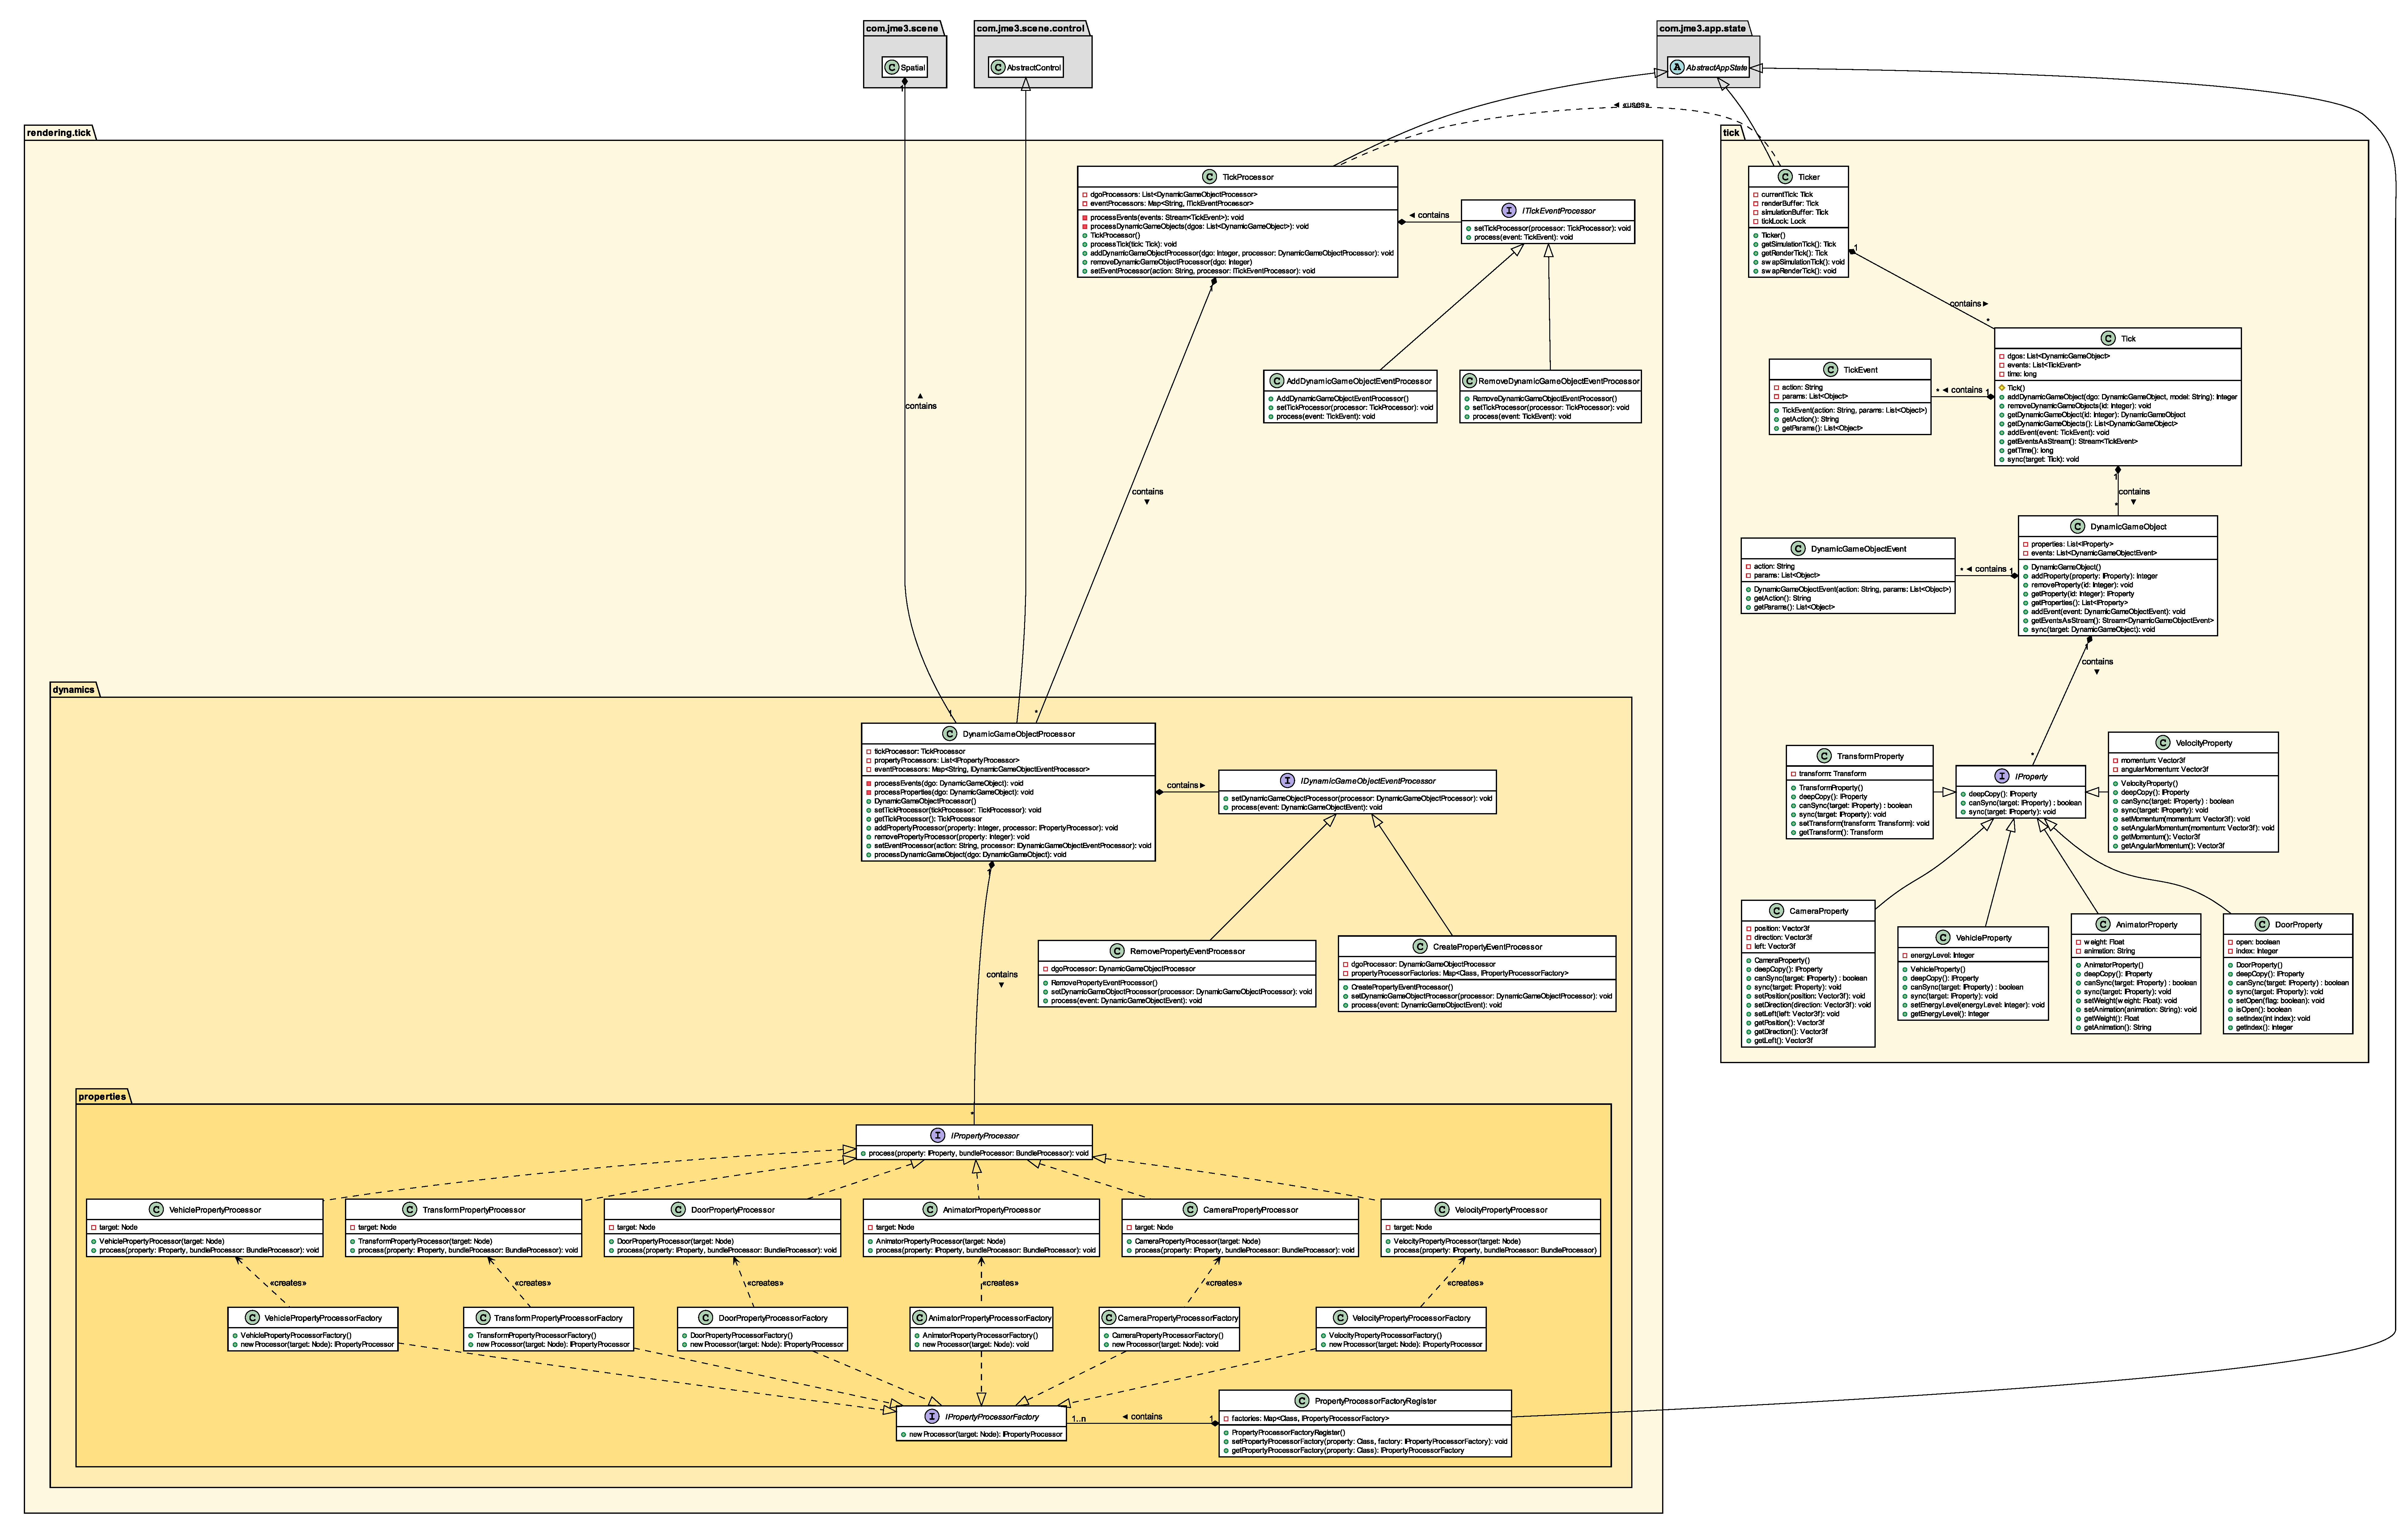
\includegraphics[width=\linewidth]{Interface/modul.eps}
    \caption{InGame - Interface Klassen-Diagram}
\end{figure}

\pagebreak
		\subsection{Assets}

Das Modul Assets bietet einfachen Zugriff auf als .j3o gespeicherte Modelle, indem pro Model ein Assetdeskriptor vorhanden ist, welcher
in Json geschrieben ist und von einem \textit{JsonModelProvider} gelesen und verarbeitet wird. Die Modelle liegen dann als Node vor und können so einfach
in den Scenegraph eingebunden werden. Ausserdem unterstützen \textit{AbstractModelProvider} (also auch \textit{JsonModelProvider}) das asynchrone Laden von Modellen
auf einem separaten Thread und das Updaten eines Ladebildschirms. Ein \textit{JsonModelProvider} lädt immer ein ebenfalls in Json beschriebenes \textit{AssetPack},
welches aus benannten Gruppierungen von Assets besteht.

\begin{figure}[htbp]
    \centering
    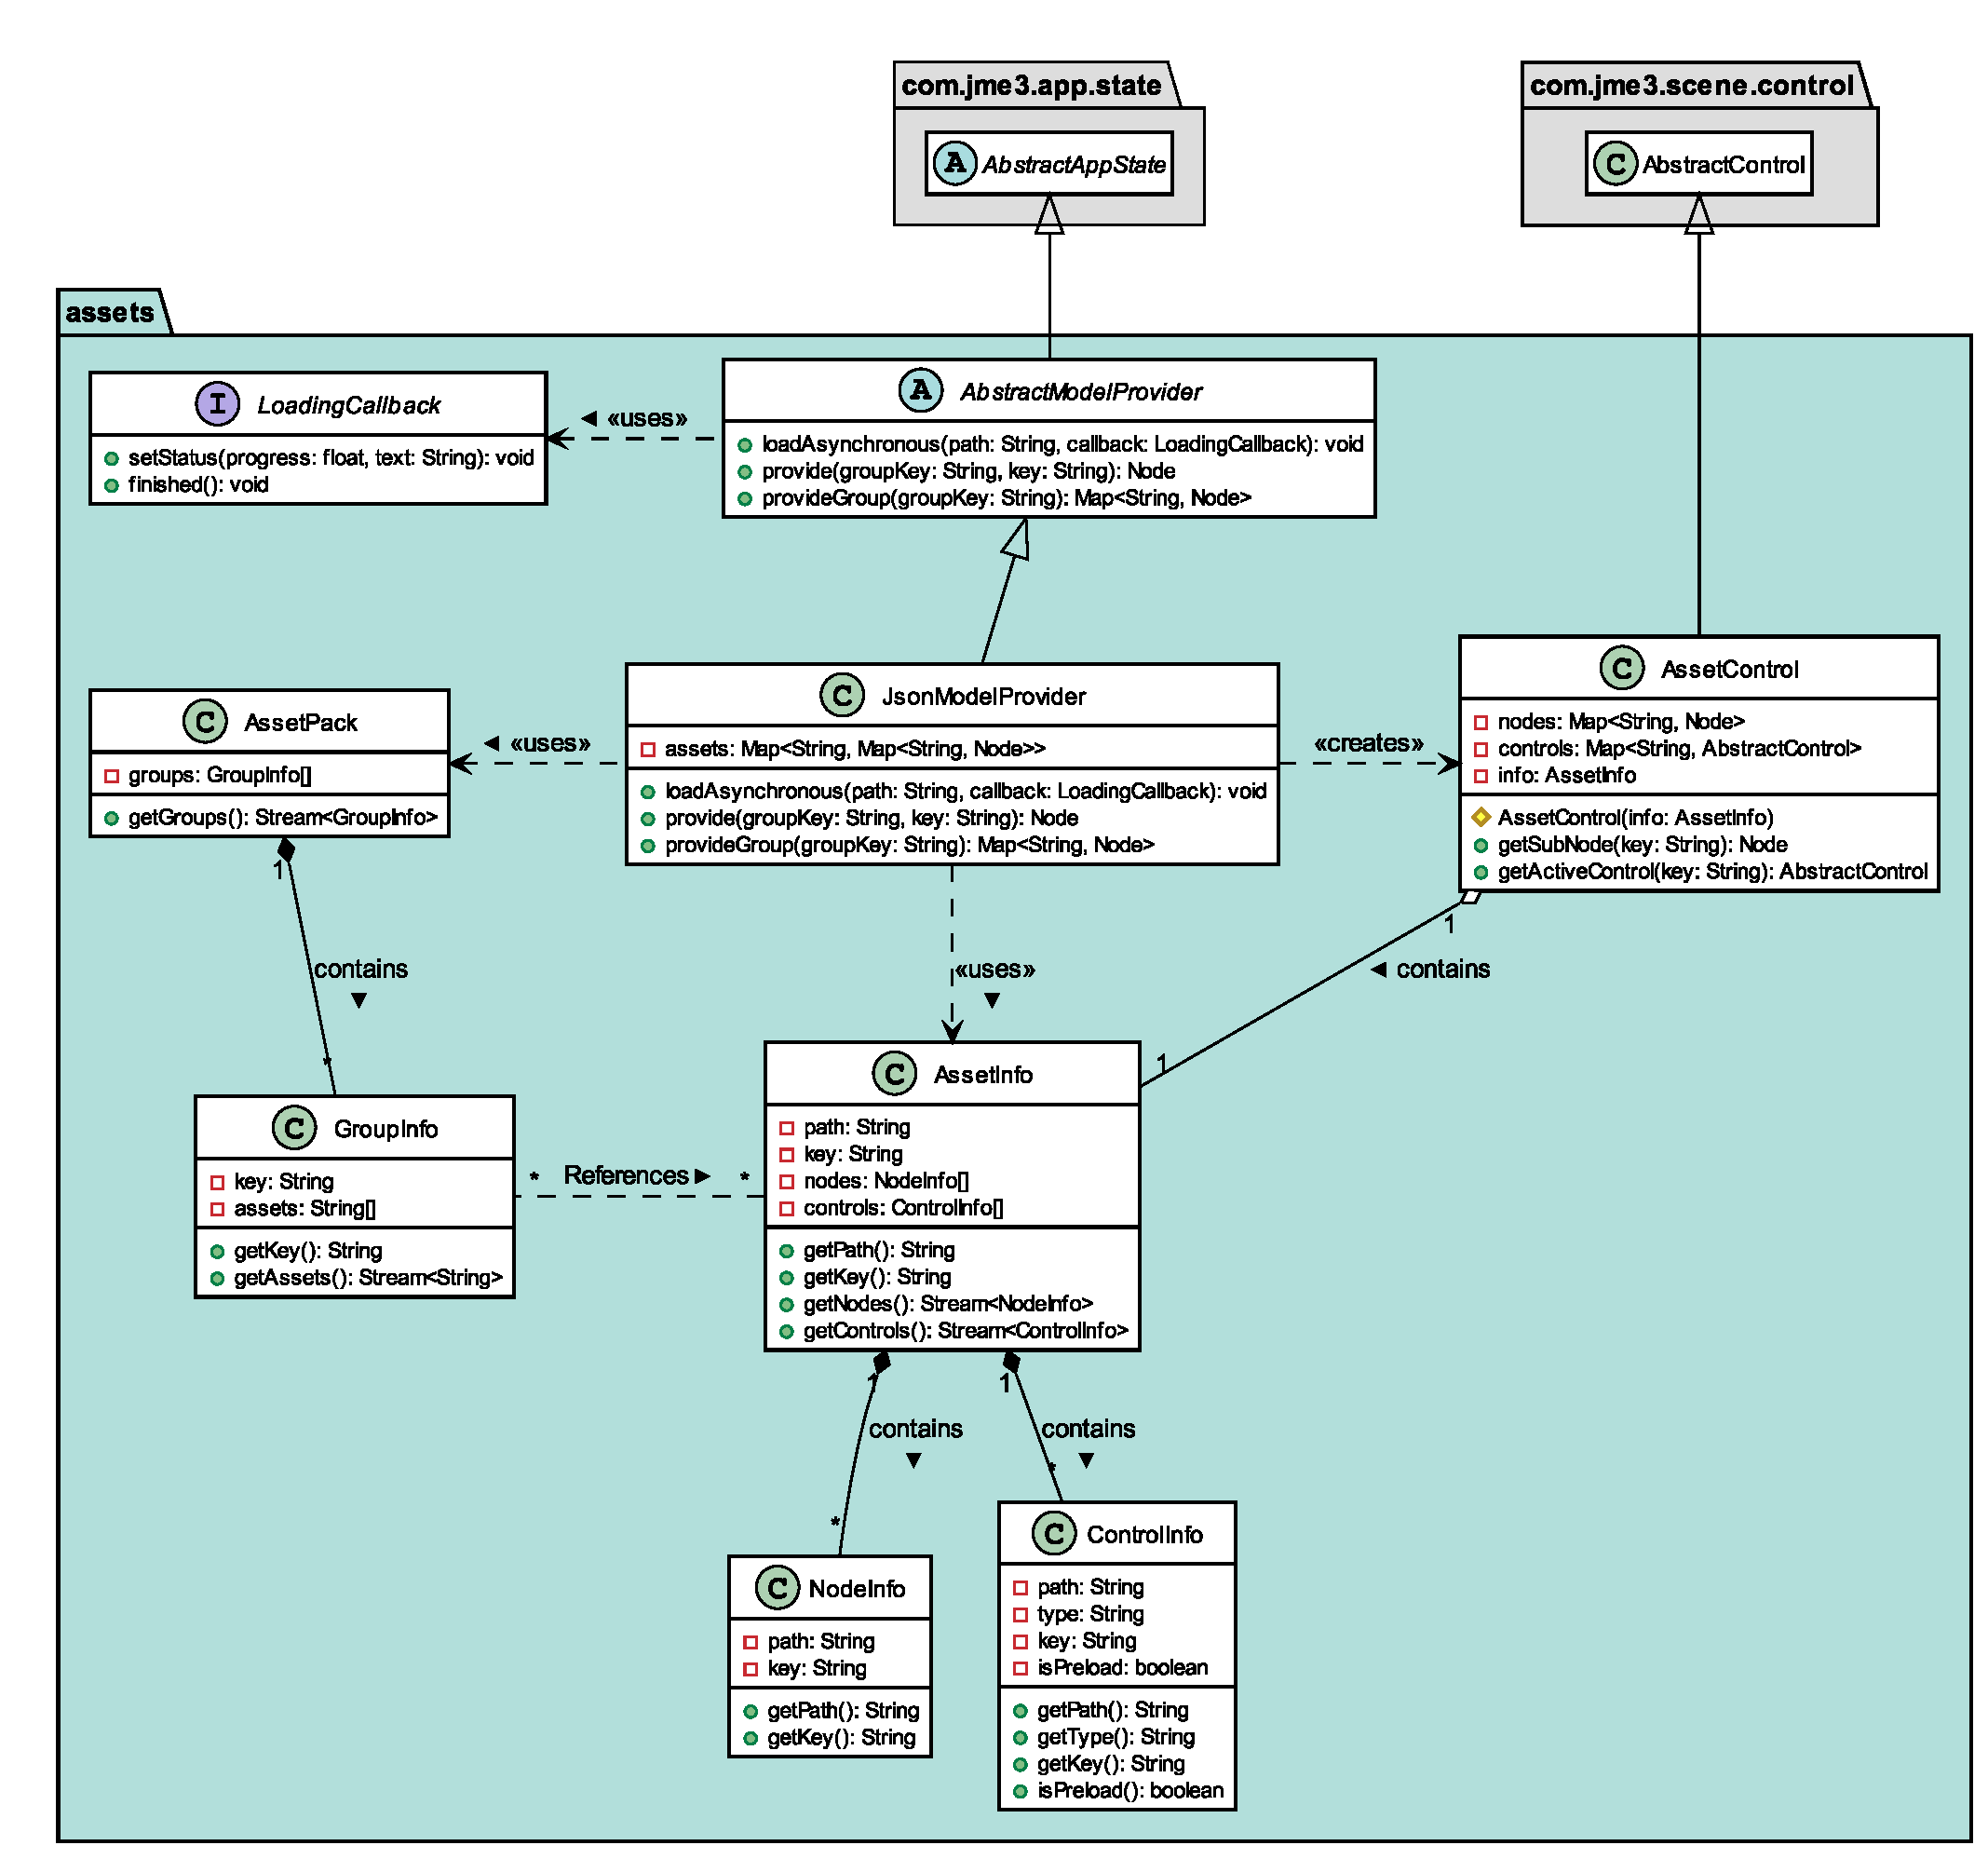
\includegraphics[width=\linewidth]{Assets/assets.eps}
    \caption{Assets Klassen-Diagram}
\end{figure}

\pagebreak

		\pagebreak
			
		\subsection{Generation}
			
			Das Modul \textit{Generation} wird verwendet um vor Spielbeginn eine Karte, abhängig von einem Seed, 
			zu generieren. Hierzu wird eine Schnittstelle \textit{IMapGenerator} angeboten, welche lediglich eine Methode zum 
			Generieren bereit stellt. Dieser gibt man einen Seed und eine RootNode für die Karte mit.\\
			Zum Generieren wird anhand einer Json - Datei ein Objekt der Klasse \textit{GenerationConfig} 
			erstellt, durch die der Generierungsprozess, anhand verschiedener Parameter, konfiguriert wird.\\

			Beginnt die eigentliche Generierung beim \textit{MapGenerator} so setzt dieser die Karte aus verschiedenen 
			Teilstücken zusammen. Um diese Teilstücke möglichst austauschbar zu halten, hat der \textit{MapGenerator} auf deren Generierungsprozess 
			keinen direkten Einfluss, sondern kann lediglich eine Hand voll 'Startparameter' für die Generierung festlegen. 
			Für jede Art von Teilstück hält der \textit{MapGenerator} genau einen entsprechenden Generator (z.B. \textit{IDomeGenerator}), 
			welcher sich um die Generierung aller Teilstücke des jeweiligen Types (z.B. \textit{IDome}) kümmert.\\

			Sind alle Teilstücke generiert und zu einer sinnvollen Strecke zusammengestzt worden, so ist der Generierungsprozess abgeschlossen, 
			und es wird ein \textit{IMapBody} erstellt, welcher alle notwendigen Bestandteile der Strecke für das andere Team beschreibt. 
			Außerdem wird der Scenegraph erstellt, um die Karte anzeigen zu können.\par
			
			\begin{figure}[htbp]
				\centering
				\includegraphics[scale=0.07,angle=0]{./Bilder/MapGenerator.pdf}
				\caption{Klassendiagramm Generationsmodul}
			\end{figure}
		
		\pagebreak
			
		\subsection{Menü}
			
			Im Modul Menü ist die grafische Benutzeroberfläche des Spiels realisiert. 
			Dabei hat jeder Menü-Bildschirm eine eigene Controller Klasse, welche das 
			Interface \textit{de.lessvoid.nifty.screen.ScreenController} implementiert, 
			um zwischen den Bildschirmen wechseln zu können, sowie Benutzeraktionen zu 
			steuern und umzusetzen. \\
			Ebenfalls implementiert jede Klasse das Interface 
			\textit{de.lessvoid.nifty.screen.KeyInputHandler}, um auf Benutzereingaben 
			reagieren zu können. Dabei wird die Klasse~\nameref{mim} benutzt, welche 
			Eingaben auf ein NiftyInputEvent konvertiert. Dadurch, dass die Klassen auf
			NiftyInputEvents reagieren, kann das Mapping individuell angepasst werden. 
			Unter anderem können so leicht GamePads oder Ähnliches integriert werden, 
			da nicht alle Methoden überarbeitet werden müssen, sondern lediglich ein 
			Mapping implementiert werden muss. \\
			Außerdem erben einige Methoden von der Klasse 
			\textit{com.jme3.app.state.AbstractAppState} um Zugriff auf die Applikation 
			zu haben. Dadurch kann aus dem Menü zum Beispiel das Spiel beendet werden. \\
			Das Menü Modul dient auch als Schnittstelle zur Grafik- und Streckengenerierung,
			sowie zum anderen Team des PSE-Projektes. \par

			\begin{center}
				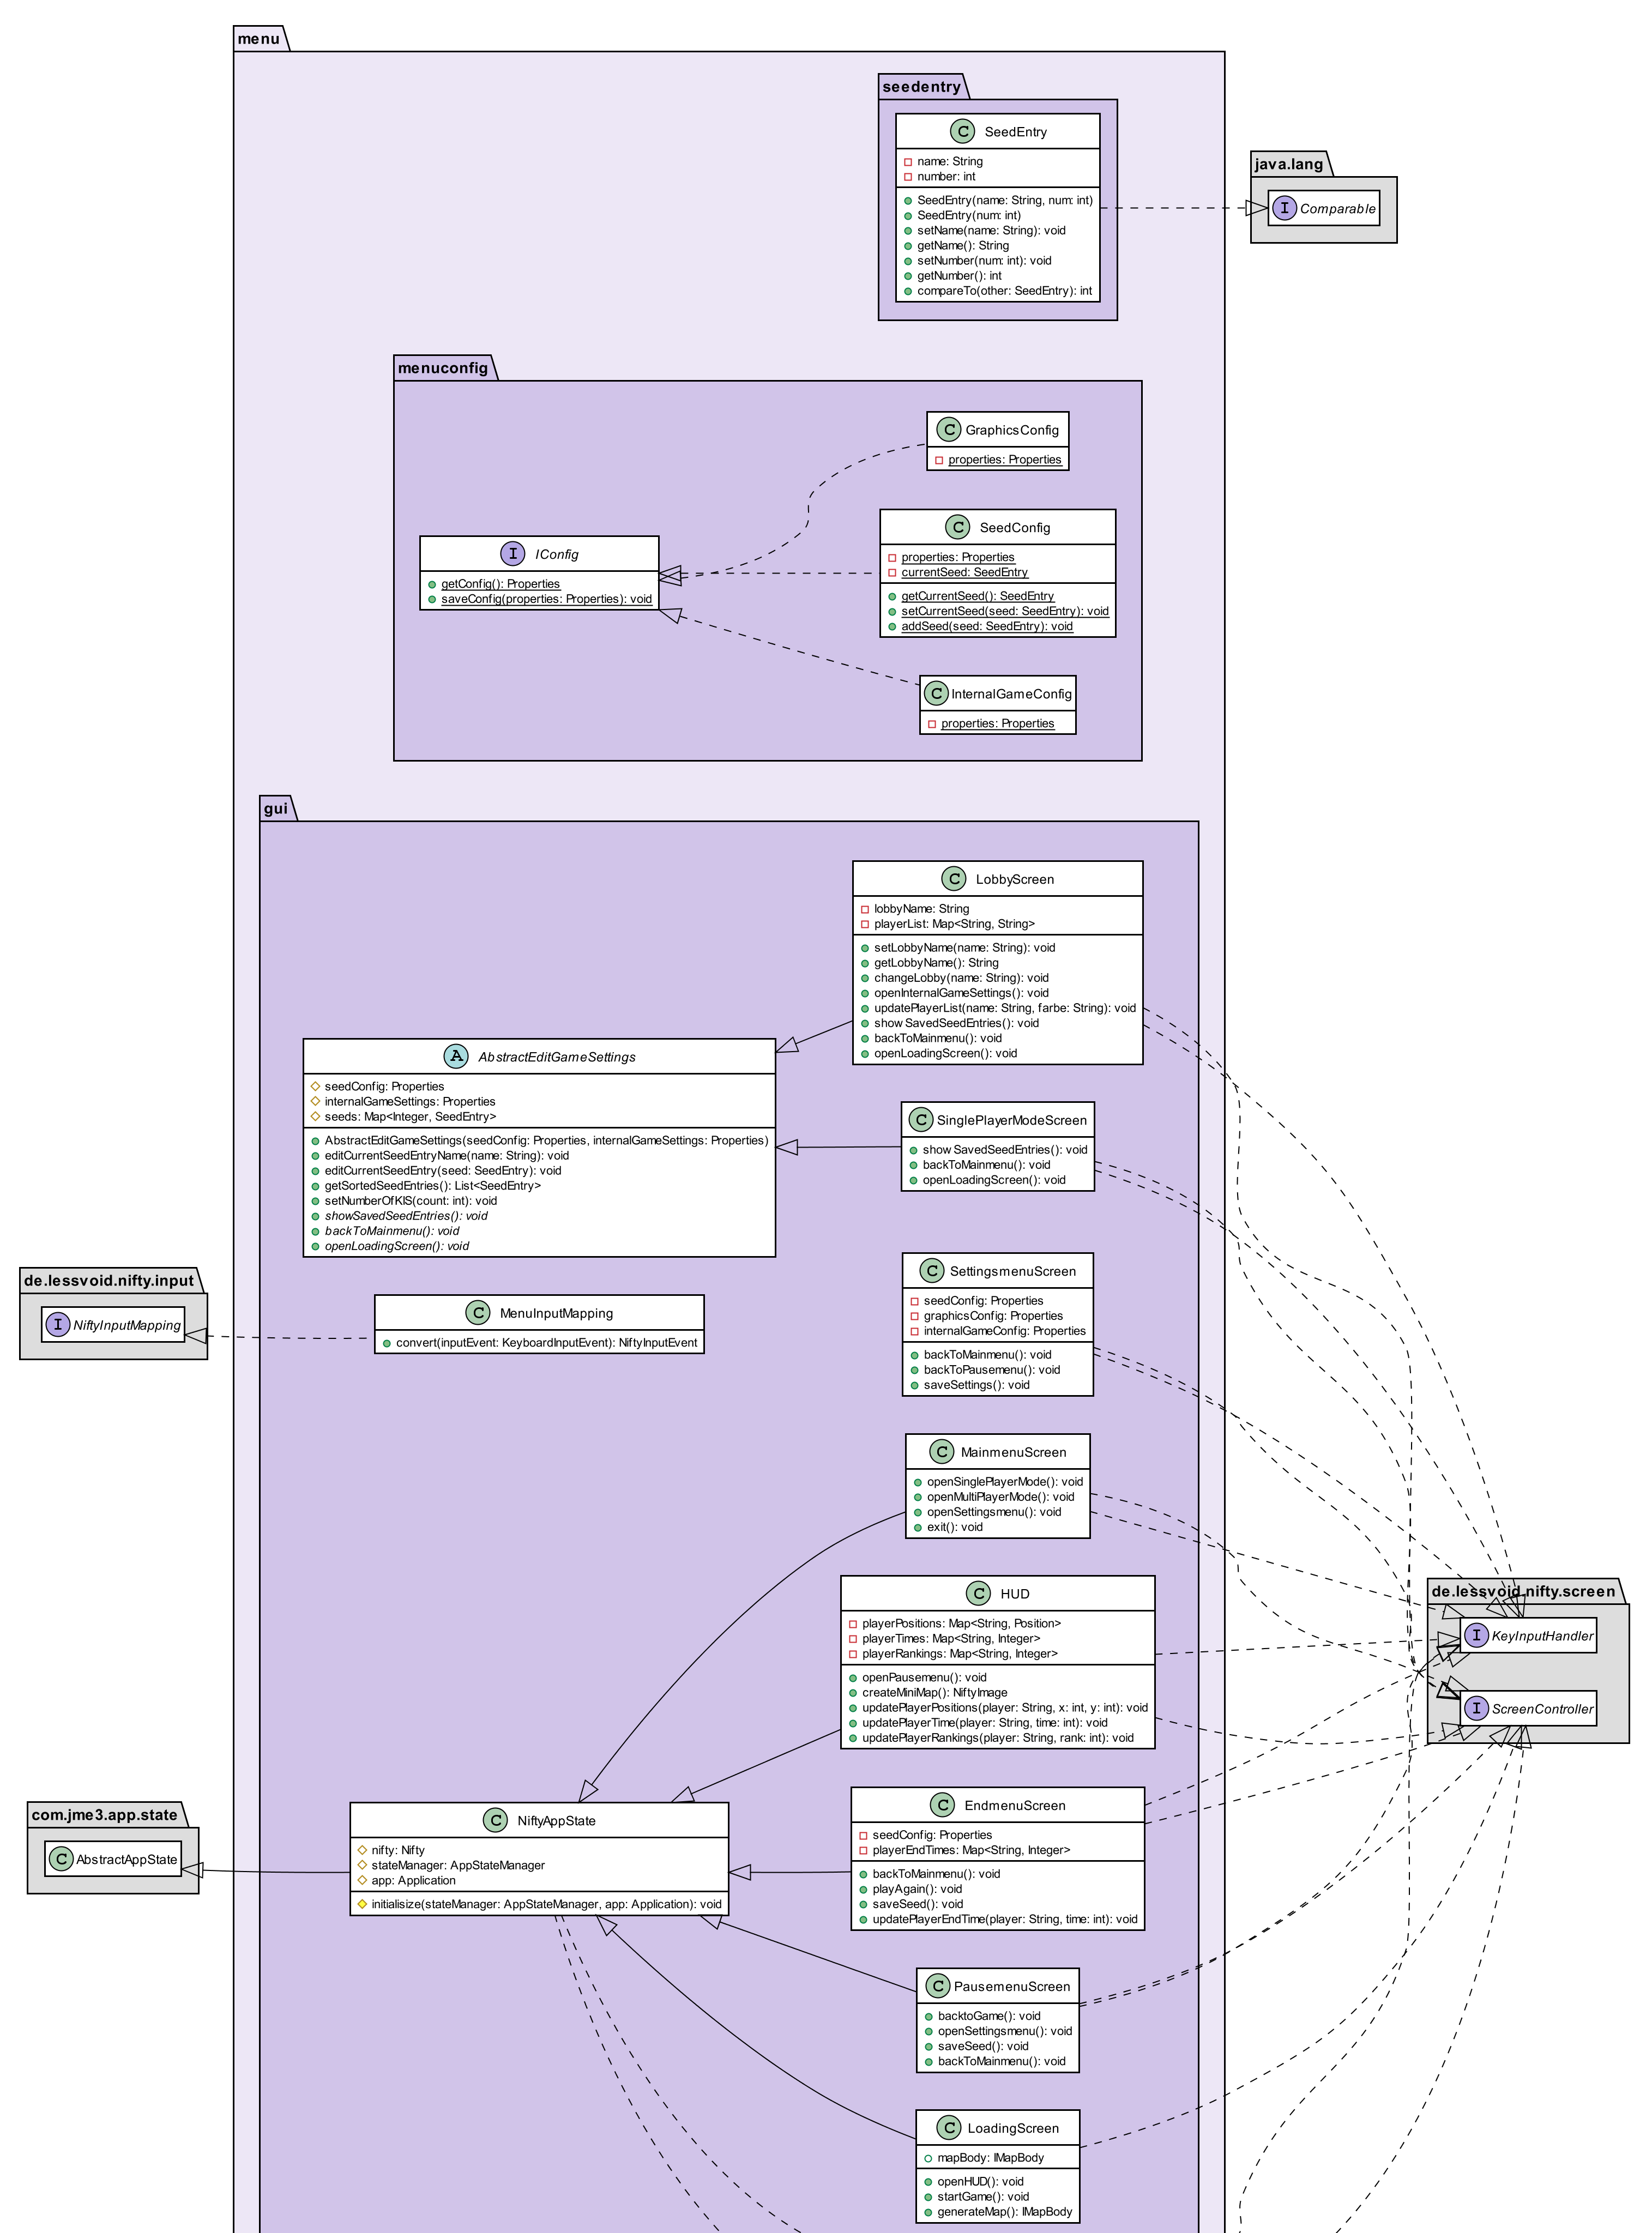
\includegraphics[width=0.9\linewidth]{./GUI/GUI_Bilder/GUIAll.pdf}
				\captionof{figure}{Klassendiagramm Menü}
				\label{fig:menu}
			\end{center}

	\pagebreak
	
	\section{Klassenübersicht}
	
		\subsection{InGame - Grafik}

            \subsubsection{effects}
        Enthält die verwendeten Effekte die später zu unserer Szene hinzugefügt
        werden. Eine essenzielle Bedeutung kommt dabei den verschiedenen Partikeleffekten
        zu. \par
        \begin{figure}[htbp]
            \centering
            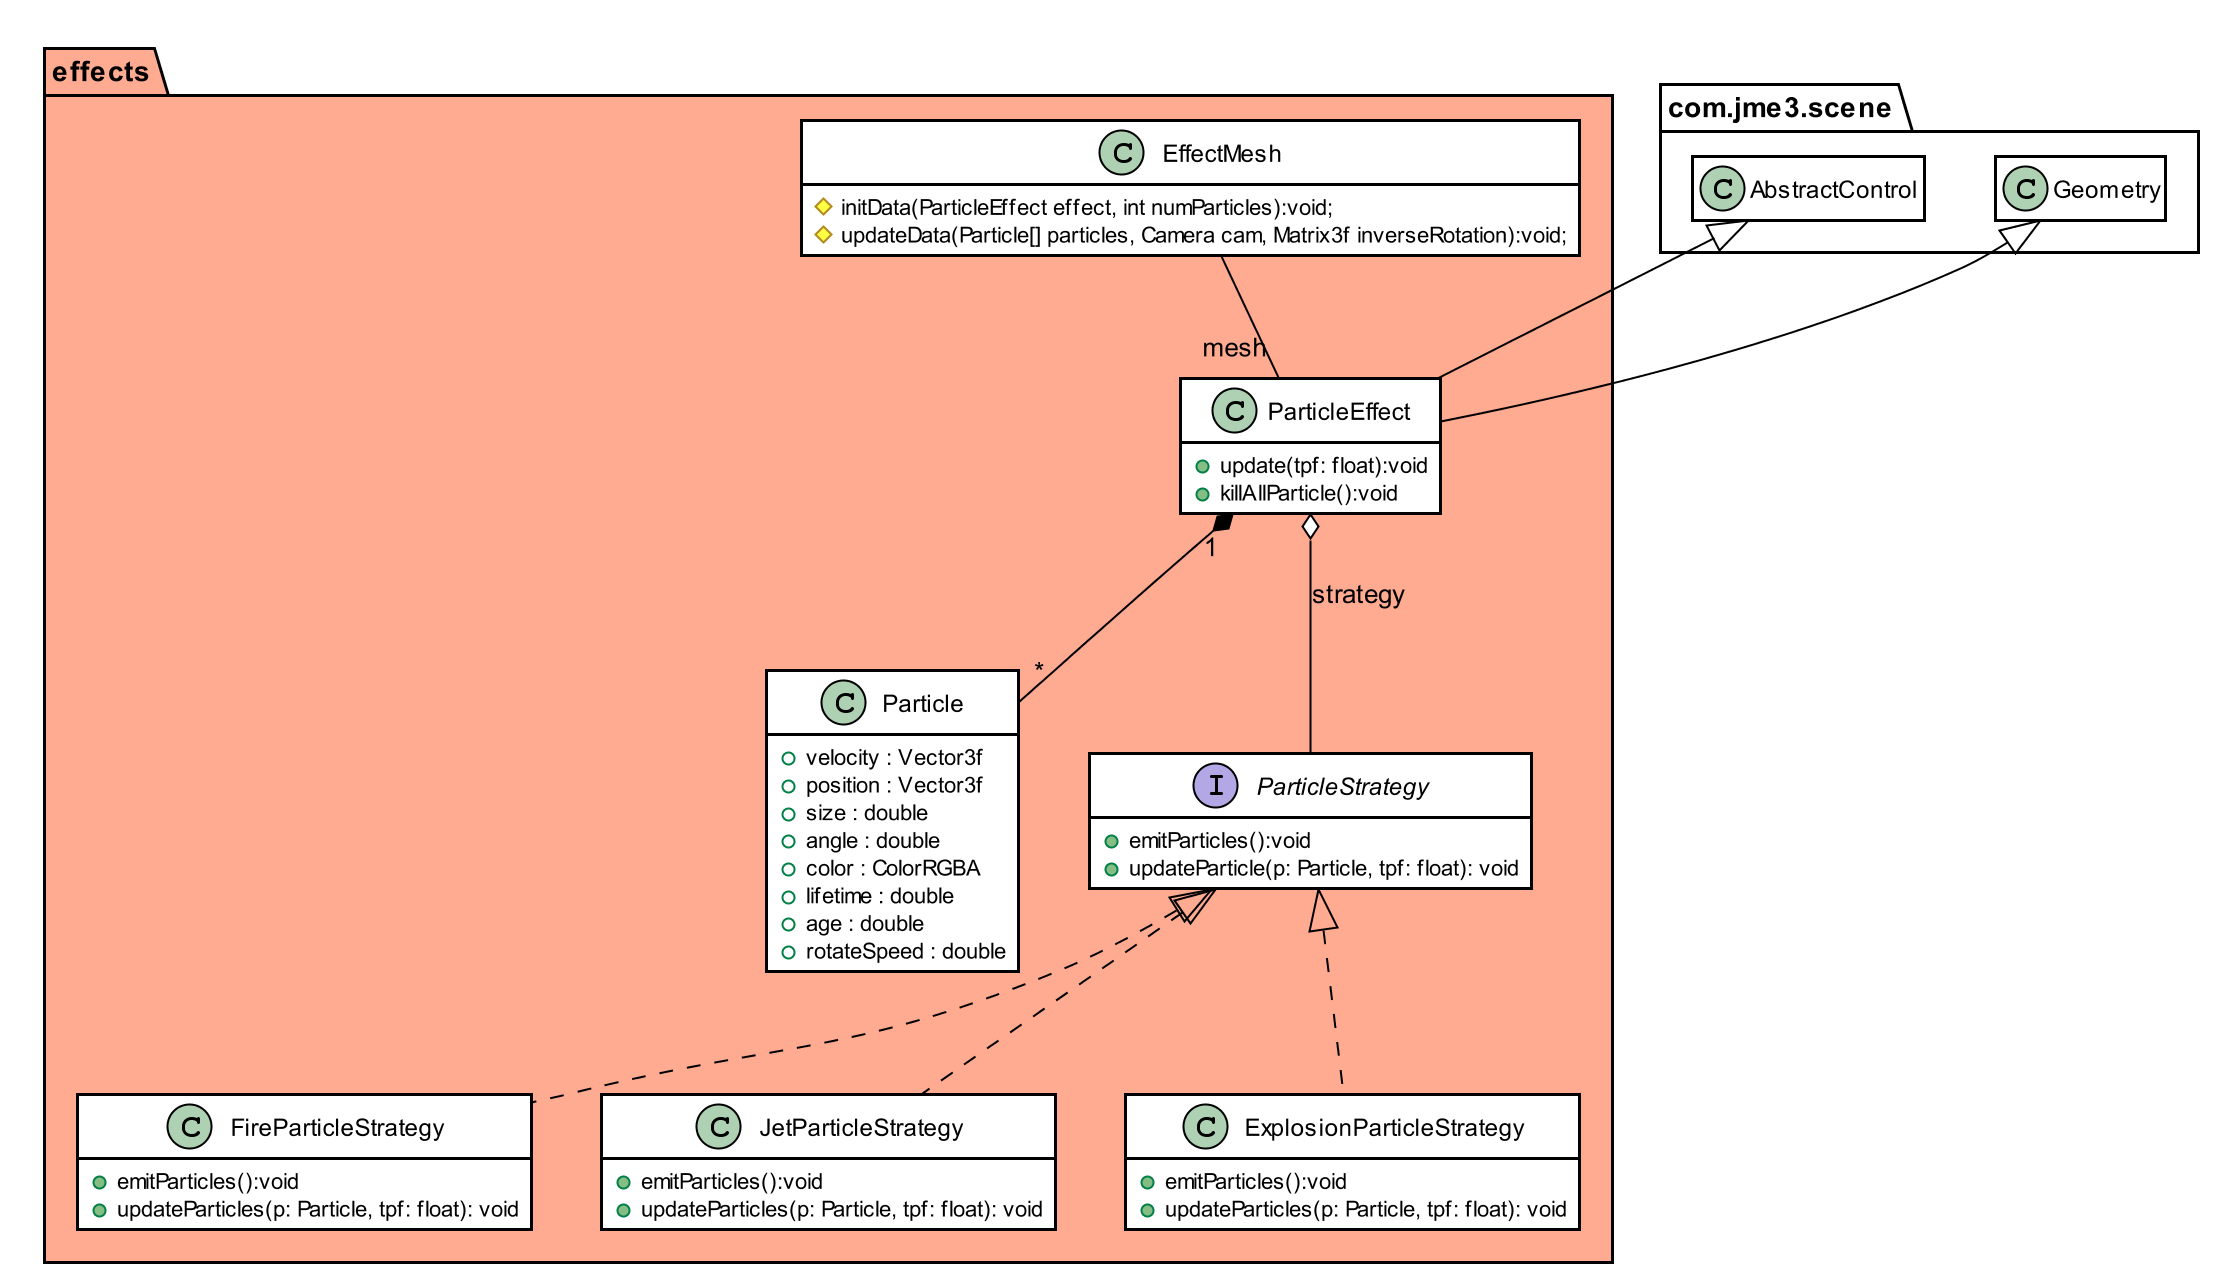
\includegraphics[width=1\linewidth]{InGameGrafik/Bilder/particleeffect.png}
            \caption{Klassendiagramm effects}
        \end{figure}
            \paragraph{\underline{Particle}} \mbox{}\\
                Repräsentiert die abstrakte Beschreibung eines einzelnen Partikels.
                Alle zur weiteren Berechnung wichtigen Informationen des Partikels für den 
                Partikeleffekt sind hierin festgehalten. \par
                \textbf{Attribute}
                \begin{itemize}
                    \item \textit{velocity}
                        \begin{leftbar}[0.9\linewidth]
                        Richtungsvektor unserer Partikels in der dreidimensionalen Szene.   
                        \end{leftbar}
                    \item \textit{position}
                        \begin{leftbar}[0.9\linewidth]
                        Positionsvektor unseres Partikels in der Szene; Angegeben für den Objektsraum.
                        \end{leftbar}
                    \pagebreak
                    \item \textit{size}
                        \begin{leftbar}[0.9\linewidth]
                        Beschreibt aktuelle Größe des Partikels.   
                        \end{leftbar}
                    \item \textit{angle}
                        \begin{leftbar}[0.9\linewidth]
                        Ausrichtung des Partikels in der Szene.   
                        \end{leftbar}    
                    \item \textit{color}
                        \begin{leftbar}[0.9\linewidth]
                        Aktuelle Farbe des Partikels in der Szene.  
                        \end{leftbar}
                    \item \textit{lifetime}
                        \begin{leftbar}[0.9\linewidth]
                        Beschreibt die Lebenszeit des Partikels in der Szene. Also wie lange sich
                        er bewegt bevor er an Ausgangspunkt gesetzt wird.   
                        \end{leftbar}
                    \item \textit{age}
                        \begin{leftbar}[0.9\linewidth]
                        Aktuelles Alter des Partikels, also vergangene Schritte seit emittieren.   
                        \end{leftbar}
                    \item \textit{rotateSpeed}
                        \begin{leftbar}[0.9\linewidth]
                        Beschreibt wie schnell sich der Partikel um seine eigene Achse dreht.  
                        \end{leftbar}
                \end{itemize}

                \paragraph{\underline{ParticleEffect}}\mbox{}\\
                    Eine Art Geometry im Kontext der JMonkeyEngine. So kann der Effect später einfach
                    zu seinem korrespndierenden Objekt in den Scenegraph hinzugefügt werden.
                    Zu einem ParticleEffect gehört immer eine entsprechende Anzahl von Partikeln.
                    \par

                    \textbf{Methoden}
                    \begin{itemize}
                        \item \textit{update(float tpf): void}
                            \begin{leftbar}[0.9\linewidth]
                            Aktualisiert den Partikeleffekt anhand der Strategy, sowie der framerate.  \\ 
                            \textbf{@param tpf} Times per frame.\\
                            \end{leftbar}
                        \item \textit{killAllParticle():void}
                            \begin{leftbar}[0.9\linewidth]
                            Lässt den Partikeleffekt wieder verschwinden.  
                            \end{leftbar}
                    \end{itemize}

                \pagebreak
                \paragraph{\underline{JetParticleStrategy}}\mbox{}\\
                    Beschreibt die genaue Strategie anhand der Partikel an einer Düse
                    emittiert werden.\par

                    \textbf{Methoden}
                    \begin{itemize}
                        \item \textit{emitParticles():void}
                            \begin{leftbar}[0.9\linewidth]
                            Emittiert einen einzigen Partikel nach "unten" in einem schmalen 
                            zufälligen Kegelradius .  
                            \end{leftbar}
                        \item \textit{updateParticles(Particle p, float tpf): void}
                            \begin{leftbar}[0.9\linewidth]
                            Aktualisiert die Partikel damit sie wie Düsenpartikel aussehen.\\  
                            \textbf{@param p} Der aktuelle Partikel der aktualisiert werden soll.\\
                            \textbf{@param tpf} Dime per frame.\\
                            \end{leftbar}
                    \end{itemize}
                
                \paragraph{\underline{FireParticleStrategy}}\mbox{}\\
                    Beschreibt die Strategie für Partikel von Feuer. Sie sollen ihre Farbe ändern
                    und sich von einem zentralen Punkt von Innen nach Außen bewegen.\par

                    \textbf{Methoden}
                    \begin{itemize}
                        \item \textit{emitParticles():void}
                            \begin{leftbar}[0.9\linewidth]
                            Wie ein einzelnes Feuerpartikel emittiert werden soll; zuälliger Winkel über
                            360 Grad mit sich ändernder Größe.   
                            \end{leftbar}
                        \item \textit{updateParticles(Particle p, float tpf): void}
                            \begin{leftbar}[0.9\linewidth]
                            Verändert die Attribute eines Feuerpartikels regelmäßig(abhängig von framerate).\\
                            \textbf{@param p} Der aktuelle Partikel der aktualisiert werden soll.\\
                            \textbf{@param tpf} Time per frame.\\
                            \end{leftbar}
                    \end{itemize}

                \pagebreak
                \paragraph{\underline{ExplosionParticleStrategy}}\mbox{}\\
                    Ist die Strategie wie ein PartikelEffekt für eine Explosion gesteuert
                    werden soll. \par

                    \textbf{Methoden}
                    \begin{itemize}
                        \item \textit{emitParticles():void}
                            \begin{leftbar}[0.9\linewidth]
                            Ein einzelner Explosionspartikel soll auf bestimmter Art und Weise emittiert werden
                            von einem Punkt aus in alle Richtungen.\\   
                            \end{leftbar}
                        \item \textit{updateParticles(Particle p, float tpf): void}
                            \begin{leftbar}[0.9\linewidth]
                            Aktualisiert die Attribute eines einzigen Partikels um eine Explosion zu sehen.
                            So wird die Geschwindigkeit, Position, Farbe etc. verändert.\\    
                            \textbf{@param p} Der aktuelle Partikel der aktualisiert werden soll.\\
                            \textbf{@param tpf} Time per frame.\\
                            \end{leftbar}
                    \end{itemize}
        \pagebreak
    \subsubsection{postprocessing}
        Grundlegende Struktur des Postprocessing; beschreibt die Einbindung des 
        MotionBlurFilter in die JMonkeyEngine vorgaben\par
        \begin{figure}[htbp]
            \centering
            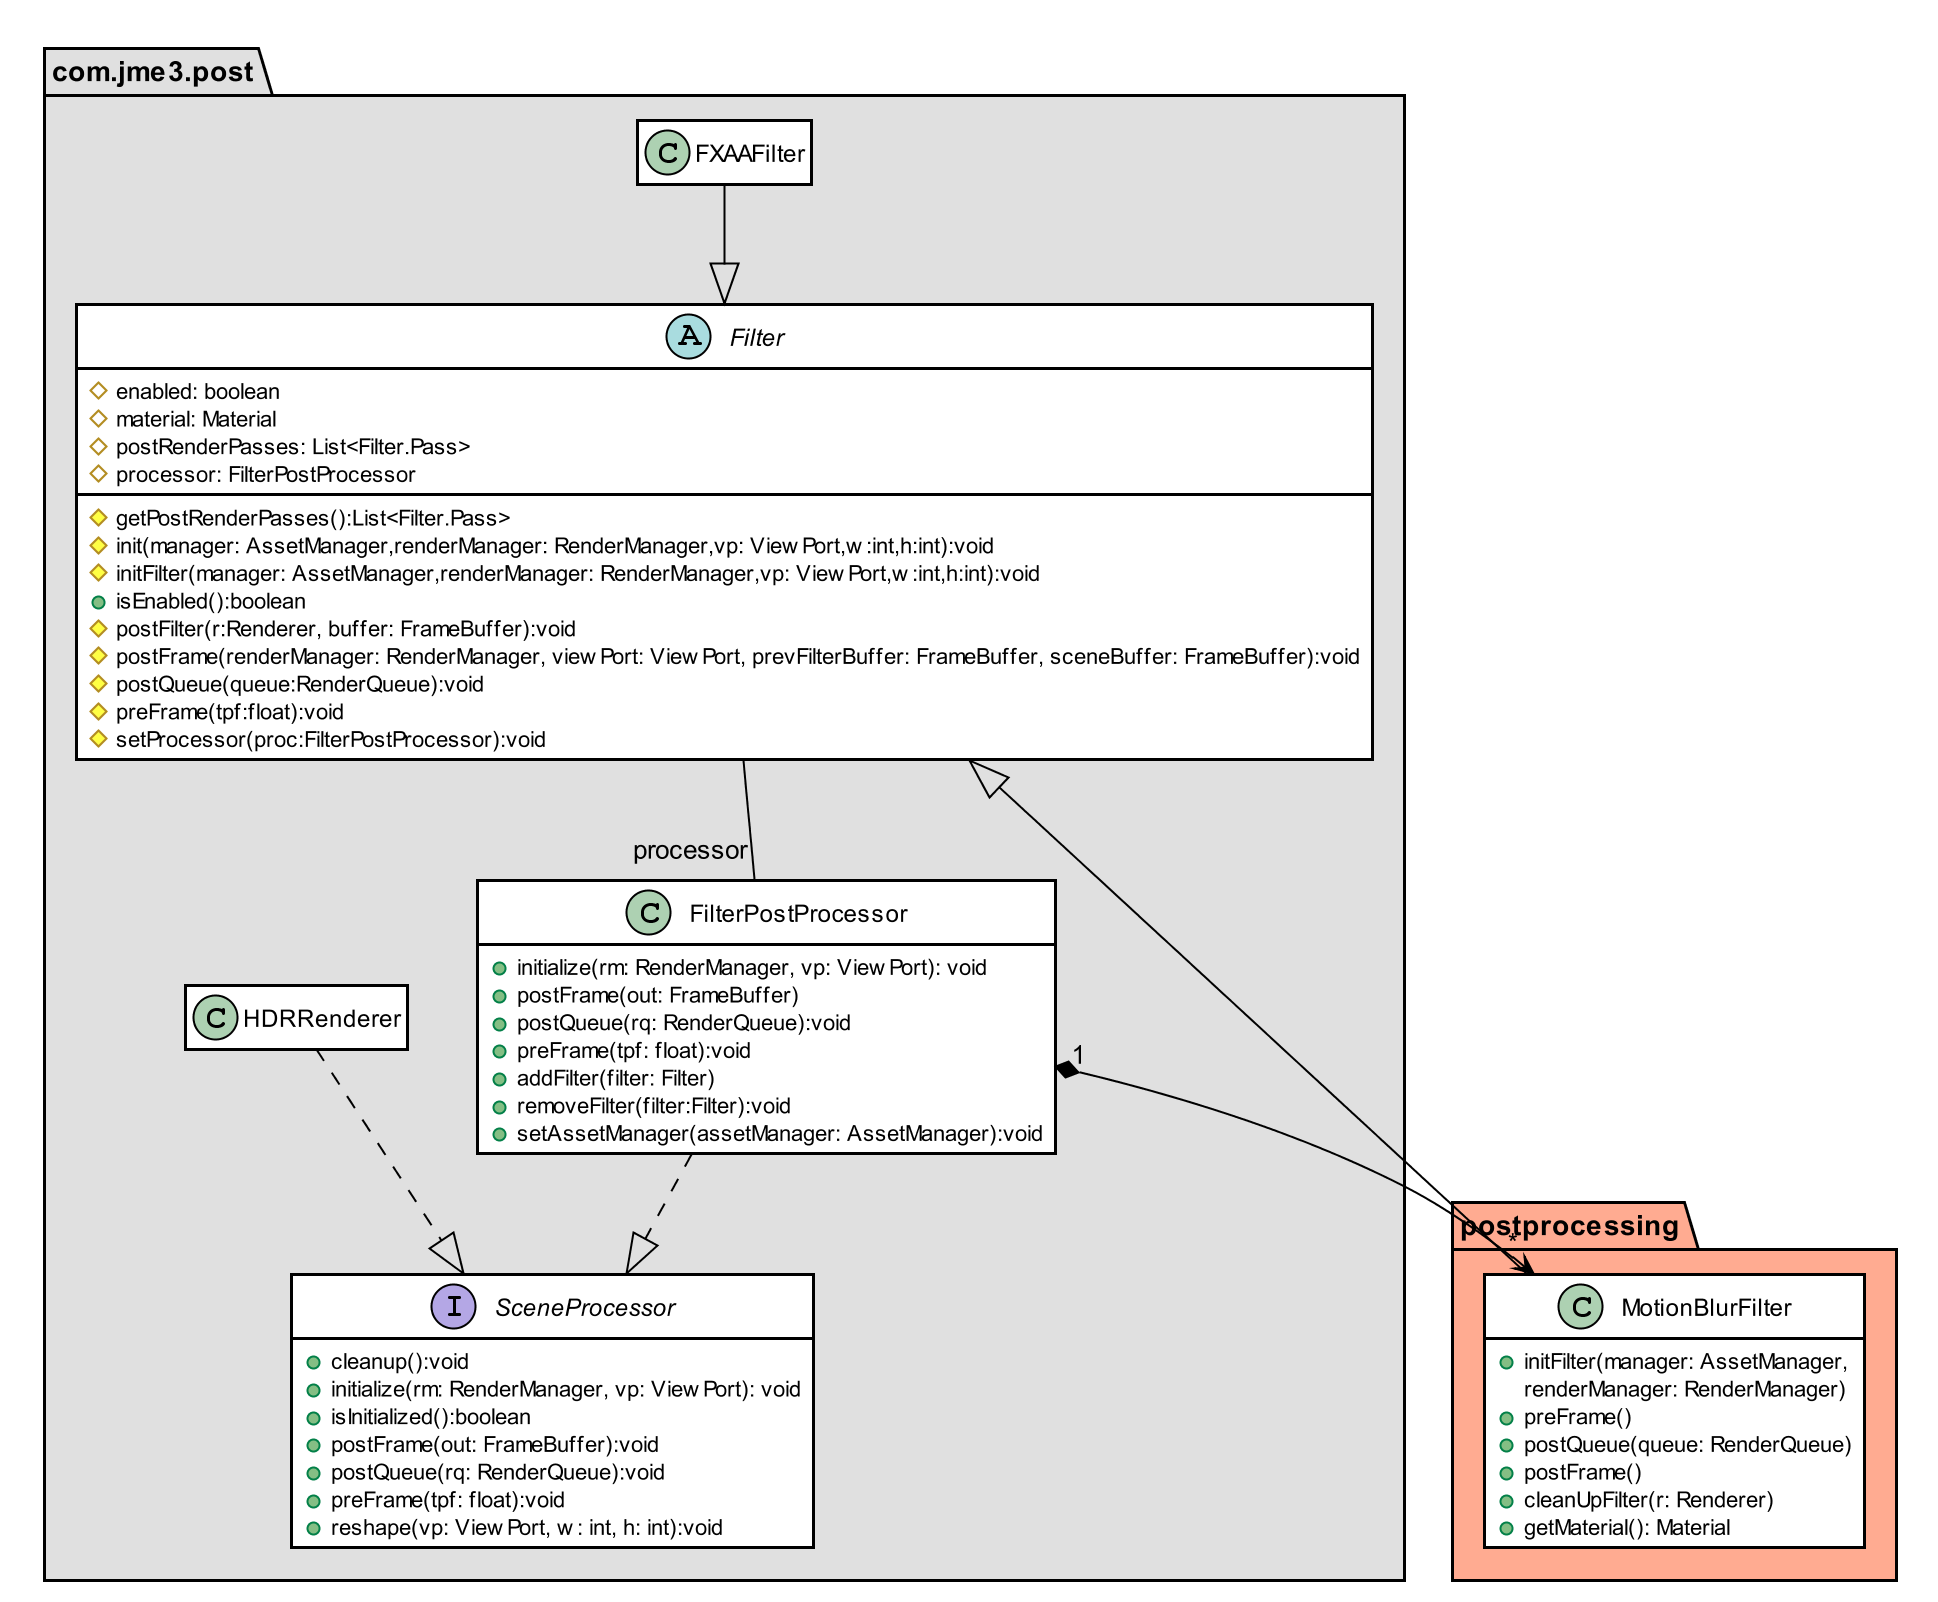
\includegraphics[width=1\linewidth]{InGameGrafik/Bilder/postprocessing.png}
            \caption{Klassendiagramm postprocessing}
        \end{figure}
            \paragraph{\underline{MotionBlurFilter}} \mbox{}\\
                    Visueller Effekt der Bewegungsunschärfe.\par
\pagebreak   
    \subsubsection{animation}
    Benötigte Klassen sowie ihre Schnittstellen zu dem Interface, dass bereits von der 
    JMonkeyEngine vorgegeben wird um (eine/mehrere) Animationen zu realisieren. \par
    \begin{figure}[htbp]
        \centering
        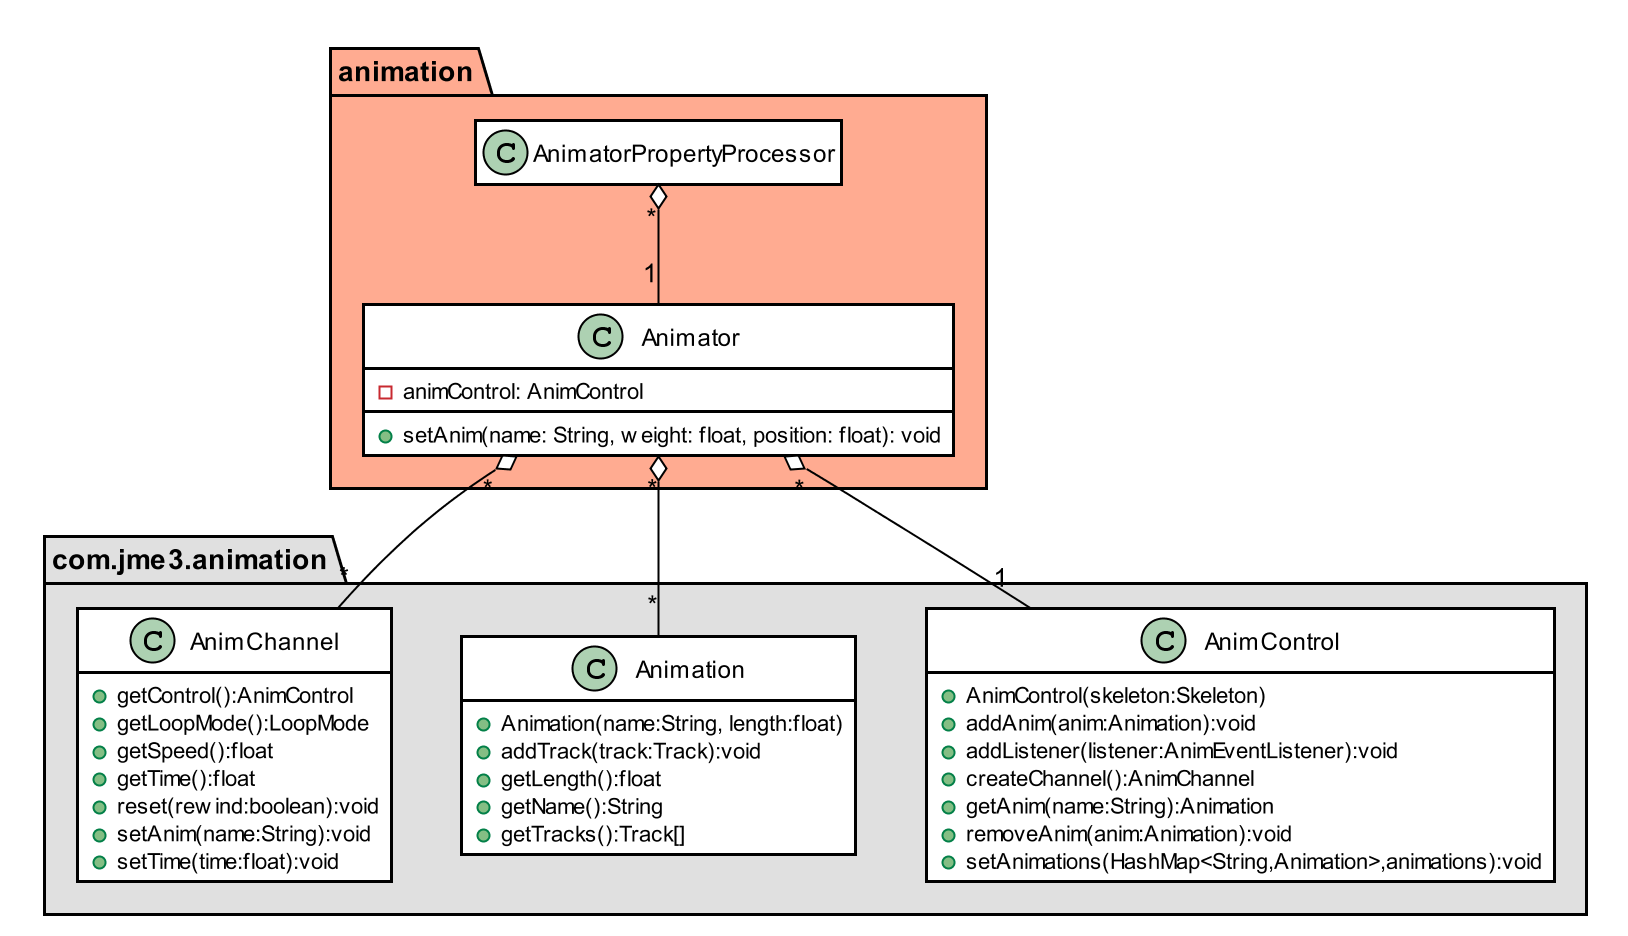
\includegraphics[width=1\linewidth]{InGameGrafik/Bilder/animation.png}
        \caption{Klassendiagramm animation}
    \end{figure}
    \paragraph{\underline{Animator}} \mbox{}\par
                Klasse zur Steuerung einer Animation.\par
                
                \textbf{Attribute}
                \begin{itemize}
                    \item  \textit{animControl} 
                        \begin{leftbar}[0.9\linewidth]
                        Kontroller zur Steuerung der Animation.  
                        \end{leftbar}
                \end{itemize}

                \textbf{Methoden}					
                \begin{itemize}
                    \item  \textit{setAnim(String name, float weight, float position): void}
                        \begin{leftbar}[0.9\linewidth]
                            Setzt eine Animation auf der Scene.\\
                            \textbf{@param name} Name der Animation.\\
                            \textbf{@param weight} "Gewicht der Animation".\\
                            \textbf{@param position} Position der Animation innerhalb der Scene.
                        \end{leftbar}   
                \end{itemize}
\pagebreak
    
    \pagebreak
		\subsection{InGame - Interface}

\subsubsection{tick}
    Enthält die Datenstruktur Tick und Funktionalität um die Datenstruktur zwischen Simulations- und RenderThread zu übergeben.

    \begin{figure}[htbp]
        \centering
        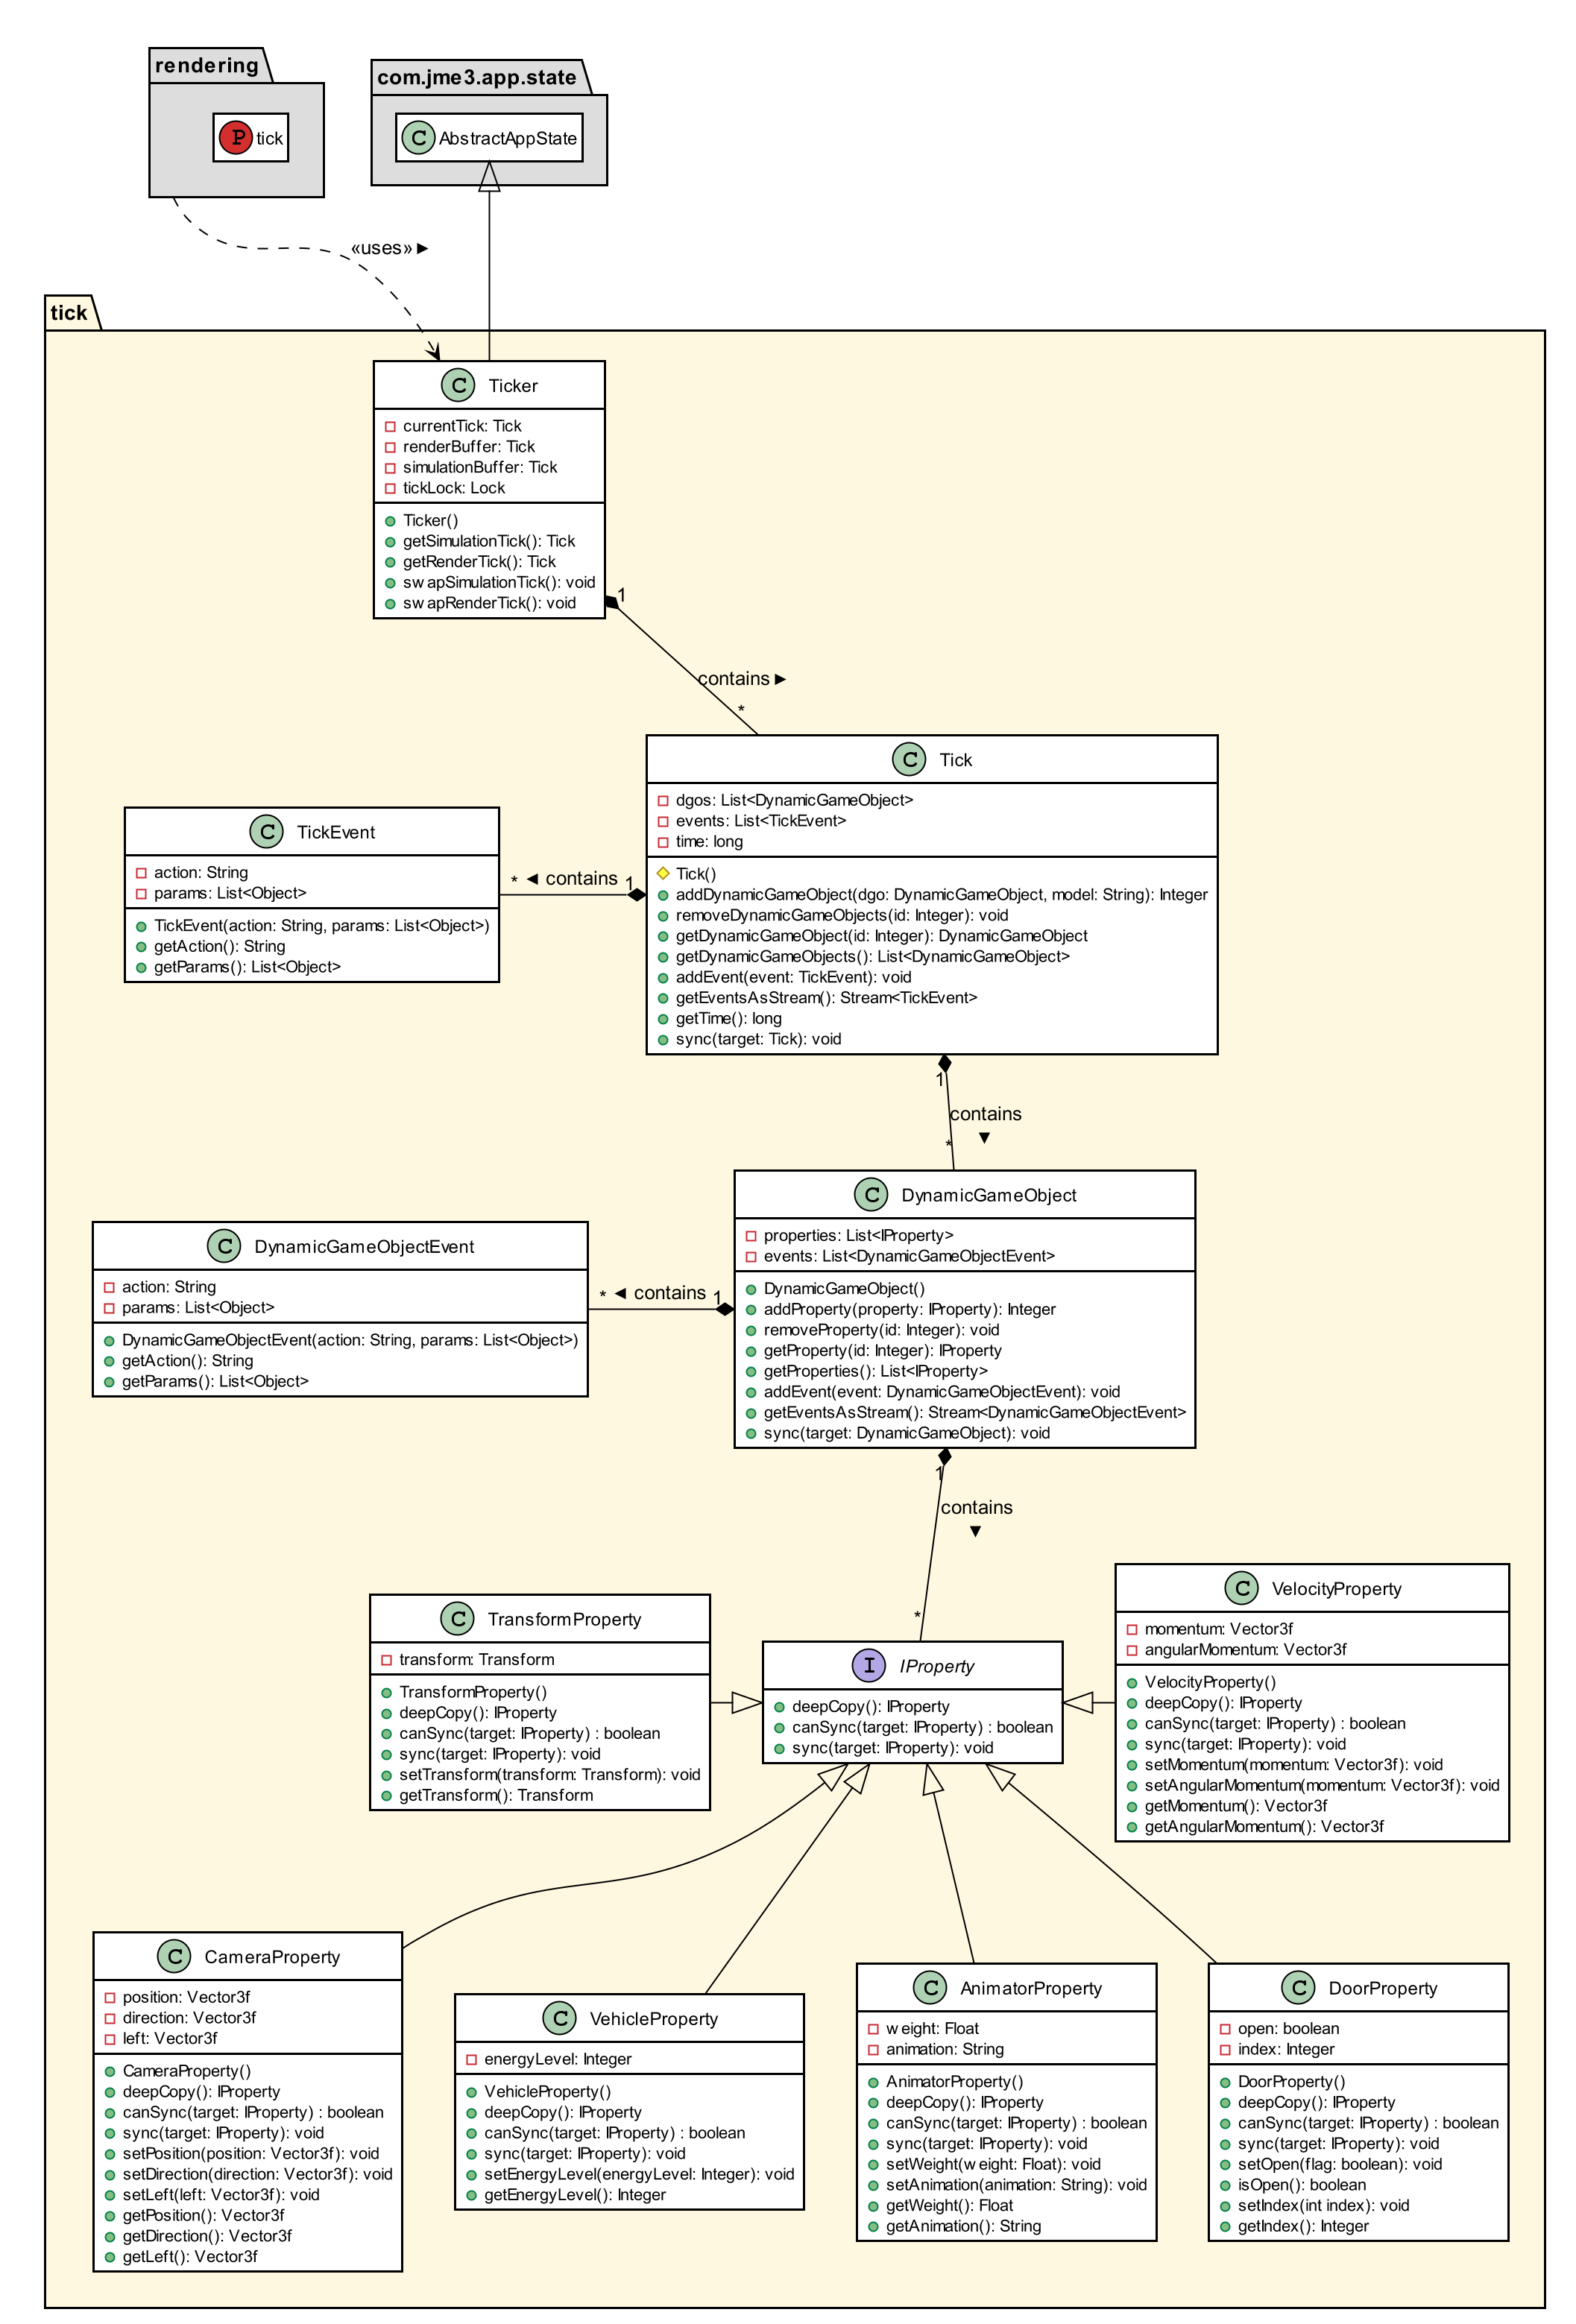
\includegraphics[width=0.72\linewidth]{Interface/tick.png}
        \caption{tick Klassen-Diagram}
    \end{figure}

    \paragraph{\underline{Ticker}} \mbox{}\\
    \\
        AbstractAppState, welcher die Buffer für triple-buffering zwischen Simulations- und RenderThread hält und das triple-buffering kontrolliert.\par
        
        \textbf{Attribute}
        \begin{itemize}
            \item \textit{- Tick simulationBuffer}
                \begin{leftbar}[0.9\linewidth]
                    \textit{Tick} welcher vom SimulationsThread verwendet wird.
                \end{leftbar}
            \item \textit{- Tick renderBuffer}
                \begin{leftbar}[0.9\linewidth]
                    \textit{Tick} welcher vom RenderThread verwendet wird.
                \end{leftbar}
            \item \textit{- Tick currentTick}
                \begin{leftbar}[0.9\linewidth]
                    \textit{Tick} welcher den aktuellsten stand der Szene hält.
                \end{leftbar}
            \item \textit{- Lock tickLock}
                \begin{leftbar}[0.9\linewidth]
                    Wird verwendet um die Zugriffe auf die Methoden \textit{Ticker.swapSimulationBuffer} und \textit{Ticker.swapRenderBuffer}
                    zu synchronisieren.
                \end{leftbar}
        \end{itemize}

        \textbf{Methoden}
        \begin{itemize}
            \item \textit{+ Ticker()}
                \begin{leftbar}[0.9\linewidth]
                    Erstellt einen neuen \textit{Ticker} und initialisiert simulationBuffer, renderBuffer und currentTick als neuen \textit{Tick} und tickLock
                    als neues ReentrantLock.
                \end{leftbar}
            \item \textit{+ getSimulatioTick(): Tick}
                \begin{leftbar}[0.9\linewidth]
                    \textbf{@return} den \textit{Tick}, welcher vom SimulationsThread verwendet wird.
                \end{leftbar}
            \item \textit{+ getRenderTick(): Tick}
                \begin{leftbar}[0.9\linewidth]
                    \textbf{@return} den \textit{Tick}, welcher vom RenderThread verwendet wird.
                \end{leftbar}
            \item \textit{+ swapSimulationTick(): void}
                \begin{leftbar}[0.9\linewidth]
                    Überträgt den stand von simulationBuffer in currentTick.
                \end{leftbar}
            \item \textit{+ swapRenderTick(): void}
                \begin{leftbar}[0.9\linewidth]
                    Überträgt den stand von currentTick in renderBuffer.
                \end{leftbar}
        \end{itemize}

    \pagebreak
    \paragraph{\underline{Tick}} \mbox{}\\
    \\
        Enthält alle \textit{DynamicGameObject}s und \textit{TickEvent}s.\par
        
        \textbf{Attribute}
        \begin{itemize}
            \item \textit{- List<DynamicGameObject> dgos}
                \begin{leftbar}[0.9\linewidth]
                    Enthält alle momentan aktiven \textit{DynamicGameObject}s.
                \end{leftbar}
            \item \textit{- List<TickEvent> events}
                \begin{leftbar}[0.9\linewidth]
                    Enthält alle \textit{TickEvent}s.
                \end{leftbar}
            \item \textit{- long time}
                \begin{leftbar}[0.9\linewidth]
                    Wie viele Millisekunden zwischen den letzten 2 \textit{Tick.sync()} Aufrufen lagen.
                \end{leftbar}
        \end{itemize}

        \textbf{Methoden}
        \begin{itemize}
            \item \textit{\# Tick()}
                \begin{leftbar}[0.9\linewidth]
                    Erstellt einen neuen \textit{Tick} und initialisiert dgos und events als leere List und time als 0.
                \end{leftbar}
            \item \textit{+ addDynamicGameObject(DynamicGameObject dgo, String model): int}
                \begin{leftbar}[0.9\linewidth]
                    Fügt ein neues \textit{DynamicGameObject} hinzu.\\
                    \textbf{@param dgo} das \textit{DynamicGameObject}, welches hinzugefügt werden soll.\\
                    \textbf{@param model} das Asset, welches dieses \textit{DynamicGameObject} im Scenegraph repräsentiert.\\
                    \textbf{@return} den Index, an dem das \textit{DynamicGameObject} eingefügt wurde.
                \end{leftbar}
            \item \textit{+ removeDynamicGameObject(int index): void}
                \begin{leftbar}[0.9\linewidth]
                    Entfernt das \textit{DynamicGameObject} am gegebenen Index.\\
                    \textbf{@param index} der Index des \textit{DynamicGameObject}s, welches entfernt werden soll.
                \end{leftbar}
            \item \textit{+ getDynamicGameObject(int index): DynamicGameObject}
                \begin{leftbar}[0.9\linewidth]
                    Gibt das \textit{DynamicGameObject} am gegebenen Index zurück.\\
                    \textbf{@param index} der Index des \textit{DynamicGameObject}s.\\
                    \textbf{@return } das \textit{DynamicGameObject} am gegebenen Index.
                \end{leftbar}
            \item \textit{+ getDynamicGameObjects(): List<DynamicGameObject>}
                \begin{leftbar}[0.9\linewidth]
                    Gibt alle \textit{DynamicGameObject}s als List zurück.\\
                    \textbf{@return } eine List, welche alle \textit{DynamicGameObject}s enthält.
                \end{leftbar}
            \item \textit{+ addEvent(TickEvent event): void}
                \begin{leftbar}[0.9\linewidth]
                    Fügt ein neues \textit{TickEvent} hinzu.\\
                    \textbf{@param event} das \textit{TickEvent}
                \end{leftbar}
            
            \pagebreak
            \item \textit{+ getEventsAsStream(): Stream<TickEvent>}
                \begin{leftbar}[0.9\linewidth]
                    Erstellt einen Stream, welcher alle \textit{TickEvent}s, die momentan in diesem \textit{Tick} enthalten sind
                    und entfernt danach alle \textit{TickEvent}s aus diesem \textit{Tick}.\\
                    \textbf{@return} der Stream, welcher alle \textit{TickEvent}s enthält.
                \end{leftbar}
            \item \textit{+ getTime(): long}
                \begin{leftbar}[0.9\linewidth]
                    \textbf{@return} Wie viele Millisekunden zwischen den letzten 2 Aufrufen von \textit{Tick.sync()} liegen.
                \end{leftbar}
            \item \textit{+ sync(Tick target): void}
                \begin{leftbar}[0.9\linewidth]
                    Synchronisiert diesen \textit{Tick} mit dem gegebenen in 2 Schritten:\\
                    1. Synchronisiert alle \textit{DynamicGameObject}s über die Methode \textit{DynamicGameObject.sync()}, neue \textit{DynamicGameObject}s
                    werden ggf. erstellt.\\
                    2. Hängt alle \textit{TickEvent}s aus target hinten an events an.\\
                    \textbf{@param target} der \textit{Tick} mit dem synchronisiert werden soll.
                \end{leftbar}
        \end{itemize}

    \paragraph{\underline{TickEvent}} \mbox{}\\
    \\
        Repräsentiert ein Event, welches auf der Datenstruktur \textit{Tick} auftritt.\par

        \textbf{Attribute}
        \begin{itemize}
            \item \textit{- String action}
                \begin{leftbar}[0.9\linewidth]
                    Nennt die Aktion, für welche dieses \textit{TickEvent} erstellt wurde.
                \end{leftbar}
            \item \textit{- List<Object> params}
                \begin{leftbar}[0.9\linewidth]
                    Enthält alle Parameter, welche für die Verarbeitung dieses \textit{TickEvent}s eine Rolle spielen.
                \end{leftbar}
        \end{itemize}

        \textbf{Methoden}
        \begin{itemize}
            \item \textit{+ TickEvent(String action, List<Object> params)}
                \begin{leftbar}[0.9\linewidth]
                    Erstellt ein neues \textit{TickEvent} und speichert die Parameter ab.\\
                    \textbf{@param action} die Aktion, für welche dieses \textit{TickEvent} erstellt wurde.\\
                    \textbf{@param params} alle Parameter, welche für die Verarbeitung dieses \textit{TickEvent}s eine Rolle spielen.
                \end{leftbar}
            \item \textit{+ getAction(): String}
                \begin{leftbar}[0.9\linewidth]
                    \textbf{@return} die Aktion, für welche dieses \textit{TickEvent} erstellt wurde.
                \end{leftbar}
            \item \textit{+ getParams(): List<Object>}
                \begin{leftbar}[0.9\linewidth]
                    \textbf{@return} alle Parameter, welche für die Verarbeitung dieses \textit{TickEvent}s eine Rolle spielen.
                \end{leftbar}
        \end{itemize}

        \paragraph{\underline{DynamicGameObject}} \mbox{}\\
        \\
            Repräsentiert ein dynamisches Objekt im Spiel.\par

            \textbf{Attribute}
            \begin{itemize}
                \item \textit{- List<IProperty> properties}
                    \begin{leftbar}[0.9\linewidth]
                        Enthält alle \textit{IProperty}s die dieses \textit{DynamicGameObject} definieren.
                    \end{leftbar}
                \item \textit{- List<DynamicGameObjectEvent> events}
                    \begin{leftbar}[0.9\linewidth]
                        Enthält alle \textit{DynamicGameObjectEvent}s die dieses \textit{DynamicGameObject} momentan enthält.
                    \end{leftbar}
            \end{itemize}

            \textbf{Methoden}
            \begin{itemize}
                \item \textit{+ DynamicGameObject()}
                    \begin{leftbar}[0.9\linewidth]
                        Erstellt ein neues \textit{DynamicGameObject} und initialisiert properties und events als leere List.
                    \end{leftbar}
                \item \textit{+ addProperty(IProperty property): int}
                    \begin{leftbar}[0.9\linewidth]
                        Fügt dem \textit{DynamicGameObject} eine neue \textit{IProperty} hinzu.\\
                        \textbf{@param property} die \textit{IProperty} welche hinzugefügt werden soll.\\
                        \textbf{@return} den Index der hinzugefügten \textit{IProperty}.
                    \end{leftbar}

                \item \textit{+ removeProperty(int id): void}
                    \begin{leftbar}[0.9\linewidth]
                        Entfernt eine \textit{IProperty} von diesem \textit{DynamicGameObject}.\\
                        \textbf{@param id} der Index der \textit{IProperty}, die entfernt werden soll.
                    \end{leftbar}
                \item \textit{+ getProperty(int id): IProperty}
                    \begin{leftbar}[0.9\linewidth]
                        \textbf{@return} die \textit{IProperty} mit dem gegebenen Index.
                    \end{leftbar}
                \item \textit{+ getProperties(): List<IProperty>}
                    \begin{leftbar}[0.9\linewidth]
                        \textbf{@return} eine List, welche alle \textit{IProperty}s dieses \textit{DynamicGameObject} enthält.
                    \end{leftbar}
                \item \textit{+ addEvent(DynamicGameObjectEvent event): void}
                    \begin{leftbar}[0.9\linewidth]
                        Fügt ein neues \textit{DynamicGameObjectEvent} diesem \textit{DynamicGameObject} hinzu.\\
                        \textbf{@param event} das \textit{DynamicGameObjectEvent}, das hinzugefügt werden soll.
                    \end{leftbar}
                \item \textit{+ getEventsAsStream(): Stream<DynamicGameObjectEvent>}
                    \begin{leftbar}[0.9\linewidth]
                        Entfernt alle \textit{DynamicGameObjectEvent}s aus diesem \textit{DynamicGameObject} und gibt sie in einem Stream zurück.\\
                        \textbf{@return} alle \textit{DynamicGameObjectEvent}s in einem Stream.
                    \end{leftbar}
                
                \pagebreak
                \item \textit{+ sync(DynamicGameObject target): void}
                    \begin{leftbar}[0.9\linewidth]
                        Synchronisiert dieses \textit{DynamicGameObject} mit dem gegebenen in 2 Schritten:\\
                        1. Synchronisiert alle \textit{IProperty}s miteinander, neue \textit{IProperty}s werden ggf. kopiert.\\
                        2. Hängt alle \textit{DynamicGameObjectEvent} hinten in die liste von \textit{DynamicGameObjectEvent}s.\\
                        \textbf{@param target} das \textit{DynamicGameObject} mit dem synchronisiert werden soll.
                    \end{leftbar}
            \end{itemize}

        \paragraph{\underline{DynamicGameObjectEvent}} \mbox{}\\
        \\
            Repräsentiert ein Event, welches auf der Datenstruktur DynamicGameObject auftritt.\par

            \textbf{Attribute}
            \begin{itemize}
                \item \textit{- String action}
                    \begin{leftbar}[0.9\linewidth]
                        Nennt die Aktion, für die dieses \textit{DynamicGameObjectEvent} erstellt wurde.
                    \end{leftbar}
                \item \textit{- List<Object> params}
                    \begin{leftbar}[0.9\linewidth]
                        Enthält alle zur Verarbeitung dieses \textit{DynamicGameObjectEvent}s relevanten Parameter.
                    \end{leftbar}
            \end{itemize}

            \textbf{Methoden}
            \begin{itemize}
                \item \textit{+ DynamicGameObjectEvent(String action, List<Object> params)}
                    \begin{leftbar}[0.9\linewidth]
                        Erstellt ein neues \textit{DynamicGameObjectEvent} und speichert die Parameter ab.\\
                        \textbf{@param action} die Aktion, für die dieses \textit{DynamicGameObjectEvent} erstellt wurde.\\
                        \textbf{@param params} die Parameter, welche für die Verarbeitung dieses \textit{DynamicGameObjectEvent}s eine Rolle spielen.
                    \end{leftbar}
                \item \textit{+ getAction(): String}
                    \begin{leftbar}[0.9\linewidth]
                        \textbf{@return} die Aktion, für die dieses \textit{DynamicGameObjectEvent} erstellt wurde.
                    \end{leftbar}
                \item \textit{+ getParams(): List<Object>}
                    \begin{leftbar}[0.9\linewidth]
                        \textbf{@return} alle Parameter, die für die Verarbeitung dieses \textit{DynamicGameObjectEvent}s eine Rolle spielen.
                    \end{leftbar}
            \end{itemize}

        \pagebreak
        \paragraph{\underline{IProperty}} \mbox{}\\
        \\
            Definiert die mindest funktionalität, damit die \textit{IProperty} von einem \textit{DynamicGameObject} verwendet werden kann.\par

            \textbf{Methoden}
            \begin{itemize}
                \item \textit{+ deepCopy(): IProperty}
                    \begin{leftbar}[0.9\linewidth]
                        \textbf{@return} eine Deep-Copy von sich selbst.
                    \end{leftbar}
                \item \textit{+ canSync(IProperty target): boolean}
                    \begin{leftbar}[0.9\linewidth]
                        \textbf{@return} ob diese \textit{IProperty} mit der gegebenen \textit{IProperty} synchronisiert werden kann.
                    \end{leftbar}
                \item \textit{+ sync(IProperty target): void}
                    \begin{leftbar}[0.9\linewidth]
                        Macht diese \textit{IProperty} zu einer Deep-Copy der gegebenen \textit{IProperty}, falls \textit{IProperty.canSync(target)} true zurück gibt.
                    \end{leftbar}
            \end{itemize}

        \paragraph{\underline{TransformProperty}} \mbox{}\\
        \\
            Eine \textit{IProperty} die Position, Rotation und Skalierung enthält.\par

            \textbf{Attribute}
            \begin{itemize}
                \item \textit{- Transform transform}
                    \begin{leftbar}[0.9\linewidth]
                        Ein Transform, welcher Position, Rotation und Skalierung enthält.
                    \end{leftbar}
            \end{itemize}

            \textbf{Methoden}
            \begin{itemize}
                \item \textit{+ deepCopy(): IProperty}
                    \begin{leftbar}[0.9\linewidth]
                        Siehe \textit{IProperty.deepCopy()}.
                    \end{leftbar}
                \item \textit{+ canSync(IProperty target): boolean}
                    \begin{leftbar}[0.9\linewidth]
                        Siehe \textit{IProperty.canSync()}.
                    \end{leftbar}
                \item \textit{+ sync(IProperty target): void}
                    \begin{leftbar}[0.9\linewidth]
                        Siehe \textit{IProperty.sync()}.
                    \end{leftbar}
                \item \textit{+ setTransform(Transform transform): void}
                    \begin{leftbar}[0.9\linewidth]
                        Setzt Position, Rotation und Skalierung.\\
                        \textbf{@param transform} der Transform, welcher Position, Rotation und Skalierung enthält.
                    \end{leftbar}

                \pagebreak
                \item \textit{+ getTransform(): Transform}
                    \begin{leftbar}[0.9\linewidth]
                        \textbf{@return} Position, Rotation und Skalierung in einem Transform.
                    \end{leftbar}
            \end{itemize}
            
        \paragraph{\underline{VelocityProperty}} \mbox{}\\
        \\
            Eine \textit{IProperty} die die Geschwindigkeit enthält.\par

            \textbf{Attribute}
            \begin{itemize}
                \item \textit{- Vector3f momentum}
                    \begin{leftbar}[0.9\linewidth]
                        Die Geschwindigkeit als Vector3f.
                    \end{leftbar}
                \item \textit{- Vector3f angularMomentum}
                    \begin{leftbar}[0.9\linewidth]
                        Die Winkelgeschwindigkeit als Vector3f.
                    \end{leftbar}
            \end{itemize}

            \textbf{Methoden}
            \begin{itemize}
                \item \textit{+ deepCopy(): IProperty}
                    \begin{leftbar}[0.9\linewidth]
                        Siehe \textit{IProperty.deepCopy()}.
                    \end{leftbar}
                \item \textit{+ canSync(IProperty target): boolean}
                    \begin{leftbar}[0.9\linewidth]
                        Siehe \textit{IProperty.canSync()}.
                    \end{leftbar}
                \item \textit{+ sync(IProperty target): void}
                    \begin{leftbar}[0.9\linewidth]
                        Siehe \textit{IProperty.sync()}.
                    \end{leftbar}
                \item \textit{+ setMomentum(Vector3f momentum): void}
                    \begin{leftbar}[0.9\linewidth]
                        Setzt die Geschwindigkeit.\\
                        \textbf{@param momentum} die Geschwindigkeit.
                    \end{leftbar}
                \item \textit{+ getMomentum(): Vector3f}
                    \begin{leftbar}[0.9\linewidth]
                        \textbf{@return} die Geschwindigkeit.
                    \end{leftbar}
                \item \textit{+ setAngularMomentum(Vector3f angularMomentum): void}
                    \begin{leftbar}[0.9\linewidth]
                        Setzt die Winkelgeschwindigkeit.\\
                        \textbf{@param angularMomentum} die Winkelgeschwindigkeit.
                    \end{leftbar}
                \item \textit{+ getAngularMomentum(): Vector3f}
                    \begin{leftbar}[0.9\linewidth]
                        \textbf{@return} die Winkelgeschwindigkeit.
                    \end{leftbar}
            \end{itemize}

        \paragraph{\underline{CameraProperty}} \mbox{}\\
        \\
            Eine \textit{IProperty} die Position, und Richtung der Camera, relativ zum DynamicGameObject welches diese IProperty enthält.\par

            \textbf{Attribute}
            \begin{itemize}
                \item \textit{- Vector3f position}
                    \begin{leftbar}[0.9\linewidth]
                        Die Position der Kamera.
                    \end{leftbar}
                \item \textit{- Vector3f direction}
                    \begin{leftbar}[0.9\linewidth]
                        Die Richtung der Kamera.
                    \end{leftbar}
                \item \textit{- Vector3f left}
                    \begin{leftbar}[0.9\linewidth]
                        Der Links-Vektor der Kamera.
                    \end{leftbar}
            \end{itemize}

            \textbf{Methoden}
            \begin{itemize}
                \item \textit{+ deepCopy(): IProperty}
                    \begin{leftbar}[0.9\linewidth]
                        Siehe \textit{IProperty.deepCopy()}.
                    \end{leftbar}
                \item \textit{+ canSync(IProperty target): boolean}
                    \begin{leftbar}[0.9\linewidth]
                        Siehe \textit{IProperty.canSync()}.
                    \end{leftbar}
                \item \textit{+ sync(IProperty target): void}
                    \begin{leftbar}[0.9\linewidth]
                        Siehe \textit{IProperty.sync()}.
                    \end{leftbar}
                \item \textit{+ setPosition(Vector3f position): void}
                    \begin{leftbar}[0.9\linewidth]
                        Setzt die Position der Kamera.\\
                        \textbf{@param position} die Position.
                    \end{leftbar}
                \item \textit{+ getPosition(): Vector3f}
                    \begin{leftbar}[0.9\linewidth]
                        \textbf{@return} die Position der Kamera.
                    \end{leftbar}
                \item \textit{+ setDirection(Vector3f direction): void}
                    \begin{leftbar}[0.9\linewidth]
                        Setzt die Richtung der Kamera.\\
                        \textbf{@param direcion} die Richtung.
                    \end{leftbar}
                \item \textit{+ getDirection(): Vector3f}
                    \begin{leftbar}[0.9\linewidth]
                        \textbf{@return} die Richtung der Kamera.
                    \end{leftbar}
                \item \textit{+ setLeft(Vector3f left): void}
                    \begin{leftbar}[0.9\linewidth]
                        Setzt den Links-Vektor der Kamera.\\
                        \textbf{@param left} derLinks-Vektor.
                    \end{leftbar}
                \item \textit{+ getLeft(): Vector3f}
                    \begin{leftbar}[0.9\linewidth]
                        \textbf{@return} den Links-Vektor der Kamera.
                    \end{leftbar}
            \end{itemize}

        \pagebreak
        \paragraph{\underline{VehicleProperty}} \mbox{}\\
        \\
            Eine \textit{IProperty} die das Energielevel des Fahrzeugs hält.\par

            \textbf{Attribute}
            \begin{itemize}
                \item \textit{- int energyLevel}
                    \begin{leftbar}[0.9\linewidth]
                        Der Energielevel des Fahrzeugs.
                    \end{leftbar}
            \end{itemize}

            \textbf{Methoden}
            \begin{itemize}
                \item \textit{+ deepCopy(): IProperty}
                    \begin{leftbar}[0.9\linewidth]
                        Siehe \textit{IProperty.deepCopy()}.
                    \end{leftbar}
                \item \textit{+ canSync(IProperty target): boolean}
                    \begin{leftbar}[0.9\linewidth]
                        Siehe \textit{IProperty.canSync()}.
                    \end{leftbar}
                \item \textit{+ sync(IProperty target): void}
                    \begin{leftbar}[0.9\linewidth]
                        Siehe \textit{IProperty.sync()}.
                    \end{leftbar}
                \item \textit{+ setEnergyLevel(int energyLevel): void}
                    \begin{leftbar}[0.9\linewidth]
                        Setzt den Energielevel dieses Fahrzeugs.\\
                        \textbf{@param energyLevel} der Energielevel.
                    \end{leftbar}
                \item \textit{+ getEnergyLevel(): int}
                    \begin{leftbar}[0.9\linewidth]
                        \textbf{@return} den Energielevel des Fahrzeugs.
                    \end{leftbar}
            \end{itemize}

        \paragraph{\underline{AnimatorProperty}} \mbox{}\\
        \\
            Eine \textit{IProperty} die eine momentan aktive Animation repräsentiert.\par

            \textbf{Attribute}
            \begin{itemize}
                \item \textit{- float weight}
                    \begin{leftbar}[0.9\linewidth]
                        Die Gewicht der Animation.
                    \end{leftbar}
                \item \textit{- String animation}
                    \begin{leftbar}[0.9\linewidth]
                        Der Name der Animation.
                    \end{leftbar}
            \end{itemize}

            \textbf{Methoden}
            \begin{itemize}
                \item \textit{+ deepCopy(): IProperty}
                    \begin{leftbar}[0.9\linewidth]
                        Siehe \textit{IProperty.deepCopy()}.
                    \end{leftbar}
                
                \pagebreak
                \item \textit{+ canSync(IProperty target): boolean}
                    \begin{leftbar}[0.9\linewidth]
                        Siehe \textit{IProperty.canSync()}.
                    \end{leftbar}
                \item \textit{+ sync(IProperty target): void}
                    \begin{leftbar}[0.9\linewidth]
                        Siehe \textit{IProperty.sync()}.
                    \end{leftbar}
                \item \textit{+ setWeight(float weight): void}
                    \begin{leftbar}[0.9\linewidth]
                        Setzt das Gewicht der Animation.\\
                        \textbf{@param weight} das Gewicht.
                    \end{leftbar}
                \item \textit{+ getWeight(): float}
                    \begin{leftbar}[0.9\linewidth]
                        \textbf{@return} das Gewicht der Animation.
                    \end{leftbar}
                \item \textit{+ setAnimation(float animation): void}
                    \begin{leftbar}[0.9\linewidth]
                        Setzt den Namen der Animation.\\
                        \textbf{@param animation} der Name der Animation.
                    \end{leftbar}
                \item \textit{+ getAnimation(): float}
                    \begin{leftbar}[0.9\linewidth]
                        \textbf{@return} den Namen der Animation.
                    \end{leftbar}
            \end{itemize}

        \paragraph{\underline{DoorProperty}} \mbox{}\\
        \\
            Eine \textit{IProperty} die den Status einer Tür enthält.\par

            \textbf{Attribute}
            \begin{itemize}
                \item \textit{- boolean open}
                    \begin{leftbar}[0.9\linewidth]
                        Ob die Tür offen oder geschlossen ist.
                    \end{leftbar}
                \item \textit{- int index}
                    \begin{leftbar}[0.9\linewidth]
                        Der Index der Tür.
                    \end{leftbar}
            \end{itemize}

            \textbf{Methoden}
            \begin{itemize}
                \item \textit{+ deepCopy(): IProperty}
                    \begin{leftbar}[0.9\linewidth]
                        Siehe \textit{IProperty.deepCopy()}.
                    \end{leftbar}
                \item \textit{+ canSync(IProperty target): boolean}
                    \begin{leftbar}[0.9\linewidth]
                        Siehe \textit{IProperty.canSync()}.
                    \end{leftbar}
                \item \textit{+ sync(IProperty target): void}
                    \begin{leftbar}[0.9\linewidth]
                        Siehe \textit{IProperty.sync()}.
                    \end{leftbar}
                
                \pagebreak
                \item \textit{+ setOpen(boolean flag): void}
                    \begin{leftbar}[0.9\linewidth]
                        Setzt ob die Tür offen oder geschlossen ist.\\
                        \textbf{@param flag} ob die Tür offen oder geschlossen ist.
                    \end{leftbar}
                \item \textit{+ isOpen(): boolean}
                    \begin{leftbar}[0.9\linewidth]
                        \textbf{@return} ob die Tür offen oder geschlossen ist.
                    \end{leftbar}
                \item \textit{+ setIndex(int index): void}
                    \begin{leftbar}[0.9\linewidth]
                        Setzt den Index der Tür.\\
                        \textbf{@param index} der Index der Tür.
                    \end{leftbar}
            \end{itemize}
\pagebreak
\subsubsection{rendering.tick}
    Enthält die Klassen und Funktionalität um \textit{Tick}s auf den Scenegraph der JMonkeyEngine anzuwenden.\par

    \begin{figure}[htbp]
        \centering
        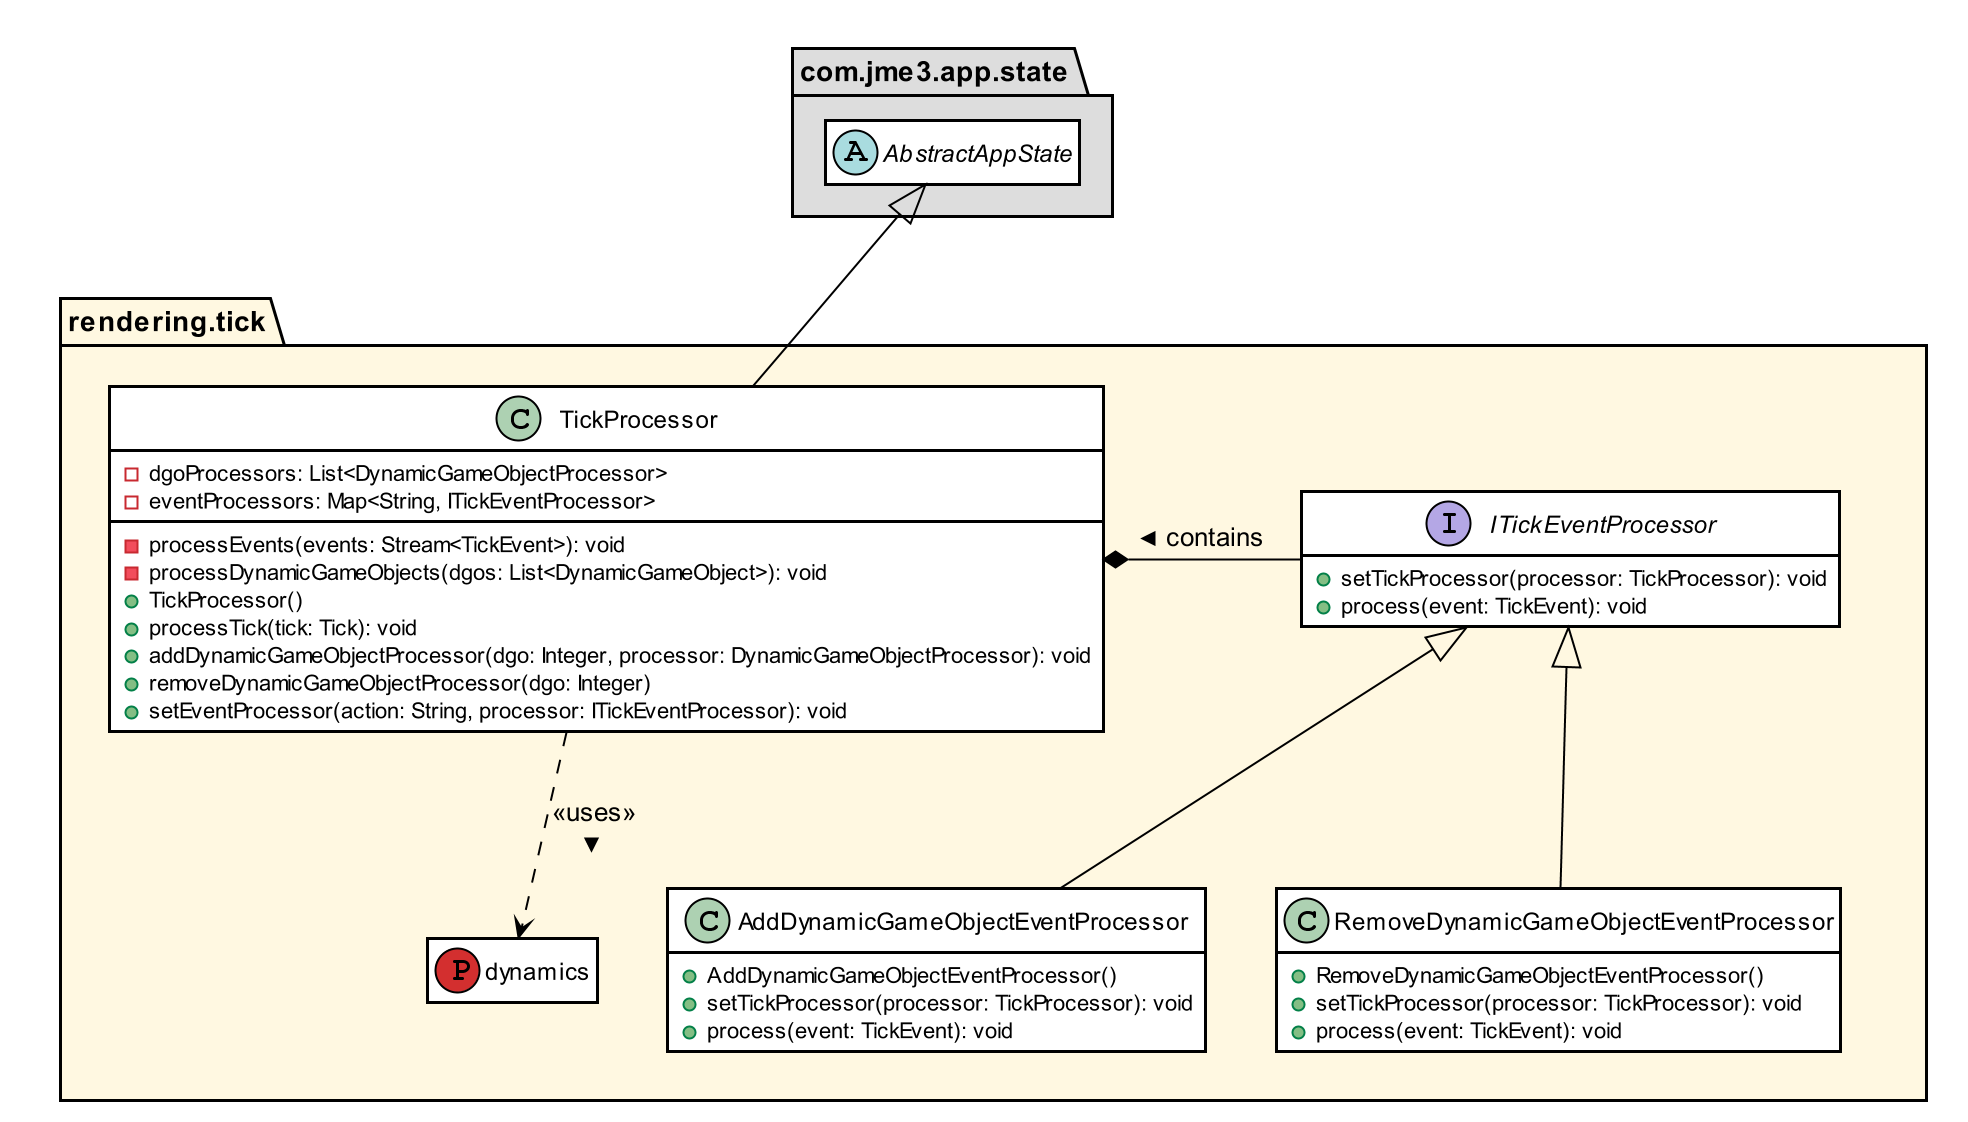
\includegraphics[width=\linewidth]{Interface/render-tick.png}
        \caption{rendering.tick Klassen-Diagram}
    \end{figure}

        \paragraph{\underline{TickProcessor}} \mbox{}\\
        \\
            Verarbeitet \textit{Tick}s indem er die in diesem enthaltenen \textit{DynamicGameObject}s an
            \textit{DynamicGameObjectProcessor}s weiterleitet und \textit{TickEvent}s mit den zugehörigen \textit{ITickEventProcessor}s bearbeitet.\par
                    
            \textbf{Attribute}
            \begin{itemize}
                \item \textit{- List<DynamicGameObjectProcessor> dgoProcessors}
                    \begin{leftbar}[0.9\linewidth]
                        Enthält alle \textit{DynamicGameObjectProcessor}s welche aktuell bekannt sind.
                    \end{leftbar}
                \item \textit{- Map<String, ITickEventProcessor> eventProcessors}
                    \begin{leftbar}[0.9\linewidth]
                        Enthält für jede bekannte Aktion eines \textit{TickEvent}s einen \textit{ITickEventProcessor}.
                    \end{leftbar}
            \end{itemize}

            \textbf{Methoden}
            \begin{itemize}
                \item  \textit{+ TickProcessor()}
                    \begin{leftbar}[0.9\linewidth]
                        Erstellt einen \textit{TickProcessor} und initialisiert dgoProcessors als leere List und eventProcessors als leere Map.
                    \end{leftbar}

                \pagebreak
                \item \textit{+ processTick(Tick tick): void}
                    \begin{leftbar}[0.9\linewidth]
                        Zunächst die \textit{TickEvent}s im gegebenen \textit{Tick} und leitet anschließend die \textit{DynamicGameObject}s
                        an die entsprechenden \textit{DynamicGameObjectProcessor}s weiter.\\
                        \textbf{@param tick} der zu bearbeitende \textit{Tick}.
                    \end{leftbar}
                \item \textit{+ addDynamicGameObjectProcessor(Integer dgo, DynamicGameObjectProcessor processor): void}
                    \begin{leftbar}[0.9\linewidth]
                        Fügt einen neuen \textit{DynamicGameObjectProcessor} für das \textit{DynamicGameObject} mit dem gegebenen index
                        zu diesem \textit{TickProcessor} hinzu.\\
                        \textbf{@param dgo} der index des \textit{DynamicGameObjects}, für welches der \textit{DynamicGameObjectProcessor} hinzugefügt werden soll.\\
                        \textbf{@param processor} der \textit{DynamicGameObjectProcessor}, welcher hinzugefügt werden soll.
                    \end{leftbar}
                \item \textit{+ removeDynamicGameObjectProcessor(int dgo): void}
                    \begin{leftbar}[0.9\linewidth]
                        Entfernt den \textit{DynamicGameObjectProcessor} des \textit{DynamicGameObject}s mit dem gegebenen index.\\
                        \textbf{@param dgo} der index des \textit{DynamicGameObjects}, dessen \textit{DynamicGameObjectProcessor} entfernt werden soll.
                    \end{leftbar}
                \item \textit{+ setEventProcessor(String action, ITickEventProcessor processor): void}
                    \begin{leftbar}[0.9\linewidth]
                        Setzt den \textit{ITickEventProcessor} welcher für \textit{TickEvent}s mit der gegebenen Aktion verwendet werden soll.\\
                        \textbf{@param action} die Aktion, für welche der \textit{ITickEventProcessor} gesetzt werden soll.\\
                        \textbf{@param processor} der \textit{ITickEventProcessor}, welcher gesetzt werden soll.
                    \end{leftbar}
            \end{itemize}

        \paragraph{\underline{ITickEventProcessor}} \mbox{}\\
        \\
            Interface welches die Funktionalität, welche benötigt ist um ein \textit{TickEvent} für den \textit{TickProcessor} zu verarbeiten, festlegt.\par

            \textbf{Methoden}					
            \begin{itemize}
                \item  \textit{+ setTickProcessor(TickProcessor processor): void}
                    \begin{leftbar}[0.9\linewidth]
                        Setzt den \textit{TickProcessor}, welcher diesen \textit{ITickEventProcessor} verwenden wird, fest.\\
                        \textbf{@param processor} der \textit{TickProcessor}, welcher diesen \textit{ITickEventProcessor} verwendet.
                    \end{leftbar}

                \pagebreak

                \item  \textit{+ process(TickEvent event): void}
                    \begin{leftbar}[0.9\linewidth]
                        Wird aufgerufen, sobald ein \textit{TickEvent} mit der Aktion, für die dieser \textit{ITickEventProcessor} registriert wurde, auftritt.\\
                        \textbf{@param event} das zu verarbeitende \textit{TickEvent}.
                    \end{leftbar}
            \end{itemize}

        \paragraph{\underline{AddDynamicGameObjectEventProcessor}} \mbox{}\\
        \\
        \textit{ITickEventProcessor} zur Bearbeitung eines \textit{TickEvent}s, welches auftritt, wenn ein neues \textit{DynamicGameObject} hinzugefügt wurde.\par

            \textbf{Attribute}
            \begin{itemize}
                \item  \textit{- TickProcessor tickProcessor}
                    \begin{leftbar}[0.9\linewidth]
                        Der \textit{TickProcessor}, welcher diesen \textit{ITickEventProcessor} verwendet.
                    \end{leftbar}
            \end{itemize}
            \textbf{Methoden}					
            \begin{itemize}
                \item  \textit{+ AddDynamicGameObjectEventProcessor()}
                    \begin{leftbar}[0.9\linewidth]
                        Erstellt einen neuen \textit{AddDynamicGameObjectEventProcessor}.
                    \end{leftbar}
                \item  \textit{+ setTickProcessor(TickProcessor processor): void}
                    \begin{leftbar}[0.9\linewidth]
                        Siehe \textit{ITickEventProcessor.setTickProcessor()}.
                    \end{leftbar}
                \item  \textit{+ process(TickEvent event): void}
                    \begin{leftbar}[0.9\linewidth]
                        Siehe \textit{ITickEventProcessor.process()}.
                    \end{leftbar}
            \end{itemize}

        \pagebreak
        \paragraph{\underline{RemoveDynamicGameObjectEventProcessor}} \mbox{}\\
        \\
        \textit{ITickEventProcessor} zur Bearbeitung eines \textit{TickEvent}s, welches auftritt, wenn \textit{DynamicGameObject} entfernt wurde.\par

            \textbf{Attribute}
            \begin{itemize}
                \item  \textit{- TickProcessor tickProcessor}
                    \begin{leftbar}[0.9\linewidth]
                        Der \textit{TickProcessor}, welcher diesen \textit{ITickEventProcessor} verwendet.
                    \end{leftbar}
            \end{itemize}
            \textbf{Methoden}					
            \begin{itemize}
                \item  \textit{+ RemoveDynamicGameObjectEventProcessor()}
                    \begin{leftbar}[0.9\linewidth]
                        Erstellt einen neuen \textit{RemoveDynamicGameObjectEventProcessor}.
                    \end{leftbar}
                \item \textit{+ setTickProcessor(TickProcessor processor): void}
                    \begin{leftbar}[0.9\linewidth]
                        Siehe \textit{ITickEventProcessor.setTickProcessor()}.
                    \end{leftbar}
                \item  \textit{+ process(TickEvent event): void}
                    \begin{leftbar}[0.9\linewidth]
                        Siehe \textit{ITickEventProcessor.process()}.
                    \end{leftbar}
            \end{itemize}
\pagebreak
\subsubsection{rendering.tick.dynamics}
    Enthält Klassen um \textit{DynamicGameObject}s auf Nodes im Scenegraph der JMonkeyEngine anzuwenden.\par

    \begin{figure}[htbp]
        \centering
        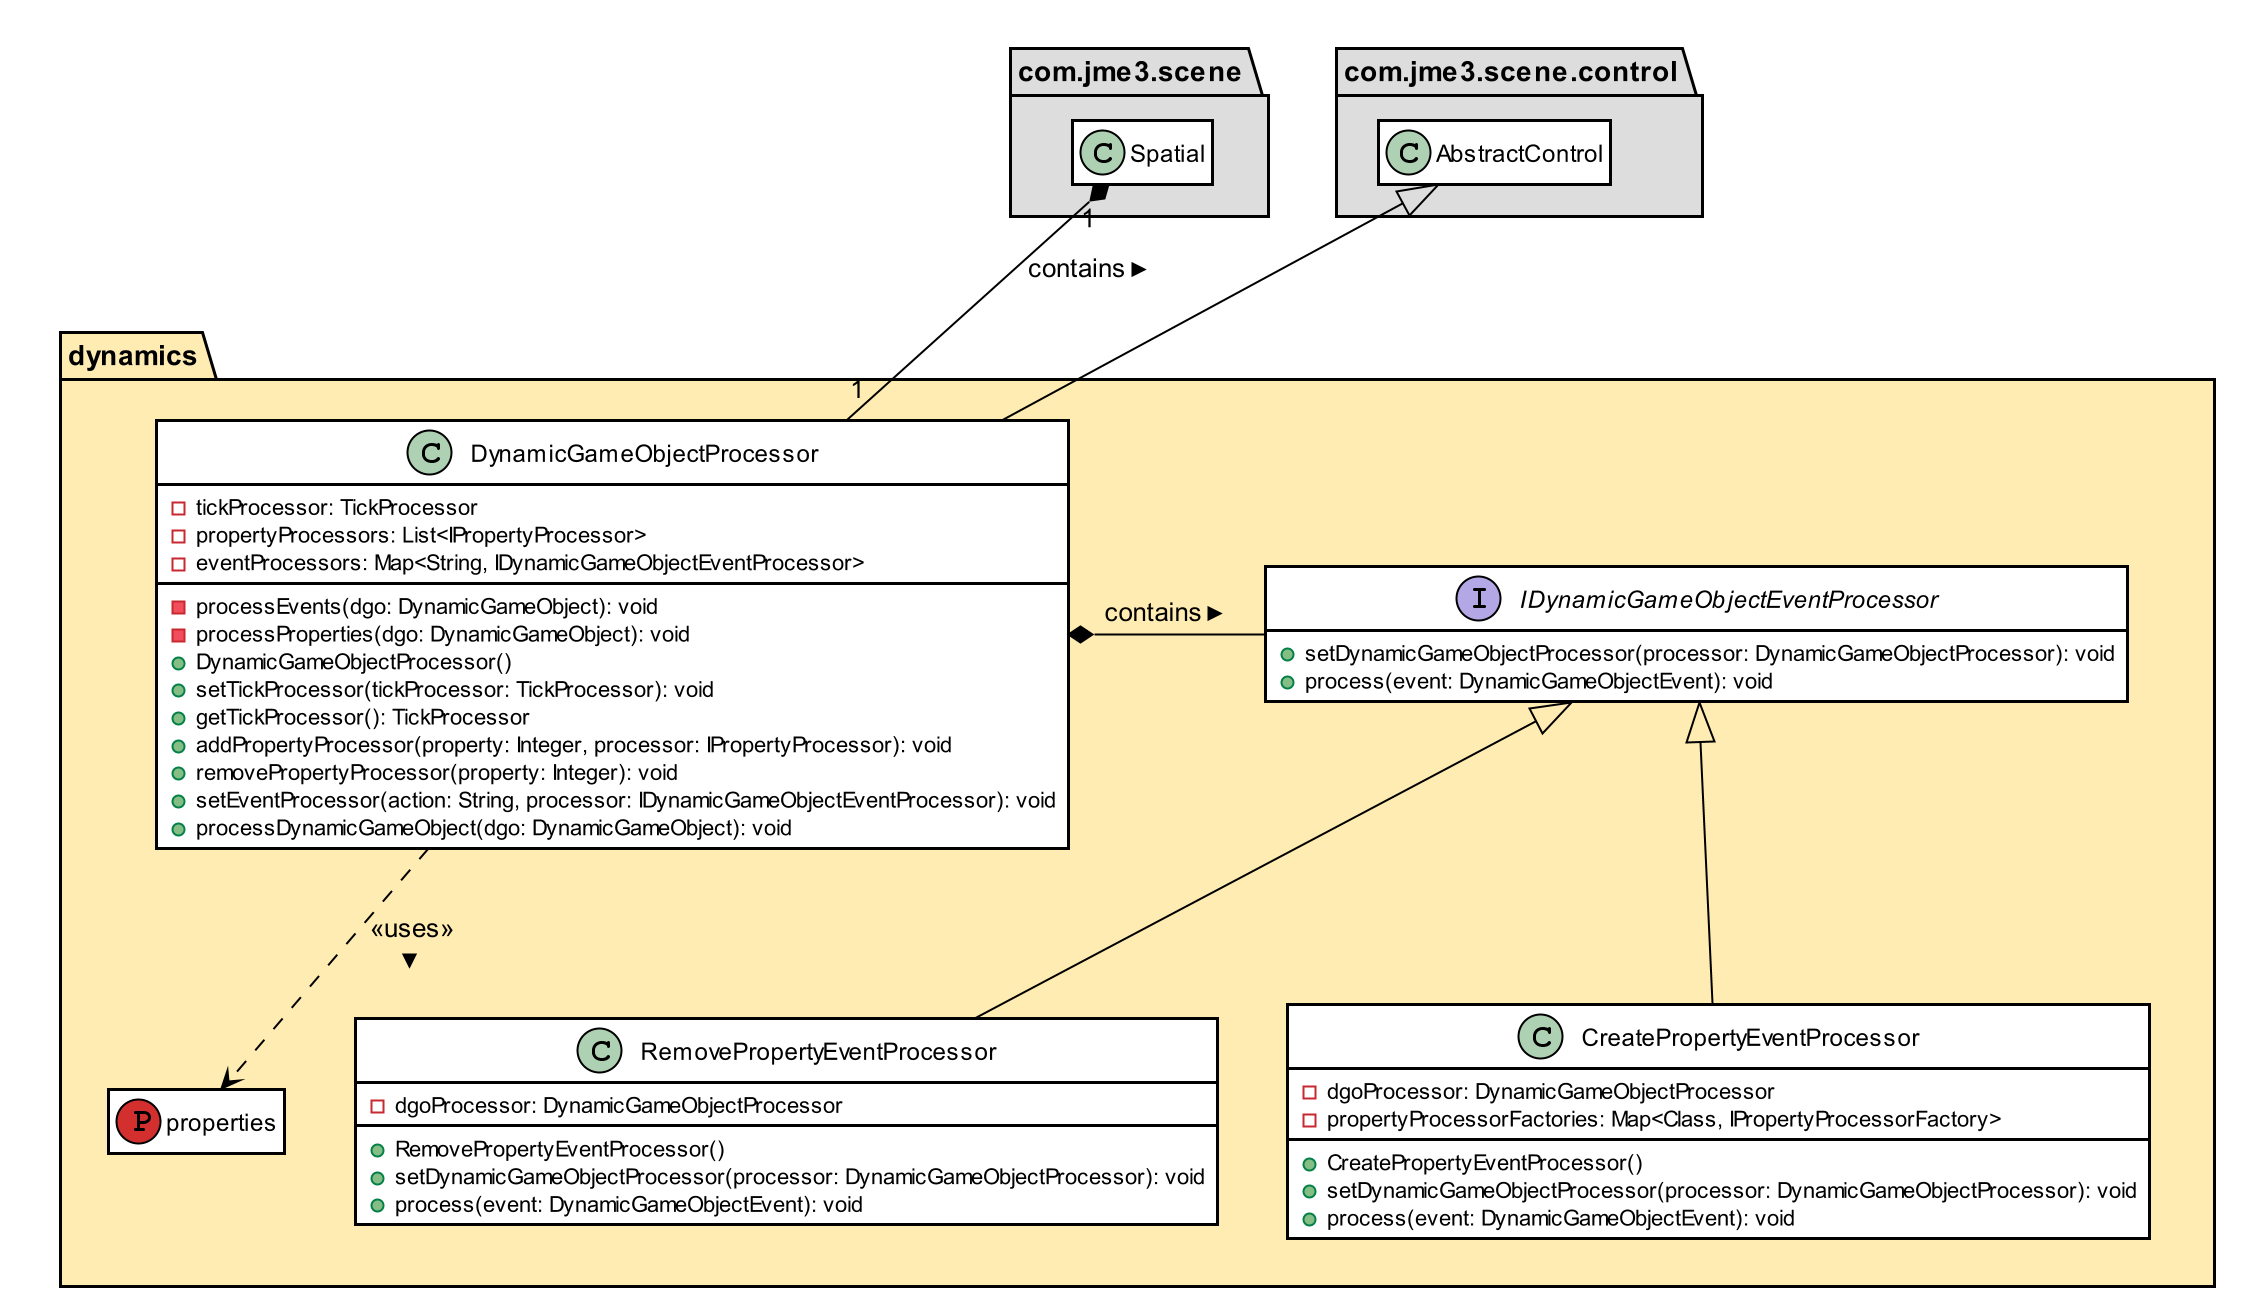
\includegraphics[width=\linewidth]{Interface/render-tick-dynamics.png}
        \caption{rendering.tick.dynamics Klassen-Diagram}
    \end{figure}

        \paragraph{\underline{DynamicGameObjectProcessor}} \mbox{}\\
        \\
            Verarbeitet \textit{DynamicGameObject}s indem er die in diesem enthaltenen \textit{IProperty}s an
            \textit{IPropertyProcessor}s weiterleitet und \textit{DynamicGameObjectEvent}s mit den zugehörigen \textit{IDynamicGameObjectEventProcessor}s bearbeitet.\par
                    
            \textbf{Attribute}
            \begin{itemize}
                \item  \textit{- TickProcessor tickProcessor}
                    \begin{leftbar}[0.9\linewidth]
                        Der \textit{TickProcessor}, welcher diesen \textit{DynamicGameObjectProcessor} verwendet.
                    \end{leftbar}
                \item \textit{- List<IPropertyProcessor> propertyProcessors}
                    \begin{leftbar}[0.9\linewidth]
                        Enthält alle momentan bekannten \textit{IPropertyProcessor}s.
                    \end{leftbar}
                \item \textit{- Map<String, IDynamicGameObjectEventProcessor> eventProcessors}
                    \begin{leftbar}[0.9\linewidth]
                        Enthält für jede benötigte Aktion eines \textit{DynamicGameObjectEvent}s einen \textit{IDynamicGameObjectEventProcessor}.
                    \end{leftbar}
            \end{itemize}

            \pagebreak
            \textbf{Methoden}
            \begin{itemize}
                \item \textit{+ DynamicGameObjectProcessor()}
                    \begin{leftbar}[0.9\linewidth]
                        Erstellt einen neuem \textit{DynamicGameObjectProcessor} und initialisiert propertyProcessors als leere List
                        und eventProcessors als leere Map.
                    \end{leftbar}
                \item \textit{+ setTickProcessor(TickProcessor tickProcessor): void}
                    \begin{leftbar}[0.9\linewidth]
                        Setzt den \textit{TickProcessor}, welcher diesen \textit{DynamicGameObjectProcessor} aufruft.\\
                        \textbf{@param tickProcessor} der \textit{TickProcessor}, welcher diesen \textit{DynamicGameObjectProcessor} aufruft.
                    \end{leftbar}
                \item \textit{+ getTickProcessor(): TickProcessor}
                    \begin{leftbar}[0.9\linewidth]
                        \textbf{@return} den \textit{TickProcessor}, welcher diesen \textit{DynamicGameObjectProcessor} aufruft.
                    \end{leftbar}
                \item \textit{+ addPropertyProcessor(int property, IPropertyProcessor processor): void}
                    \begin{leftbar}[0.9\linewidth]
                        Fügt einen \textit{IPropertyProcessor} für die \textit{IProperty} mit dem gegebenen index hinzu.\\
                        \textbf{@param property} der index der \textit{IProperty}.\\
                        \textbf{@param processor} der \textit{IPropertyProcessor}, wecher hinzugefügt werden soll.
                    \end{leftbar}
                \item \textit{+ removePropertyProcessor(int property): void}
                    \begin{leftbar}[0.9\linewidth]
                        Entfernt \textit{IPropertyProcessor} für die \textit{IProperty} mit dem gegebenen index.\\
                        \textbf{@param property} der index der \textit{IProperty}.
                    \end{leftbar}
                \item \textit{+ setEventProcessor(String action, IDynamicGameObjectEventProcessor processor): void}
                    \begin{leftbar}[0.9\linewidth]
                        Setzt den \textit{IDynamicGameObjectEvenProcessor} für \textit{DynamicGameObjectEvent}s mit der gegebenen Aktion.\\
                        \textbf{@param action} die Aktion für die der \textit{IDynamicGameObjectEvenProcessor} gesetzt werden soll.
                        \textbf{@param processor} der \textit{IDynamicGameObjectEvenProcessor}
                    \end{leftbar}
                \item \textit{+ processBundle(DynamicGameObject dgo): void}
                    \begin{leftbar}[0.9\linewidth]
                        Verarbeitet das gegebene \textit{DynamicGameObject}.\\
                        \textbf{@param dgo} das \textit{DynamicGameObject}, das verarbeitet werden soll.
                    \end{leftbar}
            \end{itemize}

        \paragraph{\underline{IDynamicGameObjectEventProcessor}} \mbox{}\\
        \\
            Wird von einem \textit{DynamicGameObjectProcessor} verwendet, um \textit{DynamicGameObjectEvent}s zu verarbeiten.\par

            \pagebreak
            \textbf{Methoden}
            \begin{itemize}
                \item \textit{+ setBundleProcessor(DynamicGameObjectProcessor processor): void}
                    \begin{leftbar}[0.9\linewidth]
                        Setzt den \textit{DynamicGameObjectProcessor}, welcher diesen \textit{IDynamicGameObjectEventProcessor} verwendet.\\
                        \textbf{@param processor} der \textit{DynamicsGameProcessor}.
                    \end{leftbar}
                \item \textit{+ process(DynamicGameObjectEvent event): void}
                    \begin{leftbar}[0.9\linewidth]
                        Verarbeitet das gegebene \textit{DynamicGameObjectEvent}.\\
                        \textbf{@param event} das \textit{DynamicGameObjectEvent}.
                    \end{leftbar}
            \end{itemize}

        \paragraph{\underline{CreatePropertyEventProcessor}} \mbox{}\\
        \\
        \textit{IDynamicGameObjectEventProcessor}, zur Verarbeitung von \textit{DynamicGameObjectEvent}s, welche auftreten wenn eine \textit{IProperty} hinzugefügt wurde.

            \textbf{Attribute}
            \begin{itemize}
                \item  \textit{- DynamicGameObjectProcessor dgoProcessor}
                    \begin{leftbar}[0.9\linewidth]
                        Der \textit{DynamicGameObjectProcessor}, welcher diesen \textit{IDynamicGameObjectEventProcessor} verwendet.
                    \end{leftbar}
            \end{itemize}
            \textbf{Methoden}
            \begin{itemize}
                \item \textit{+ setBundleProcessor(DynamicGameObjectProcessor processor): void}
                    \begin{leftbar}[0.9\linewidth]
                        Siehe \textit{IDynamicGameObjectEventProcessor.setBundleProcessor()}.
                    \end{leftbar}
                \item \textit{+ process(DynamicGameObjectEvent event): void}
                    \begin{leftbar}[0.9\linewidth]
                        Siehe \textit{IDynamicGameObjectEventProcessor.process()}.
                    \end{leftbar}
            \end{itemize}
        
        \pagebreak
        \paragraph{\underline{RemovePropertyEventProcessor}} \mbox{}\\
        \\
        \textit{IDynamicGameObjectEventProcessor}, zur Verarbeitung von \textit{DynamicGameObjectEvent}s, welche auftreten wenn eine \textit{IProperty} entfernt wurde.

            \textbf{Attribute}
            \begin{itemize}
                \item  \textit{- DynamicGameObjectProcessor dgoProcessor}
                    \begin{leftbar}[0.9\linewidth]
                        Der \textit{DynamicGameObjectProcessor}, welcher diesen \textit{IDynamicGameObjectEventProcessor} verwendet.
                    \end{leftbar}
            \end{itemize}
            \textbf{Methoden}
            \begin{itemize}
                \item \textit{+ setBundleProcessor(processor: DynamicGameObjectProcessor): void}
                    \begin{leftbar}[0.9\linewidth]
                        Siehe \textit{IDynamicGameObjectEventProcessor.setBundleProcessor()}.
                    \end{leftbar}
                \item \textit{+ process(DynamicGameObjectEvent event): void}
                    \begin{leftbar}[0.9\linewidth]
                        Siehe \textit{IDynamicGameObjectEventProcessor.process()}.
                    \end{leftbar}
            \end{itemize}
\pagebreak
\subsubsection{rendering.tick.dynamics.properties}
Enthält Klassen für die Verarbeitung von \textit{IProperty}s

    \begin{figure}[htbp]
        \centering
        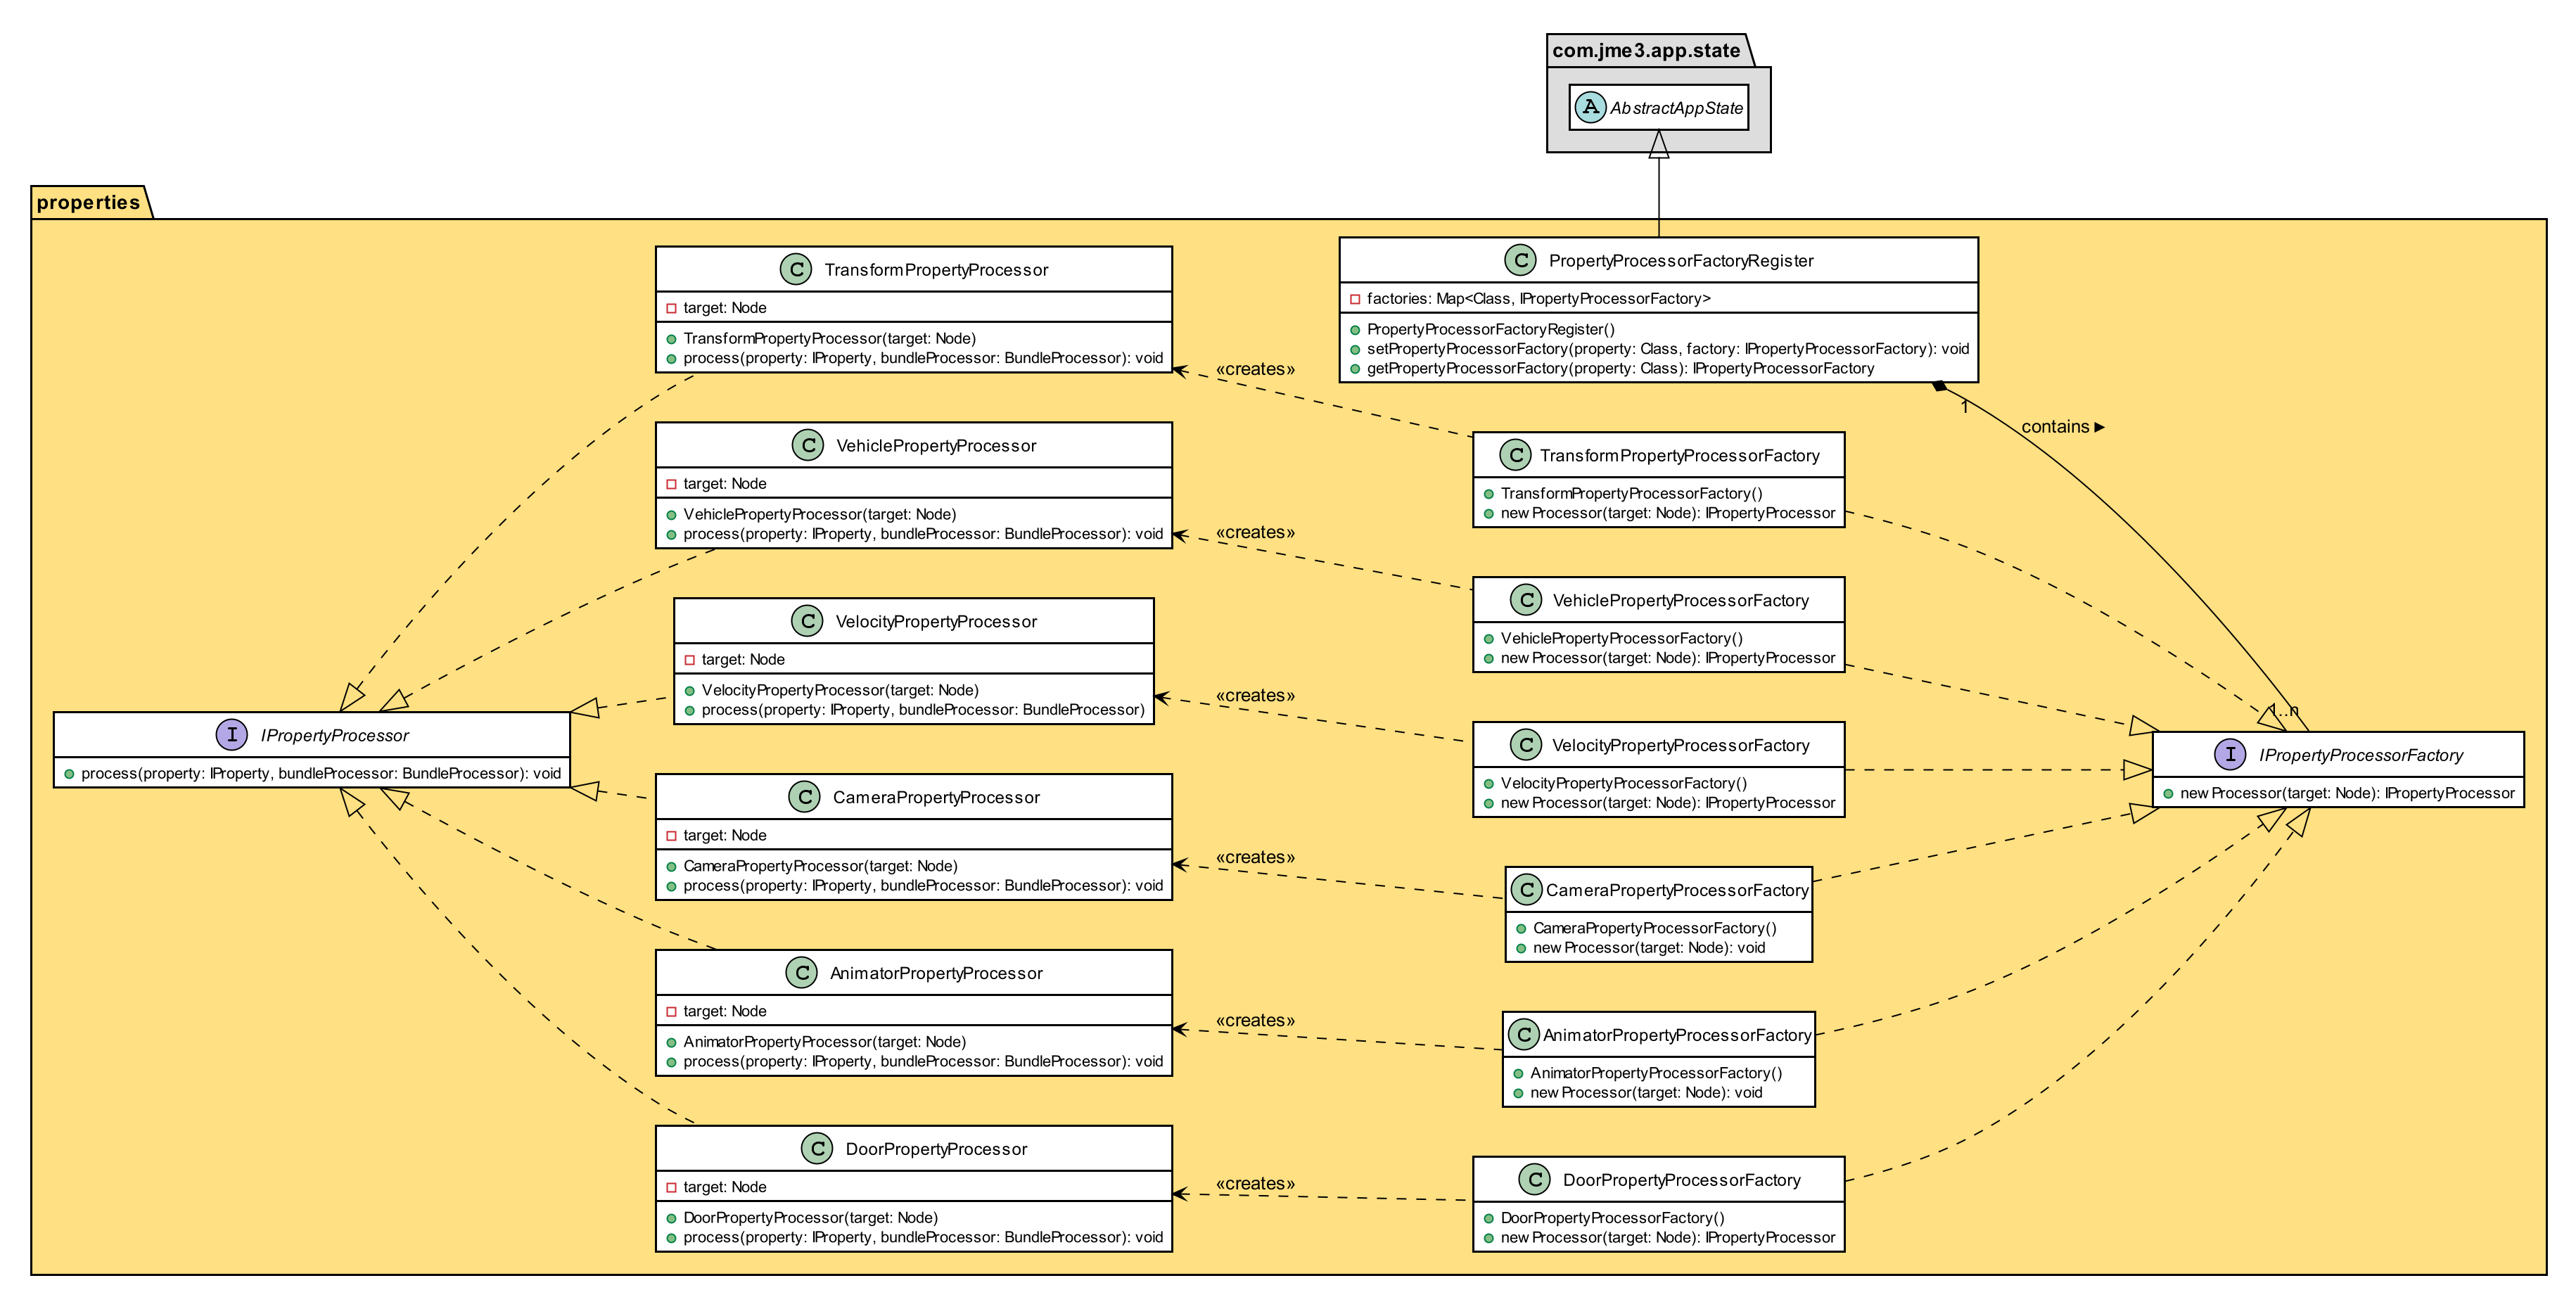
\includegraphics[width=0.9\linewidth]{Interface/render-tick-dynamics-properties.png}
        \caption{rendering.tick.dynamics.properties Klassen-Diagram}
    \end{figure}

    \paragraph{\underline{IPropertyProcessor}} \mbox{}\\
    \\
    Interface welches die Funktionalität für die Verarbeitung von \textit{IProperty}s.\par

        \textbf{Methoden}
        \begin{itemize}
            \item  \textit{+ process(IProperty property, DynamicGameObjectProcessor dgoProcessor): void}
                \begin{leftbar}[0.9\linewidth]
                    Verarbeitet die gegebene \textit{IProperty}.\\
                    \textbf{@param property} die \textit{IProperty} welche verarbeitet werden soll.\\
                    \textbf{@param dgoProcessor} der \textit{DynamicGameObjectProcessor} welcher die Methode aufgerufen hat.\\
                    \textbf{@throws IllegalStateException} falls die gegebene \textit{IProperty} nicht von diesem \textit{IPropertyProcessor}
                    bearbeitet werden kann.
                \end{leftbar}
        \end{itemize}

    \pagebreak
    \paragraph{\underline{IPropertyProcessorFactory}} \mbox{}\\
    \\
    Interface für Fabriken von \textit{IPropertyProcessor}s.\par

        \textbf{Methoden}
        \begin{itemize}
            \item \textit{+ newProcessor(Node target): IPropertyProcessor}
                \begin{leftbar}[0.9\linewidth]
                    Erstellt einen neuen \textit{IPropertyProcessor} welcher auf der gegebenen \textit{Node} arbeitet.\\
                    \textbf{@param target} die \textit{Node}, auf welcher der \textit{IPropertyProcessor} arbeiten soll.
                    \textbf{@return} der neu erstellte \textit{IPropertyProcessor}.
                \end{leftbar}
        \end{itemize}

    \paragraph{\underline{TransformPropertyProcessor}} \mbox{}\\
    \\
    \textit{IPropertyProcessor} für \textit{TransformProperty}s.\par

        \textbf{Attribute}
        \begin{itemize}
            \item \textit{+ Node target}
                \begin{leftbar}[0.9\linewidth]
                    Die \textit{Node} auf welcher dieser \textit{TransformPropertyProcessor} arbeitet.
                \end{leftbar}
        \end{itemize}
        \textbf{Methoden}
        \begin{itemize}
            \item \textit{+ TransformPropertyProcessor(Node target)}
                \begin{leftbar}[0.9\linewidth]
                    Erstellt einen neuen \textit{TransformPropertyProcessor}.\\
                    \textbf{@param target} die \textit{Node} auf welcher dieser \textit{TransformPropertyProcessor} arbeitet.
                \end{leftbar}
            \item \textit{+ process(IProperty property, DynamicGameObjectProcessor dgoProcessor): void}
                \begin{leftbar}[0.9\linewidth]
                    Siehe \textit{IPropertyProcessor.process()}.
                \end{leftbar}
        \end{itemize}

    \paragraph{\underline{TransformPropertyProcessorFactory}} \mbox{}\\
    \\
    Fabrik für \textit{TransformPropertyProcessor}s.\par

        \textbf{Methoden}
        \begin{itemize}
            \item \textit{+ TransformPropertyProcessorFactory()}
                \begin{leftbar}[0.9\linewidth]
                    Erstellt eine neue \textit{TransformPropertyProcessorFactory}.
                \end{leftbar}
            \item \textit{+ newProcessor(Node target): IPropertyProcessor}
                \begin{leftbar}[0.9\linewidth]
                    Siehe \textit{IPropertyProcessorFactory.newProcessor()}.
                \end{leftbar}
        \end{itemize}

    \paragraph{\underline{VelocityPropertyProcessor}} \mbox{}\\
    \\
    \textit{IPropertyProcessor} für \textit{VelocityProperty}s.\par

        \textbf{Attribute}
        \begin{itemize}
            \item \textit{+ Node target}
                \begin{leftbar}[0.9\linewidth]
                    Die \textit{Node} auf welcher dieser \textit{VelocityPropertyProcessor} arbeitet.
                \end{leftbar}
        \end{itemize}
        \textbf{Methoden}
        \begin{itemize}
            \item \textit{+ VelocityPropertyProcessor(Node target)}
                \begin{leftbar}[0.9\linewidth]
                    Erstellt einen neuen \textit{VelocityPropertyProcessor}.\\
                    \textbf{@param target} die \textit{Node} auf welcher dieser \textit{VelocityPropertyProcessor} arbeitet.
                \end{leftbar}
            \item \textit{+ process(IProperty property, DynamicGameObjectProcessor dgoProcessor): void}
                \begin{leftbar}[0.9\linewidth]
                    Siehe \textit{IPropertyProcessor.process()}.
                \end{leftbar}
        \end{itemize}

    \paragraph{\underline{VelocityPropertyProcessorFactory}} \mbox{}\\
    \\
    Fabrik für \textit{VelocityPropertyProcessor}s.\par

        \textbf{Methoden}
        \begin{itemize}
            \item \textit{+ VelocityPropertyProcessorFactory()}
                \begin{leftbar}[0.9\linewidth]
                    Erstellt eine neue \textit{VelocityPropertyProcessorFactory}.
                \end{leftbar}
            \item \textit{+ newProcessor(Node target): IPropertyProcessor}
                \begin{leftbar}[0.9\linewidth]
                    Siehe \textit{IPropertyProcessorFactory.newProcessor()}.
                \end{leftbar}
        \end{itemize}

    \paragraph{\underline{CameraPropertyProcessor}} \mbox{}\\
    \\
    \textit{IPropertyProcessor} für \textit{CameraProperty}s.\par

        \textbf{Attribute}
        \begin{itemize}
            \item \textit{+ Node target}
                \begin{leftbar}[0.9\linewidth]
                    Die \textit{Node} auf welcher dieser \textit{CameraPropertyProcessor} arbeitet.
                \end{leftbar}
        \end{itemize}

        \pagebreak
        \textbf{Methoden}
        \begin{itemize}
            \item \textit{+ CameraPropertyProcessor(Node target)}
                \begin{leftbar}[0.9\linewidth]
                    Erstellt einen neuen \textit{CameraPropertyProcessor}.\\
                    \textbf{@param target} die \textit{Node} auf welcher dieser \textit{CameraPropertyProcessor} arbeitet.
                \end{leftbar}
            \item \textit{+ process(IProperty property, DynamicGameObjectProcessor dgoProcessor): void}
                \begin{leftbar}[0.9\linewidth]
                    Siehe \textit{IPropertyProcessor.process()}.
                \end{leftbar}
        \end{itemize}

    \paragraph{\underline{CameraPropertyProcessorFactory}} \mbox{}\\
    \\
    Fabrik für \textit{CameraPropertyProcessor}s.\par

        \textbf{Methoden}
        \begin{itemize}
            \item \textit{+ CameraPropertyProcessorFactory()}
                \begin{leftbar}[0.9\linewidth]
                    Erstellt eine neue \textit{CameraPropertyProcessorFactory}.
                \end{leftbar}
            \item \textit{+ newProcessor(Node target): IPropertyProcessor}
                \begin{leftbar}[0.9\linewidth]
                    Siehe \textit{IPropertyProcessorFactory.newProcessor()}.
                \end{leftbar}
        \end{itemize}

    \paragraph{\underline{VehiclePropertyProcessor}} \mbox{}\\
    \\
    \textit{IPropertyProcessor} für \textit{VehicleProperty}s.\par

        \textbf{Attribute}
        \begin{itemize}
            \item \textit{+ Node target}
                \begin{leftbar}[0.9\linewidth]
                    Die \textit{Node} auf welcher dieser \textit{VehiclePropertyProcessor} arbeitet.
                \end{leftbar}
        \end{itemize}
        \textbf{Methoden}
        \begin{itemize}
            \item \textit{+ VehiclePropertyProcessor(Node target)}
                \begin{leftbar}[0.9\linewidth]
                    Erstellt einen neuen \textit{VehiclePropertyProcessor}.\\
                    \textbf{@param target} die \textit{Node} auf welcher dieser \textit{VehiclePropertyProcessor} arbeitet.
                \end{leftbar}
            \item \textit{+ process(IProperty property, DynamicGameObjectProcessor dgoProcessor): void}
                \begin{leftbar}[0.9\linewidth]
                    Siehe \textit{IPropertyProcessor.process()}.
                \end{leftbar}
        \end{itemize}

    \pagebreak
    \paragraph{\underline{VehiclePropertyProcessorFactory}} \mbox{}\\
    \\
    Fabrik für \textit{VehiclePropertyProcessor}s.\par

        \textbf{Methoden}
        \begin{itemize}
            \item \textit{+ VehiclePropertyProcessorFactory()}
                \begin{leftbar}[0.9\linewidth]
                    Erstellt eine neue \textit{VehiclePropertyProcessorFactory}.
                \end{leftbar}
            \item \textit{+ newProcessor(Node target): IPropertyProcessor}
                \begin{leftbar}[0.9\linewidth]
                    Siehe \textit{IPropertyProcessorFactory.newProcessor()}.
                \end{leftbar}
        \end{itemize}

    \paragraph{\underline{AnimatorPropertyProcessor}} \mbox{}\\
    \\
    \textit{IPropertyProcessor} für \textit{AnimatorProperty}s.\par

        \textbf{Attribute}
        \begin{itemize}
            \item \textit{+ Node target}
                \begin{leftbar}[0.9\linewidth]
                    Die \textit{Node} auf welcher dieser \textit{AnimatorPropertyProcessor} arbeitet.
                \end{leftbar}
        \end{itemize}
        \textbf{Methoden}
        \begin{itemize}
            \item \textit{+ AnimatorPropertyProcessor(Node target)}
                \begin{leftbar}[0.9\linewidth]
                    Erstellt einen neuen \textit{AnimatorPropertyProcessor}.\\
                    \textbf{@param target} die \textit{Node} auf welcher dieser \textit{AnimatorPropertyProcessor} arbeitet.
                \end{leftbar}
            \item \textit{+ process(IProperty property, DynamicGameObjectProcessor dgoProcessor): void}
                \begin{leftbar}[0.9\linewidth]
                    Siehe \textit{IPropertyProcessor.process()}.
                \end{leftbar}
        \end{itemize}

    \paragraph{\underline{AnimatorPropertyProcessorFactory}} \mbox{}\\
    \\
    Fabrik für \textit{AnimatorPropertyProcessor}s.\par

        \textbf{Methoden}
        \begin{itemize}
            \item \textit{+ AnimatorPropertyProcessorFactory()}
                \begin{leftbar}[0.9\linewidth]
                    Erstellt eine neue \textit{AnimatorPropertyProcessorFactory}.
                \end{leftbar}
            \item \textit{+ newProcessor(Node target): IPropertyProcessor}
                \begin{leftbar}[0.9\linewidth]
                    Siehe \textit{IPropertyProcessorFactory.newProcessor()}.
                \end{leftbar}
        \end{itemize}

    \pagebreak
    \paragraph{\underline{DoorPropertyProcessor}} \mbox{}\\
    \\
    \textit{IPropertyProcessor} für \textit{DoorProperty}s.\par

        \textbf{Attribute}
        \begin{itemize}
            \item \textit{+ Node target}
                \begin{leftbar}[0.9\linewidth]
                    Die \textit{Node} auf welcher dieser \textit{DoorPropertyProcessor} arbeitet.
                \end{leftbar}
        \end{itemize}
        \textbf{Methoden}
        \begin{itemize}
            \item \textit{+ DoorPropertyProcessor(Node target)}
                \begin{leftbar}[0.9\linewidth]
                    Erstellt einen neuen \textit{DoorPropertyProcessor}.\\
                    \textbf{@param target} die \textit{Node} auf welcher dieser \textit{DoorPropertyProcessor} arbeitet.
                \end{leftbar}
            \item \textit{+ process(IProperty property, DynamicGameObjectProcessor dgoProcessor): void}
                \begin{leftbar}[0.9\linewidth]
                    Siehe \textit{IPropertyProcessor.process()}.
                \end{leftbar}
        \end{itemize}

    \paragraph{\underline{DoorPropertyProcessorFactory}} \mbox{}\\
    \\
    Fabrik für \textit{DoorPropertyProcessor}s.\par

        \textbf{Methoden}
        \begin{itemize}
            \item \textit{+ DoorPropertyProcessorFactory()}
                \begin{leftbar}[0.9\linewidth]
                    Erstellt eine neue \textit{DoorPropertyProcessorFactory}.
                \end{leftbar}
            \item \textit{+ newProcessor(Node target): IPropertyProcessor}
                \begin{leftbar}[0.9\linewidth]
                    Siehe \textit{IPropertyProcessorFactory.newProcessor()}.
                \end{leftbar}
        \end{itemize}

    \pagebreak
    \paragraph{\underline{PropertyProcessorFactoryRegister}} \mbox{}\\
    \\
    \textit{Appstate}, welcher alls bekannten \textit{IPropertyProcessorFactory}s hält.\par

        \textbf{Methoden}
        \begin{itemize}
            \item \textit{+ PropertyProcessorFactoryRegister()}
                \begin{leftbar}[0.9\linewidth]
                    Erstellt ein neues \textit{PropertyProcessorFactoryRegister} und initialisiert factories als leere Map.
                \end{leftbar}
            \item \textit{+ setPropertyProcessorFactory(Class<? extends IProperty> property, IPropertyProcessorFactory factory): void}
                \begin{leftbar}[0.9\linewidth]
                    Setzt die \textit{IPropertyProcessorFactory}, welche verwendet wird um \textit{IPropertyProcessor}s für eine \textit{IProperty} vom gegebenen Typ
                    zu erstellen.\\
                    \textbf{@param property} der Typ von \textit{IProperty} für den diese \textit{IPropertyProcessorFactory} verwendet werden soll.\\
                    \textbf{@param factory} die \textit{IPropertyProcessorFactory}.
                \end{leftbar}
            \item \textit{+ getPropertyProcessorFactory(Class<? extends IProperty> property): IPropertyProcessorFactory}
                \begin{leftbar}[0.9\linewidth]
                    Liefert die \textit{IPropertyProcessorFactory}, welche für den gegebenen Typ von \textit{IProperty} verwendet werden soll.\\
                    \textbf{@param property} der Typ von \textit{IProperty} für den die \textit{IPropertyProcessorFactory} gesucht ist.\\
                    \textbf{@return} die \textit{IPropertyProcessorFactory} für den gegebenen Typ von \textit{IProperty} oder null falls keine
                    \textit{IPropertyProcessorFactory} für diesen Typ gesetzt wurde.
                \end{leftbar}
        \end{itemize}
\pagebreak
		\subsection{Assets}

\subsubsection{assets}

    Enthält Funktionalität zum asynchronen laden von Assets.

    \begin{figure}[htbp]
        \centering
        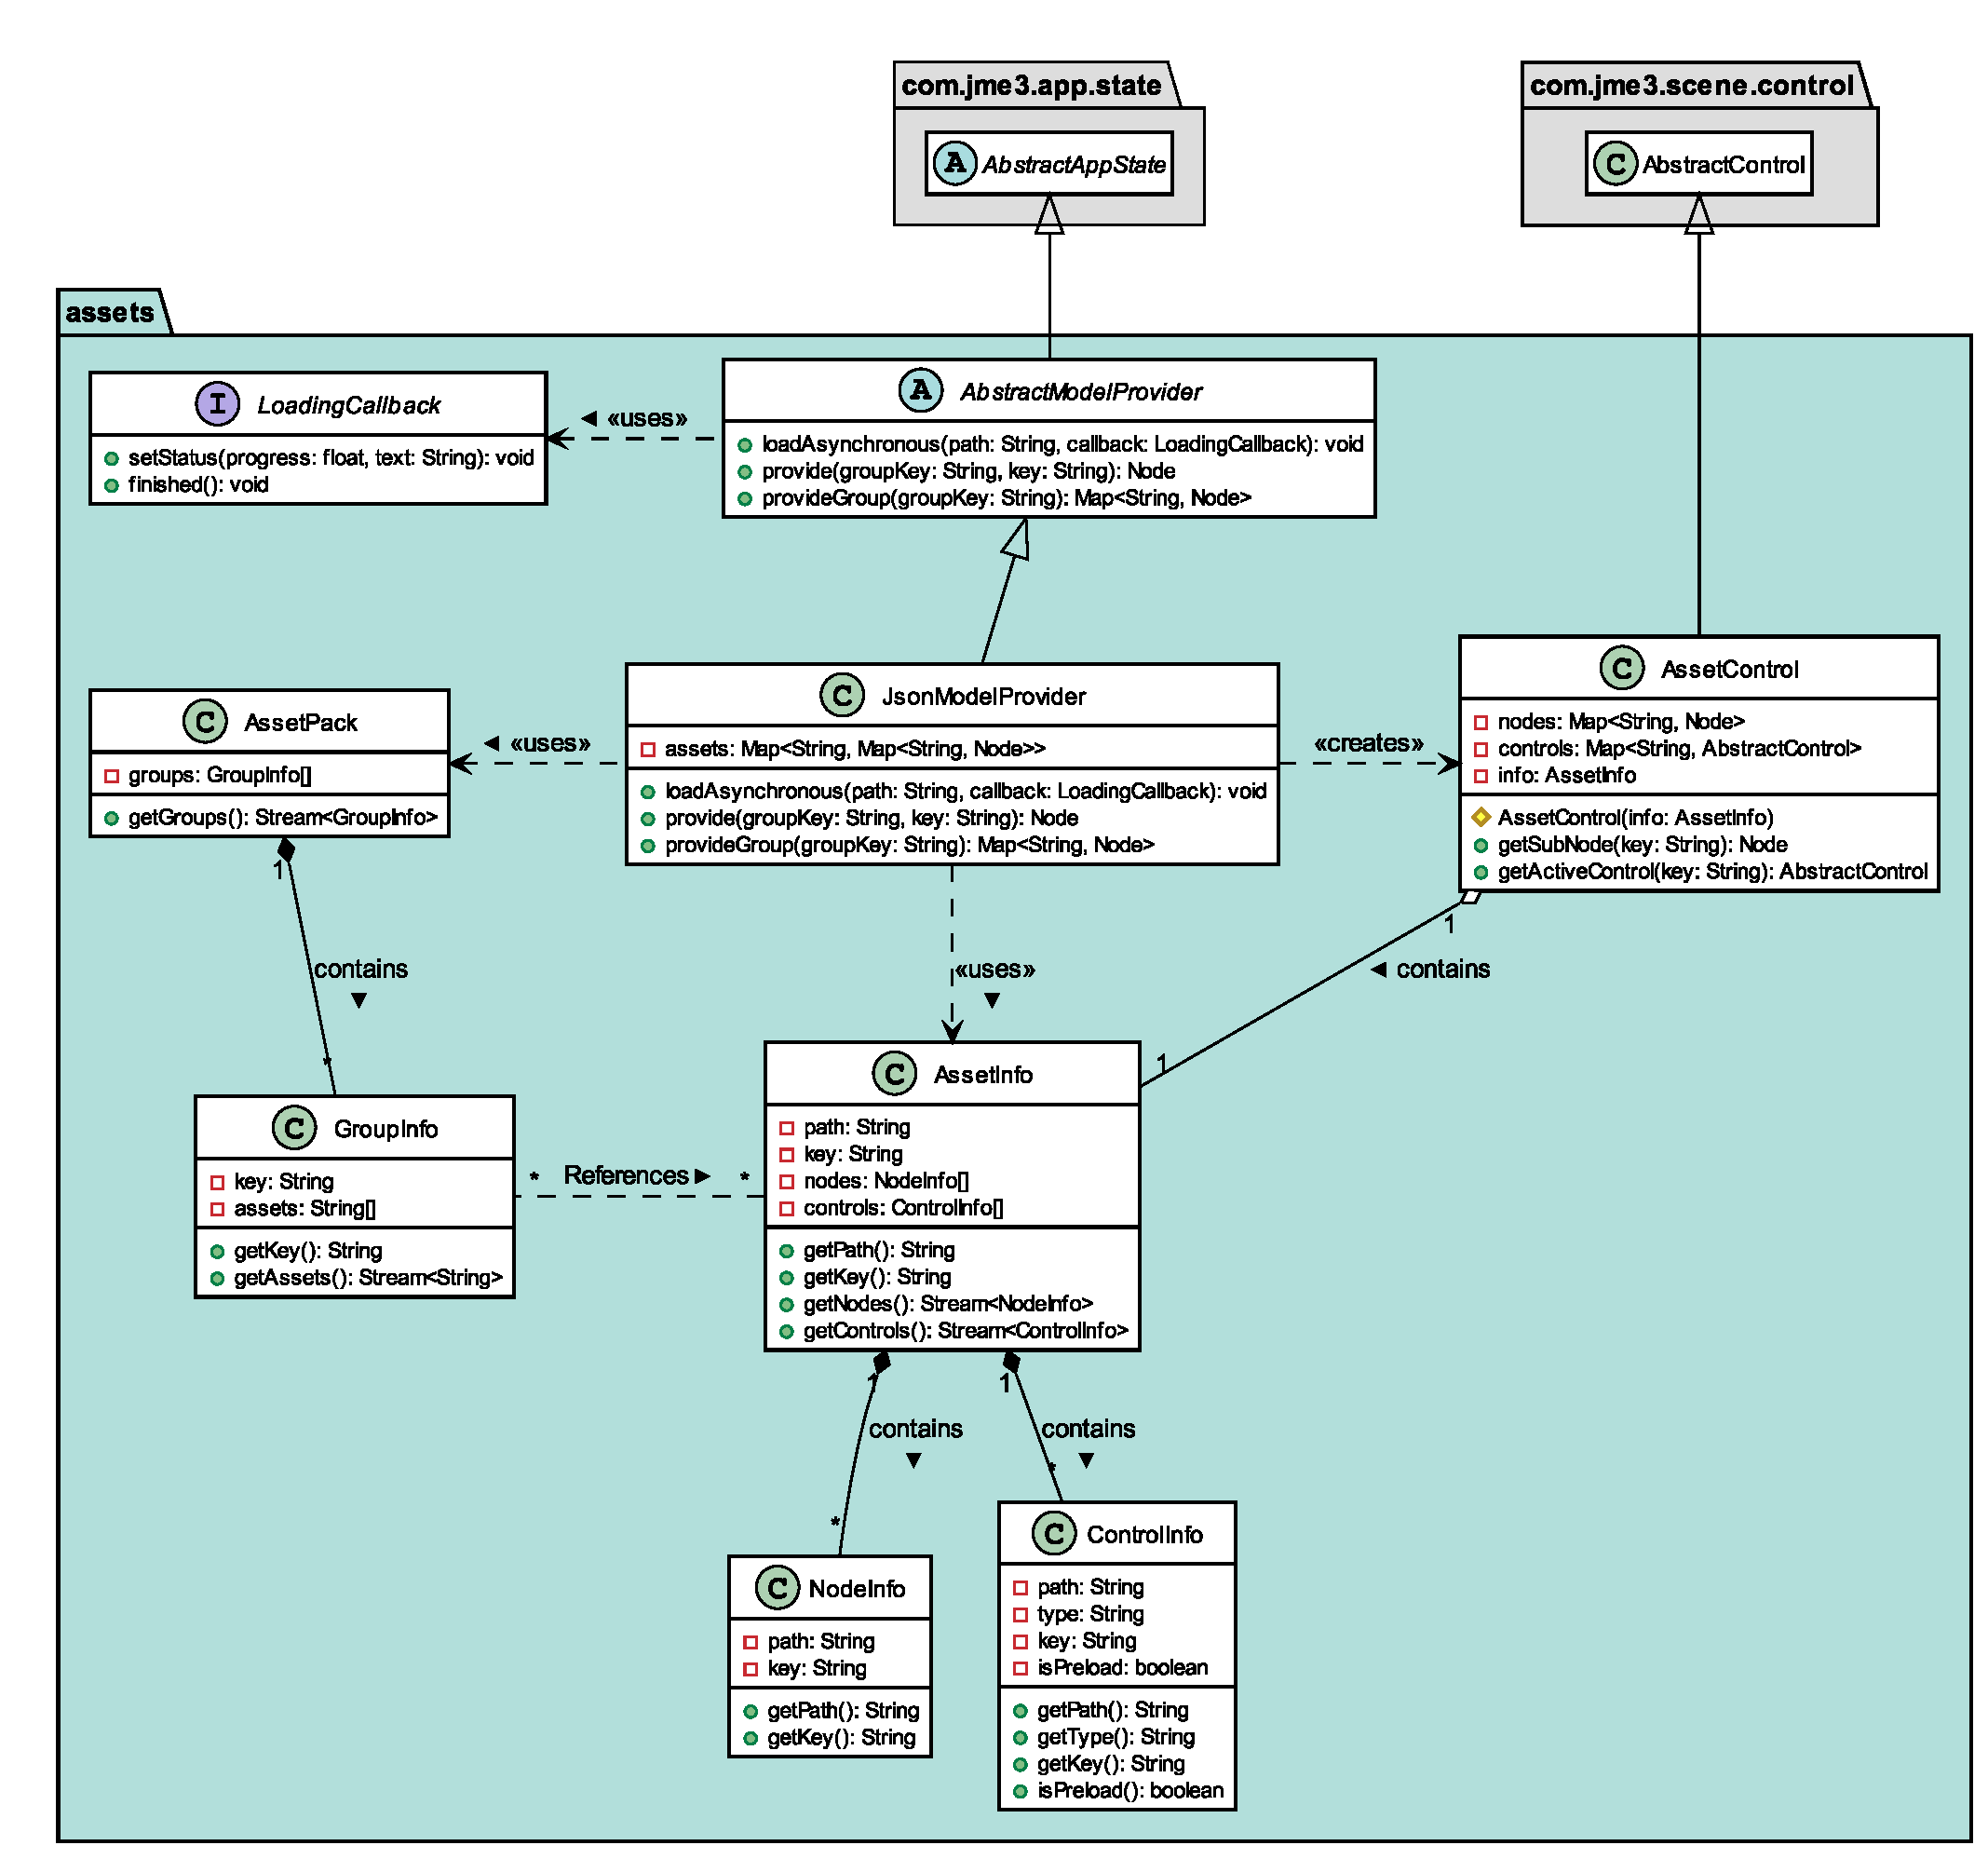
\includegraphics[width=\linewidth]{Assets/assets.eps}
        \caption{assets Klassen-Diagram}
    \end{figure}

    \pagebreak
    \paragraph{\underline{AbstractModelProvider}} \mbox{}\\
    \\
        Ein Appstate, welcher funktionalität zum laden von Assets definiert.\par

        \textbf{Methoden}
        \begin{itemize}
            \item \textit{+ loadAsynchronous(String path, LoadingCallback callback)}
                \begin{leftbar}[0.9\linewidth]
                    Lädt das \textit{AssetPack} am gegebenen Pfad in einem neuen Thread.\\
                    \textbf{@param path} Der Pfad zum \textit{AssetPack}, welches geladen werden soll.\\
                    \textbf{@param callback} Das \textit{LoadingCallback}, welches verwendet wird um dem Ladebildschirm den Status mitzuteilen.
                \end{leftbar}
            \item \textit{+ provide(String groupKey, String key): Node}
                \begin{leftbar}[0.9\linewidth]
                    Gibt ein Asset zurück.\\
                    \textbf{@param groupKey} Der Name der Gruppe zu der das Asset gehört.\\
                    \textbf{@param key} Der Name des Assets.
                \end{leftbar}
            \item \textit{+ provideGroup(String groupKey): Map<String, Node>}
                \begin{leftbar}[0.9\linewidth]
                    Gibt eine Gruppe von Assets zurück.\\
                    \textbf{@param groupKey} Der Name der Gruppe.
                \end{leftbar}
        \end{itemize}

    \paragraph{\underline{JsonModelProvider}} \mbox{}\\
    \\
        Ein \textit{AbstractModelProvider}, welcher \textit{AssetPack}s aus .json Dateien Lädt.\par

        \textbf{Attribute}
        \begin{itemize}
            \item \textit{- Map<String, Map<String, Node>> assets}
                \begin{leftbar}[0.9\linewidth]
                   Enthält alle Gruppen von Assets mit ihren Assets.
                \end{leftbar}
        \end{itemize}
        \textbf{Methoden}
        \begin{itemize}
            \item \textit{+ loadAsynchronous(String path, LoadingCallback callback)}
                \begin{leftbar}[0.9\linewidth]
                   Siehe \textit{AbstractModelProvider.loadAsynchronous()}.
                \end{leftbar}
            \item \textit{+ provide(String groupKey, String key): Node}
                \begin{leftbar}[0.9\linewidth]
                    Siehe \textit{AbstractModelProvider.provide()}.
                \end{leftbar}
            \item \textit{+ provideGroup(String groupKey): Map<String, Node>}
                \begin{leftbar}[0.9\linewidth]
                    Siehe \textit{AbstractModelProvider.provideGroup()}.
                \end{leftbar}
        \end{itemize}

    \paragraph{\underline{LoadingCallback}} \mbox{}\\
    \\
        Definiert die Schnittstelle, welche vom \textit{AbstractModelProvider} verwendet wird, um dem Ladebildschirm den Status mitzuteilen.\par

        \textbf{Methoden}
        \begin{itemize}
            \item \textit{+ setStatus(float progress, String text): void}
                \begin{leftbar}[0.9\linewidth]
                   Setzt den Status im Ladebildschirm.\\
                   \textbf{@param progress} der Fortschritt beim Laden.\\
                   \textbf{@param text} der Text der auf dem Ladebildschirm angezeigt werden soll.
                \end{leftbar}
            \item \textit{+ finished(): void}
                \begin{leftbar}[0.9\linewidth]
                    Wird aufgerufen wenn der Ladevorgang abgeschlossen wurde.
                \end{leftbar}
        \end{itemize}

    \paragraph{\underline{AssetControl}} \mbox{}\\
    \\
        Ein AbstractControl, welches Daten über das Asset, die während dem Spiel wichtig sind, speichert.\par
    
        \textbf{Attribute}
        \begin{itemize}
            \item \textit{- Map<String, Node> nodes}
                \begin{leftbar}[0.9\linewidth]
                    Enthält alle vom AssetInfo definierten Nodes mit ihrem Namen.
                \end{leftbar}
            \item \textit{- Map<String, AbstractControl> nodes}
                \begin{leftbar}[0.9\linewidth]
                    Enthält alle vom AssetInfo definierten AbstractControls mit ihrem Namen.
                \end{leftbar}
            \item \textit{- AssetInfo info}
                \begin{leftbar}[0.9\linewidth]
                    Die \textit{AssetInfo} für dieses Asset.
                \end{leftbar}
        \end{itemize}
        \textbf{Methoden}
        \begin{itemize}
            \item \textit{\# AssetControl(AssetInfo info)}
                \begin{leftbar}[0.9\linewidth]
                   Erstellt ein neues \textit{AssetControl} auf basis der gegebenen \textit{AssetInfo}.\\
                   \textbf{@param info} die \textit{AssetInfo}.
                \end{leftbar}
            \item \textit{+ getSubNode(String key): Node}
                \begin{leftbar}[0.9\linewidth]
                   Gibt die Node mit dem gegebenen Namen aus diesem Asset zurück.\\
                   \textbf{@param key} der Name der Node.
                \end{leftbar}
            \item \textit{+ getActiveControl(String key): AbstractControl}
                \begin{leftbar}[0.9\linewidth]
                   Gibt, das auf einer in dieser Node aktiven, AbstractControl mit dem gegebenen key zurück.\\
                   \textbf{@param key} der Name des AbstractControls.
                \end{leftbar}
        \end{itemize}

    \paragraph{\underline{AssetPack}} \mbox{}\\
    \\
        Datenstruktur, welche Informationen über eine Kollektion von Assets hält.\par

        \textbf{Attribute}
        \begin{itemize}
            \item \textit{- GroupInfo[] groups}
                \begin{leftbar}[0.9\linewidth]
                    Alle Gruppen von Assets in diesem \textit{AssetPack}.
                \end{leftbar}
        \end{itemize}
        \textbf{Methoden}
        \begin{itemize}
            \item \textit{+ getGroups(): Stream<GroupInfo>}
                \begin{leftbar}[0.9\linewidth]
                   \textbf{@return} alle \textit{GroupInfo}s als Stream.
                \end{leftbar}
        \end{itemize}

    \paragraph{\underline{GroupInfo}} \mbox{}\\
    \\
        Datenstruktur, welche Informationen über eine Gruppe von Assets hält.\par

        \textbf{Attribute}
        \begin{itemize}
            \item \textit{- String[] assets}
                \begin{leftbar}[0.9\linewidth]
                    Die Pfade zu allen Assets in dieser \textit{GroupInfo}.
                \end{leftbar}
            \item \textit{- String key}
                \begin{leftbar}[0.9\linewidth]
                    Der Name dieser \textit{GroupInfo}.
                \end{leftbar}
        \end{itemize}
        \textbf{Methoden}
        \begin{itemize}
            \item \textit{+ getKey(): String}
                \begin{leftbar}[0.9\linewidth]
                    \textbf{@return} Den Namen dieser \textit{GroupInfo}.
                \end{leftbar}
            \item \textit{+ getAssets(): Stream<String>}
                \begin{leftbar}[0.9\linewidth]
                    \textbf{@return} Die Pfade zu allen Assets.
                \end{leftbar}
        \end{itemize}

    \paragraph{\underline{AssetInfo}} \mbox{}\\
    \\
        Datenstruktur, welche Informationen ein Asset hält.\par

        \textbf{Attribute}
        \begin{itemize}
            \item \textit{- String path}
                \begin{leftbar}[0.9\linewidth]
                    Der Pfad zum .j3o Asset.
                \end{leftbar}
            \item \textit{- String key}
                \begin{leftbar}[0.9\linewidth]
                    Der Name dieser \textit{AssetInfo}.
                \end{leftbar}
            
            \pagebreak
            \item \textit{- NodeInfo[] nodes}
                \begin{leftbar}[0.9\linewidth]
                    Informationen über alle Nodes, welche während des Spiels erreichbar sein müssen.
                \end{leftbar}
            \item \textit{- ControlInfo[] controls}
                \begin{leftbar}[0.9\linewidth]
                    Informationen über alle AbstractControls, welche während des Spiels erreichbar sein müssen.
                \end{leftbar}
        \end{itemize}
        \textbf{Methoden}
        \begin{itemize}
            \item \textit{+ getPath(): String}
                \begin{leftbar}[0.9\linewidth]
                    \textbf{@return} Den Pfad zum .j3o Asset.
                \end{leftbar}
            \item \textit{+ getKey(): String}
                \begin{leftbar}[0.9\linewidth]
                    \textbf{@return} Den Namen dieser \textit{AssetInfo}.
                \end{leftbar}
            \item \textit{+ getNodes(): Stream<NodeInfo>}
                \begin{leftbar}[0.9\linewidth]
                    \textbf{@return} Alle \textit{NodeInfo}s von dieser \textit{AssetInfo}.
                \end{leftbar}
            \item \textit{+ getControls(): Stream<ControlInfo>}
                \begin{leftbar}[0.9\linewidth]
                    \textbf{@return} Alle \textit{ControlInfo}s von dieser \textit{AssetInfo}.
                \end{leftbar}
        \end{itemize}
        
    \paragraph{\underline{NodeInfo}} \mbox{}\\
    \\
        Datenstruktur, welche Informationen über eine Node innerhalb eines Assets hält.\par

        \textbf{Attribute}
        \begin{itemize}
            \item \textit{- String path}
                \begin{leftbar}[0.9\linewidth]
                    Der Pfad der Node.
                \end{leftbar}
            \item \textit{- String key}
                \begin{leftbar}[0.9\linewidth]
                    Der Name der Node.
                \end{leftbar}
        \end{itemize}
        \textbf{Methoden}
        \begin{itemize}
            \item \textit{+ getKey(): String}
                \begin{leftbar}[0.9\linewidth]
                    \textbf{@return} Den Namen dieser \textit{NodeInfo}.
                \end{leftbar}
            \item \textit{+ getPath(): String}
                \begin{leftbar}[0.9\linewidth]
                    \textbf{@return} Den Pfad zur Node.
                \end{leftbar}
        \end{itemize}

    \pagebreak
    \paragraph{\underline{ControlInfo}} \mbox{}\\
    \\
        Datenstruktur, welche Informationen über ein AbstractControl innerhalb eines Assets hält.\par

        \textbf{Attribute}
        \begin{itemize}
            \item \textit{- String path}
                \begin{leftbar}[0.9\linewidth]
                    Der Pfad der Node mit dem AbstractControl.
                \end{leftbar}
            \item \textit{- String type}
                \begin{leftbar}[0.9\linewidth]
                    Der volle Name des Java-Typs des AbstractControls.
                \end{leftbar}
            \item \textit{- String key}
                \begin{leftbar}[0.9\linewidth]
                    Der Name des AbstractControl.
                \end{leftbar}
            \item \textit{- boolean isPreload}
                \begin{leftbar}[0.9\linewidth]
                    Ob das AbstractControl manuell erstellt werden muss, oder bereits existiert.
                \end{leftbar}
        \end{itemize}
        \textbf{Methoden}
        \begin{itemize}
            \item \textit{+ getKey(): String}
                \begin{leftbar}[0.9\linewidth]
                    \textbf{@return} Den Namen dieser \textit{ControlInfo}.
                \end{leftbar}
            \item \textit{+ getType(): String}
                \begin{leftbar}[0.9\linewidth]
                    \textbf{@return} Den vollen Namen des Java-Typs des AbstractControls.
                \end{leftbar}
            \item \textit{+ getPath(): String}
                \begin{leftbar}[0.9\linewidth]
                    \textbf{@return} Den Pfad zur Node mit dem AbstractControl.
                \end{leftbar}
            \item \textit{+ isPreload(): boolean}
                \begin{leftbar}[0.9\linewidth]
                    \textbf{@return} Ob das AbstractControl manuell erstellt werden muss, oder bereits existiert.
                \end{leftbar}
        \end{itemize}

\pagebreak
		\subsection{Generierung}
    
    \subsubsection{generation}
    \textit{Generation} ist das Modul welches den Gesammten
    Generierungsprozess enthält. Die gesammte Schnittstelle nach außen
    ist im Paket \textit{mapgeneration} enthalten.\par



    \paragraph{\underline{ISceneItem}} \mbox{}\par
        Elternschnittstelle der Schnittstellen aller Produkte der Subgeneratoren.
        Es definiert die Funktionalität einen SceneGraph aus einem Objekt generieren zu können.\par
            
        \textbf{Methoden}	
        \begin{itemize}
            \item  \textit{+ generateSceneGraph(): Node}
                \begin{leftbar}[0.9\linewidth]
                    Berechnet den SceneGraph aus diesem Objekt.\\
                    \textbf{@return} Wurzelknoten, des SceneGraph.
                \end{leftbar}   
        \end{itemize}


    \paragraph{\underline{GeneratorSettings}} \mbox{}\par
        Enum welches eine Reihe von Optionen definiert, welche bei unterschiedlichen
        Schritten der Generation gesetzt und beachtet werden können.\par

    \paragraph{\underline{GenerationConfig}} \mbox{}\par
        Klasse zu Datenhaltung aller Konfigurationsparameter des Generierungsprozesses.
        Daten selber werden zu Begin aus einer JSON Datei gelesen.\par
    


    \paragraph{\underline{RandomNumberGenerator}} \mbox{}\par
        Elternschnittstelle der Schnittstellen aller Produkte der Subgeneratoren.
        Es definiert die Funktionalität einen SceneGraph aus einem Object generieren zu können.\par
        
        \textbf{Attribute}	
        \begin{itemize}
            \item  \textit{- Math.Random random}
                \begin{leftbar}[0.9\linewidth]
                    Zufallsgenerator zur Generierung von Pseudozufallszahlen.\\
                \end{leftbar}   
        \end{itemize}

        \pagebreak

        \textbf{Methoden}
        \begin{itemize}
            \item  \textit{+ RandomNumberGenerator(int seed)}
                \begin{leftbar}[0.9\linewidth]
                    Erzeugt einen RandomNumberGenerator anhand eines Seeds.\\
                    \textbf{@param seed} Ganzzahl als Ausgangswert zur Generierung einer Reihe von Pseudozufallszahlen.
                \end{leftbar}   

            \item  \textit{+ getNewSeed(): int}
                \begin{leftbar}[0.9\linewidth]
                    Gibt einen neuen Seed zurück, welcher aus dem aktuellen Seed berechnet wird.\\
                    \textbf{@return} Ganzzahl als Ausgangswert zur Generierung einer Reihe von Pseudozufallszahlen.
                \end{leftbar}
            
            \item  \textit{+ random(): float}
                \begin{leftbar}[0.9\linewidth]
                    Gibt eine Pseudozufallsgleitkommazahl zwischen 0 und 1 zurück.\\
                    \textbf{@param seed} Pseudozufallsgleitkommazahl zwischen 0 und 1.
                \end{leftbar}   
        \end{itemize}

        \paragraph{\underline{GridVertex}} \mbox{}\par
            Datentyp für eine Punkt in einem 3-dimensionalen Gitter\par
        
        \textbf{Attribute}	
        \begin{itemize}
            \item  \textit{- Vector3f position}
                \begin{leftbar}[0.9\linewidth]
                    Position des \textit{GridVertex}.\\
                \end{leftbar}

            \item  \textit{- Color color}
                \begin{leftbar}[0.9\linewidth]
                    Farbkoordinaten des \textit{GridVertex}.\\
                \end{leftbar}

            \item  \textit{- final int[] index}
                \begin{leftbar}[0.9\linewidth]
                    3-dimensionaler Index des \textit{GridVertex} im Gitter.\\
                \end{leftbar}
        \end{itemize}

        \textbf{Methoden}	
        \begin{itemize}
            \item  \textit{~ GridVertex(Vector3f position, int indexX, int indexY, int indexZ)}
                \begin{leftbar}[0.9\linewidth]
                    \textbf{@param position} Position des \textit{GridVertex}\\
                    \textbf{@param indexX} X-index des \textit{GridVertex} im Gitter.\\
                    \textbf{@param indexY} Y-index des \textit{GridVertex} im Gitter.\\
                    \textbf{@param indexZ} Z-index des \textit{GridVertex} im Gitter.
                \end{leftbar}

            \item  \textit{+ hashCode(): int}
                \begin{leftbar}[0.9\linewidth]
                    Berechnet eine Hashwert aus dem Index des \textit{GridVertex}.\\
                    \textbf{@return} Den Hashwert.
                \end{leftbar}
            \pagebreak
            \item  \textit{+ equals(Object o): boolean}
                \begin{leftbar}[0.9\linewidth]
                    Implementation der \textit{equals} Methode.\\
                    Vergleicht zwei \textit{GridVertex} auf ihren Index.\\
                    \textbf{@param o} Das Objekt mit dem Verglichen werden soll.\\
                    \textbf{@return} Wahr, falls \textit{o} ein \textit{GridVertex} mit gleichem Index ist. Sonst falsch.
                \end{leftbar}

            \item  \textit{~ getIndex(): int[]}
                \begin{leftbar}[0.9\linewidth]
                    Gibt Index zurück.\\
                    \textbf{@return} Index.
                \end{leftbar}
            
            \item  \textit{~ setPosition(Vector3f position)}
                \begin{leftbar}[0.9\linewidth]
                    Setzt Position.\\
                    \textbf{@param position} Position.
                \end{leftbar}
            
            \item  \textit{~ setColor(float[] color)}
                \begin{leftbar}[0.9\linewidth]
                    Setzt Farbkoordinaten.\\
                    \textbf{@param color} Farbkoordinaten.
                \end{leftbar}

            \item  \textit{~ getColor(): float[] color}
                \begin{leftbar}[0.9\linewidth]
                    Gibt Farbkoordinaten zurück.\\
                    \textbf{@param color} Farbkoordinaten.
                \end{leftbar}

            \item  \textit{~ setMaterial(Material material)}
                \begin{leftbar}[0.9\linewidth]
                    Setzt Material.\\
                    \textbf{@param material} Material.
                \end{leftbar}

            \item  \textit{~ getMaterial()}
                \begin{leftbar}[0.9\linewidth]
                    Gibt Material zurück.\\
                    \textbf{@return} Material.
                \end{leftbar}
            \item  \textit{~ hasProperty(GridVertexProperty property): boolean}
                \begin{leftbar}[0.9\linewidth]
                    Prüft ob der \textit{GridVertex} die Gegebene \textit{GridVertexProperty} enthält.\\
                    \textbf{@return} Wahr, falls der \textit{GridVertex} die gegebene \textit{GridVertexProperty} enthält. Sonst falsch.
                \end{leftbar}
            \item  \textit{~ setProperty(GridVertexProperty property): boolean}
                \begin{leftbar}[0.9\linewidth]
                    Fügt dem \textit{GridVertex} die Gegebene \textit{GridVertexProperty} hinzu.\\
                    \textbf{@param property} Die \textit{GridVertexProperty}.
                \end{leftbar}
        \end{itemize}
        \paragraph{\underline{GridVertexProperty}} \mbox{}\par
        Enum welches eine Reihe von Eigenschaften definiert, welche bei unterschiedlichen
        Schritten der Generation dem \textit{GridVertex} hinzugefügt und beachtet werden können.\par
        
        \pagebreak

        \paragraph{\underline{CullingManager}} \mbox{}\par
            Klasse welche das Abtrennen von von Statischen Objekten aus dem Scenegraph vornimmt, wenn dies durch\\
            Türen vom Spieler verborgen sind.

            \textbf{Methoden}	
        \begin{itemize}
            \item  \textit{+ CullingManager(Node rootNode)}
                Erstellt einen neuen CullingManager zu einer Node
                \begin{leftbar}[0.9\linewidth]
                    \textbf{@param rootNode} Elternknoten der zu verwaltenden Knoten im Scenegraph.\\
                \end{leftbar}
            \item  \textit{+ setDoorStatus(int index, boolean isOpen)}
                Setzt den Status einer Tür und stellt sicher das danach die Richtigen Knoten an der \textit{rootNode}\\
                befestigt sind.
                \begin{leftbar}[0.9\linewidth]
                    \textbf{@param index} Index der Tür.\\
                    \textbf{@param isOpen} Status der Tür. Wahr entspricht Offen. Falsch entspricht Geschlossen.\\
                \end{leftbar}
            \item  \textit{+ addNode(int index, Node node)}
                Fügt der Menge der zu verwaltenden \textit{Nodes} eine \textit{Node} hinzu.
                \begin{leftbar}[0.9\linewidth]
                    \textbf{@param index} Index der nächsten Tür.\\
                    \textbf{@param rootNode} Zu verwaltende \textit{Node}.\\
                \end{leftbar}
        \end{itemize}
    \pagebreak
    \subsubsection{generation.mapgeneration}
    Mapgeneration bildet die Schnittstelle nach außen, für den gesammten Generierungsprozess. Hiermit lässt sich 
    die prozedurale Generierung anregen, welche dann auf die untergeordneten Generatoren verteilt wird. Ist der 
    Prozess abgeschlossen, so erhält man ein Objekte vom Typ \textit{IMapBody} zurück, welches die Strecke repräsentiert.

    \begin{figure}[htbp]
        \centering
        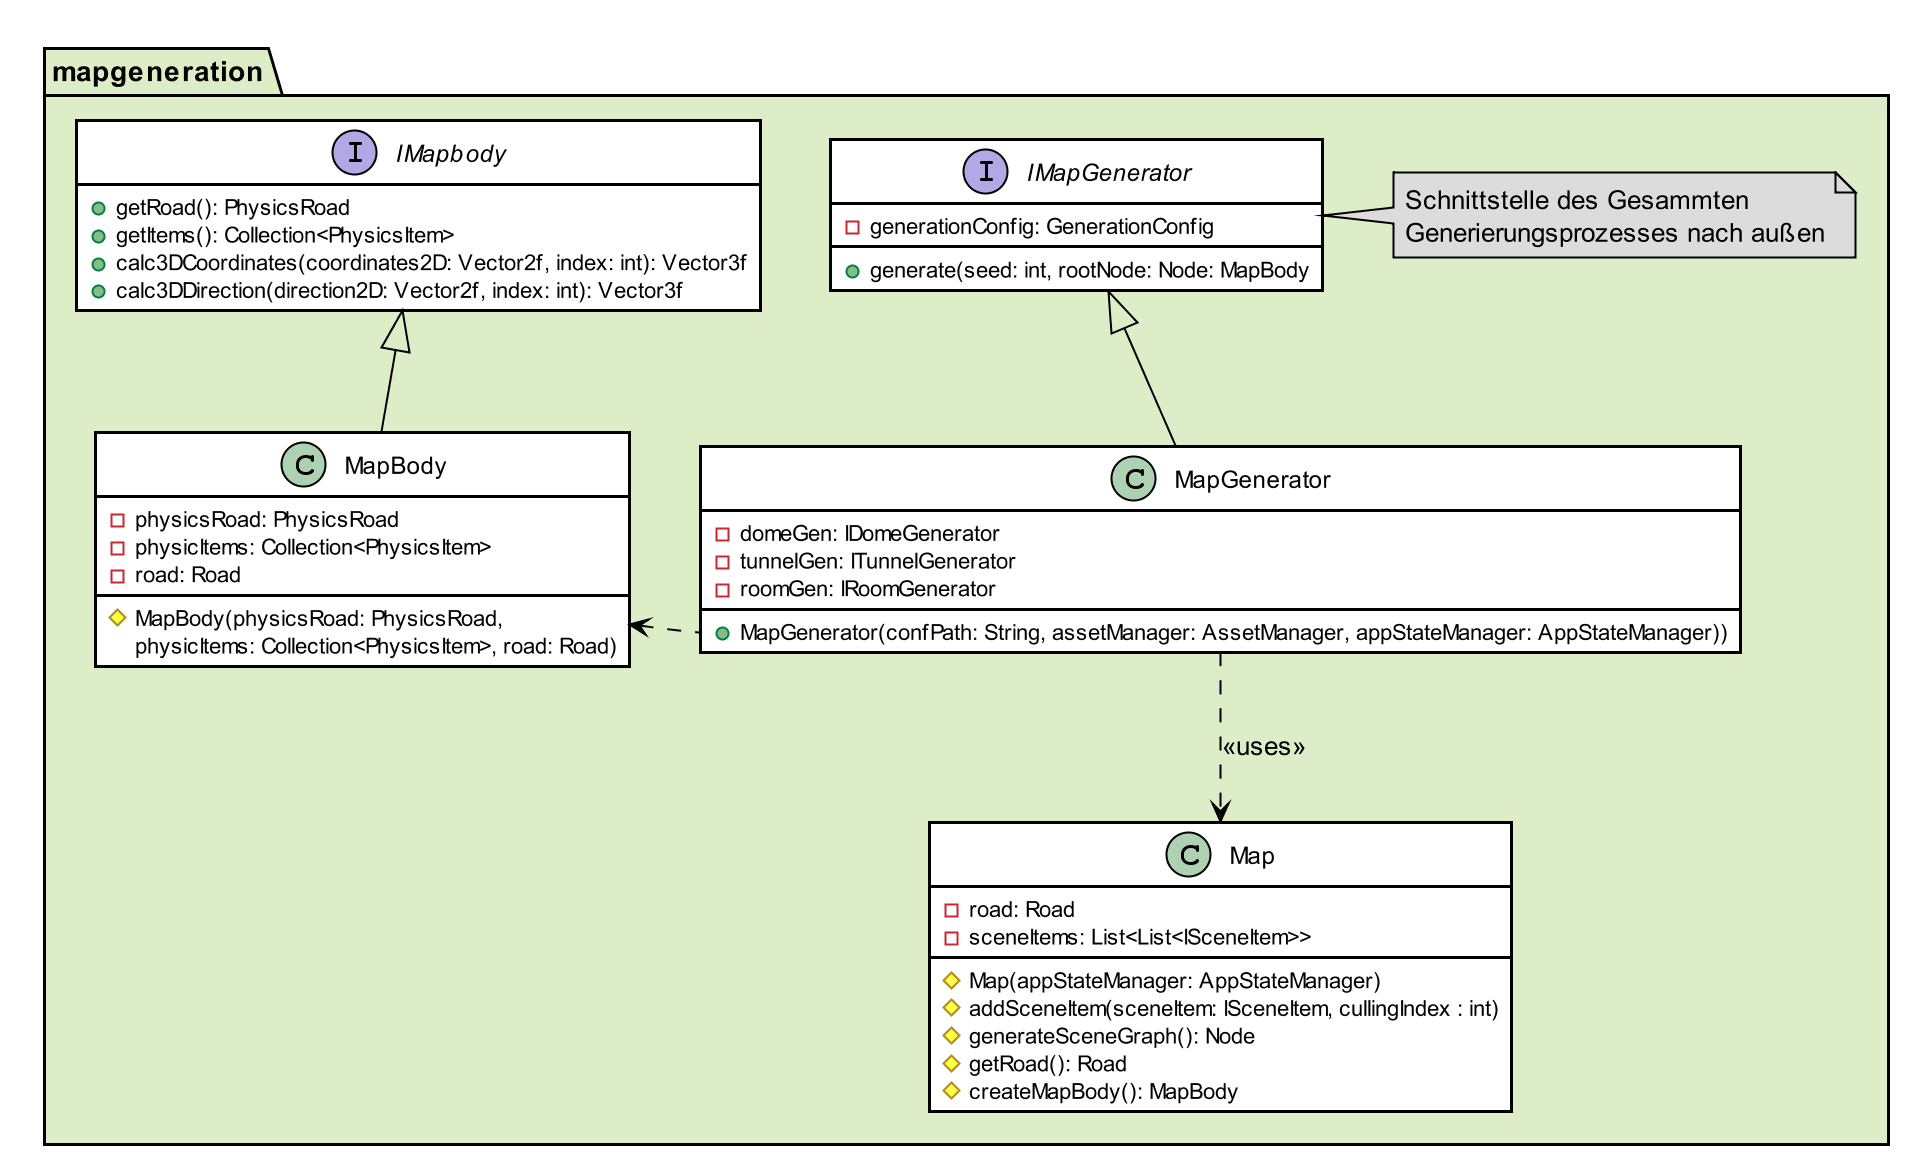
\includegraphics[width=\linewidth]{./Generierung/Bilder/mapgeneration.png}
        \caption{Klassendiagramm mapgeneration}
    \end{figure}


    \paragraph{\underline{IMapGenerator}} \mbox{}\par
            Schnittstelle, welche angesprochen werden kann um die prozedurale Generierung eine Karte, abhängig von 
            einem Seed, zu starten.\par
            
            \textbf{Methoden}					
            \begin{itemize}
                \item  \textit{+ generate(int seed, Node rootNode): MapBody}
                    \begin{leftbar}[0.9\linewidth]
                        Methode, welche die Generierung einer Karte, abhängig vom \textit{seed} einleitet
                         und dadurch einen \textit{IMapBody} zu erzeugen.\\
                        \textbf{@param seed} Zum generieren von Pseudozufallswerten.\\
                        \textbf{@param rootNode} Verwendet wie in \textit{JMonkey}, hier sollen alle Elemente der Karte 
                        angehängt werden.\\
                        \textbf{@return} Objekt einer Datenstruktur, dass die gesammte Strecke der Karte repräsentiert.
                    \end{leftbar} 
            \end{itemize}
    
    
    
        \paragraph{\underline{MapGenerator}} \mbox{}\par
            Implementiert \textit{IMapGenerator} und legt somit eine konkrete Implementierung für die Generierung fest.\par
            
            \textbf{Attribute}
            \begin{itemize}
                \item  \textit{- GenerationConfig generationConfig} 
                    \begin{leftbar}[0.9\linewidth]
                        Datenstruktur, die Parameter für die Generierung hält.
                    \end{leftbar}
                \item  \textit{- IDomeGenerator domeGen} 
                    \begin{leftbar}[0.9\linewidth]
                        Generator, der sich um die Generirung von Kuppeln kümmert.
                    \end{leftbar}
                \item  \textit{- ITunnelGenerator tunnelGen} 
                    \begin{leftbar}[0.9\linewidth]
                        Generator, der sich um die Generirung von Tunneln kümmert.
                    \end{leftbar}
                \item  \textit{- IRoomGenerator rommGen} 
                    \begin{leftbar}[0.9\linewidth]
                        Generator, der sich um die Generirung von Räumen kümmert.
                    \end{leftbar}
            \end{itemize}

            \textbf{Methoden}					
            \begin{itemize}
                \item  \textit{+ MapGenerator(String confPath, AssetManager assetManager)}
                    \begin{leftbar}[0.9\linewidth]
                        Konsrtuktor für \textit{MapGenerator}.\\
                        \textbf{@param confPath} Pfad zum JSON - Dokument, welches Parameter für die Generierung bereit hält.\\
                        \textbf{@param assetManager} Von \textit{JMonkey} vordefinierte Klasse, zum verwalten von Assets.
                    \end{leftbar}  
            \end{itemize}
    
    
    
        \paragraph{\underline{Map}} \mbox{}\par
            Datenstruktur, die die Karte während des Generierungsprozess repräsentiert. Enthält außerdem Funktionalität um einen 
            \textit{IMapBody} zu erzeugen.\par
            
            \textbf{Attribute}
            \begin{itemize}
                \item  \textit{- Road road} 
                    \begin{leftbar}[0.9\linewidth]
                        Repräsentiert die Straße, die durch die Karte verläuft.
                    \end{leftbar}
                
                \item  \textit{- List<List<ISceneItem>> sceneItems} 
                    \begin{leftbar}[0.9\linewidth]
                        Liste an \textit{sceneItems}, welche jeweils einen \textit{cullingIndex} besitzen.
                    \end{leftbar}
            \end{itemize}

            \pagebreak
            \textbf{Methoden}					
            \begin{itemize}
                \item  \textit{\# Map(appStateManager: AppStateManager)}
                    \begin{leftbar}[0.9\linewidth]
                        Konsrtuktor für \textit{Map}.\\
                        \textbf{@param appStateManager} Von \textit{JMonkey}übernommen, zum verwalten der \textit{Appstates}.
                    \end{leftbar}

                \item  \textit{\# addSceneItem(ISceneItem sceneItem, int cullingIndex)}
                    \begin{leftbar}[0.9\linewidth]
                        Fügt ein \textit{ISceneItem} zur Karte hinzu und erweitert diese so.\\
                        \textbf{@param sceneItem} Datenstruktur die einen Abschnitt der Karte, wie beispielsweise eine Kuppel, 
                        repräsentiert.
                        \textbf{@param cullingIndex} Nummerierung der Teilabschnitte einer Karte.
                    \end{leftbar}    
        
                \item  \textit{\# generateSceneGraph(): Node}
                    \begin{leftbar}[0.9\linewidth]
                        Gibt den SceneGraph, wie in \textit{JMonkex} verwendet, für die Karte zurück.\\
                        \textbf{@return} Verwendet wie in \textit{JMonkey}, wird übergeben um die Karte in einer Szene darzustellen.
                    \end{leftbar}    
            
                \item  \textit{\# getRoad(): Road}
                    \begin{leftbar}[0.9\linewidth]
                        \textbf{@return} Datenstruktur, die den Streckenverlauf der Karte beschreibt.
                    \end{leftbar}    
                
                \item  \textit{\# createMapBody(): MapBody}
                    \begin{leftbar}[0.9\linewidth]
                        \textbf{@return} Objekt einer Datenstruktur, dass die gesammte Strecke der Karte repräsentiert.
                    \end{leftbar}    
            \end{itemize}
    
    
    
         \paragraph{\underline{IMapBody}} \mbox{}\par
         Datenstruktur, die einen Streckenverlauf einer Karte repräsentiert. Hieru werden auch alle Objekte, die auf dieser 
         platziert sind gehalten.\par
            
            \textbf{Methoden}					
            \begin{itemize}
                \item  \textit{+ getRoad(): PhysicsRoad}
                \begin{leftbar}[0.9\linewidth]
                        \textbf{@return} Datenstruktur einer Strecke, die durch das andere Team definiert wird.
                    \end{leftbar}
                    
                    \item  \textit{+ getItems(): Collection<PhysicsItem>}
                    \begin{leftbar}[0.9\linewidth]
                        \textbf{@return} Datenstruktur, die Objekte auf der Strecke darstellt, definiert durch das andere Team.
                    \end{leftbar}    
                    
                    \item  \textit{+ calc3DCoordinates(Vector2f coordinates2D, int index): Vector3f}
                    \begin{leftbar}[0.9\linewidth]
                        Berechnet die 3D - Weltkoordinaten aus dem 2D - System des anderen Teams.\\
                        \textbf{@param coordinates2D} 2D - Koordinate aus dem System des anderen Teams.\\
                        \textbf{@param index} Indiziert einen \textit{RaodCursor} im Streckenverlauf.\\
                        \textbf{@return} 3D - Koordinate des Darstellungstyps \textit{Map} der Karte.
                    \end{leftbar}
                    
                    \item  \textit{+ calc3DDirection(Vector2f direction2D, int index): Vector3f}
                    \begin{leftbar}[0.9\linewidth]
                        Berechnet eine 3D - Vektor, der eine Richtung angibt, aus dem 2D - System des anderen Teams.\\
                        \textbf{@param direction2D} 2D - Vektor aus dem System des anderen Teams.\\
                        \textbf{@param index} Indiziert einen \textit{RaodCursor} im Streckenverlauf.\\
                        \textbf{@return} 3D - Vektor für eine Richtung im Darstellungstyp \textit{Map} der Karte.
                    \end{leftbar}    
                \end{itemize}
                
                
                
            \paragraph{\underline{MapBody}} \mbox{}\par
                Implementiert \textit{IMapBody} und implementiert somit die konkreten Brechnungen für das System des anderen Teams.
                    
                \textbf{Attribute}
                \begin{itemize}
                    \item  \textit{- PhysicsRoad physicsRoad} 
                        \begin{leftbar}[0.9\linewidth]
                            Datenstruktur einer Strecke, die durch das andere Team definiert wird.
                        \end{leftbar}
                
                    \item  \textit{- Collection<PhysicsItem> physicItems} 
                        \begin{leftbar}[0.9\linewidth]
                            Datenstruktur, die Objekte auf der Strecke darstellt, definiert durch das andere Team.
                        \end{leftbar}
                    
                    \item  \textit{- Road road} 
                        \begin{leftbar}[0.9\linewidth]
                            Datenstruktur den Streckenverlauf der Karte repräsentiert.
                        \end{leftbar}
                \end{itemize}
    
                \textbf{Methoden}					
                \begin{itemize}
                    \item  \textit{\# MapBody(PhysicsRoad physicsRoad, Collection<PhysicsItem> physicItems, Road road)}
                        \begin{leftbar}[0.9\linewidth]
                            Konsrtuktor für \textit{MapBody}.\\
                            \textbf{@param physicsRoad} Datenstruktur einer Strecke, die durch das andere Team definiert wird.\\
                            \textbf{@param physicItems} Datenstruktur, die Objekte auf der Strecke darstellt, definiert durch das andere Team.\\
                            \textbf{@param road} Datenstruktur den Streckenverlauf der Karte repräsentiert.\\
                        \end{leftbar}  
                \end{itemize}

    \pagebreak
    \subsubsection{generation.domegeneration}
    Domegeneration ist dafür verantwortlich eine Kuppel (\textit{AbstractDome}) zu Generieren,
    dies geschieht mit Hilfe der Implementrierungen einer Rauschfunktion (\textit{AbstractNoiseGenerator})
    und einer Objekt Generierungsfunktion (\textit{AbstractDomeAssetGenerator}). \par
   
    \begin{figure}[htbp]
        \centering
        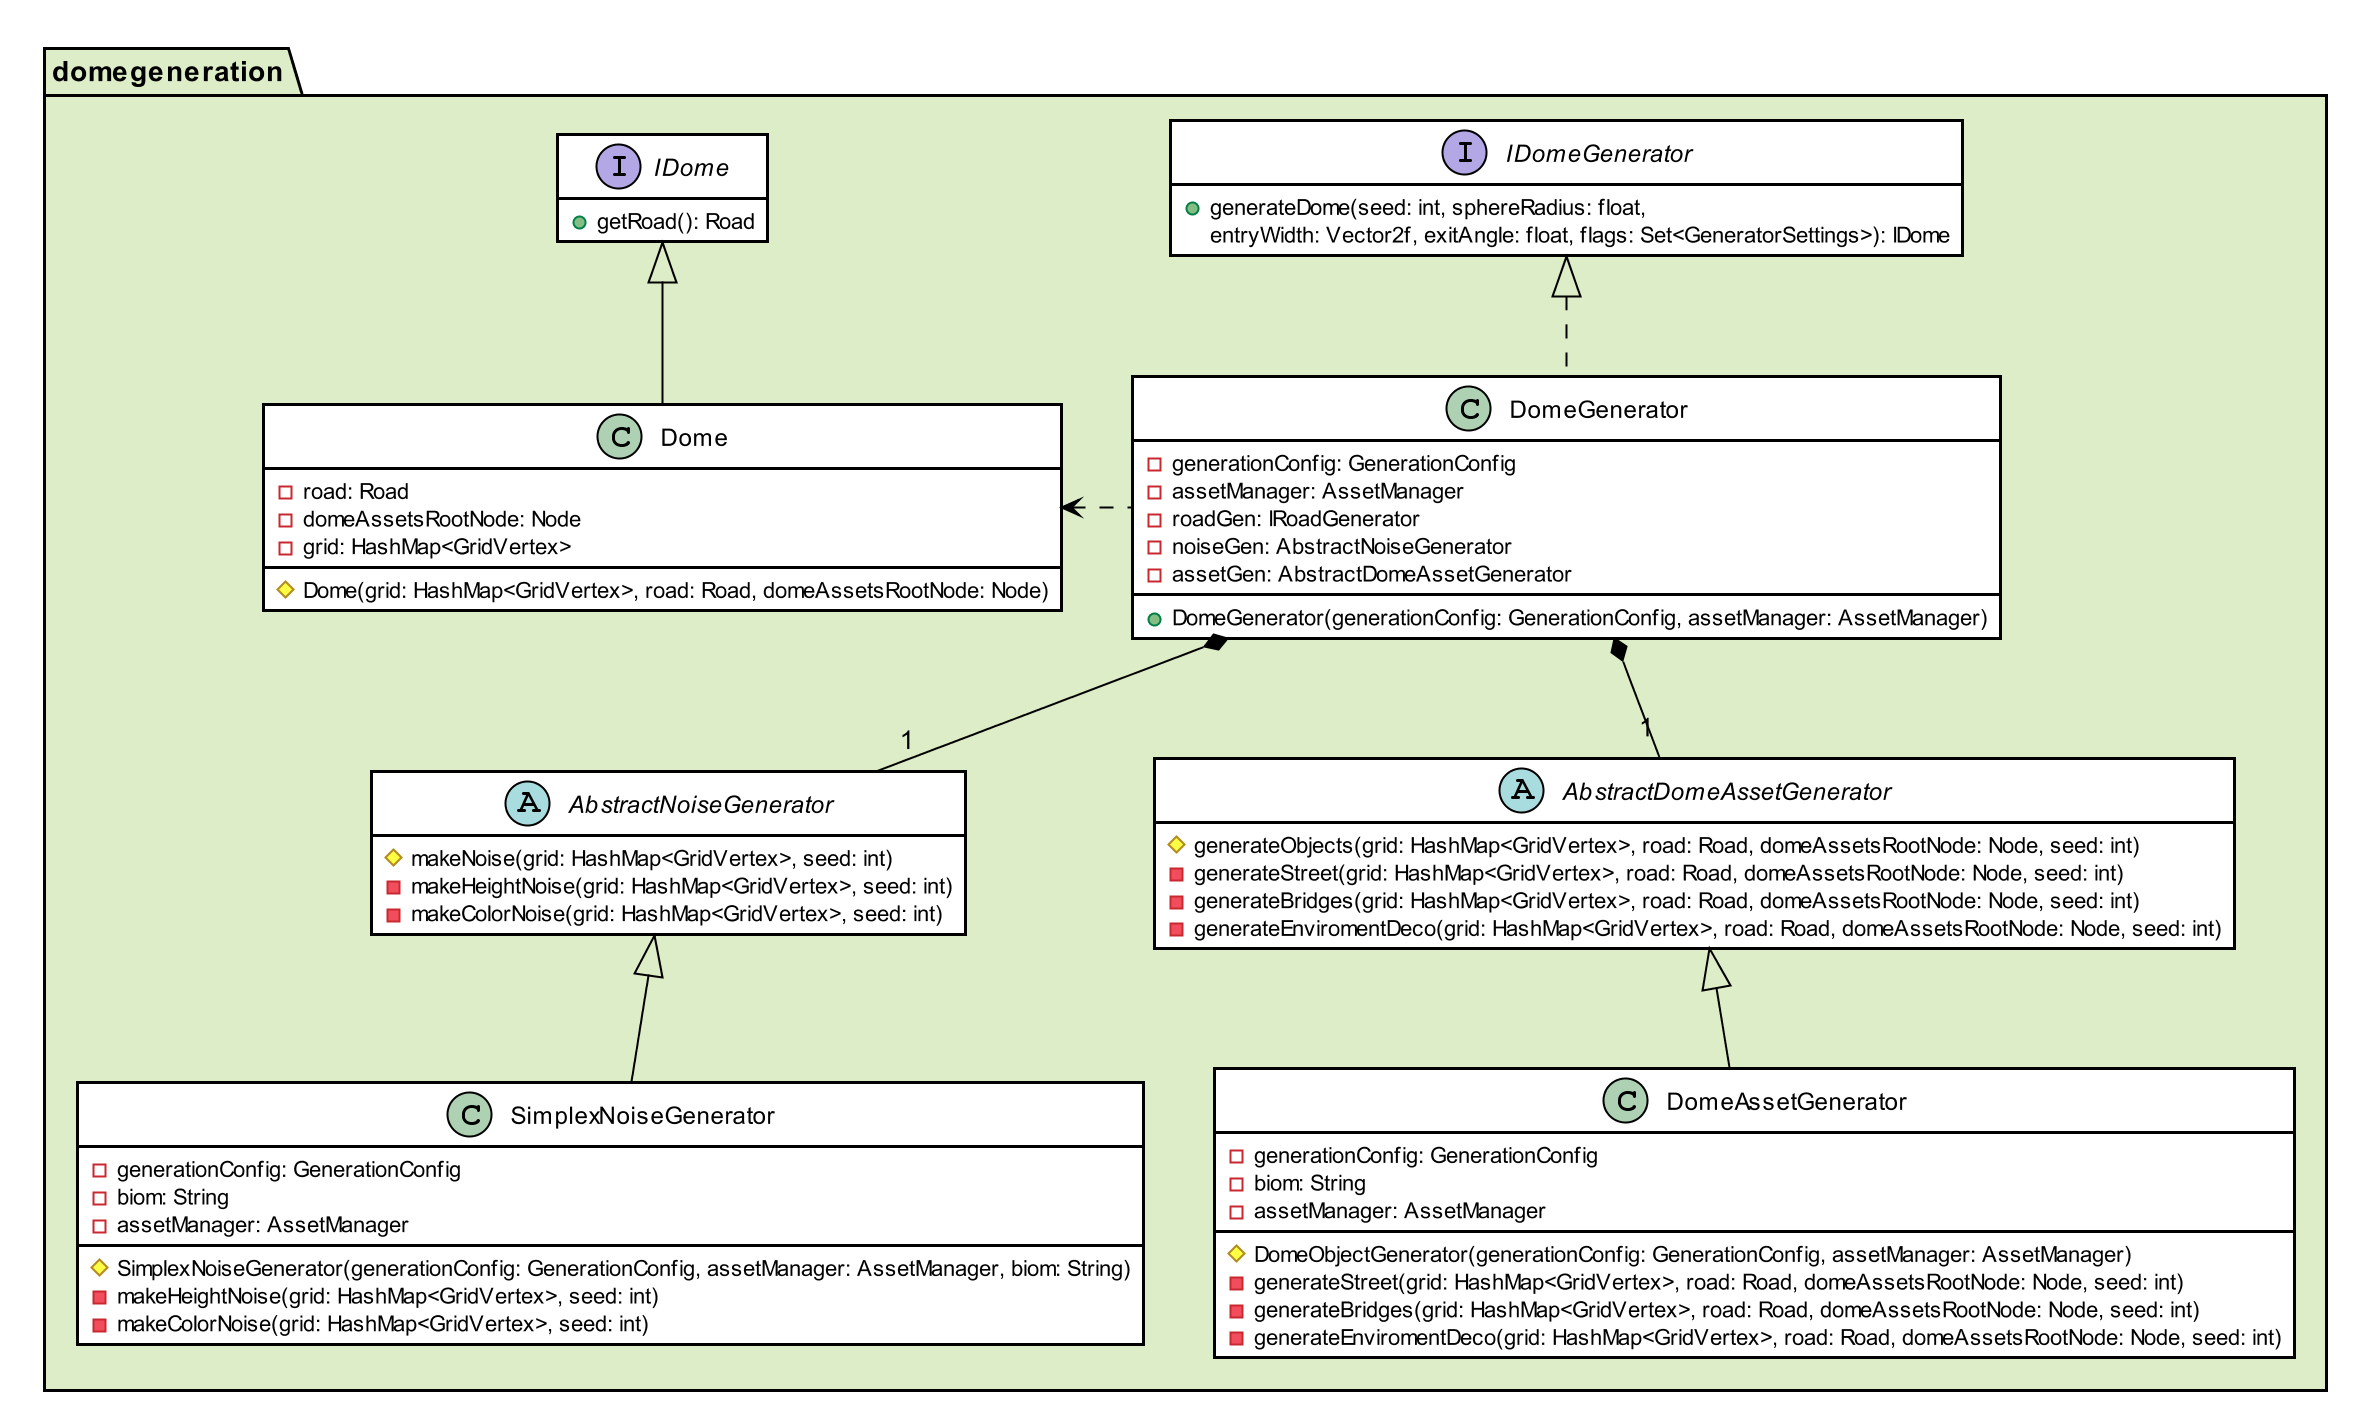
\includegraphics[width=\linewidth]{./Generierung/Bilder/domegeneration.png}
        \caption{Klassendiagramm domegeneration}
    \end{figure}


        \paragraph{\underline{IDomeGenerator}} \mbox{}\par
            Schnittstelle nach außsen, zur Genereirung einer Kupppel über welche sich der Genereirungsprozess
            anregen lässt. \textit{IDomeGenerator} bildet die abstrakte Fabrik im Entwurfmuster 'Fabrik'. \par
            
            \textbf{Methoden}					
            \begin{itemize}
                \item  \textit{+ generateDome(int seed, float sphereRadius,Vector2f entryWidth,
                                 float exitAngle, Set<GeneratorSettings> flags): IDome}
                    \begin{leftbar}[0.9\linewidth]
                        Stößt den Genereirungsprozess zu einem \textit{AbstractDome} an.\\
                        \textbf{@param seed} Zum generieren von Pseudozufallswerte.\\
                        \textbf{@param sphereRadius} Legt maximale Größe der Kuppel fest.\\
                        \textbf{@param entryWidth} Legt Dimensionen des Eingangs in die Kuppel fest.\\
                        \textbf{@param exitAngle} Legt Winkel zwischen Ein-/ und Ausgang fest, welcher angenähert
                            werden soll.\\
                        \textbf{@param flags} Menge an Präferenzen, die zur Generierung übergegben werden.\\
                        \textbf{@return} Datenstruktur, die eine Kuppel repräsentiert.
                    \end{leftbar}
            \end{itemize}


        \paragraph{\underline{DomeGenerator}} \mbox{}\par
            Konkrete Implementierung der Schnittstelle \textit{IDomeGenerator} und stellt somit die
            konkrete Fabrik im Entwurfsmuster 'Fabrik' dar welche einen konkreten \textit{Dome} generiert. \par
            
            \textbf{Attribute}
            \begin{itemize}
                \item  \textit{- GenerationConfig generationConfig} 
                    \begin{leftbar}[0.9\linewidth]
                        Datenstruktur, die Parameter für die Generierung hält.
                    \end{leftbar}
                
                \item  \textit{- AssetManager assetManager} 
                    \begin{leftbar}[0.9\linewidth]
                        Von \textit{JMonkey} vordefinierte Klasse, zum verwalten von Assets.
                    \end{leftbar}
            
                \item  \textit{- IRoadGenerator roadGen} 
                    \begin{leftbar}[0.9\linewidth]
                        Ist für die Generierung eines Streckenverlaufs verantwortlich.
                    \end{leftbar}
                
                \item  \textit{- AbstractNoiseGenerator noiseGen} 
                    \begin{leftbar}[0.9\linewidth]
                        Ist für die Generierung einer Rauschfunktion, um eine Landschaft zu erzeugen, zuständig.
                    \end{leftbar}
                
                \item  \textit{- AbstractDomeAssetGenerator assetGen} 
                    \begin{leftbar}[0.9\linewidth]
                        Verteilt verschiedenen Assets in der Landschaft, beispielsweise Dekoration.
                    \end{leftbar}
            \end{itemize}

            \textbf{Methoden}					
            \begin{itemize}
                \item  \textit{+ DomeGenerator(GenerationConfig generationConfig, AssetManager assetManager)}
                    \begin{leftbar}[0.9\linewidth]
                        Konsrtuktor von \textit{DomeGenerator}.\\
                        \textbf{@param generationConfig} Datenstruktur, die Parameter für die Generierung hält.\\
                        \textbf{@param assetManager} Von \textit{JMonkey} vordefinierte Klasse, zum verwalten von Assets.
                    \end{leftbar}
            \end{itemize}
            
            
            
            \paragraph{\underline{AbstractNoiseGenerator}} \mbox{}\par
            Definiert und implementiert die Grundvorraussetzungen für eine Rauschfuntion, 
            die eine an die Strecke angepasste Landschaft erzeugt.\par
            
            \textbf{Methoden}					
            \begin{itemize}
                \item  \textit{\# makeNoise(HashMap<GridVertex> grid, int seed)}
                    \begin{leftbar}[0.9\linewidth]
                        Generiert eine Rauschfunktion an Hand aller gegebenen Parameter, wie dem Biom, um eine Landschaft zu generieren,
                        die diesen entspricht.\\
                        \textbf{@param grid} Das Gitter der Kuppel, sodass ein Status eines \textit{GridVertex} abgerufen weren kann,
                            um die Rauschfunktion an Gegebenheiten wie Streckenhöhe anzupassen.\\
                        \textbf{@param seed} Zum generieren von Pseudozufallswerte.
                    \end{leftbar}  
            \end{itemize}



            

            \paragraph{\underline{SimplexNoisGenerator}} \mbox{}\par
            Erweitert \textit{AbstractNoiseGenerator} indem eine konkrete Rauschfunktion (\textit{SimplexNois}) implementiert wird.\par
            
            \textbf{Attribute}
            \begin{itemize}
                \item  \textit{- GenerationConfig generationConfig} 
                    \begin{leftbar}[0.9\linewidth]
                        Datenstruktur, die Parameter für die Generierung hält.
                    \end{leftbar}

                \item  \textit{- AssetManager assetManager} 
                    \begin{leftbar}[0.9\linewidth]
                        Von \textit{JMonkey} vordefinierte Klasse, zum verwalten von Assets.
                    \end{leftbar}
                
                \item  \textit{- String biom} 
                    \begin{leftbar}[0.9\linewidth]
                        Gibt an, wo im JSON - Dokument die Inforamtionen über das aktuelle Biom zu finden sind.
                    \end{leftbar}
            \end{itemize}


            \textbf{Methoden}					
            \begin{itemize}
                \item  \textit{\# SimplexNoisGenerator(GenerationConfig generationConfig,AssetManager assetManager, String biom)}
                    \begin{leftbar}[0.9\linewidth]
                        Konsrtuktor von \textit{SimplexNoisGenerator}.\\
                        \textbf{@param generationConfig} Datenstruktur, die Parameter für die Generierung hält.\\
                        \textbf{@param assetManager} Von \textit{JMonkey} vordefinierte Klasse, zum verwalten von Assets.\\
                        \textbf{@param biom} Gibt an, wo im JSON - Dokument die Inforamtionen über das aktuelle Biom stehen.
                    \end{leftbar}   
            \end{itemize}
            
            
            
            \paragraph{\underline{AbstractDomeAssetGenerator}} \mbox{}\par
            Definiert und implementiert die MindestAnforderungen eines AssetGenerators für eine Kuppel. Diese sind dafür zuständig Object, 
            die auf die Landschaft angepasst sind, zu erzeugen.\par

            \textbf{Methoden}					
            \begin{itemize}
                \item  \textit{\# generateObjects(HashMap<GridVertex> grid, Road road, Node domeAssetsRootNode, int seed)}
                    \begin{leftbar}[0.9\linewidth]
                        Erzeugt und verteilt Objekte an Hand der Eigenschaften der durch \textit{grid} mitgegebenen Landschaft. Dies wird schrittweise innerhalb
                            einer Schablonenmethode durchgeführt.\\
                        \textbf{@param grid} Repräsentiert eine Kuppel, indem für jedes Feld (\textit{GridVertex}) Eigenschaften gespeichert sind.\\
                        \textbf{@param road} Repräsentiert die Straße in einer Kuppel.\\
                        \textbf{@param domeAssetsRootNode} Node wie in JMonkey verwendet, hier werden alle Objekte für die Kuppel angehängt.\\
                        \textbf{@param seed} Zum generieren von Pseudozufallswerte.
                    \end{leftbar}  
            \end{itemize}
            
            
            
            \paragraph{\underline{DomeAssetGenerator}} \mbox{}\par
            Erweitert \textit{AbstractDomeAssetGenerator} in dem die Erzeugung von Objekten hier in einer konkreten Strategie Umgesetzt wird.\par
            
            \textbf{Attribute}
            \begin{itemize}
                \item  \textit{- GenerationConfig generationConfig} 
                    \begin{leftbar}[0.9\linewidth]
                        Datenstruktur, die Parameter für die Generierung hält.
                    \end{leftbar}

                    \item  \textit{- String biom} 
                    \begin{leftbar}[0.9\linewidth]
                        Gibt an, wo im JSON - Dokument die Inforamtionen über das aktuelle Biom zu finden sind.
                    \end{leftbar}
                
                \item  \textit{- AssetManager assetManager} 
                    \begin{leftbar}[0.9\linewidth]
                        Von \textit{JMonkey} vordefinierte Klasse, zum verwalten von Assets.
                    \end{leftbar}
            \end{itemize}

            \textbf{Methoden}					
            \begin{itemize}
                \item  \textit{\# DomeObjectGenerator(GenerationConfig generationConfig,String biom, AssetManager assetManager)}
                    \begin{leftbar}[0.9\linewidth]
                        Konsrtuktor für \textit{DomeObjectGenerator}.\\
                        \textbf{@param generationConfig} Datenstruktur, die Parameter für die Generierung hält.\\
                        \textbf{@param biom} Gibt an, wo im JSON - Dokument die Inforamtionen über das aktuelle Biom stehen.\\
                        \textbf{@param assetManager} Von \textit{JMonkey} vordefinierte Klasse, zum verwalten von Assets.
                    \end{leftbar}   
            \end{itemize}
            
            
            
            \paragraph{\underline{IDome}} \mbox{}\par
            Implementiert \textit{ISceneItem}. Definiert die Grundfunktionalität der Datenstruktur einer Kuppel.\par
            
            \textbf{Methoden}					
            \begin{itemize}
                \item  \textit{+ generateSceneGraph(): Node}
                    \begin{leftbar}[0.9\linewidth]
                        Berechnet Scenegraph der Kuppel und gibt ihn zurück.\\
                        \textbf{@return}  Verwendet wie in \textit{JMonkey}, wird übergeben um den Tunnel in einer Szene darzustellen.
                    \end{leftbar}

                \item  \textit{+ getRoad(): Road}
                    \begin{leftbar}[0.9\linewidth]
                        Gibt die Straße (\textit{Road}), die durch die Kuppel verläuft, zurück.\\
                        \textbf{@return} Repräsentiert die Straße in der Kuppel.
                    \end{leftbar}    
            \end{itemize}
            
            
            \pagebreak
            \paragraph{\underline{Dome}} \mbox{}\par
            Implementiert \textit{IDome} und bildet somit eine konkrete Datenstruktur, die eine Kuppel beschreibt.
            \textit{Dome} stellt das Konkrete Produkt im Entwurfmuster 'Fabrik'.\par
            
            \textbf{Attribute}
            \begin{itemize}
                \item  \textit{- HashMap<GridVertex> grid} 
                    \begin{leftbar}[0.9\linewidth]
                        Repräsentiert eine Kuppel, indem für jedes Feld (\textit{GridVertex}) Eigenschaften gespeichert sind.
                    \end{leftbar}

                \item  \textit{- Road road} 
                    \begin{leftbar}[0.9\linewidth]
                        Repräsentiert die Straße, die durch den \textit{Dome} verläuft.
                    \end{leftbar}
                
                \item  \textit{- Node domeAssetsRootNode} 
                    \begin{leftbar}[0.9\linewidth]
                        Wie in \textit{JMonkey} verwendet. Beinhaltet alle Objekten, die im \textit{Dome} verteilt sind.
                    \end{leftbar}
            \end{itemize}

            \textbf{Methoden}					
            \begin{itemize}
                \item  \textit{\# Dome(HashMap<GridVertex> gird, Road road, Node domeAssetsRootNode)}
                    \begin{leftbar}[0.9\linewidth]
                        Konsrtuktor für \textit{Dome}.\\
                        \textbf{@param grid} Ein Gitter, welches den Untergrund in der Kuppel repräsentiert. Ein \textit{GridVertex} speichert hierbei 
                            immer die Eigenschaften an einer Position.\\
                        \textbf{@param road} Repräsentiert die straße, die durch den \textit{Dome} verläuft.\\
                        \textbf{@param domeAssetsRootNode} Beinhaltet alle Objekten, die im \textit{Dome} verteilt sein werden.
                    \end{leftbar}    
            \end{itemize}
    \pagebreak
    \subsubsection{generation.tunnelgeneration}
    \textit{Tunnelgeneration} ist dafür verantwortlich einen Tunnel zu generieren, der andere Segmente einer Karte, 
    wie einen Ruam oder eine Kuppel, mit einander verbindet. Die Tunnel (\textit{ITunnel}) werden prozedural generiert 
    und sind von einem Seed abhängig.\par

    \begin{figure}[htbp]
        \centering
        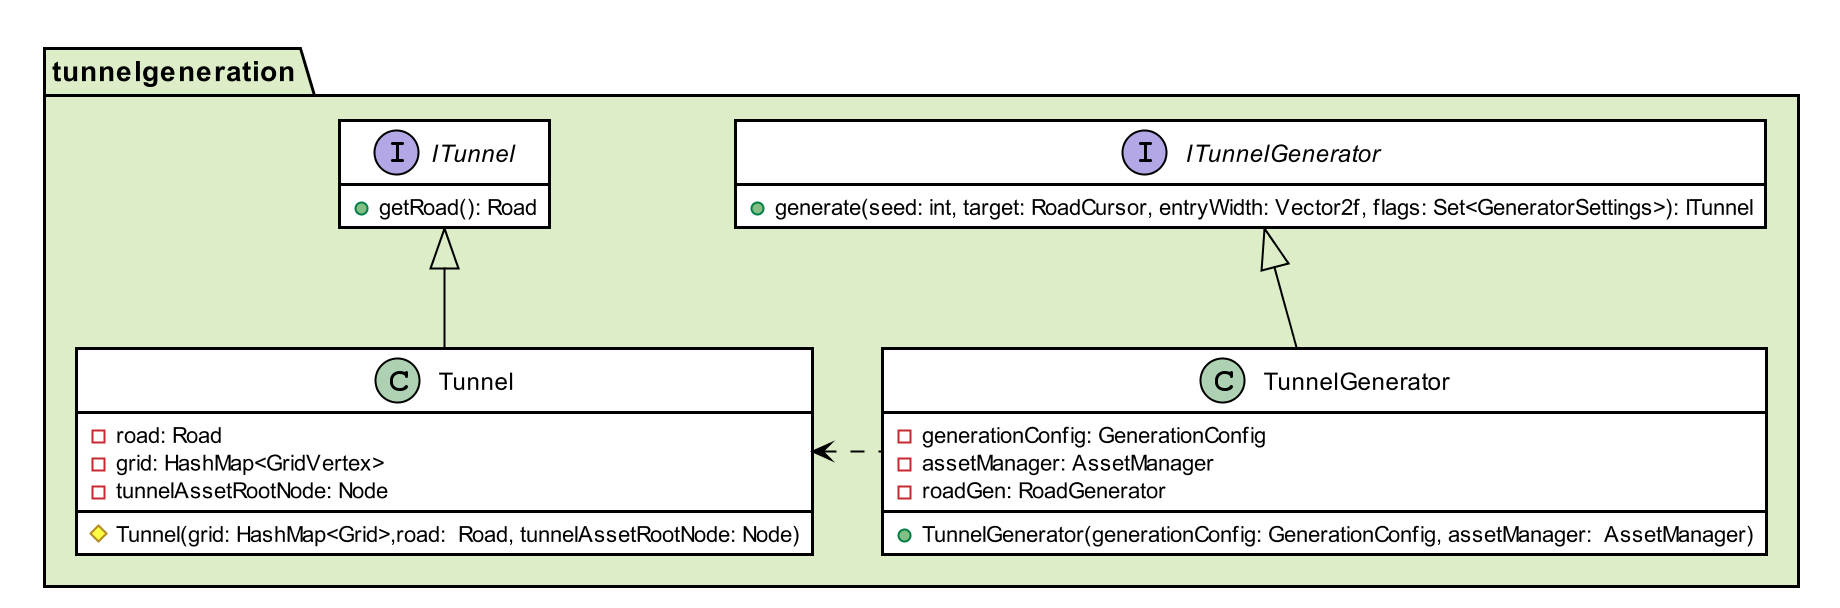
\includegraphics[width=\linewidth]{./Generierung/Bilder/tunnelgeneration.png}
        \caption{Klassendiagramm tunnelgeneration}
    \end{figure}


        \paragraph{\underline{ITunnelGenerator}} \mbox{}\par
            Schnittstelle um die Generierung eines Tunnels zwischen 2 Punkten anzuregen.\par
            
            \textbf{Methoden}					
            \begin{itemize}
                \item  \textit{+ generate(int seed, RoadCursor target, Vector2f entryWidth, Set<GeneratorSettings> flags): ITunnel}
                    \begin{leftbar}[0.9\linewidth]
                        Generiert einen Tunnel zwischen 2 Punkten, abhängig vom Seed und ggf. von flags.\\
                        \textbf{@param seed} Zum bestimmen von Pseuozufallswerten, die die Generierung bestimmen.\\
                        \textbf{@param target} Zielpunkt des zu generierenden Tunnels.\\
                        \textbf{@param entryWidth} Dimensionen für den Eingang des Tunnels.\\
                        \textbf{@param flags} Menge an Parametern, die als Präferenzen zur Generierung dienen.\\
                        \textbf{@return} Datenstruktur (\textit{ITunnel}), die einen Tunnel beschreibt.
                    \end{leftbar}   
            \end{itemize}
    
    
        \pagebreak
        \paragraph{\underline{TunnelGenerator}} \mbox{}\par
            Konkrete Imlementierung von \textit{ITunnelGenerator}, implementiert die Konkrete Generierungsfunktion für einen Tunnel
            zwischen 2 Punkten.\par
            
            \textbf{Attribute}
            \begin{itemize}
                \item  \textit{- GenerationConfig generationConfig} 
                    \begin{leftbar}[0.9\linewidth]
                        Datenstruktur, die Parameter für die Generierung hält.
                    \end{leftbar}
                
                \item  \textit{- AssetManager assetManager} 
                    \begin{leftbar}[0.9\linewidth]
                        Von \textit{JMonkey} vordefinierte Klasse, zum verwalten von Assets.
                    \end{leftbar}
                
                \item  \textit{- IRoadGenerator roadGen} 
                    \begin{leftbar}[0.9\linewidth]
                        Ist für die Generierung eines Streckenverlaufs verantwortlich.
                    \end{leftbar}
            \end{itemize}

            \textbf{Methoden}					
            \begin{itemize}
                \item  \textit{+ TunnelGenerator(GenerationConfig generationConfig, AssetManager assetManager)}
                    \begin{leftbar}[0.9\linewidth]
                        Konsrtuktor für \textit{TunnelGenerator}.\\
                        \textbf{@param generationConfig} Datenstruktur, die Parameter für die Generierung hält.\\
                        \textbf{@param assetManager}  Von \textit{JMonkey} vordefinierte Klasse, zum verwalten von Assets.
                    \end{leftbar} 
            \end{itemize}
    
    
       
        \paragraph{\underline{ITunnel}} \mbox{}\par
           Schnittstelle einer Datenstruktur, die einen Tunnel zwischen 2 Punkten beschreibt.\par

            \textbf{Methoden}					
            \begin{itemize}
                \item  \textit{+ generateSceneGraph(): Node}
                    \begin{leftbar}[0.9\linewidth]
                        Berechnet Scenegraph des Tunnelabschnitts und gibt ihn zurück.\\
                        \textbf{@return}  Verwendet wie in \textit{JMonkey}, wird übergeben um den Tunnel in einer Szene darzustellen.
                    \end{leftbar}

                \item  \textit{+ getRoad(): Road}
                    \begin{leftbar}[0.9\linewidth]
                        Gibt die Straße (\textit{Road}), die durch den Raum verläuft, zurück.\\
                        \textbf{@return} Repräsentiert die Straße in dem Raum.
                    \end{leftbar}     
            \end{itemize}
        
        
        \pagebreak
        \paragraph{\underline{Tunnel}} \mbox{}\par
            implementiert \textit{ITunnel}, stellt eine konkrete Datensturktur für einen Tunnel dar.\par
            
            \textbf{Attribute}
            \begin{itemize}
                \item  \textit{- Road road} 
                    \begin{leftbar}[0.9\linewidth]
                        Datenstruktur die eine Straße, die durch den Raum verläuft, repräsentiert.
                    \end{leftbar}
                
                \item  \textit{- HashMap<GridVertex> grid} 
                    \begin{leftbar}[0.9\linewidth]
                        Das Gitter des Tunnels, das verschiedene Stati pro \textit{GridVertex} speichert.
                    \end{leftbar}
                
                \item  \textit{- Node tunnelAssetRootNode} 
                    \begin{leftbar}[0.9\linewidth]
                        Verwendet wie in \textit{JMonkey}, hier soll der Tunnel angehängt werden.
                    \end{leftbar}
            \end{itemize}

            \textbf{Methoden}					
            \begin{itemize}
                \item  \textit{\# Tunnel(HashMap<Integer,GridVertex> grid, Road road, Node tunnelAssetRootNode)}
                    \begin{leftbar}[0.9\linewidth]
                        Konsrtuktor für \textit{Tunnel}.\\
                        \textbf{@param gird} Das Gitter des Tunnels, das verschiedene Stati pro \textit{GridVertex} speichert.\\
                        \textbf{@param road} Repräsentiert die Straße, die durch den Tunnel verläuft.\\
                        \textbf{@param tunnelAssetRootNode} Verwendet wie in \textit{JMonkey}, hier soll der Tunnel angehängt werden.
                    \end{leftbar}   
            \end{itemize}




    \pagebreak
    \subsubsection{generation.roomgeneration}
    \textit{Roomgeneration} ist dafür verantwortlich einen Raum zu generieren, der eine Straße besitzt und so 
    in eine Rennstrecke eingebaut werdenkann. Diser kann komplett prozedural generiert werden, aus einem Asset bestehen.
    Um das zu bewerkstelligen wird eine Liste von Generatoren (\textit{AbstractRoomGenerator}) verwaltet, welche
    auf unterschiedliche Weise Räume erstellen.\par

    \begin{figure}[htbp]
        \centering
        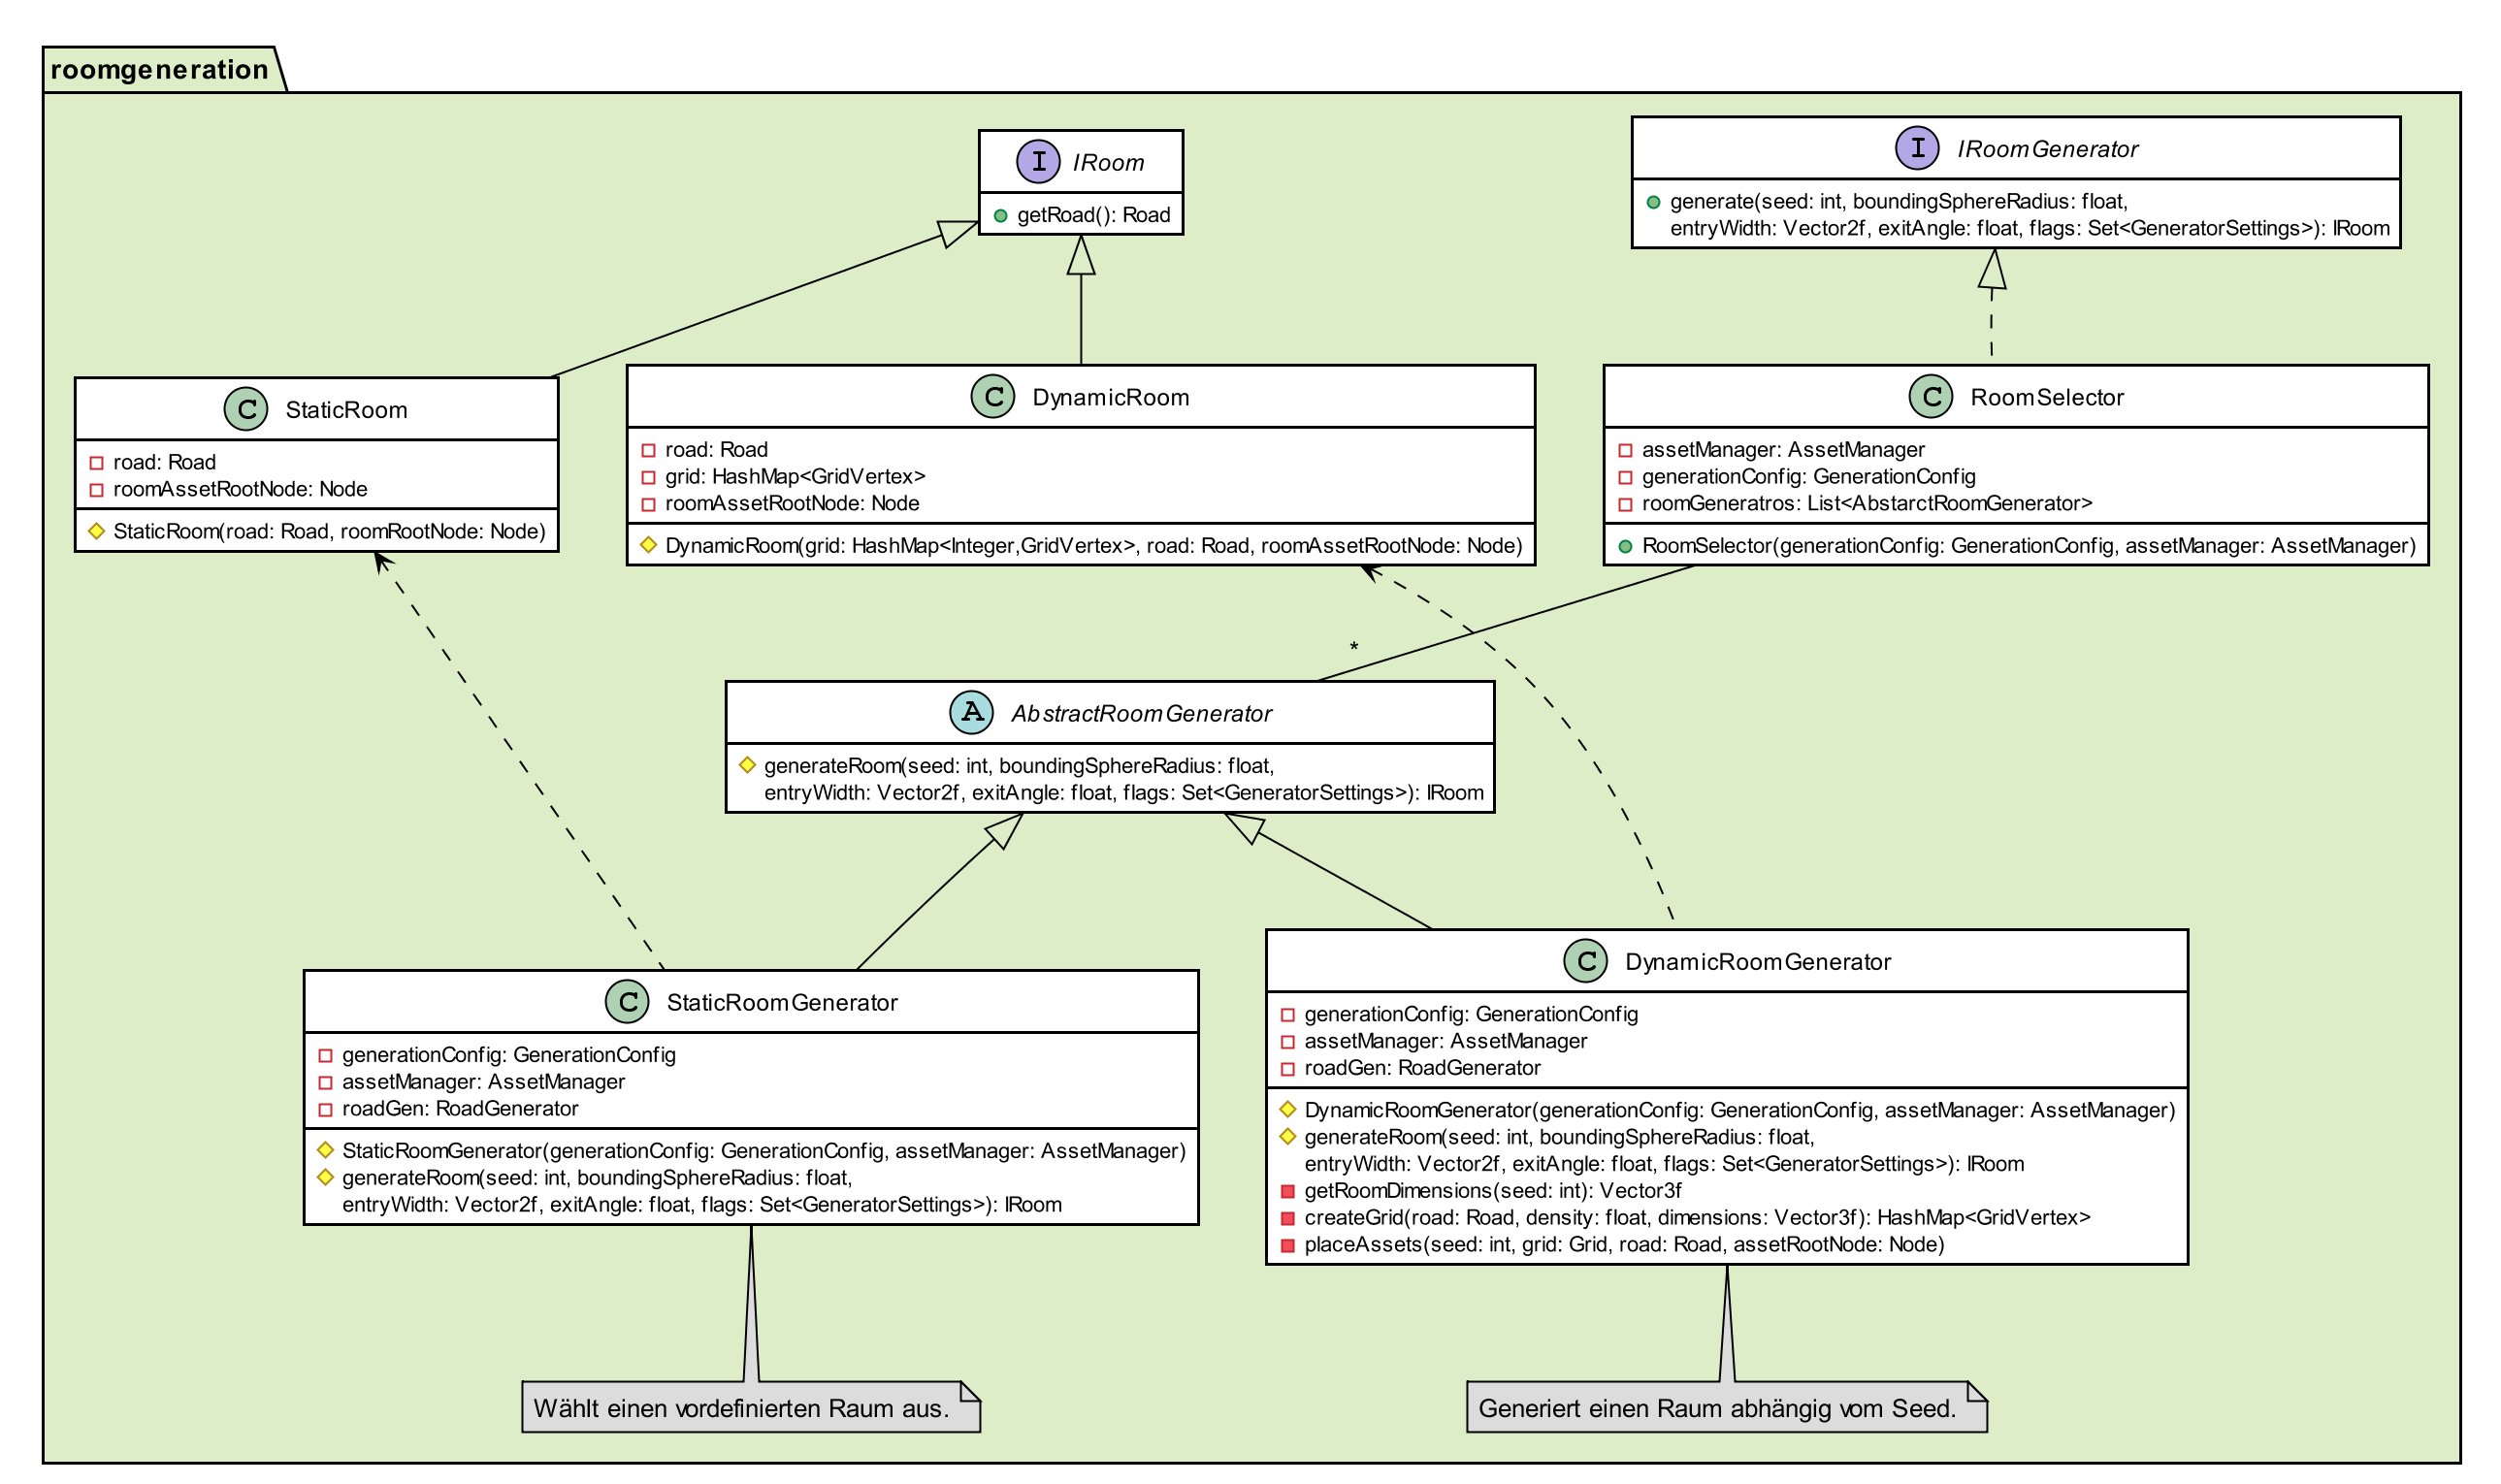
\includegraphics[width=\linewidth]{./Generierung/Bilder/roomgeneration.png}
        \caption{Klassendiagramm roomgeneration}
    \end{figure}

        \pagebreak
        \paragraph{\underline{IRoomGenerator}} \mbox{}\par
            Schnittstelle nach außen, um die Raumgenerieung anzustoßen, hierbei kann kein Einfluss auf die Art der Generierung 
            genommen werden.\par
            
            \textbf{Methoden}					
            \begin{itemize}
                \item  \textit{+ generate(int seed, float boundingSphereRadius,Vector2f entryWidth, float exitAngle, Set<GeneratorSettings> flags): IRoom}
                    \begin{leftbar}[0.9\linewidth]
                        Stößt den Generierungsprozess eines Raumes (\textit{IRoom}) an.\\
                        \textbf{@param seed} Zum bestimmen von Pseudozufallswerten.\\
                        \textbf{@param boundingSphereRadius} Definiert einen Kreis, indem der Raum bleiben muss, um seine Maße einzugrenzen.\\
                        \textbf{@param entryWidth} Bschreibt die Dimension des Eingangs.\\
                        \textbf{@param exitAngle} Bschreibt den Winkel zwischen Ein-/ und Ausgang.\\
                        \textbf{@param flags} Menge an Präferenzen, die zur Generierung übergegben werden.\\
                        \textbf{@return} Datenstruktur, die einen Raum repräsentiert.
                    \end{leftbar}   
            \end{itemize}
            
        
        
        \paragraph{\underline{RoomSelector}} \mbox{}\par
            Implementiert \textit{IRoomGenerator} führt jedoch keine echte Generierungan durch sondern hält ein Set von Generatoren (\textit{AbstractRoomGenerator}),
            von denen er jeweils einen auswählt, um durch diesen die Generierung ausführen zu lassen.\par
            
            \textbf{Attribute}
            \begin{itemize}
                \item  \textit{- AssetManager assetManager} 
                    \begin{leftbar}[0.9\linewidth]
                        Von \textit{JMonkey} vordefinierte Klasse, zum verwalten von Assets.
                    \end{leftbar}
                
                \item  \textit{- GenerationConfig generationConfig} 
                    \begin{leftbar}[0.9\linewidth]
                        Datenstruktur, die Parameter für die Generierung hält.
                    \end{leftbar}
                
                    \item  \textit{- List<AbstarctRoomGenerator> roomGeneratros} 
                    \begin{leftbar}[0.9\linewidth]
                        Datenstruktur, die Parameter für die Generierung hält.
                    \end{leftbar}
            \end{itemize}

            \textbf{Methoden}					
            \begin{itemize}
                \item  \textit{+ RoomSelector(GenerationConfig generationConfig, AssetManager assetManager)}
                    \begin{leftbar}[0.9\linewidth]
                        Konsrtuktor für \textit{RoomSelector}. Erstellt eine Menge an Generatoren des Typs \textit{AbstarctRoomGenerator} 
                        aus denen für die eigentliche Generierung jedes mal einer ausgewählt werden kann.\\
                        \textbf{@param generationConfig} Datenstruktur, die Parameter für die Generierung hält.\\
                        \textbf{@param assetManager} Von \textit{JMonkey} vordefinierte Klasse, zum verwalten von Assets.
                    \end{leftbar}   
            \end{itemize}
            
        
        
        \paragraph{\underline{AbstractRoomGenerator}} \mbox{}\par
            Definiert und implementiert die Grundfunktionalität, die jeder Generator eines \textit{IRoom} erfüllen muss.\par
            
            \textbf{Methoden}					
            \begin{itemize}
                \item  \textit{\# generateRoom(int seed, float boundingSphereRadius,Vector2f entryWidth, float exitAngle, Set<GeneratorSettings> flags): IRoom}
                    \begin{leftbar}[0.9\linewidth]
                        Stößt den Generierungsprozess eines Raumes (\textit{IRoom}) an.\\
                        \textbf{@param seed} Zum bestimmen von Pseudozufallswerten.\\
                        \textbf{@param boundingSphereRadius} Definiert einen Kreis, indem der Raum bleiben muss, um seine Maße einzugrenzen.\\
                        \textbf{@param entryWidth} Bschreibt die Dimension des Eingangs.\\
                        \textbf{@param exitAngle} Bschreibt den Winkel zwischen Ein-/ und Ausgang.\\
                        \textbf{@param flags} Menge an Präferenzen, die zur Generierung übergegben werden.\\
                        \textbf{@return} Datenstruktur, die einen Raum repräsentiert.
                    \end{leftbar}   
            \end{itemize}
        
        
        
        \paragraph{\underline{DynamicRoomGenerator}} \mbox{}\par
            Erweitert \textit{AbstractRoomGenerator} in durch eine konkrete Impementirung der \textit{generate()} Funktion.
            Hierbei wird ein Raum prozedural generiert, indem er aus verschiedenen Assets zusammen gesetzt wird.\par
            
            \textbf{Attribute}
            \begin{itemize}
                \item  \textit{- GenerationConfig generationConfig} 
                    \begin{leftbar}[0.9\linewidth]
                        Datenstruktur, die Parameter für die Generierung hält.
                    \end{leftbar}
                
                \item  \textit{- AssetManager assetManager} 
                    \begin{leftbar}[0.9\linewidth]
                        Von \textit{JMonkey} vordefinierte Klasse, zum verwalten von Assets.
                    \end{leftbar}
                
                \item  \textit{- IRoadGenerator roadGen} 
                    \begin{leftbar}[0.9\linewidth]
                        Ist für die Generierung eines Streckenverlaufs verantwortlich.
                    \end{leftbar}
            \end{itemize}

            \textbf{Methoden}					
            \begin{itemize}
                \item  \textit{\# DynamicRoomGenerator(GenerationConfig generationConfig, AssetManager assetManager)}
                    \begin{leftbar}[0.9\linewidth]
                        Konsrtuktor für \textit{DynamicRoomGenerator}.\\
                        \textbf{@param generationConfig} Datenstruktur, die Parameter für die Generierung hält.\\
                        \textbf{@param assetManager}  Von \textit{JMonkey} vordefinierte Klasse, zum verwalten von Assets.
                    \end{leftbar} 
            \end{itemize}
        
        
        \pagebreak
        \paragraph{\underline{StaticRoomGenerator}} \mbox{}\par
            Erweitert \textit{AbstractRoomGenerator} in durch eine konkrete Impementirung der \textit{generate()} Funktion.
            Hierbei wird jedoch lediglich ein Asset, das einen ganzen Raum repräsentiert, geladen.\par
                
            \textbf{Attribute}
            \begin{itemize}
                \item  \textit{- GenerationConfig generationConfig} 
                    \begin{leftbar}[0.9\linewidth]
                        Datenstruktur, die Parameter für die Generierung hält.
                    \end{leftbar}
                
                \item  \textit{- AssetManager assetManager} 
                    \begin{leftbar}[0.9\linewidth]
                        Von \textit{JMonkey} vordefinierte Klasse, zum verwalten von Assets.
                    \end{leftbar}
                
                \item  \textit{- IRoadGenerator roadGen} 
                    \begin{leftbar}[0.9\linewidth]
                        Ist für die Generierung eines Streckenverlaufs verantwortlich.
                    \end{leftbar}
            \end{itemize}

            \textbf{Methoden}					
            \begin{itemize}
                \item  \textit{\# StaticRoomGenerator(GenerationConfig generationConfig, AssetManager assetManager)}
                    \begin{leftbar}[0.9\linewidth]
                        Konsrtuktor für \textit{StaticRoomGenerator}.\\
                        \textbf{@param generationConfig} Datenstruktur, die Parameter für die Generierung hält.\\
                        \textbf{@param assetManager}  Von \textit{JMonkey} vordefinierte Klasse, zum verwalten von Assets.
                    \end{leftbar}  
            \end{itemize}
        
        
        
        \paragraph{\underline{IRoom}} \mbox{}\par
            Definiert die Grundfunktionalität der Datenstruktur eines Raums.\par

            \textbf{Methoden}					
            \begin{itemize}
                \item  \textit{+ generateSceneGraph(): Node}
                    \begin{leftbar}[0.9\linewidth]
                        Berechnet Scenegraph des Raums und gibt ihn zurück.\\
                        \textbf{@return}  Verwendet wie in \textit{JMonkey}, wird übergeben um den Tunnel in einer Szene darzustellen.
                    \end{leftbar}

                \item  \textit{+ getRoad(): Road}
                    \begin{leftbar}[0.9\linewidth]
                        Gibt die Straße (\textit{Road}), die durch den Raum verläuft, zurück.\\
                        \textbf{@return} Repräsentiert die Straße in dem Raum.
                    \end{leftbar}    
            \end{itemize}
        
        
        \pagebreak
        \paragraph{\underline{DynamicRoom}} \mbox{}\par
            Impementiert \textit{IRoom} und bildet somit eine konkrete Datenstruktur, die einen Raum, der prozedural generiert wurde, beschreibt.\par
            
            \textbf{Attribute}
            \begin{itemize}
                \item  \textit{- Road road} 
                    \begin{leftbar}[0.9\linewidth]
                        Datenstruktur die eine Straße, die durch den Raum verläuft, repräsentiert.
                    \end{leftbar}
                
                \item  \textit{- HashMap<GridVertex> grid} 
                    \begin{leftbar}[0.9\linewidth]
                        Das Gitter des Raumes, das verschiedene Stati pro \textit{GridVertex} speichert.
                    \end{leftbar}
                
                \item  \textit{- Node roomAssetRootNode} 
                    \begin{leftbar}[0.9\linewidth]
                        Verwendet wie in \textit{JMonkey}, hier sollen alle Objekte aus dem Raum angehängt werden.
                    \end{leftbar}
            \end{itemize}

            \textbf{Methoden}					
            \begin{itemize}
                \item  \textit{\# DynamicRoom(HashMap<Integer,GridVertex> grid, Road road, Node roomAssetRootNode)}
                    \begin{leftbar}[0.9\linewidth]
                        Konsrtuktor für \textit{DynamicRoom}.\\
                        \textbf{@param gird} Das Gitter des Raumes, das verschiedene Stati pro \textit{GridVertex} speichert.\\
                        \textbf{@param road} Repräsentiert die Straße, die durch den Raum verläuft.\\
                        \textbf{@param roomAssetRootNode} Verwendet wie in \textit{JMonkey}, hier sollen alle Objekte aus dem Raum angehängt werden.
                    \end{leftbar}   
            \end{itemize}
        
        
        \pagebreak
        \paragraph{\underline{StaticRoom}} \mbox{}\par
         Impementiert \textit{IRoom} und bildet somit eine konkrete Datenstruktur, die einen Raum, der aus einem Asset besteht, beschreibt.\par
            
            \textbf{Attribute}
            \begin{itemize}
                \item  \textit{- Road road} 
                    \begin{leftbar}[0.9\linewidth]
                        Datenstruktur, die die Straße, die durch den Raum verläuft repräsentiert.
                    \end{leftbar}
                
                \item  \textit{- Node roomRootNode} 
                    \begin{leftbar}[0.9\linewidth]
                        Verwendet wie in \textit{JMonkey}, hier sollen der Raum angehängt werden.
                    \end{leftbar}
            \end{itemize}

            \textbf{Methoden}					
            \begin{itemize}
                \item  \textit{\# StaticRoom(Road road, Node roomRootNode)}
                    \begin{leftbar}[0.9\linewidth]
                        Konsrtuktor für \textit{StaticRoom}.\\
                        \textbf{@param road} Repräsentiert die STraße, die durch den Raum verläuft.\\
                        \textbf{@param roomRootNode}  Verwendet wie in \textit{JMonkey}, hier sollen der Raum angehängt werden.
                    \end{leftbar}
 
            \end{itemize}

       
       
       
        
        
        
        
    \pagebreak
    \subsubsection{generation.roadgeneration}
    \textit{Roadgeneration} kapselt die Logik zur Generierung des eigentlichen Streckenverlaufs (\textit{Road}).\\
    Es bietet den anderen Generatoren Methoden zur Generierung unterschiedlicher Streckensegmente.\par

    \begin{figure}[htbp]
        \centering
        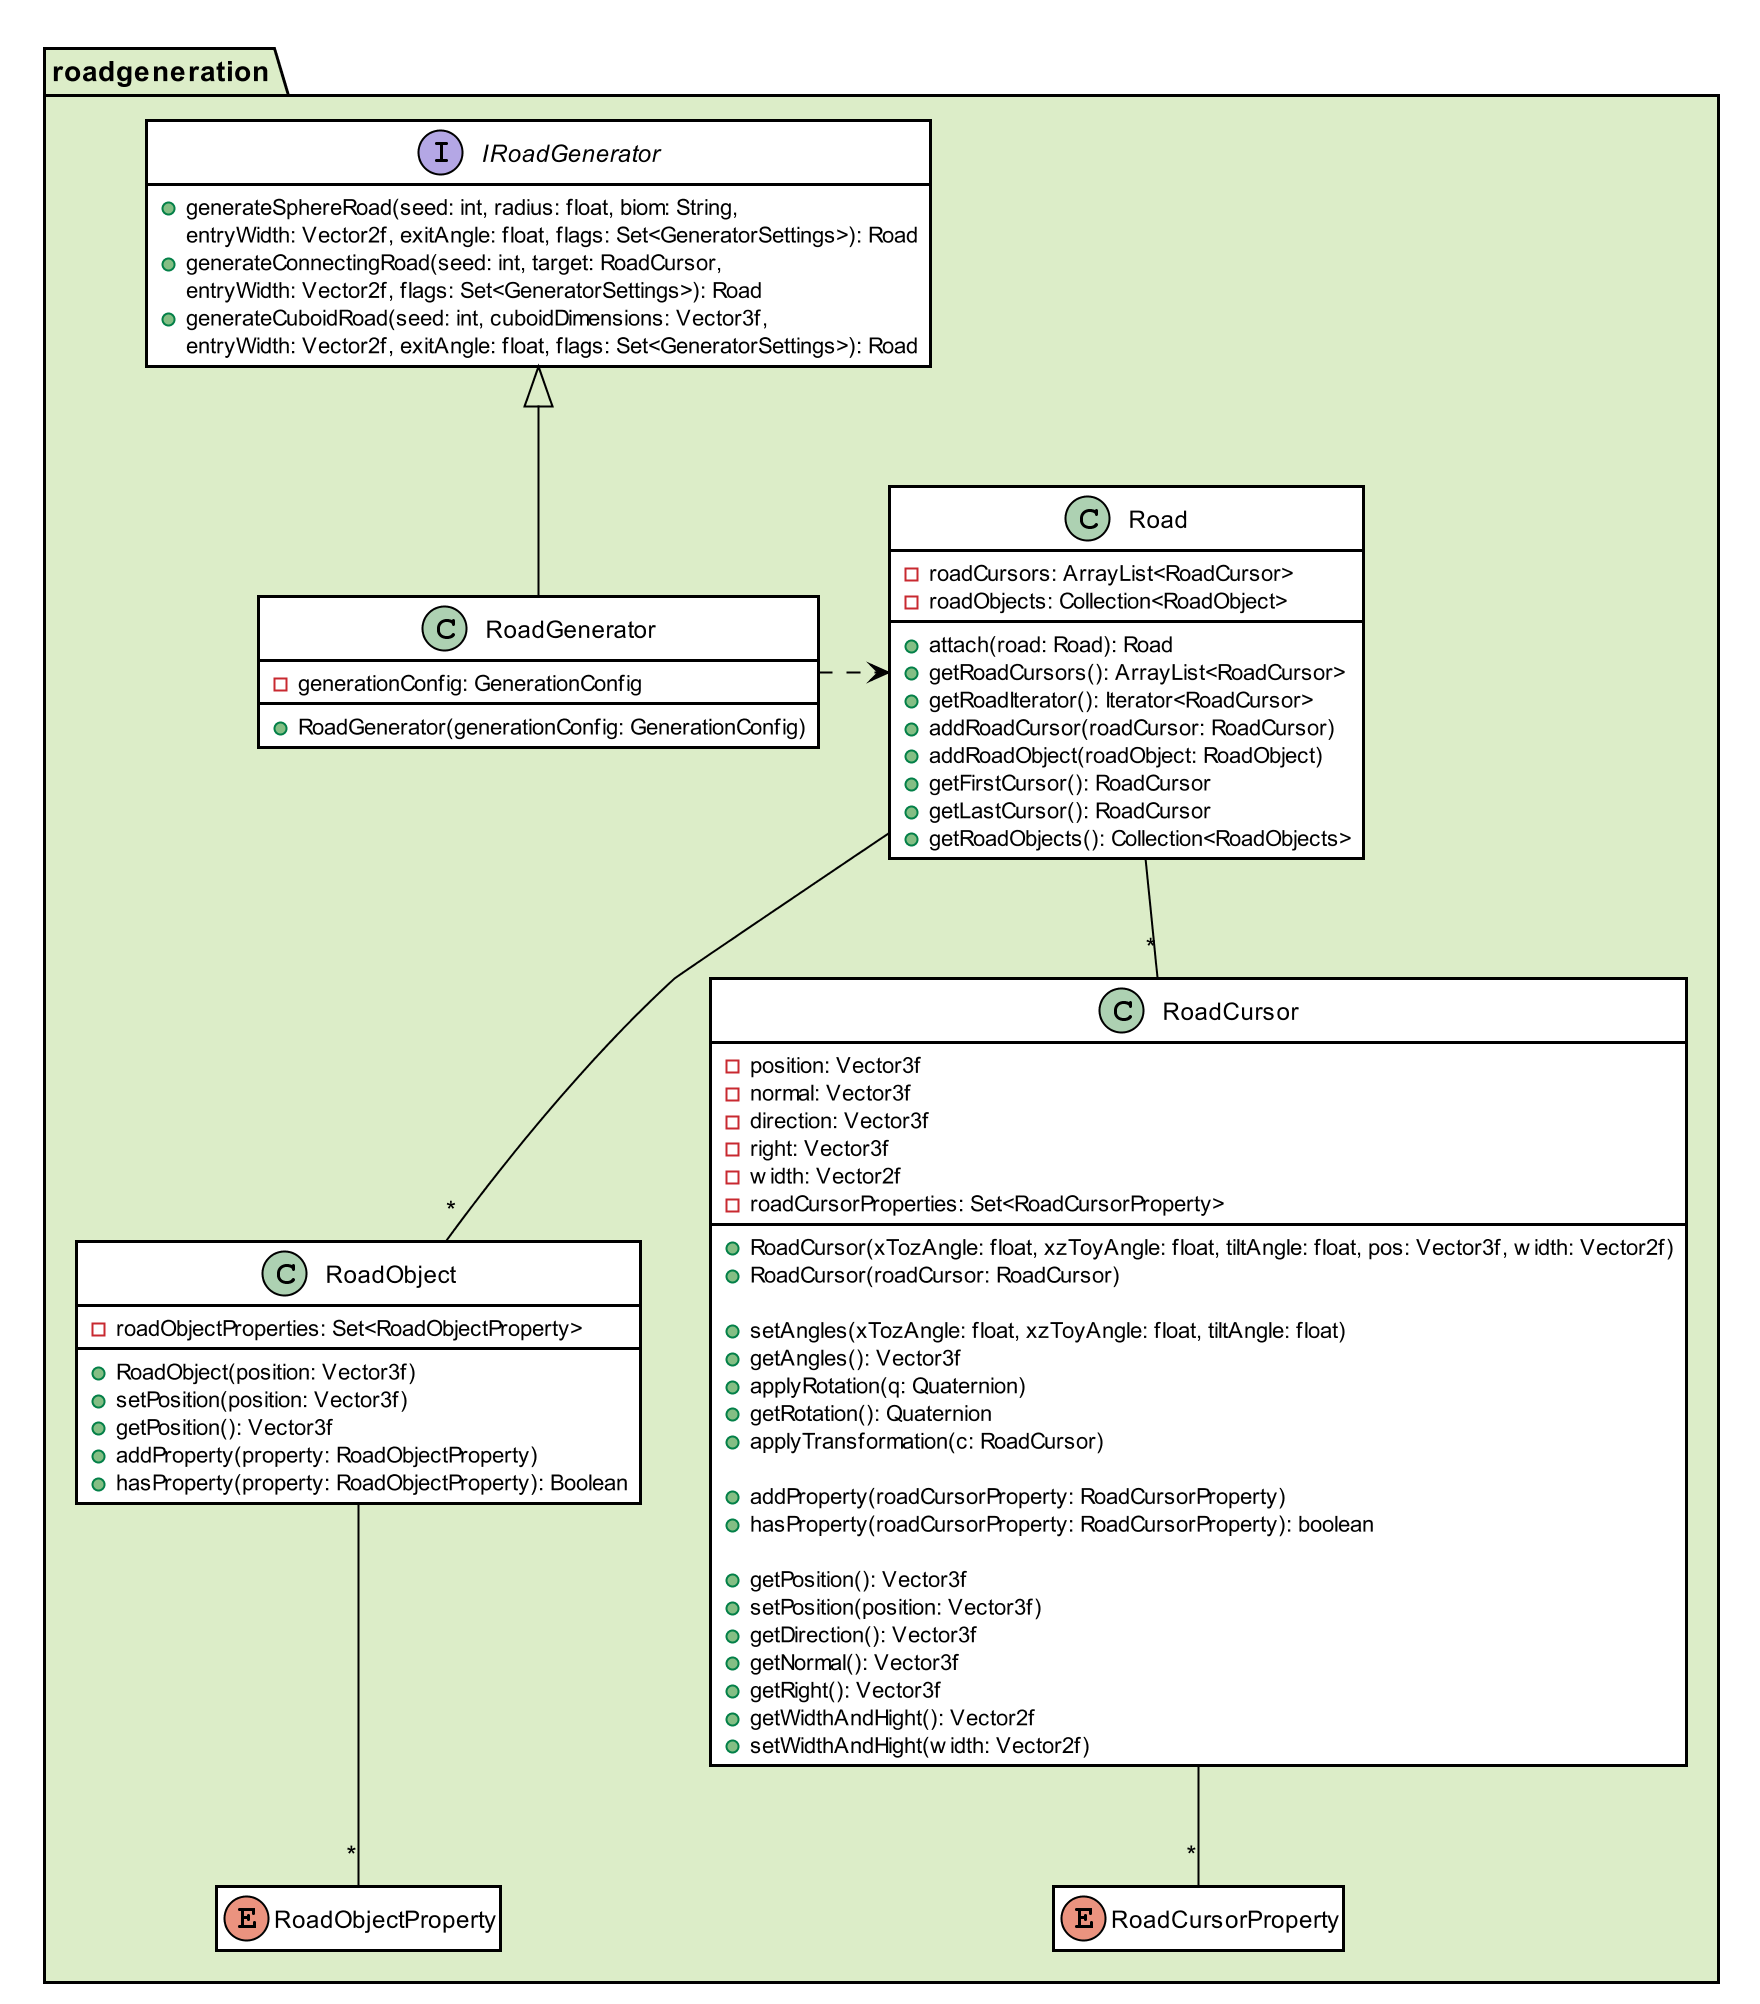
\includegraphics[width=0.9\linewidth]{./Generierung/Bilder/roadgeneration.png}
        \caption{Klassendiagramm domegeneration}
    \end{figure}

        \pagebreak
        \paragraph{\underline{IRoadGenerator}} \mbox{}\par
            Schnittstelle zur Generierung eines Streckenabschnitts.
            Ein ausgegebener Streckenabschnitt begint immer am Startpunkt (0,0,0) und Verläuft am Start in Z-Richtung.
            \par
            
            \textbf{Methoden}
            \begin{itemize}
                \item  \textit{+ generateSphereRoad(int seed, float radius, String biom,
                Vector2f entryWidth, float exitAngle, Collection<GeneratorSettings> flags): Road}
                    \begin{leftbar}[0.9\linewidth]
                        Erzeugt eine Strecke in einer Halbkugel, gegeben durch den Radius (\textit{radius}).\\
                        Die Strecke beginnt am Rande der Halbkugel.\\
                        Danach nimmt sie einen scheinbar belibigen Verlauf innerhalb der Halbkugel an.
                        Die Ausprägung des Verlaufs hängt vom Biom (\textit{biom}) ab.\\
                        Die Strecke terminiert wieder am Rande der Halbkugel.\\
                        Die Strecke kollidiert nie mit sich selber.\\
                        \textbf{@param seed} Zum bestimmen von Pseuozufallswerten, die den Verlauf der Strecke bestimmen.\\
                        \textbf{@param radius} Radius der Halbkugel.\\
                        \textbf{@param biom} Bestimmt Ausprägung der Stecke.\\
                        \textbf{@param entryWidth} Bestimmt den Querschnitt der Strecke am Eingang.\\
                        \textbf{@param exitAngle} Zahl zwischen [-Pi,PI]. Präferierter Winkel zwischen Ein- und Ausgang.\\
                        \textbf{@param Collection<GeneratorSettings> flags} Kollektion an Parametern, die als Präferenzen zur Generierung dienen.\\
                        \textbf{@return} Datenstruktur (\textit{Road}), die eine Strecke beschreibt.
                    \end{leftbar}

                \item  \textit{+ generateConnectingRoad(int seed, RoadCursor target,
                Vector2f entryWidth, Collection<GeneratorSettings> flags): Road}
                    \begin{leftbar}[0.9\linewidth]
                        Erzeugt eine Verbindungsstrecke vom Startpunkt zum relativen Zielpunkt (\textit{RoadCursor target}).\\
                        \textbf{@param seed} Zum bestimmen von Pseuozufallswerten, die den Verlauf der Strecke beeinflussen.\\
                        \textbf{@param target} Beschreibt den Zielpunkt der Strecke aus dem Bezugssystem des Eingangspunkt\\
                        \textbf{@param entryWidth} Bestimmt den Querschnitt der Strecke am Eingang.\\
                        \textbf{@param Collection<GeneratorSettings> flags} Kollektion an Parametern, die als Präferenzen zur Generierung dienen.\\
                        \textbf{@return} Datenstruktur (\textit{Road}), die eine Strecke beschreibt.
                    \end{leftbar}

                \pagebreak

                \item  \textit{+ generateCuboidRoad(int seed, Vector3f cuboidDimensions,
                Vector2f entryWidth, float exitAngle, Collection<GeneratorSettings> flags): Road}
                    \begin{leftbar}[0.9\linewidth]
                        Erzeugt eine Strecke durch einen Quader, beschrieben durch \textit{cuboidDimensions}.
                        Ausgang und Eingang befinden sich rechtwinklig zu den jeweiligen Wänden des Quaders, an denen sie platziert sind.\\
                        \textbf{@param seed} Zum bestimmen von Pseuozufallswerten, die den Verlauf der Strecke beeinflussen.\\
                        \textbf{@param cuboidDimensions} Dimension des Quaders\\
                        \textbf{@param entryWidth} Bestimmt den Querschnitt der Strecke am Eingang.\\
                        \textbf{@param exitAngle} Zahl zwischen [-Pi,PI]. Präferierter Winkel zwischen Ein- und Ausgang.\\
                        \textbf{@param Collection<GeneratorSettings> flags} Kollektion an Parametern, die als Präferenzen zur Generierung dienen.\\
                        \textbf{@return} Datenstruktur (\textit{Road}), die eine Strecke beschreibt.
                    \end{leftbar}
            \end{itemize}


        \paragraph{\underline{RoadGenerator}} \mbox{}\par
            Implementierung der Schnittstelle (\textit{IRoadGenerator}) zur Generierung eines Streckenabschnitts.
            \par

            \textbf{Atribute}					
            \begin{itemize}
                \item  \textit{GenerationConfig generationConfig}
                    \begin{leftbar}[0.9\linewidth]
                        Datenstruktur, die Parameter für die Generierung hält.\\
                    \end{leftbar}
            \end{itemize}
            \textbf{Methoden}					
            \begin{itemize}
                \item  \textit{+ RoadGenerator(GenerationConfig generationConfig)}
                    \begin{leftbar}[0.9\linewidth]
                        Erzeugt einen neuen \textit{RoadGenerator}.
                        \textbf{@param generationConfig} Datenstruktur, die Parameter für die Generierung hält.\\
                    \end{leftbar}
            \end{itemize}



        \paragraph{\underline{Road}} \mbox{}\par
            Datenstruktur zur Darstellung der Strecke.
            \par



            \textbf{Atribute}					
            \begin{itemize}
                \item  \textit{ArrayList<RoadCursor> roadCursors}
                    \begin{leftbar}[0.9\linewidth]
                        List an \textit{RoadCursor} welche den Verlauf der \textit{Road} bestimmen.\\
                    \end{leftbar}
                \item  \textit{Collection<RoadObject> roadObjects}
                \begin{leftbar}[0.9\linewidth]
                    Menge an \textit{RoadObjects} welche auf der \textit{Road} positionierte Objekte (zB Items) darstellen.\\
                \end{leftbar}
            \end{itemize}


        
            \textbf{Methoden}					
            \begin{itemize}
                \item  \textit{+ attach(Road road): Road }
                    \begin{leftbar}[0.9\linewidth]
                        Hängt die gegebene \textit{road} ans Ende dieser Strecke an.\\
                        Die Position und Orientierung aller in der \textit{road} enthaltenen \textit{RoadCursor},
                        wird ins Bezugsystem des ersten \textit{RoadCursor} dieser Strecke umgerechnet.\\
                        \textbf{@param road} Die Strecke welche an diese Strecke angehängt wird.\\
                    \end{leftbar}
            
                \item  \textit{+ getRoadCursors(): ArrayList<RoadCursor>}
                    \begin{leftbar}[0.9\linewidth]
                        Gibt eine Liste aller \textit{RoadCursor} in ihrer Reihenfolge aus.\\
                        \textbf{@return} Liste aller \textit{RoadCursor} in ihrer Reihenfolge.\\
                    \end{leftbar}
            
                \item  \textit{+ getRoadCursorIterator(): Iterator<RoadCursor>}
                    \begin{leftbar}[0.9\linewidth]
                        Gibt einen Iterator über die Liste aller \textit{RoadCursor} in ihrer Reihenfolge aus.\\
                        \textbf{@return} Iterator über die Liste aller \textit{RoadCursor} in ihrer Reihenfolge.\\
                    \end{leftbar}
            
                \item  \textit{+ addRoadCursor(RoadCursor roadCursor)}
                    \begin{leftbar}[0.9\linewidth]
                        Fügt einen weiteren RoadCursor ans Ende der \textit{Road} an.\\
                        \textbf{@return} \textit{RoadCursor} welcher der \textit{Road} angefügt werden soll.\\
                    \end{leftbar}

                \item  \textit{+ addRoadObject(RoadObject roadObject)}
                    \begin{leftbar}[0.9\linewidth]
                        Fügt der \textit{Road} ein \textit{RoadObject} hinzu.\\
                        \textbf{@return} \textit{RoadObject} welcher der \textit{Road} hinzugefügt werden soll.\\
                    \end{leftbar}
            
                \item  \textit{+ getFirstRoadCursor(): RoadCursor}
                    \begin{leftbar}[0.9\linewidth]
                        Gibt den ersten \textit{RoadCursor} der \textit{Road} zurück.\\
                        \textbf{@return} Erster \textit{RoadCursor} der \textit{Road}.\\
                    \end{leftbar}
            
                \item  \textit{+ getLastRoadCursor(): RoadCursor}
                    \begin{leftbar}[0.9\linewidth]
                        Gibt den letzten \textit{RoadCursor} der \textit{Road} zurück.\\
                        \textbf{@return} Letzter \textit{RoadCursor} der \textit{Road}.\\
                    \end{leftbar}
            
                \item  \textit{+ getRoadObjects(): Collection<RoadObjects>}
                    \begin{leftbar}[0.9\linewidth]
                        Gibt die Menge aller \textit{RoadObjects} aus, welche die \textit{Road} enthält.\\
                        \textbf{@return} Menge aller \textit{RoadObjects} der \textit{Road}.\\
                    \end{leftbar}
            
                \item  \textit{+ addRoadObject(RoadObjects roadObject)}
                    \begin{leftbar}[0.9\linewidth]
                        Fügt der \textit{roadObject} der \textit{Road} hinzu.\\
                        \textbf{@return} \textit{RoadCursor} welcher der \textit{Road} hinzugefügt wird.\\
                    \end{leftbar}
            \end{itemize}

        \paragraph{\underline{RoadCursor}} \mbox{}\par
            Datenstruktur zur Darstellung eines Streckenpunktes im dreidimensionalen Raum.\\
            Dieser ist repräsentiert durch eine Position und einem Koordinatensystem mit 3 Achsen.\\
            Des weiteren enthält er die Breite und Höhe der Strecke in diesem Punkt und eine Menge an Eigenschaften.
            Der RoadCursor markiert immer die Mitte der Straße.
            \par

            \textbf{Atribute}
            \begin{itemize}

                \item  \textit{Vector3f position}
                    \begin{leftbar}[0.9\linewidth]
                        Position des \textit{RoadCursor}
                    \end{leftbar}
                
                \item  \textit{Vector3f normal}
                    \begin{leftbar}[0.9\linewidth]
                        Y-Achse des durch \textit{RoadCursor} repräsentierten Koordinaten \textit{RoadCursor}\\
                        Normalenvektor zur Strecke in diesem Punkt.
                    \end{leftbar}

                \item  \textit{Vector3f direction}
                    \begin{leftbar}[0.9\linewidth]
                        Z-Achse des durch \textit{RoadCursor} repräsentierten Koordinaten \textit{RoadCursor}\\
                        Richtungsvektor der Strecke in diesem Punkt.
                    \end{leftbar}

                \item  \textit{Vector3f right}
                    \begin{leftbar}[0.9\linewidth]
                        X-Achse des durch \textit{RoadCursor} repräsentierten Koordinaten \textit{RoadCursor}\\
                        Rechtsvektor der Strecke in diesem Punkt.
                    \end{leftbar}
                
                \item  \textit{Vector2f widhtAndHight}
                    \begin{leftbar}[0.9\linewidth]
                        Breite und Höhe und Höhe der Strecke in diesem Punkt.
                    \end{leftbar}
                \item  \textit{Set<RoadCursorProperty> roadCursorProperties}
                    \begin{leftbar}[0.9\linewidth]
                        Eigenschaften des \textit{RoadCursor} (zB. Checkpoint)
                    \end{leftbar}
            

            \end{itemize}

        \textbf{Methoden}
        \begin{itemize}

            \item  \textit{+ RoadCursor(float xTozAngle, float xzToyAngle, float tiltAngle, Vector3f position, Vector2f width)}
                \begin{leftbar}[0.9\linewidth]
                    Erstellt einen neuen \textit{RoadCursor} anhand gegebener Parameter.\\
                    \textbf{@param xTozAngle} Rotationswinkel um die Y-Achse.\\
                    \textbf{@param xzToyAngle} Steigungswinkel.\\
                    \textbf{@param tiltAngle} Seitliche Neigung der Strecke.\\
                    \textbf{@param position} Positionsvektor.\\
                    \textbf{@param width} Breite und Höhe der Strecke.\\
                \end{leftbar}

            \item  \textit{+ RoadCursor(RoadCursor roadCursor)}
                \begin{leftbar}[0.9\linewidth]
                    Erstellt einen neuen \textit{RoadCursor} der eine echte Kopie des gegebenen \textit{RoadCursors} ist.\\
                    \textbf{@param roadCursor} \textit{RoadCursor} der kopiert werden soll.
                \end{leftbar}

            \pagebreak

            \item  \textit{+ setAngles(float xTozAngle, float xzToyAngle, float tiltAngle)}
                \begin{leftbar}[0.9\linewidth]
                    Bestimmt die Ausrichtung des \textit{RoadCursors} durch 3 Winkel.\\
                    \textbf{@param xTozAngle} Rotationswinkel um die Y-Achse.\\
                    \textbf{@param xzToyAngle} Steigungswinkel.\\
                    \textbf{@param tiltAngle} Seitliche Neigung der Strecke.
                \end{leftbar}
                    

            \item  \textit{+ getAngles(): Vector3f}
                \begin{leftbar}[0.9\linewidth]
                    Gibt die Ausrichtung des \textit{RoadCursors} durch 3 Winkel zurück.\\
                    \textbf{@return} (Rotationswinkel um die Y-Achse, Steigungswinkel, Seitliche Neigung der Strecke).
                \end{leftbar}

            \item  \textit{+ applyRotation(Quaternion q)}
                \begin{leftbar}[0.9\linewidth]
                    Wendet die durch den gegebenen \textit{Quaternion} definierte Rotation auf alle Achsen des Koordinatensystems an.\\
                    \textbf{@param} \textit{Quaternion} welcher von der jMonkeyEngine zur Darstellung von Rotationen verwendet wird.
                \end{leftbar}

            \item  \textit{+ getRotation(): Quaternion}
                \begin{leftbar}[0.9\linewidth]
                    Gibt die Ausrichtung des \textit{RoadCursors} als \textit{Quaternion} zurück.\\
                    \textbf{@return} \textit{Quaternion} welcher von der jMonkeyEngine zur Darstellung von Rotationen verwendet wird.
                \end{leftbar}

            \item  \textit{+ applyTransformation(RoadCursor c)}
                \begin{leftbar}[0.9\linewidth]
                    Transformiert die aktuelle Position um die durch \textit{c} gegebene Position\\
                    und rotiert diesen \textit{RoadCursors} um die durch c gegebene Rotation \\
                    \textbf{@param c} \textit{RoadCursors} welcher die Transformation definiert
                \end{leftbar}

            \item  \textit{+ addProperty(RoadCursorProperty roadCursorProperty)}
                \begin{leftbar}[0.9\linewidth]
                    Fügt diesem \textit{RoadCursors} eine \textit{RoadCursorProperty} hinzu.\\
                    \textbf{@param roadCursorProperty} \textit{RoadCursorProperty} welche hinzugefügt werden soll
                \end{leftbar}
            
            \item  \textit{+ hasProperty(RoadCursorProperty roadCursorProperty): boolean}
                \begin{leftbar}[0.9\linewidth]
                    Gibt aus ob der \textit{RoadCursors} die gegebene \textit{RoadCursorProperty} enthält.\\
                    \textbf{@param roadCursorProperty} \textit{RoadCursorProperty} auf welche geprüft werden soll\\
                    \textbf{@return} Wahr, falls der \textit{RoadCursors} die gegebene \textit{RoadCursorProperty} enthält. Sonst falsch.
                \end{leftbar}

            \item  \textit{+ getPosition(): Vector3f}
                \begin{leftbar}[0.9\linewidth]
                    Gibt die Position des \textit{RoadCursors} zurück.\\
                    \textbf{@return} Position des \textit{RoadCursors}.
                \end{leftbar}

            \item  \textit{+ setPosition(Vector3f position)}
                \begin{leftbar}[0.9\linewidth]
                    Setzt die Position des \textit{RoadCursors}.\\
                    \textbf{@param} Positionsvektor.
                \end{leftbar}

            \pagebreak
            
            \item  \textit{+ getDirection(): Vector3f}
                \begin{leftbar}[0.9\linewidth]
                    Gibt den Richtungsvektor des \textit{RoadCursors} zurück.\\
                    \textbf{@return} Richtungsvektor.
                \end{leftbar}


            \item  \textit{+ getNormal(): Vector3f}
                \begin{leftbar}[0.9\linewidth]
                    Gibt den Normalenvektor des \textit{RoadCursors} zurück.\\
                    \textbf{@return} Normalenvektor.
                \end{leftbar}

            \item  \textit{+ getRight(): Vector3f}
                \begin{leftbar}[0.9\linewidth]
                    Gibt den Rechtsvektor des \textit{RoadCursors} zurück.\\
                    \textbf{@return} Rechtsvektor.
                \end{leftbar}

            \item  \textit{+ getWidhtAndHight(): Vector3f}
                \begin{leftbar}[0.9\linewidth]
                    Gibt die Breite und Höhe des \textit{RoadCursors} zurück.\\
                    \textbf{@return} Breite.
                \end{leftbar}

            \item  \textit{+ setWidhtAndHight(Vector2f width): Vector3f}
                \begin{leftbar}[0.9\linewidth]
                    Setzt die Breite und Höhe des \textit{RoadCursors}.\\
                    \textbf{@param} Breite.
                \end{leftbar}
        \end{itemize}

    \paragraph{\underline{RoadCursorProperty}} \mbox{}\par
    Eigenschaft zur Charakterisierung eines \textit{RoadCursors}
    (zB. zur Darstellung eines Checkpoints).
    \par

    \pagebreak
    \paragraph{\underline{RoadObject}} \mbox{}\par
        Auf der Strecke plazierbares Objekt
        (zB. zur Darstellung von Items, Startpositionen).
        \par

        \textbf{Atribute}
            \begin{itemize}

                \item  \textit{Set<RoadObjectProperty> roadObjectProperty}
                    \begin{leftbar}[0.9\linewidth]
                        Eigenschaften welche den Typ des \textit{RoadObject} bestimmen.\\
                    \end{leftbar}

            \end{itemize}
        
        \textbf{Methoden}
        \begin{itemize}

            \item  \textit{+ RoadObject(Vector3f position)}
                \begin{leftbar}[0.9\linewidth]
                    Erstellt ein neues \textit{RoadObject} anhand an einer Position.\\
                    \textbf{@param position} Positionsvektor.
                \end{leftbar}

            \item  \textit{+ setPosition(Vector3f position)}
                \begin{leftbar}[0.9\linewidth]
                    Setzt die Position.\\
                    \textbf{@param position} Positionsvektor.
                \end{leftbar}
            
            \item  \textit{+ getPosition(): Vector3f}
                \begin{leftbar}[0.9\linewidth]
                    Gibt die Position zurück.\\
                    \textbf{@param position} Positionsvektor.
                \end{leftbar}

            \item  \textit{+ addProperty(RoadObjectProperty property)}
                \begin{leftbar}[0.9\linewidth]
                    Fügt dem \textit{RoadObject} eine \textit{RoadObjectProperty} hinzu.\\
                    \textbf{@param property} \textit{RoadObjectProperty}.
                \end{leftbar}
            
            \item  \textit{+ hasProperty(RoadObjectProperty property): Boolean}
                \begin{leftbar}[0.9\linewidth]
                    Gibt aus ob das \textit{RoadObject} die gegebene \textit{RoadObjectProperty} enthält.\\
                    \textbf{@param property} Wahr, falls das \textit{RoadObject} die gegebene \textit{RoadObjectProperty} enthält. Sonst falsch.
                \end{leftbar}
            \end{itemize}
    \paragraph{\underline{RoadObjectProperty}} \mbox{}\par
        Eigenschaft zur Charakterisierung eines \textit{RoadObject}
        (zB. zur Darstellung eines Itemtyps).\par
    \pagebreak
		\subsection{Menü}



\subsubsection{MenuDataStructures}
Dieses Paket stellt Datenstrukturen für das Menü bereit. 
Unter anderem existiert eine Klasse MiniMapPosition, die 
die Koordinaten des Spielers auf der MiniMap speichert, 
und die Klasse SeedEntry, die zur Speicherung von Seeds 
verwendet wird. Seeds werden jedoch nicht hier gespeichert, 
sondern in einer .properties Datei die in SeedConfig
verwaltet wird.
\par

\begin{figure}[!h]
    \centering
    \centering
        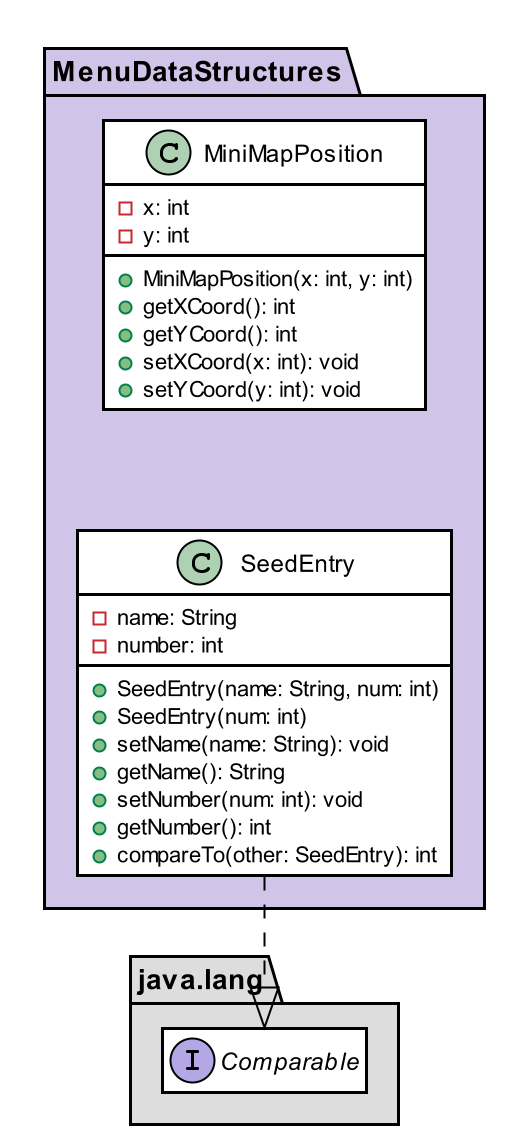
\includegraphics[width=.45\linewidth]{./GUI/GUI_Bilder/MenuDataStructures.png}
          \caption{Paket MenuDataStructures}
           \label{fig:MenuDataStructures}
\end{figure}
    \pagebreak
    \paragraph{\underline{MiniMapPosition}}\label{mmp} \mbox{}\\
        Diese Klasse stellt eine Datenstruktur für die 
        Positionen eines Spielers auf der MiniMap bereit.
        Sie besitzt eine X- und Y-Koordinate, sowie Getter
        und Setter.\\
        \par
        \textbf{Attribute}
        \begin{itemize}
            \item \textit{- int x}  
                \begin{leftbar}[0.9\linewidth]
                    Enthält die X-Koordinate eines Spielers auf 
                    der MiniMap.
                \end{leftbar}
            \item \textit{- int y} 
                \begin{leftbar}[0.9\linewidth]
                    Enthält die Y-Koordinate eines Spielers auf 
                    der MiniMap.
                \end{leftbar}
        \end{itemize}
        \textbf{Methoden}					
        \begin{itemize}
            \item \textit{+ MiniMapPosition(int x, int y)}
                \begin{leftbar}[0.9\linewidth]
                    Dieser Konstruktor speichert den übergebenen Namen und die 
                    Ziffernreihenfolge des neu erstellten Seed-Eintrag Objektes.\\
                    \textbf{@param x} Die zu setzende X-Koordinate.\\
                    \textbf{@param y} Die zu setzende Y-Koordinate.
                \end{leftbar}
            \item \textit{+ getXCoord(): int}
                \begin{leftbar}[0.9\linewidth]
                    Getter für die X-Koordinate eines Spielers auf 
                    der MiniMap.\\
                    \textbf{@return} Die X-Koordinate.
                \end{leftbar}
            \item \textit{+ getYCoord(): int}
                \begin{leftbar}[0.9\linewidth]
                    Getter für die Y-Koordinate eines Spielers auf 
                    der MiniMap.\\
                    \textbf{@return} Die Y-Koordinate.
                \end{leftbar}
            \item \textit{+ setXCoord(int x): void}
                \begin{leftbar}[0.9\linewidth]
                    Setter für die X-Koordinate eines Spielers auf 
                    der MiniMap.\\
                    \textbf{@param x} Die zu setzende X-Koordinate.
                \end{leftbar}
            \item \textit{+ setYCoord(int y): void}
                \begin{leftbar}[0.9\linewidth]
                    Setter für die Y-Koordinate eines Spielers auf 
                    der MiniMap.\\
                    \textbf{@param y} Die zu setzende Y-Koordinate.
                \end{leftbar}
        \end{itemize}

    \paragraph{\underline{SeedEntry}}\label{seedentry} \mbox{}\\
        Diese Klasse repräsentiert die Datenstruktur eines Seed Eintrages.
        Ein Seed Eintrag hat dabei immer einen Namen und eine Ziffernreihenfolge.
        Letzteres identifizert einen Seed Eintrag. Demzufolge können
        mehrere Seeds nicht die selbe Ziffernreihenfolge haben. Die Überprüfung
        findet jedoch nicht hier statt, sondern in den Menü Klassen aus dem GUI.
        Die Klasse implementiert das Comparable Interface, damit die Seed-Einträge
        später sortiert werden können.\\
        \par
        \pagebreak
        \textbf{Attribute}
        \begin{itemize}
            \item \textit{- String name}  
                \begin{leftbar}[0.9\linewidth]
                    Enthält den Namen vom Seed-Eintrag.
                \end{leftbar}
            \item \textit{- int number} 
                \begin{leftbar}[0.9\linewidth]
                    Enthält die Ziffernreihenfolge des Seed-Eintrages.
                \end{leftbar}
        \end{itemize}
        \textbf{Methoden}					
        \begin{itemize}
            \item \textit{+ SeedEntry(String name, int num)}
                \begin{leftbar}[0.9\linewidth]
                    Dieser Konstruktor speichert den übergebenen Namen und die 
                    Ziffernreihenfolge des neu erstellten Seed-Eintrag Objektes.\\
                    \textbf{@param name} Der zu setzende Name.\\
                    \textbf{@param num} Die zu setzende Ziffernreihenfolge.\\
                \end{leftbar}
            \item \textit{+ SeedEntry(int num)}
                \begin{leftbar}[0.9\linewidth]
                    Dieser Konstruktor speichert die Ziffernreihenfolge des neu 
                    erstellten Seed-Eintrag Objektes und setzt den Namen des 
                    Seed-Eintrages gleich der Ziffernreihenfolge.\\
                    \textbf{@param num} Die zu setzende Ziffernreihenfolge.\\
                \end{leftbar}
            \item \textit{+ setName(String name): void}
                \begin{leftbar}[0.9\linewidth]
                    Überschreibt den aktuellen Namen des Seed-Eintrages mit 
                    dem übergebenem String.\\
                    \textbf{@param name} Der zu speichernde Name.
                \end{leftbar}
            \item \textit{+ getName(): String}
                \begin{leftbar}[0.9\linewidth]
                    Gibt den aktuellen Namen des Seed-Eintrages zurück.\\
                    \textbf{@return} Name des Seed-Eintrages.
                \end{leftbar}
            \item \textit{+ setNumber(int num): void}
                \begin{leftbar}[0.9\linewidth]
                    Überschreibt die aktuelle Ziffernreihenfolge des Seed-Eintrages mit 
                    dem übergebenem Integer.\\
                    \textbf{@param num} Die zu speichernde Ziffernreihenfolge.\\
                \end{leftbar}
            \item \textit{+ getNumber(): int}
                \begin{leftbar}[0.9\linewidth]
                    Gibt die aktuelle Ziffernreihenfolge des Seed-Eintrages zurück.\\
                    \textbf{@return} Ziffernreihenfolge des Seed-Eintrages.
                \end{leftbar}
            \item \textit{+ compareTo(SeedEntry other): int}
                \begin{leftbar}[0.9\linewidth]
                    Siehe dazu java.lang.Comparable\#compareTo(java.lang.Object).
                \end{leftbar}
        \end{itemize}


\pagebreak

\subsubsection{menuconfig}\label{menuconfig}
    Dieses Paket verwaltet die Konfigurationsdateien für alle 
    Einstellungen, die im Einstellungsfenster des Menüs vorgenommen werden können.
    Dabei existiert für jede Dateei eine eigene Klasse. In den Klassen wird
    keine Einstellung durch den Benutzer vorgenommen. Es existieren lediglich
    Methoden, um die aktuellen eventuell veränderten Änderungen in die Datei 
    zu schreiben. Ebenfalls können die aktuell gespeicherten Dateien geladen
    und den anderen Klassen zur Verfügung gestellt werden. \par

    \begin{figure}[!h]
        \centering
        \centering
            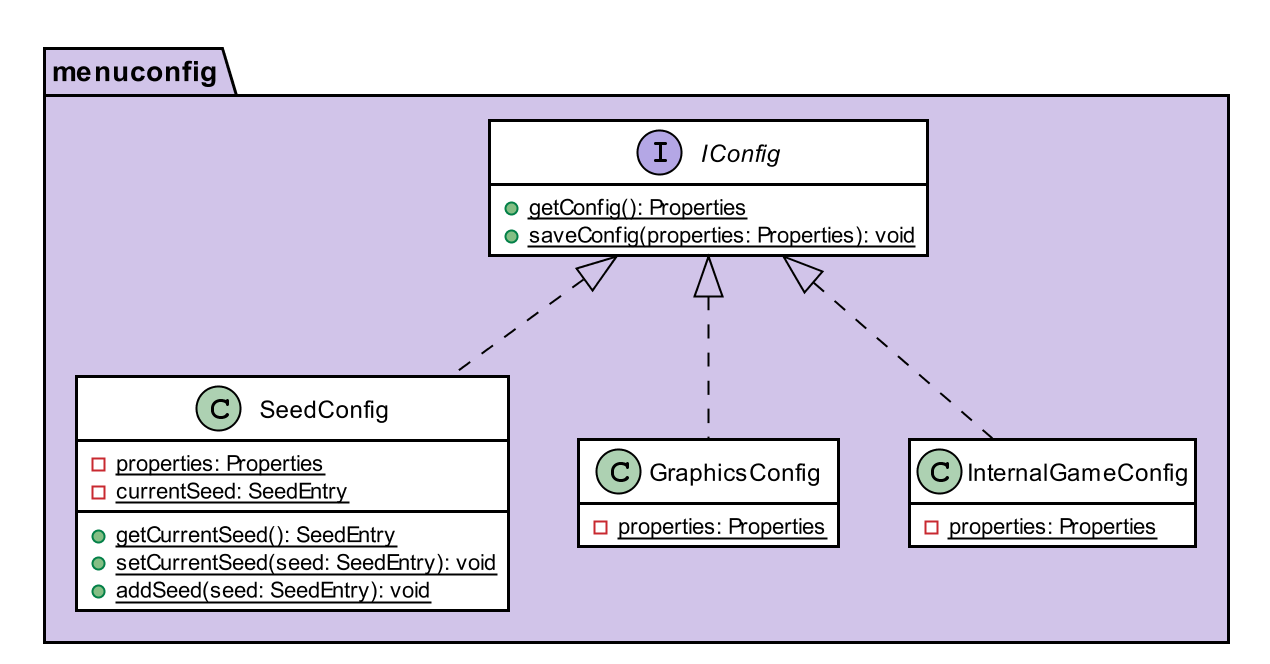
\includegraphics[width=\linewidth]{./GUI/GUI_Bilder/Config.png}
              \caption{Paket menuconfig}
               \label{fig:Config}
    \end{figure}

        \paragraph{\underline{IConfig}}\label{configlabel} \mbox{}\\
            Dieses Interface stellt Funktionen bereit, um Dateien zu laden und zu speichern.
            Jede Klasse die dieses Interface implementiert, muss die beiden Funktionen 
            überschreiben.

            \textbf{Methoden}					
            \begin{itemize}
                \item \textit{+ {static} getConfig(): Properties}
                    \begin{leftbar}[0.9\linewidth]
                        Gibt das Properties Objekt der Konfiguration zurück.\\
                        \textbf{@return} Das aktuelle Properties Objekt.
                    \end{leftbar}
                \item \textit{+ {static} saveConfig(Properties properties): void}
                    \begin{leftbar}[0.9\linewidth]
                        Überschreibt das aktuelle Properties Objekt mit dem übergebenem.\\
                        \textbf{@param properties} Das zu speichernde Properties Objekt.
                    \end{leftbar}
            \end{itemize}
            \pagebreak
        \paragraph{\underline{SeedConfig}} \mbox{}\\
            Diese Klasse verwaltet die Konfiguration der Seeds, bzw. speichert alle 
            vorhandenen Seeds in einer Datei, oder ergänzt diese um einen Seed. 
            Außerdem speichert sie den aktuell ausgewählten Seed.
            Ebenfalls wird das Interface~\nameref{configlabel} implementiert, um die Konfigurations Datei
            laden und speichern zu können. \par 
            \textbf{Attribute}
            \begin{itemize}
                \item \textit{- {static} Properties properties}
                    \begin{leftbar}[0.9\linewidth]
                        In diesem Properties Objekt werden die Einstellungen bzw Daten 
                        gespeichert.
                    \end{leftbar}
                \item \textit{- {static} currentSeedEntry: SeedEntry} 
                    \begin{leftbar}[0.9\linewidth]
                        Enthält den aktuell ausgewählten Seed.
                    \end{leftbar}
            \end{itemize}
            
            \textbf{Methoden}					
            \begin{itemize}
                \item \textit{+ {static} getCurrentSeed(): SeedEntry}
                    \begin{leftbar}[0.9\linewidth]
                        Gibt den aktuell ausgewählten Seed zurück.\\
                        \textbf{@return} Der aktuell ausgewählte Seed.
                    \end{leftbar}
                \item \textit{+ {static} setCurrentSeed(SeedEntry seed): void}
                    \begin{leftbar}[0.9\linewidth]
                        Überschreibt den aktuellen Seed mit einem neuen Seed Objekt.\\
                        \textbf{@param seed} Der zu speichernde Seed.
                    \end{leftbar}
                \item \textit{+ {static} addSeed(SeedEntry seed): void}
                    \begin{leftbar}[0.9\linewidth]
                        Fügt der SeedConfig Datei einen neuen Seed hinzu, wobei die 
                        Alten beibehalten werden.\\
                        \textbf{@param seed} Der Seed welcher hinzugefügt werden soll.
                    \end{leftbar}
            \end{itemize}

        \pagebreak
        \paragraph{\underline{GraphicsConfig}} \mbox{}\\
            Diese Klasse verwaltet die Konfiguration der im Menü einstellbaren 
            Grafikeinstellungen, bzw. speichert alle vorgenommen Änderungen der
            Grafik in einer Datei. 
            Ebenfalls wird das Interface~\nameref{configlabel} implementiert, um die Konfigurations Datei
            laden und speichern zu können. \par    
                    
            \textbf{Attribute}
            \begin{itemize}
                \item \textit{- {static} Properties properties}
                    \begin{leftbar}[0.9\linewidth]
                        In diesem Properties Objekt werden die Einstellungen bzw Daten 
                        gespeichert.
                    \end{leftbar}
            \end{itemize}
            
            \textbf{Methoden}					
            \begin{itemize}
                \item \textit{+ {static} getGraphicsConfig(): Properties}
                    \begin{leftbar}[0.9\linewidth]
                        Gibt das Properties Objekt der Grafik Konfiguration zurück.\\
                        \textbf{@return} Das aktuelle Properties Objekt.
                    \end{leftbar}
            \end{itemize}
		
		\paragraph{\underline{InternalGameConfig}} \mbox{}\\
            Diese Klasse verwaltet die Konfiguration der im Menü einstellbaren 
            internen Spieleinstellungen, bzw. speichert alle vorgenommen Änderungen
            in einer Datei. 
            Ebenfalls wird das Interface~\nameref{configlabel} implementiert, um die Konfigurations Datei
            laden und speichern zu können. \par    
                    
            \textbf{Attribute}
            \begin{itemize}
                \item \textit{- {static} Properties properties}
                    \begin{leftbar}[0.9\linewidth]
                        In diesem Properties Objekt werden die Einstellungen bzw Daten 
                        gespeichert.
                    \end{leftbar}
            \end{itemize}

    \pagebreak

\subsubsection{gui}\label{guipaket}
    Das gui Packet beinhaltet die Steuerungsklassen für alle grafischen
    Benutzeroberflächen des Spieles. Für jedes Menü existiert eine eigene
    Steuerungsklasse.
    Um Kontrolle über die Spieleapplikation zu haben existiert eine AppState Klasse, 
    welche von  \textit{com.jme3.app.state.AbstractAppState} erbt. Dies beinhaltet 
    die Bereitstellung der Information, ob und wenn ja,was für ein Menü-Bildschirm 
    geöffnet ist. Von dieser AppState Klasse erben weiterhin alle Steuerungsklassen, 
    die Zugriff auf die Applikation benötigen.
    Um auf Benuztereingaben und -aktionen reagieren zu können, wird ein
    Eingabe Mapping implementiert. \par

    \begin{center}
        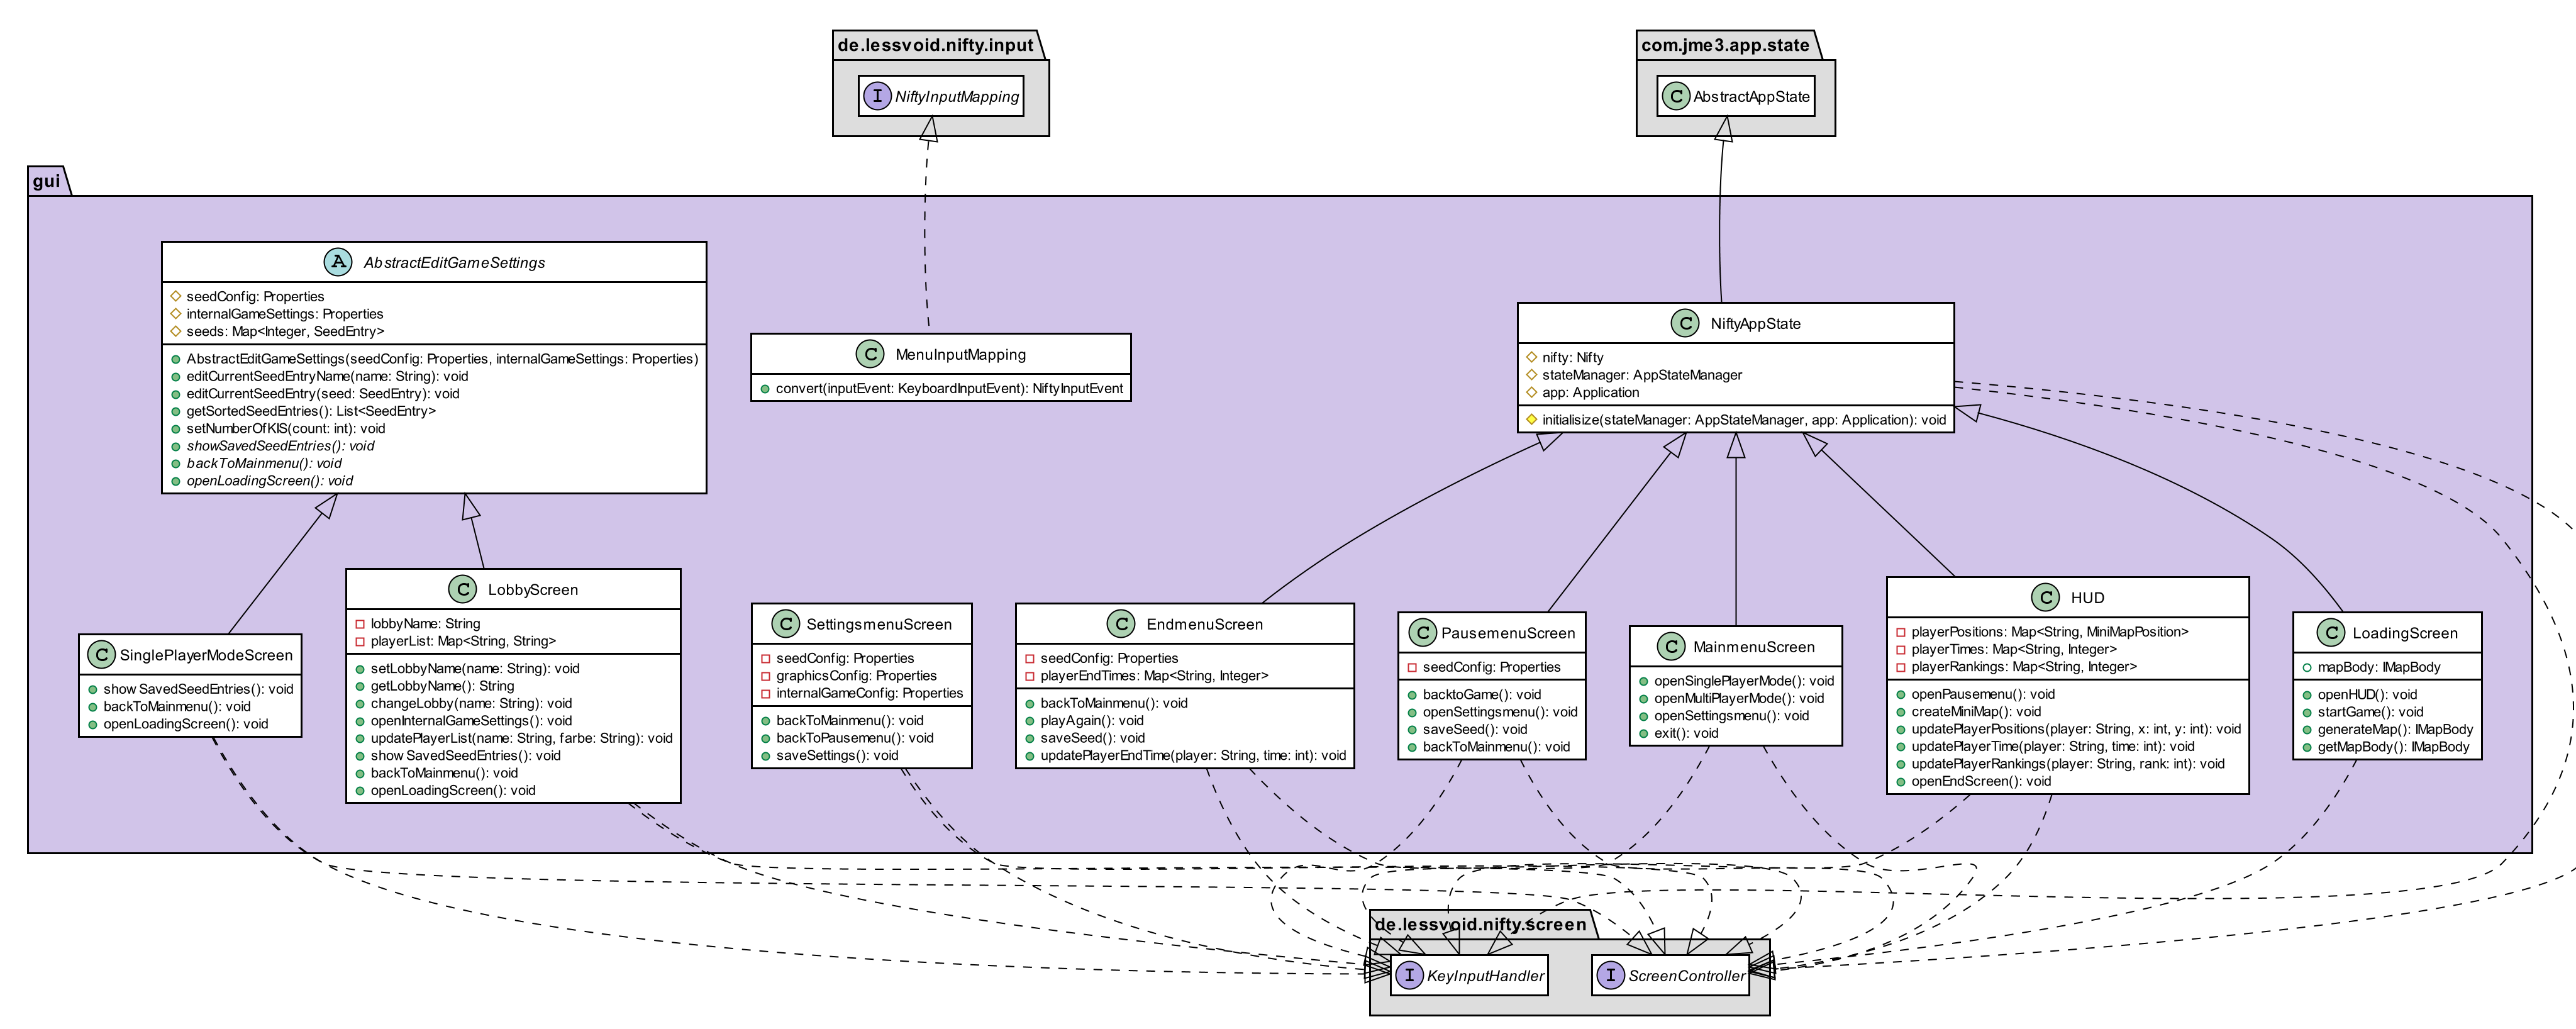
\includegraphics[width=0.85\linewidth]{./GUI/GUI_Bilder/GUI.png}
        \captionof{figure}{Paket gui}
        \label{fig:gui}
    \end{center}

        \pagebreak
        \paragraph{\underline{NiftyAppState}}\label{nas} \mbox{}\\
            Diese Klasse dient als Oberklasse für die meisten Steuerungsklassen 
            der grafischen Benutzeroberfläche des Spieles. Sie erbt von 
            \textit{com.jme3.app.state.AbstractAppState}, um Kontrolle über die 
            Spieleapplikation zu haben. Dies beinhaltet  die Bereitstellung der
            Information, ob und wenn ja, was für ein Menü-Bildschirm geöffnet ist. 
            Dazu wird zu gegebenem Anlass der jeweilige Menü-Bildschirm vom/an den
            StateManager entfernt/hinzugefügt.\\
            Um die Bildschirme steuern zu können, wird das Interface
            \textit{de.lessvoid.nifty.screen.ScreenController} implementiert und um auf
            Benuztereingaben und -aktionen reagieren zu können das Interface
            \textit{de.lessvoid.nifty.screen.KeyInputHandler}. Hierzu wird,
            auf die in der Klasse \textit{MenuInputMapping} bereits konvertierten
            Eingaben in NiftyInputEvents, entsprechend reagiert.\\ \par
            \textbf{Attribute}
            \begin{itemize}
                \item  \textit{\# Nifty nifty}
                    \begin{leftbar}[0.9\linewidth]
                        Referenz auf das Nifty Objekt.
                    \end{leftbar}
                \item  \textit{\# AppStateManager stateManager}  
                    \begin{leftbar}[0.9\linewidth]
                        Referenz auf den AppStateManager der Applikation.
                    \end{leftbar}
                \item  \textit{\# Application app} 
                    \begin{leftbar}[0.9\linewidth]
                        Referenz auf die Applikation.
                    \end{leftbar}
            \end{itemize}
            \textbf{Methoden}					
            \begin{itemize}
                \item  \textit{\# initialisize(AppStateManager stateManager, Application app): void} 
                    \begin{leftbar}[0.9\linewidth]
                        Initialisiert die Attribute und ruft explizit den Konstruktor
                        von AbstractAppState auf. \\
                        \textbf{@param stateManager} Der StateManager, welcher verwendet werden
                        soll.\\
                        \textbf{@param app} Die Applikation, welche verwendet werden
                        soll.\\
                    \end{leftbar}
            \end{itemize}

        \pagebreak
        \paragraph{\underline{MenuInputMapping}}\label{mim} \mbox{}\\
            Diese Klasse ist zuständig für die Konvertierung von Benuztereingaben
            und -aktionen in NiftyInputEvents. Sie ersetzt damit die von Nifty automatisch
            bereitgestellte MenuInputMapping Klasse.\\
            Um dies zu erreichen, wird das Interface 
            \textit{de.lessvoid.nifty.input.NiftyInputMapping} implementiert.
            Da die Steuerungsklassen nur von NiftyInputEvents abhängen, kann so mit wenigem
            Aufwand andere Geräte wie GamePads integriert werden. Dazu muss nur das Mapping
            erweitert werden.
            \par
                    
            \textbf{Methoden}					
            \begin{itemize}
                \item  \textit{+ convert(KeyboardInputEvent inputEvent): NiftyInputEvent} 
                    \begin{leftbar}[0.9\linewidth]
                        Erhält ein KeyboardInputEvent und konvertiert es in ein
                        NiftyInputEvent. Dieses NiftyInputEvent wird dann weiter 
                        geleitet an die Steuerungsklassen der grafischen 
                        Benutzeroberflächen. Die Escape, Enter und Pfeil-Tasten 
                        werden hier gemappt.\\
                        \textbf{@param inputEvent} Die Taste, welche auf der Tastatur
                        gedrückt wird.\\
                        \textbf{@return} Das gemappte NiftyInputEvent.
                    \end{leftbar}
            \end{itemize}
        
        \paragraph{\underline{AbstractEditGameSettings}}\label{adgs} \mbox{}\\
            Diese Klasse dient als Oberklasse für die Steuerungsklassen des
            Einzelspielermodus und Lobby Bildschirmes. Es enthält zwei abstrakte 
            Methoden, die von den erbenden Klassen implementiert werden müssen.
            In dieser Klasse werden interne Spieleeinstellungen vorgenommen, 
            wie Einstellung der Anzahl an KI's. Außerdem kann man 
            Seeds ändern und hinzufügen. \par
            
            \textbf{Attribute}
            \begin{itemize}
                \item \textit{\# Properties seedConfig}  
                    \begin{leftbar}[0.9\linewidth]
                        Referenz auf das Properties Objekt der Seed Konfiguration.
                    \end{leftbar}
                \item  \textit{\# Properties internalGameSettings} 
                    \begin{leftbar}[0.9\linewidth]
                        Referenz auf das Properties Objekt der internen 
                        Spieleeinstellungen.
                    \end{leftbar}
                \item  \textit{\# Map<Integer, SeedEntry> seeds} 
                    \begin{leftbar}[0.9\linewidth]
                        HashMap die alle gespeicherten Seeds des Spieles 
                        enthält. Dabei wird die Integer Zahlrenreihenfolge
                        des Seeds als Key gespeichert, damit dieser Unique
                        bleibt.
                    \end{leftbar}
            \end{itemize}
               
            \textbf{Methoden}					
            \begin{itemize}
                \item  \textit{+ AbstractEditGameSettings(Properties seedConfig, Properties internalGameSettings)} 
                    \begin{leftbar}[0.9\linewidth]
                        Konstruktor der die Attribute der Klasse initalisiert mit den
                        übergenen Parametern und die Map als HashMap initalisiert.\\
                        \textbf{@param seedConfig} Properties Objekt der Seed 
                        Konfiguration.\\
                        \textbf{@param internalGameSettings} Properties Objekt der 
                        internen Spieleeinstellungen.
                    \end{leftbar}
                \pagebreak
                \item  \textit{+ editCurrentSeedEntryName(String name): void} 
                    \begin{leftbar}[0.9\linewidth]
                        Überschreibt den Namen des aktuell ausgewählten
                        Seeds mit dem übergebenem String.\\
                        \textbf{@param name} Der zu speichernde String.\\
                    \end{leftbar}
                \item  \textit{+ editCurrentSeedEntry(SeedEntry seed): void} 
                    \begin{leftbar}[0.9\linewidth]
                        Überschreibt den aktuell ausgewählten Seed mit dem
                        übergebenem Seed.\\
                        \textbf{@param seed} Der zu speichernde Seed.\\
                    \end{leftbar}
                \item  \textit{+ getSortedSeedEntries(): List<SeedEntry>}
                    \begin{leftbar}[0.9\linewidth]
                        Gibt eine nach Namen sortierte SeedEntry Liste zurück.\\
                        \textbf{@return} Die sortierte SeedEntry Liste.
                    \end{leftbar}
                \item  \textit{+ setNumberOfKIS(int count): void} 
                    \begin{leftbar}[0.9\linewidth]
                        Setzt die Anzahl der KI's entsprechend der noch verfügbaren 
                        Plätze. Wenn 10 Spieler das Spiel spielen möchten, so kann 
                        keine KI hinzugefügt werden.\\
                        \textbf{@param count} Die zu setzende Anzahl an KI's.\\
                    \end{leftbar}
                \item  \textit{+ {abstract} showSavedSeeds(): void} 
                    \begin{leftbar}[0.9\linewidth]
                        Füllt das im Fenster anzuzeigende DropDown Menü mit den im Spiel
                        gespeicherten Seeds. Dazu wird die Methode \textit{getSortedSeedEntries()} aus
                        der selben Klasse aufgerufen. \\
                    \end{leftbar}
                \item  \textit{+ {abstract} backToMainmenu(): void} 
                    \begin{leftbar}[0.9\linewidth]
                        Kehrt aus dem aktuellen Fenster zum Hauptmenü zurück.\\
                    \end{leftbar}
                \item  \textit{+ {abstract} openLoadingScreen(): void} 
                    \begin{leftbar}[0.9\linewidth]
                        Geht aus dem aktuellen Fenster zum Lade Bildschirm.\\
                    \end{leftbar}
            \end{itemize}
        
        \pagebreak
		\paragraph{\underline{SinglePlayerModeScreen}} \mbox{}\\
            Diese Klasse dient der Steuerung der grafischen Benutzeroberfläche
            des Einzelmodus Bildschirmes. Sie setzt alle Klicks und Eingaben
            um und führt sie aus. Dazu erbt sie von~\nameref{adgs}, denn dort
            sind passende Methoden bereits implementiert und aufgelistet.\\
            Um die Bildschirme steuern zu können, wird das Interface
            \textit{de.lessvoid.nifty.screen.ScreenController} implementiert und um auf
            Benuztereingaben und -aktionen reagieren zu können das Interface
            \textit{de.lessvoid.nifty.screen.KeyInputHandler}.  \par

            \textbf{Methoden}					
            \begin{itemize}
                \item  \textit{+ showSavedSeeds(): void} 
                    \begin{leftbar}[0.9\linewidth]
                        Füllt das im Fenster anzuzeigende DropDown Menü mit den im Spiel
                        gespeicherten Seeds. Dazu wird die Methode \textit{getSortedSeedEntries()} aus
                        der geerbten Klasse aufgerufen. \\
                    \end{leftbar}
                \item  \textit{+ backToMainmenu(): void} 
                    \begin{leftbar}[0.9\linewidth]
                        Kehrt aus dem aktuellen Fenster zum Hauptmenü zurück.\\
                    \end{leftbar}
                \item  \textit{+ openLoadingScreen(): void} 
                    \begin{leftbar}[0.9\linewidth]
                        Geht aus dem aktuellen Fenster zum Lade Bildschirm.\\
                    \end{leftbar}
            \end{itemize}        
        
        \paragraph{\underline{LobbyScreen}} \mbox{}\\
            Diese Klasse dient der Steuerung der grafischen Benutzeroberfläche
            des Lobby Bildschirmes. Sie setzt alle Klicks und Eingaben
            um und führt sie aus. Dazu erbt sie von~\nameref{adgs}, denn dort
            sind passende Methoden bereits implementiert und aufgelistet.\\
            Um die Bildschirme steuern zu können, wird das Interface
            \textit{de.lessvoid.nifty.screen.ScreenController} implementiert und um auf
            Benuztereingaben und -aktionen reagieren zu können das Interface
            \textit{de.lessvoid.nifty.screen.KeyInputHandler}. \par
            
            \textbf{Attribute}
            \begin{itemize}
                \item \textit{- String lobbyName}  
                    \begin{leftbar}[0.9\linewidth]
                        Speichert den Namen der Lobby in der sich der Spieler 
                        aktuell befindet.\\
                    \end{leftbar}
                \item  \textit{- Map<String, String> playerList} 
                    \begin{leftbar}[0.9\linewidth]
                        Speichert alle Spieler, die der Lobby beigetreten sind 
                        sowie deren Farben als Hashmap.
                    \end{leftbar}
            \end{itemize}
               
            \textbf{Methoden}					
            \begin{itemize}
                \item  \textit{+ setLobbyName(String name): void} 
                    \begin{leftbar}[0.9\linewidth]
                        Überschreibt den Lobbynamen der aktuell 
                        beigetreten Lobby.\\
                        \textbf{@param name} Der zu speichernde Lobby Name.\\
                    \end{leftbar}
                \item  \textit{+ getLobbyName(): String} 
                    \begin{leftbar}[0.9\linewidth]
                        Gibt den Namen derjenigen Lobby zurück, in der 
                        sich der Spieler aktuell befindet.\\
                        \textbf{return} Der Lobby Name.\\
                    \end{leftbar}
                \item  \textit{+ changeLobby(String name): void} 
                    \begin{leftbar}[0.9\linewidth]
                        Wechselt die Lobby durch Eingabe eines anderen 
                        Lobby Namens. Existiert dieser nicht, kann 
                        auch nicht gewechselt werden.\\
                        \textbf{@param name} Der Namme der Lobby, zu der 
                        man wechseln möchte.\\
                    \end{leftbar}
                \item  \textit{+ openInternalGameSettings(): void} 
                    \begin{leftbar}[0.9\linewidth]
                        Öffnet ein Popup, in der die internen Spieleeinstellungen 
                        vorgenommen werden können.
                    \end{leftbar}
                \item  \textit{+ updatePlayerList(String name, String farbe): void} 
                    \begin{leftbar}[0.9\linewidth]
                        Sobald ein weiterer Spieler die Lobby betritt, 
                        aktualisiert sich die Hashmap.\\
                        \textbf{@param name} Der Name des neuen Spielers.\\
                        \textbf{@param farbe} Die Farbe des neuen Spielers, welche 
                        vom System selber gesetzt wird. Der Spieler hat darauf 
                        keinen Einfluss.\\
                    \end{leftbar}
                \item  \textit{+ showSavedSeeds(): void} 
                    \begin{leftbar}[0.9\linewidth]
                        Füllt das im Popup-Fenster anzuzeigende DropDown Menü mit den im Spiel
                        gespeicherten Seeds. Dazu wird die Methode \textit{getSortedSeedEntries()} aus
                        der geerbten Klasse aufgerufen. \\
                    \end{leftbar}
                \item  \textit{+ backToMainmenu(): void} 
                    \begin{leftbar}[0.9\linewidth]
                        Kehrt aus dem aktuellen Fenster zum Hauptmenü zurück.\\
                    \end{leftbar}
                \item  \textit{+ openLoadingScreen(): void} 
                    \begin{leftbar}[0.9\linewidth]
                        Geht aus dem aktuellen Fenster zum Lade Bildschrim.\\
                    \end{leftbar}
            \end{itemize}

        \pagebreak
        \paragraph{\underline{LoadingScreen}} \mbox{}\\
        Diese Klasse dient der Steuerung der grafischen Benutzeroberfläche
        des Lade Bildschirmes. Sie erbt von~\nameref{nas}, um Kontrolle über die 
        Spieleapplikation zu haben. Dies beinhaltet  die Bereitstellung der
        Information, ob und wenn ja, was für ein Menü-Bildschirm geöffnet ist.
        Dazu wird zu gegebenem Anlass der jeweilige Menü-Bildschirm vom/an den
        StateManager entfernt/hinzugefügt.\\
        Um die Bildschirme steuern zu können, wird das Interface
        \textit{de.lessvoid.nifty.screen.ScreenController} implementiert. \par
            
            \textbf{Attribute}
            \begin{itemize}
                \item \textit{+ IMapBody mapBody}  
                    \begin{leftbar}[0.9\linewidth]
                        Schnittstelle für das andere Team des PSE-Projektes.
                        Hier wird der Output des Strecken-Generatos gespeichert.
                    \end{leftbar}
            \end{itemize}
               
            \textbf{Methoden}					
            \begin{itemize}
                \item  \textit{+ openHUD(): void} 
                    \begin{leftbar}[0.9\linewidth]
                        Öffnet den Bildschirm des HUD's.\\
                    \end{leftbar}
                \item  \textit{+ startGame(): void} 
                    \begin{leftbar}[0.9\linewidth]
                        Hier werden alle AppStates, die während dem Rennen 
                        laufen sollen, initalisiert bzw an den AppStateManager
                        angehängt.
                    \end{leftbar}
                \item  \textit{+ generateMap(): IMapBody} 
                    \begin{leftbar}[0.9\linewidth]
                        Hier wird der Strecken-Generator aufgerufen, der dann 
                        einen Output liefert, welcher im Attribut mapBody 
                        gespeichert wird.
                    \end{leftbar}
                \item  \textit{+ getIMapBody(): IMapBody} 
                    \begin{leftbar}[0.9\linewidth]
                        Getter für das Attribut IMapBody.
                    \end{leftbar}
            \end{itemize}

		\paragraph{\underline{MainmenuScreen}} \mbox{}\\
            Diese Klasse dient der Steuerung der grafischen Benutzeroberfläche
            des Hauptmenü Bildschirmes. Sie erbt von~\nameref{nas}, um Kontrolle über die 
            Spieleapplikation zu haben. Dies beinhaltet  die Bereitstellung der
            Information, ob und wenn ja, was für ein Menü-Bildschirm geöffnet ist.
            Dazu wird zu gegebenem Anlass der jeweilige Menü-Bildschirm vom/an den
            StateManager entfernt/hinzugefügt.\\
            Um die Bildschirme steuern zu können, wird das Interface
            \textit{de.lessvoid.nifty.screen.ScreenController} implementiert und um auf
            Benuztereingaben und -aktionen reagieren zu können das Interface
            \textit{de.lessvoid.nifty.screen.KeyInputHandler}. \par
                        
            \textbf{Methoden}					
            \begin{itemize}
                \item  \textit{+ openSinglePlayerMode(): void} 
                    \begin{leftbar}[0.9\linewidth]
                        Wechselt zu dem Einzelspielermodus Bildschirm.\\
                    \end{leftbar}
                    \pagebreak
                \item  \textit{+ openMultiPlayerMode(): void} 
                    \begin{leftbar}[0.9\linewidth]
                        Wechselt zu dem Lobby Bildschirm.\\
                    \end{leftbar}
                \item  \textit{+ openSettingsmenu(): void} 
                    \begin{leftbar}[0.9\linewidth]
                        Wechselt zu dem Einstellungen Bildschirm.\\
                    \end{leftbar}
                \item  \textit{+ exit(): void} 
                    \begin{leftbar}[0.9\linewidth]
                        Beendet die Applikation.\\
                    \end{leftbar}
            \end{itemize}
        
        

        \paragraph{\underline{HUD}} \mbox{}\\
            Diese Klasse dient der Steuerung des HUD
            während des Rennens. Sie erbt von~\nameref{nas}, um Kontrolle über die 
            Spieleapplikation zu haben. Dies beinhaltet  die Bereitstellung der
            Information, ob und wenn ja, was für ein Menü-Bildschirm geöffnet ist.
            Dazu wird zu gegebenem Anlass der jeweilige Menü-Bildschirm vom/an den
            StateManager entfernt/hinzugefügt.\\
            Um die Bildschirme steuern zu können, wird das Interface
            \textit{de.lessvoid.nifty.screen.ScreenController} implementiert und um auf
            Benuztereingaben und -aktionen reagieren zu können das Interface
            \textit{de.lessvoid.nifty.screen.KeyInputHandler}. \par
            
            \textbf{Attribute}
            \begin{itemize}
                \item \textit{- Map<String, MiniMapPosition> playerPositions}  
                    \begin{leftbar}[0.9\linewidth]
                        Hashmap, welche zu jedem Spieler die aktuelle MiniMap-Position speichert.
                    \end{leftbar}
                \item  \textit{- Map<String, Integer> playerTimes} 
                    \begin{leftbar}[0.9\linewidth]
                        Hashmap, welche zu jedem Spieler seine bisher gefahrene Zeit enthält.
                    \end{leftbar}
                \item  \textit{- Map<String, Integer> playerRankings} 
                    \begin{leftbar}[0.9\linewidth]
                        Hashmap, welche zu jedem Spieler die Platzierung speichert.
                    \end{leftbar}
            \end{itemize}
               
            \textbf{Methoden}					
            \begin{itemize}
                \item  \textit{+ openPausemenu(): void} 
                    \begin{leftbar}[0.9\linewidth]
                        Öffnet das Pausemenü.\\
                    \end{leftbar}
                \item  \textit{+ createMiniMap(): void} 
                    \begin{leftbar}[0.9\linewidth]
                        Erstellt eine MiniMap, welche im HUD angezeigt werden soll.\\
                    \end{leftbar}
                    \pagebreak
                \item  \textit{+ updatePlayerPositions(String player, int x, int y): void} 
                    \begin{leftbar}[0.9\linewidth]
                        Aktualisiert die Position eines Spielers mit den gegebenen Koordinaten.\\
                        \textbf{@param player} Der Spieler, dessen Koordinaten aktualisiert
                        werden sollen.\\
                        \textbf{@param x} X-Koordinate des Spielers.\\
                        \textbf{@param y} Y-Koordinate des Spielers.\\
                    \end{leftbar}
                \item  \textit{+ updatePlayerTime(String player, int time): void} 
                    \begin{leftbar}[0.9\linewidth]
                        Aktualisiert die Zeit eines Spielers mit dem übergebenem Integer.\\
                        \textbf{@param player} Der Spieler, dessen zeit aktualisiert werden soll.\\
                        \textbf{@param time} Die neue Zeit des Spielers.\\
                    \end{leftbar}
                \item  \textit{+ updatePlayerRankings(String player, int rank): void} 
                    \begin{leftbar}[0.9\linewidth]
                        Aktualisiert die Platzierung des Spielers mit dem übergebenem Integer.\\
                        \textbf{@param player} Der Spieler, dessen Platzierung aktualisiert werden soll.\\
                        \textbf{@param rank} Die neue Platzierung des Spielers.\\
                    \end{leftbar}
                \item  \textit{+ openEndScreen(): void} 
                    \begin{leftbar}[0.9\linewidth]
                        Öffnet den Endmenü Bildschirm.\\
                    \end{leftbar}
            \end{itemize}

        \paragraph{\underline{PausemenuScreen}} \mbox{}\\
            Diese Klasse dient der Steuerung der grafischen Benutzeroberfläche
            des Pausemenü Bildschirmes. Sie erbt von~\nameref{nas}, um Kontrolle über die 
            Spieleapplikation zu haben. Dies beinhaltet  die Bereitstellung der
            Information, ob und wenn ja, was für ein Menü-Bildschirm geöffnet ist.
            Dazu wird zu gegebenem Anlass der jeweilige Menü-Bildschirm vom/an den
            StateManager entfernt/hinzugefügt.\\
            Um die Bildschirme steuern zu können, wird das Interface
            \textit{de.lessvoid.nifty.screen.ScreenController} implementiert und um auf
            Benuztereingaben und -aktionen reagieren zu können das Interface
            \textit{de.lessvoid.nifty.screen.KeyInputHandler}. \par
                
            \textbf{Attribute}
            \begin{itemize}
                \item \textit{- Properties seedConfig}  
                    \begin{leftbar}[0.9\linewidth]
                        Referenz auf das Properties Objekt der Seed Konfiguration.
                    \end{leftbar}
            \end{itemize}

            \textbf{Methoden}					
            \begin{itemize}
                \item  \textit{+ backtoGame(): void} 
                    \begin{leftbar}[0.9\linewidth]
                        Kehrt zum Spiel zurück.\\
                    \end{leftbar}
                \item  \textit{+ openSettingsmenu(): void} 
                    \begin{leftbar}[0.9\linewidth]
                        Öffnet das Einstellungsfenster.\\
                    \end{leftbar}
                \item  \textit{+ saveSeed(): void} 
                    \begin{leftbar}[0.9\linewidth]
                        Speichert einen Seed.\\
                    \end{leftbar}
                \item  \textit{+ backToMainmenu(): void} 
                    \begin{leftbar}[0.9\linewidth]
                        Kehrt zum Hauptmenü des Spieles zurück.\\
                    \end{leftbar}
            \end{itemize}

        
        \paragraph{\underline{SettingsmenuScreen}} \mbox{}\\
            Diese Klasse dient der Steuerung der grafischen Benutzeroberfläche
            des Einstellungs Bildschirmes. Sie erbt von~\nameref{nas}, um Kontrolle über die 
            Spieleapplikation zu haben. Dies beinhaltet  die Bereitstellung der
            Information, ob und wenn ja, was für ein Menü-Bildschirm geöffnet ist.
            Dazu wird zu gegebenem Anlass der jeweilige Menü-Bildschirm vom/an den
            StateManager entfernt/hinzugefügt.
            Um die Bildschirme steuern zu können, wird das Interface\\
            \textit{de.lessvoid.nifty.screen.ScreenController} implementiert und um auf
            Benuztereingaben und -aktionen reagieren zu können das Interface
            \textit{de.lessvoid.nifty.screen.KeyInputHandler}. \par
            
            \textbf{Attribute}
            \begin{itemize}
                \item \textit{- Properties seedConfig}  
                    \begin{leftbar}[0.9\linewidth]
                        Referenz auf das Properties Objekt der Seed Konfiguration.
                    \end{leftbar}
                \item  \textit{- Properties graphicsConfig} 
                    \begin{leftbar}[0.9\linewidth]
                        Referenz auf das Properties Objekt der Grafik Konfiguration.
                    \end{leftbar}
                \item  \textit{- Properties internalGameConfig} 
                    \begin{leftbar}[0.9\linewidth]
                        Referenz auf das Properties Objekt der internen Spiel Konfiguration.
                    \end{leftbar}
            \end{itemize}
               
            \textbf{Methoden}					
            \begin{itemize}
                \item  \textit{+ backToMainmenu(): void} 
                    \begin{leftbar}[0.9\linewidth]
                        Kehrt zum Hauptmenü zurück.\\
                    \end{leftbar}
                \item  \textit{+ backToPausemenu(): void} 
                    \begin{leftbar}[0.9\linewidth]
                        Kehrt zum Pausemenü zurück.\\
                    \end{leftbar}
                \item  \textit{+ saveSettings(): void} 
                    \begin{leftbar}[0.9\linewidth]
                        Speichert die Einstellungen.\\
                    \end{leftbar}
            \end{itemize}

        \pagebreak
        \paragraph{\underline{EndmenuScreen}} \mbox{}\\
        Diese Klasse dient der Steuerung der grafischen Benutzeroberfläche
        des Endmenü Bildschirmes. Sie erbt von~\nameref{nas}, um Kontrolle über die 
        Spieleapplikation zu haben. Dies beinhaltet  die Bereitstellung der
        Information, ob und wenn ja, was für ein Menü-Bildschirm geöffnet ist. \par
        Dazu wird zu gegebenem Anlass der jeweilige Menü-Bildschirm vom/an den
        StateManager entfernt/hinzugefügt.
        Um die Bildschirme steuern zu können, wird das Interface\\
        \textit{de.lessvoid.nifty.screen.ScreenController} implementiert und um auf
        Benuztereingaben und -aktionen reagieren zu können das Interface
        \textit{de.lessvoid.nifty.screen.KeyInputHandler}.\par
            
            \textbf{Attribute}
            \begin{itemize}
                \item \textit{- Properties seedConfig}  
                    \begin{leftbar}[0.9\linewidth]
                        Referenz auf das Properties Objekt der Seed Konfiguration.
                    \end{leftbar}
                \item  \textit{- Map<String, Integer> playerEndTimes} 
                    \begin{leftbar}[0.9\linewidth]
                        Hashmap, welche die endgültig gefahrenen Zeiten der Spieler enthält.
                    \end{leftbar}
            \end{itemize}
               
            \textbf{Methoden}					
            \begin{itemize}
                \item  \textit{+ backToMainmenu(): void} 
                    \begin{leftbar}[0.9\linewidth]
                        Kehrt zum Hauptmenü zurück.\\
                    \end{leftbar}
                \item  \textit{+ playAgain(): void} 
                    \begin{leftbar}[0.9\linewidth]
                        Ein erneutes Spiel wird gestartet, mit der selben Konfgiruation 
                        und Strecke.\\
                    \end{leftbar}
                \item  \textit{+ saveSeed(): void} 
                    \begin{leftbar}[0.9\linewidth]
                        Speichert den Seed.\\
                    \end{leftbar}
                \item  \textit{+ updatePlayerEndTime(String player, int time): void} 
                    \begin{leftbar}[0.9\linewidth]
                        Sobald ein Spieler ins Ziel gekommen ist, wird dieser dieser Hashmap 
                        hinzugefügt mit seiner gefahrenen Zeit.\\
                        \textbf{@param player} Der Spieler, welcher ins Ziel gekommen ist.\\
                        \textbf{@param time} Des Spielers gefahrene Zeit.\\
                    \end{leftbar}
            \end{itemize}
    \pagebreak
	\pagebreak
	
	\section{Sequenzdiagramme}

		\subsection{InGame - Grafik}

\begin{figure}[htbp]
    \centering
    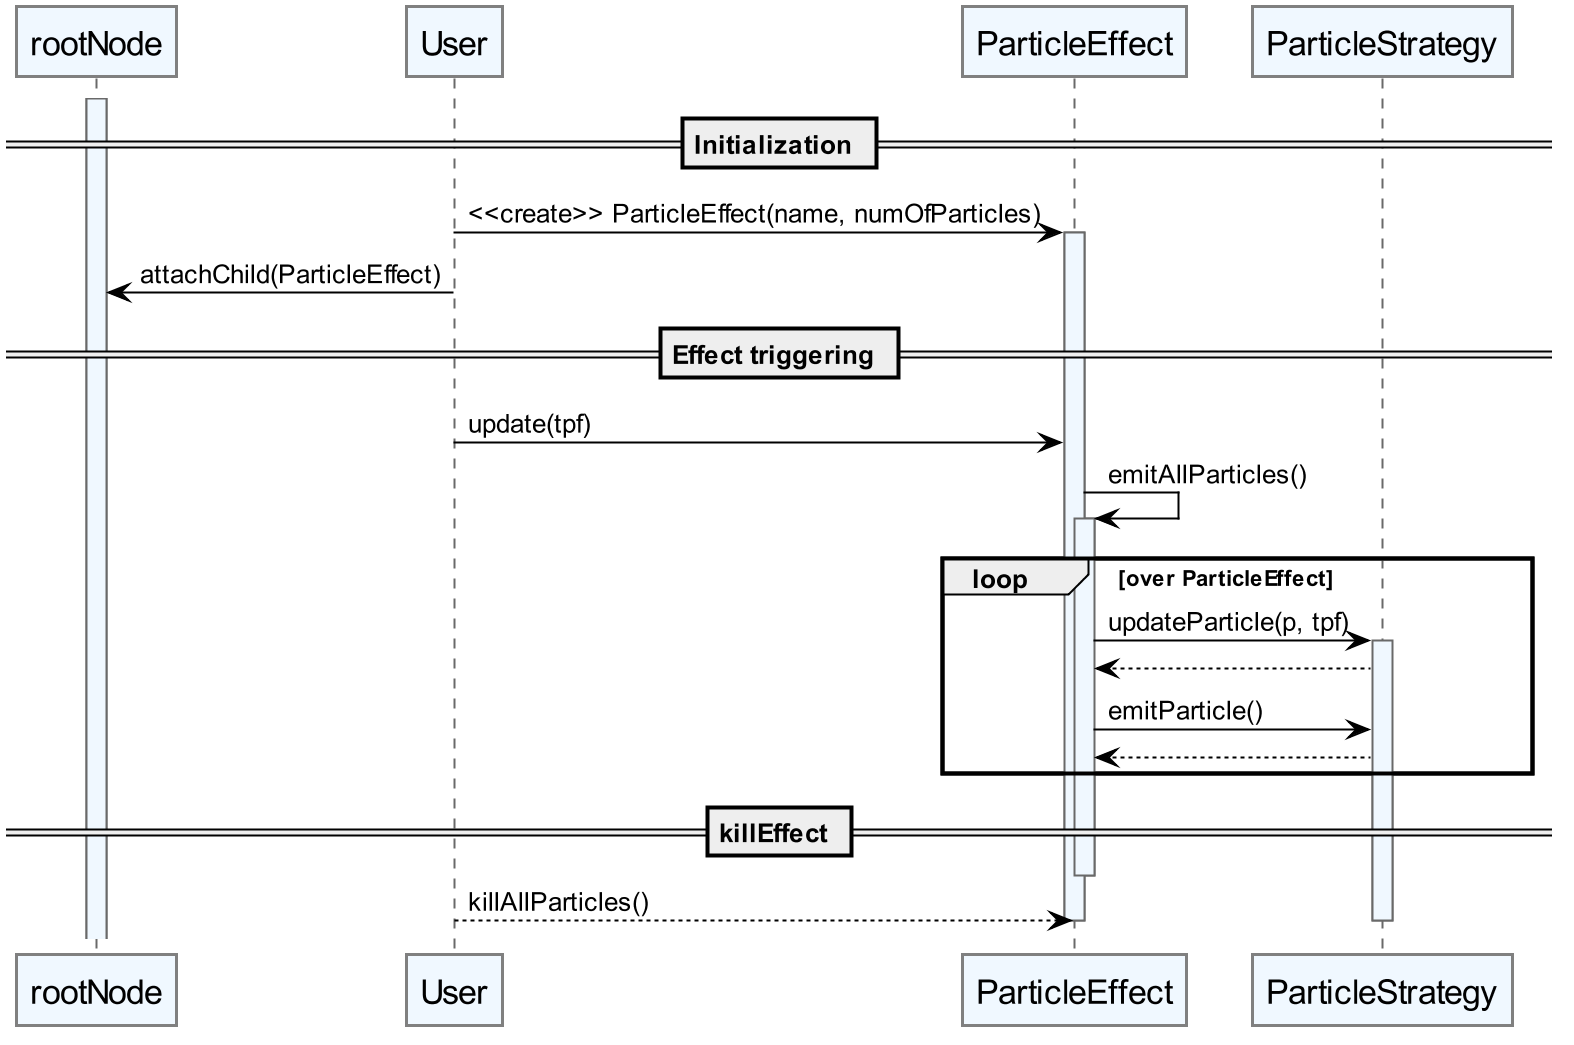
\includegraphics[width=1\linewidth]{InGameGrafik/Bilder/particleEmitterSequence.png}
    \caption{Sequenzdiagram effects}
\end{figure}
		\pagebreak
		\subsection{InGame - Interface}

\subsubsection{tick.Tick}

\begin{center}
    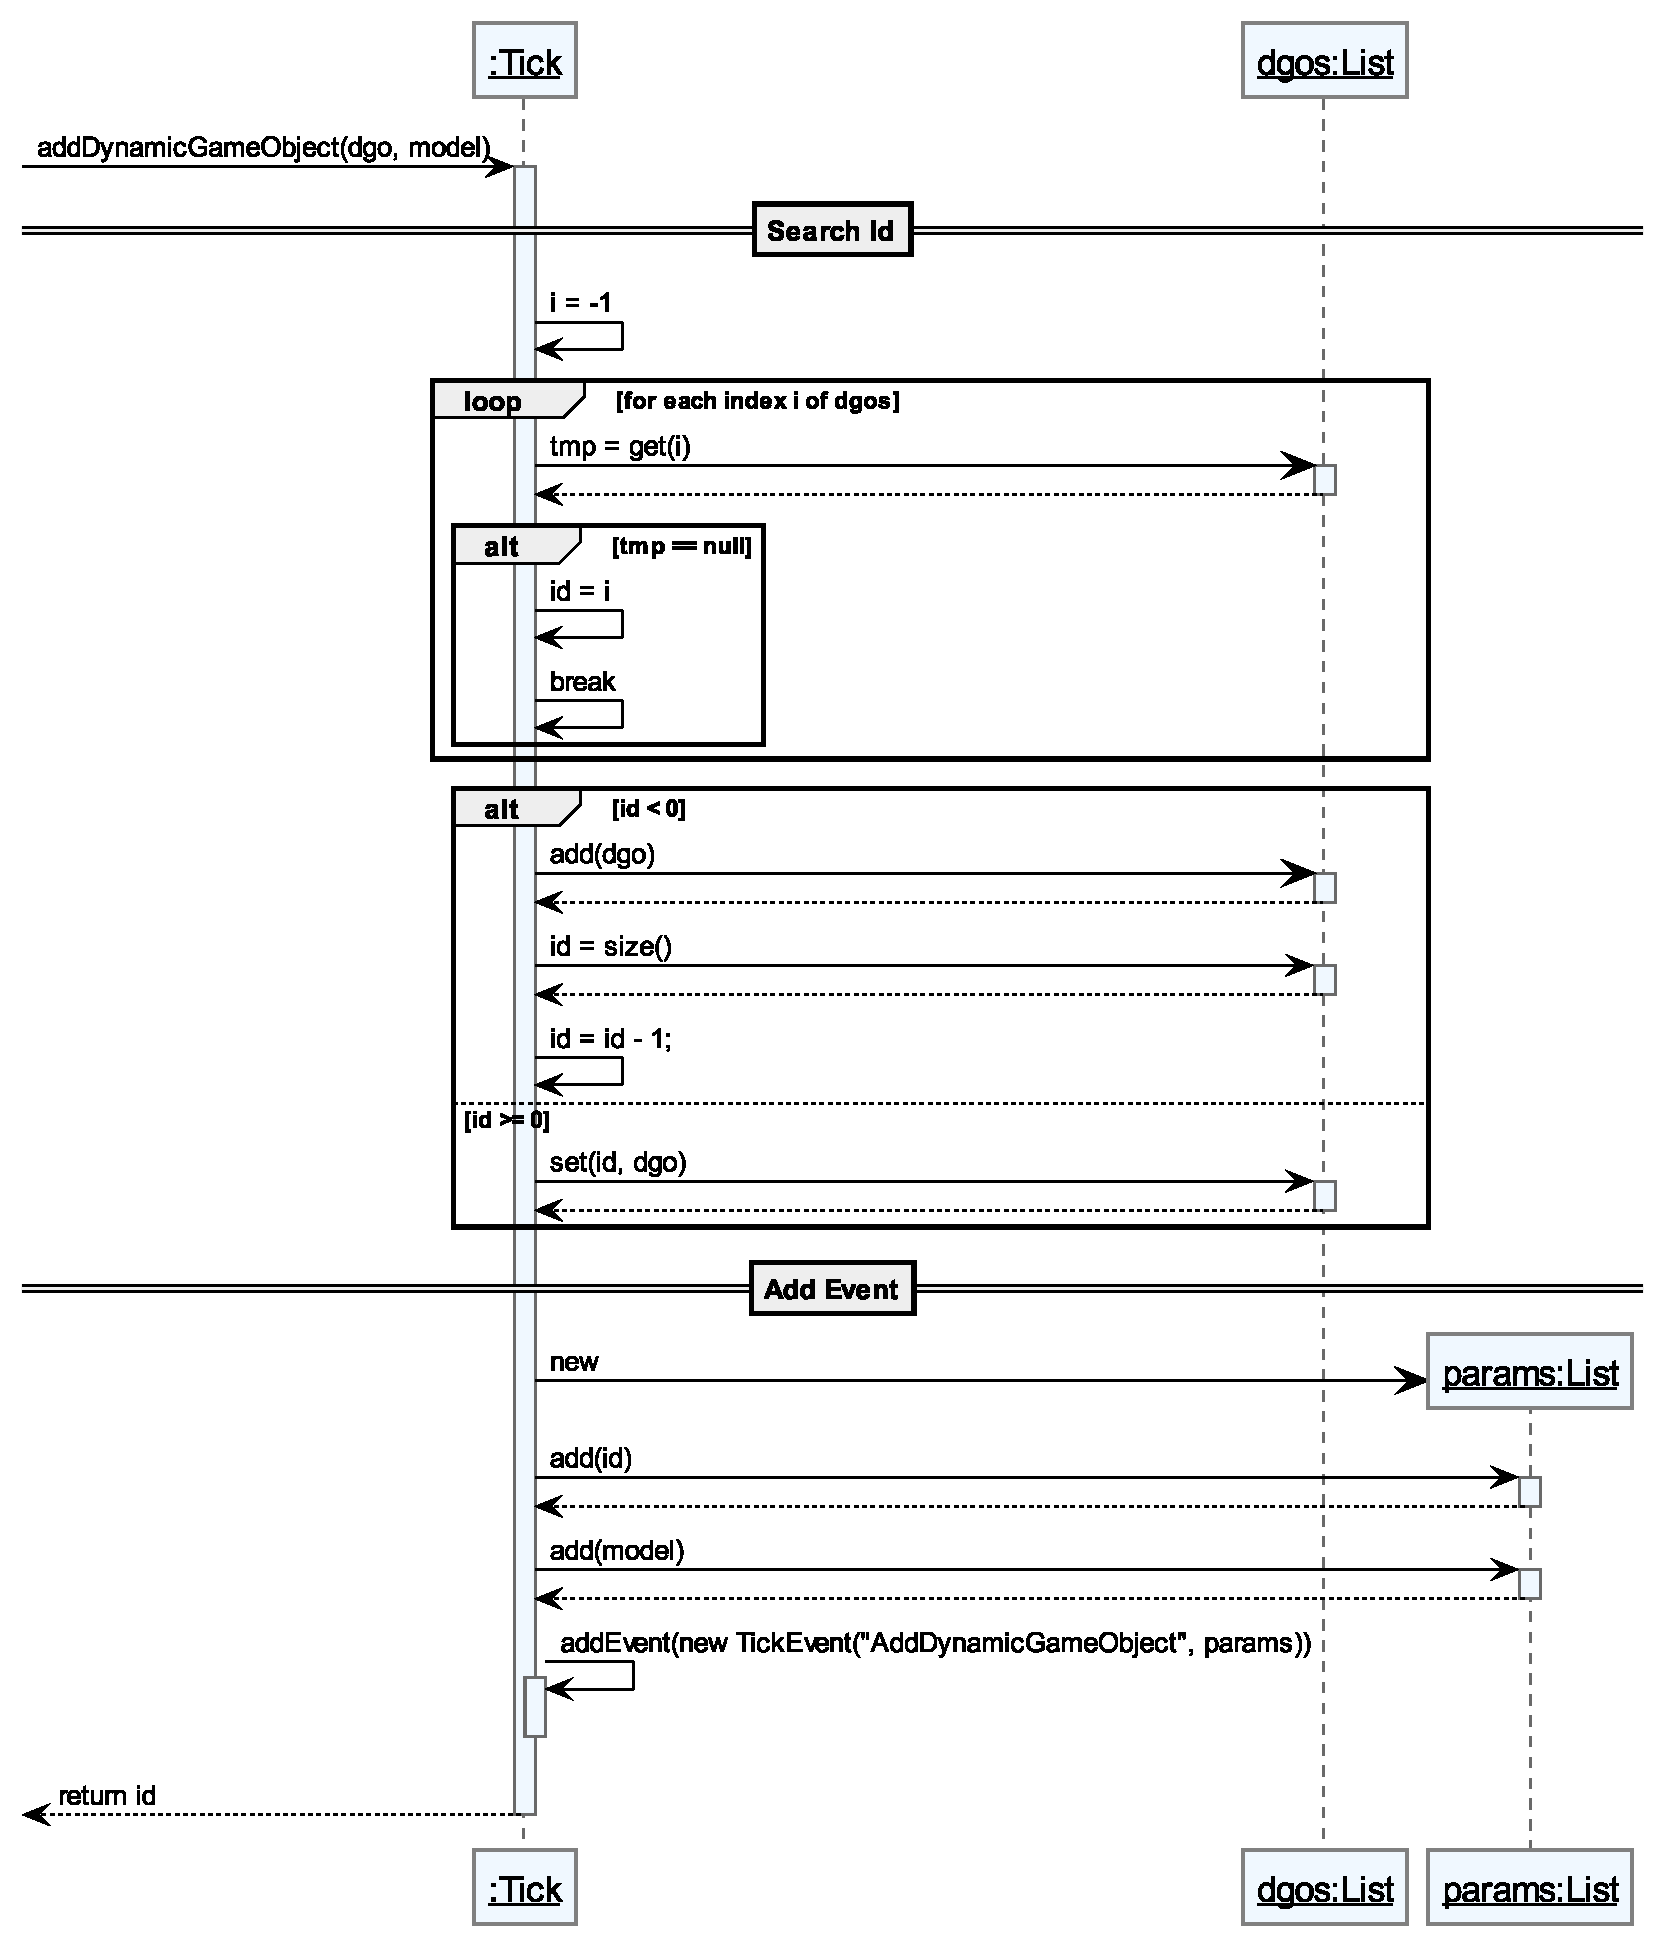
\includegraphics[width=\linewidth]{Interface/Tick_addBundle.eps}
    \captionof{figure}{Tick.addDynamicGameObject()}
\end{center}

\begin{center}
    \centering
    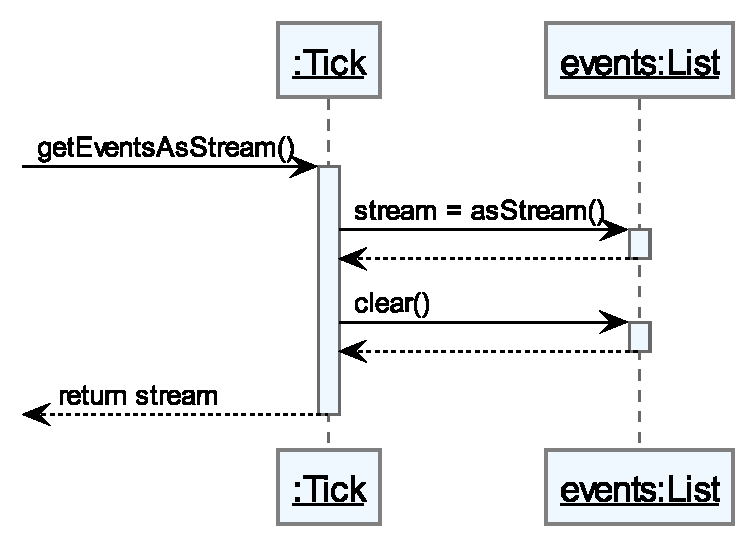
\includegraphics[width=0.5\linewidth]{Interface/Tick_getEventsAsStream.eps}
    \captionof{figure}{Tick.getEventsAsStream()}
\end{center}

\begin{center}
    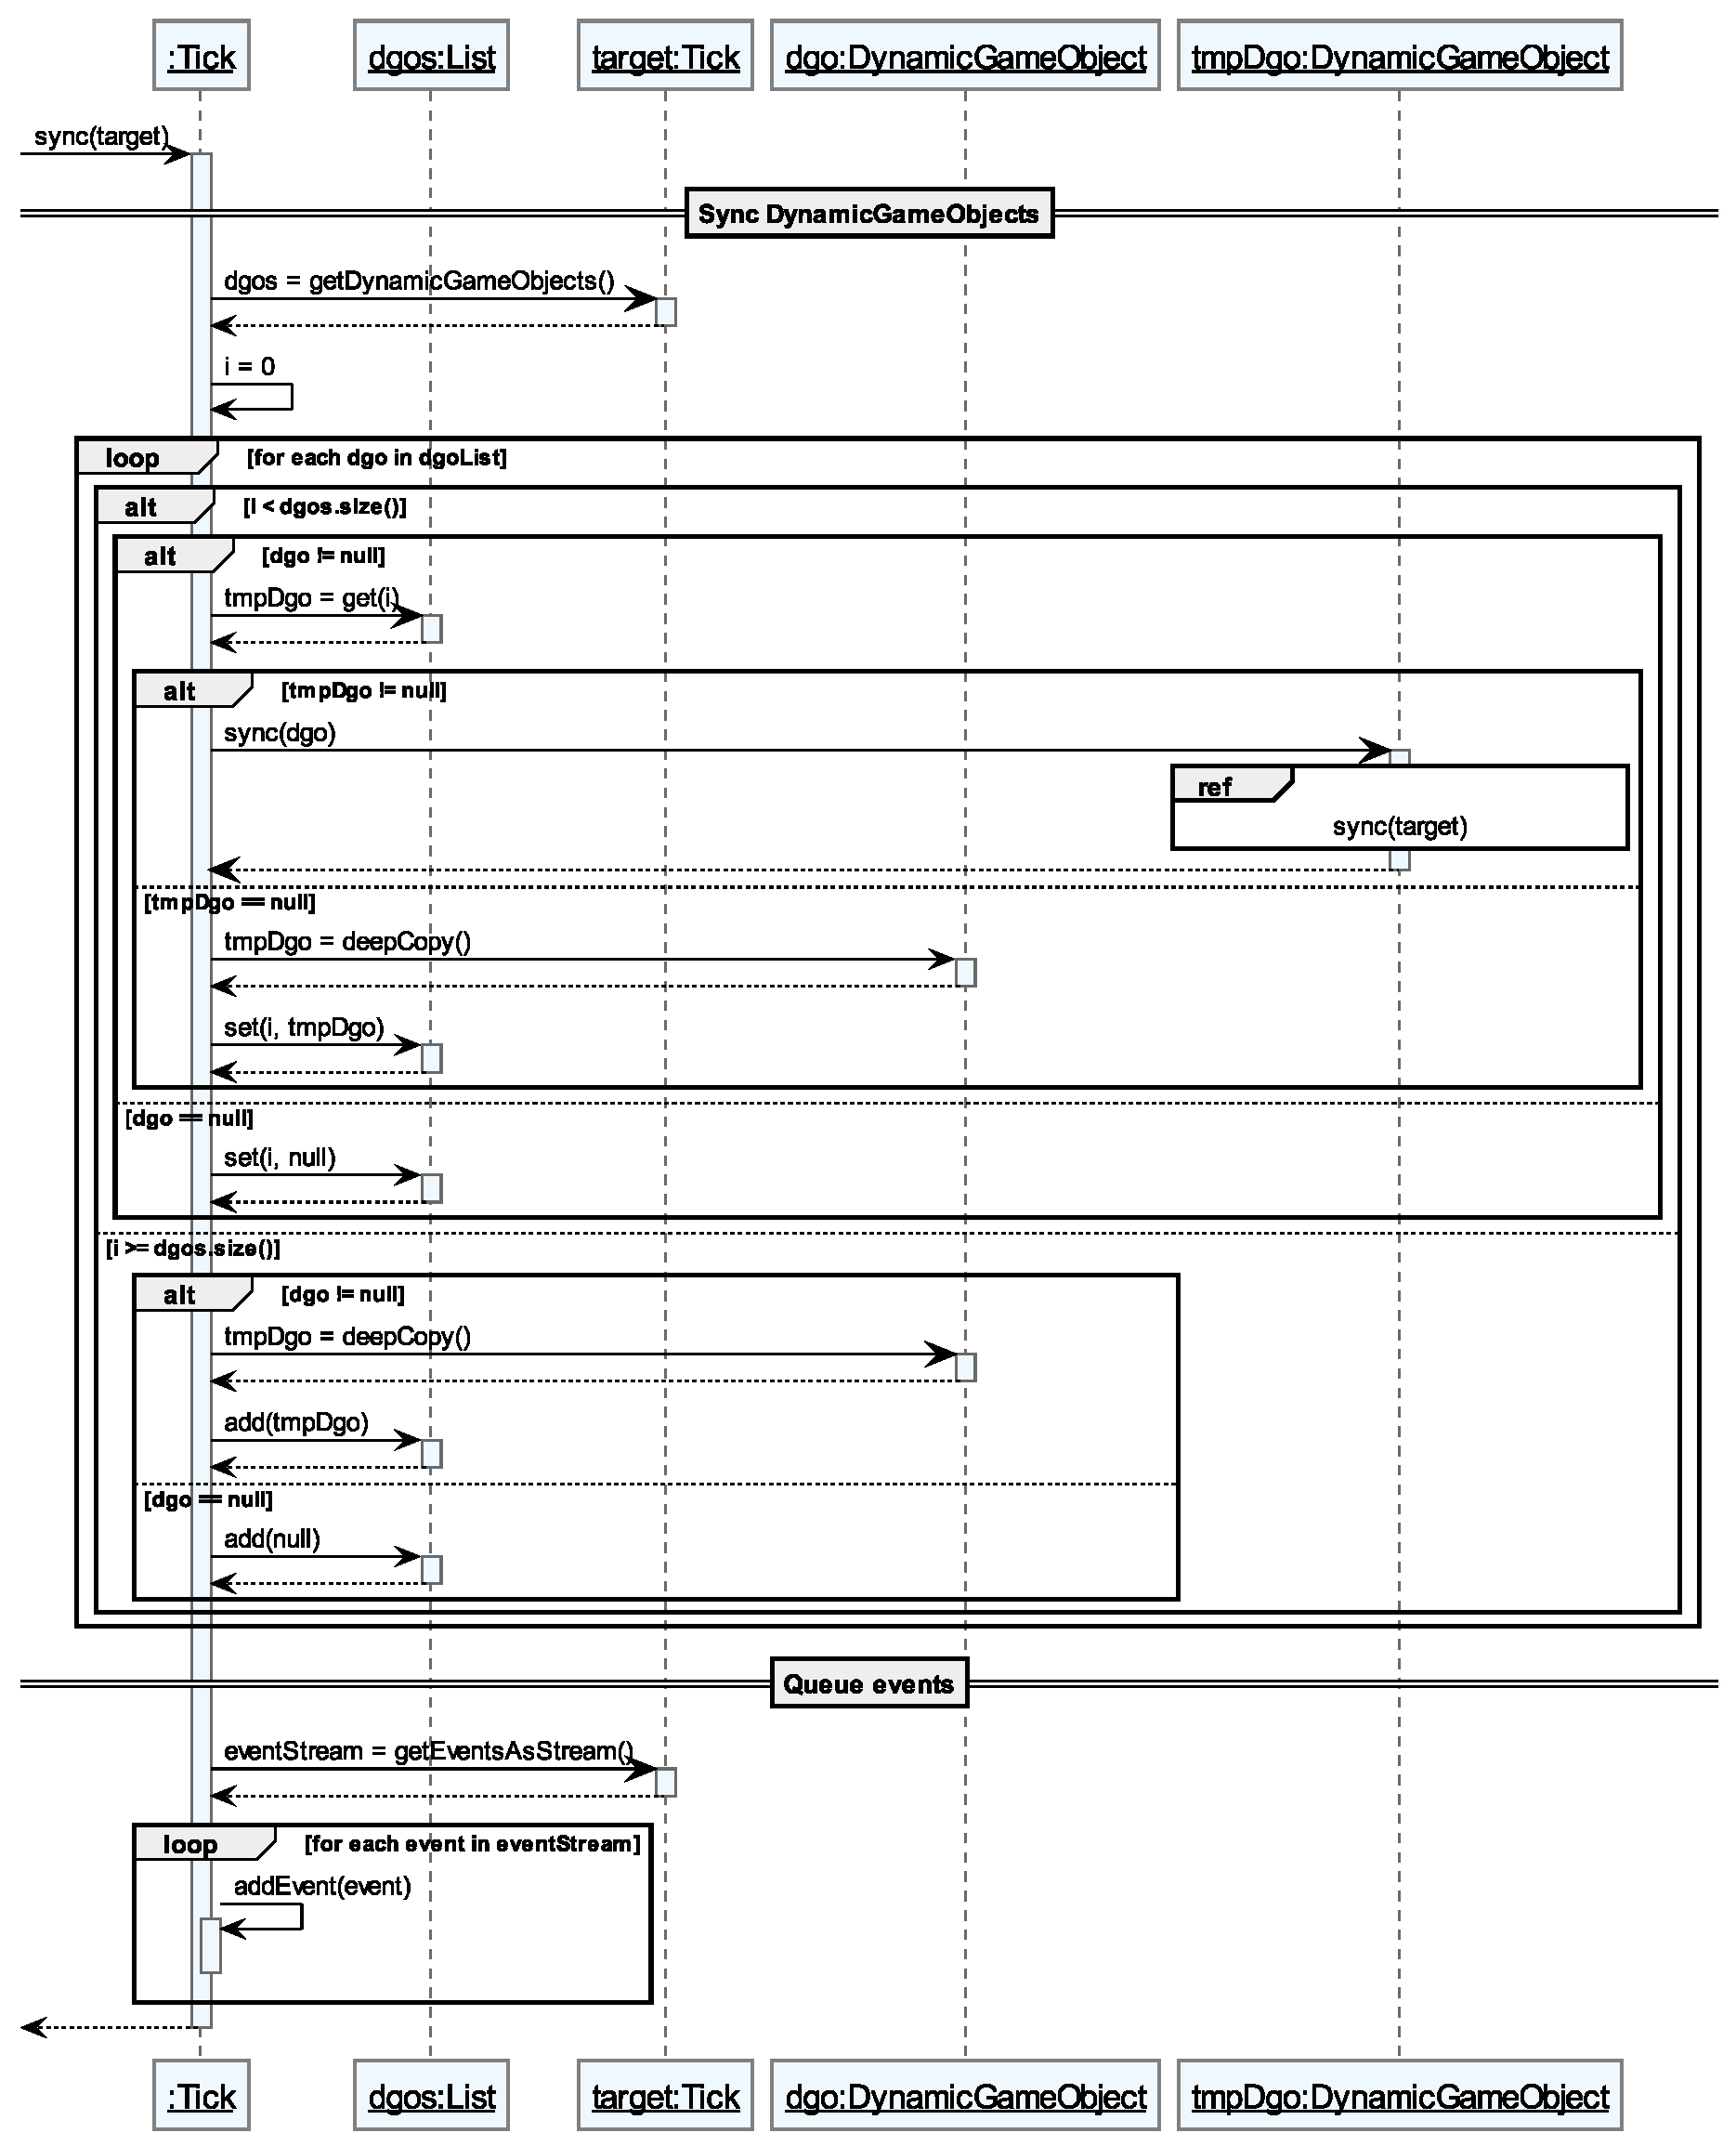
\includegraphics[width=\linewidth]{Interface/Tick_sync.eps}
    \captionof{figure}{Tick.sync()}
\end{center}

\subsubsection{tick.DynamicGameObject}
Die Funktionen sind analog zu den funktionen in \textit{tick.Tick}

\subsubsection{rendering.tick.TickProcessor}

\begin{center}
    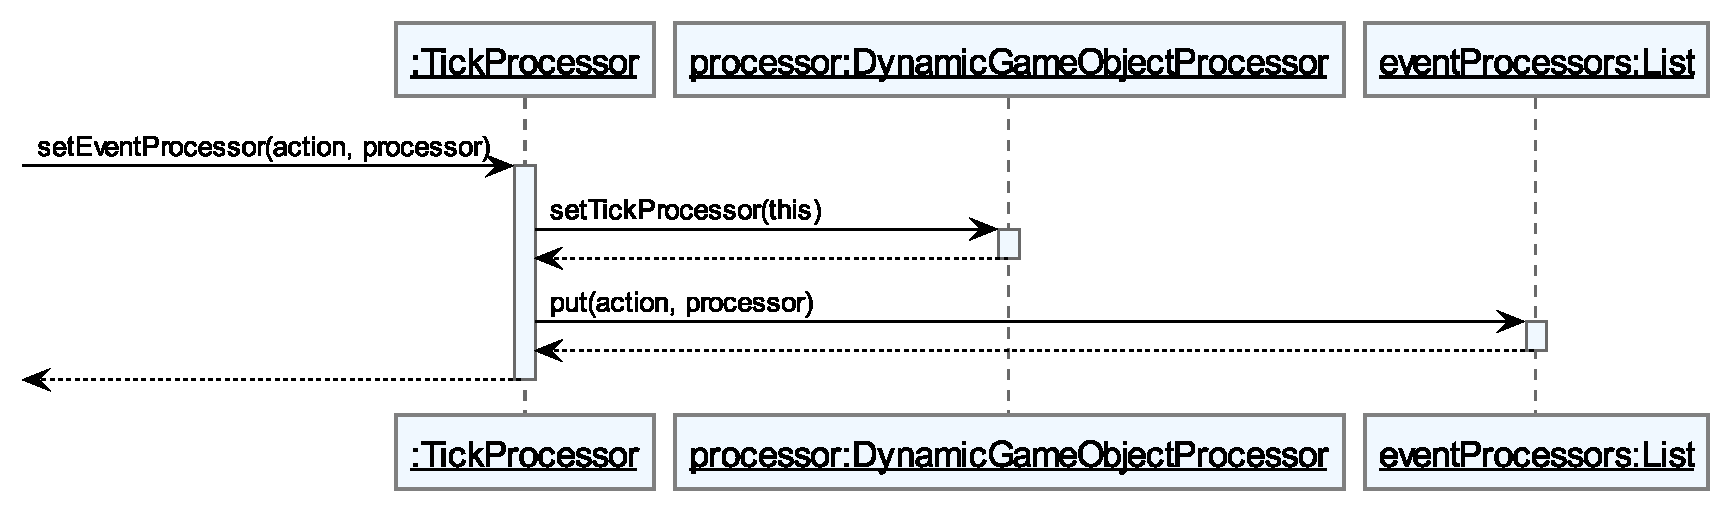
\includegraphics[width=\linewidth]{Interface/TickProcessor_setEventProcessor.eps}
    \captionof{figure}{TickProcessor.setEventProcessor()}
\end{center}

\begin{center}
    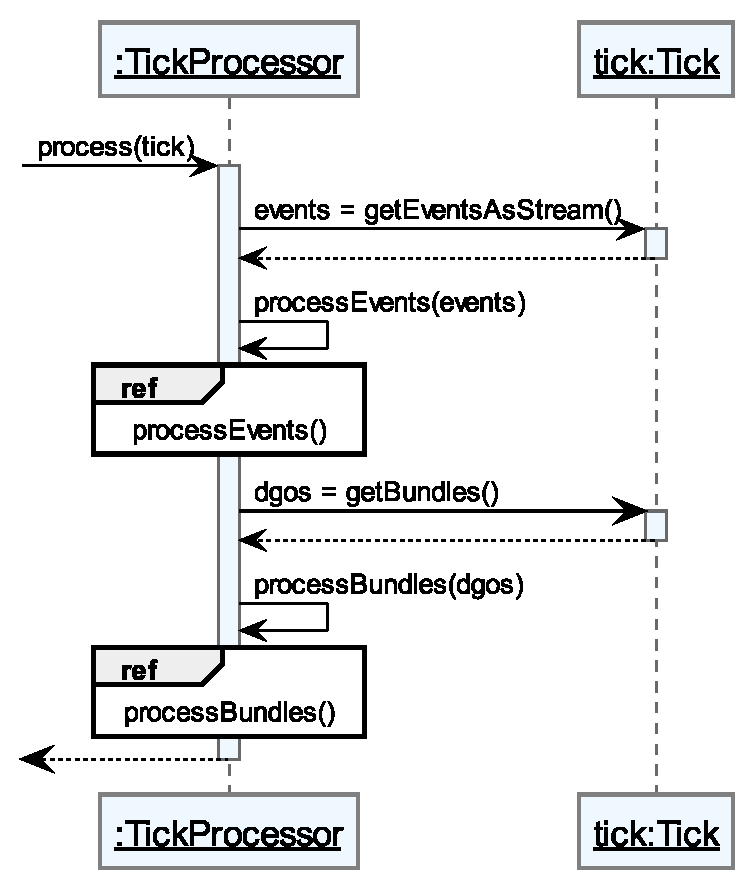
\includegraphics[width=0.5\linewidth]{Interface/TickProcessor_process.eps}
    \captionof{figure}{TickProcessor.process()}
\end{center}

\begin{center}
    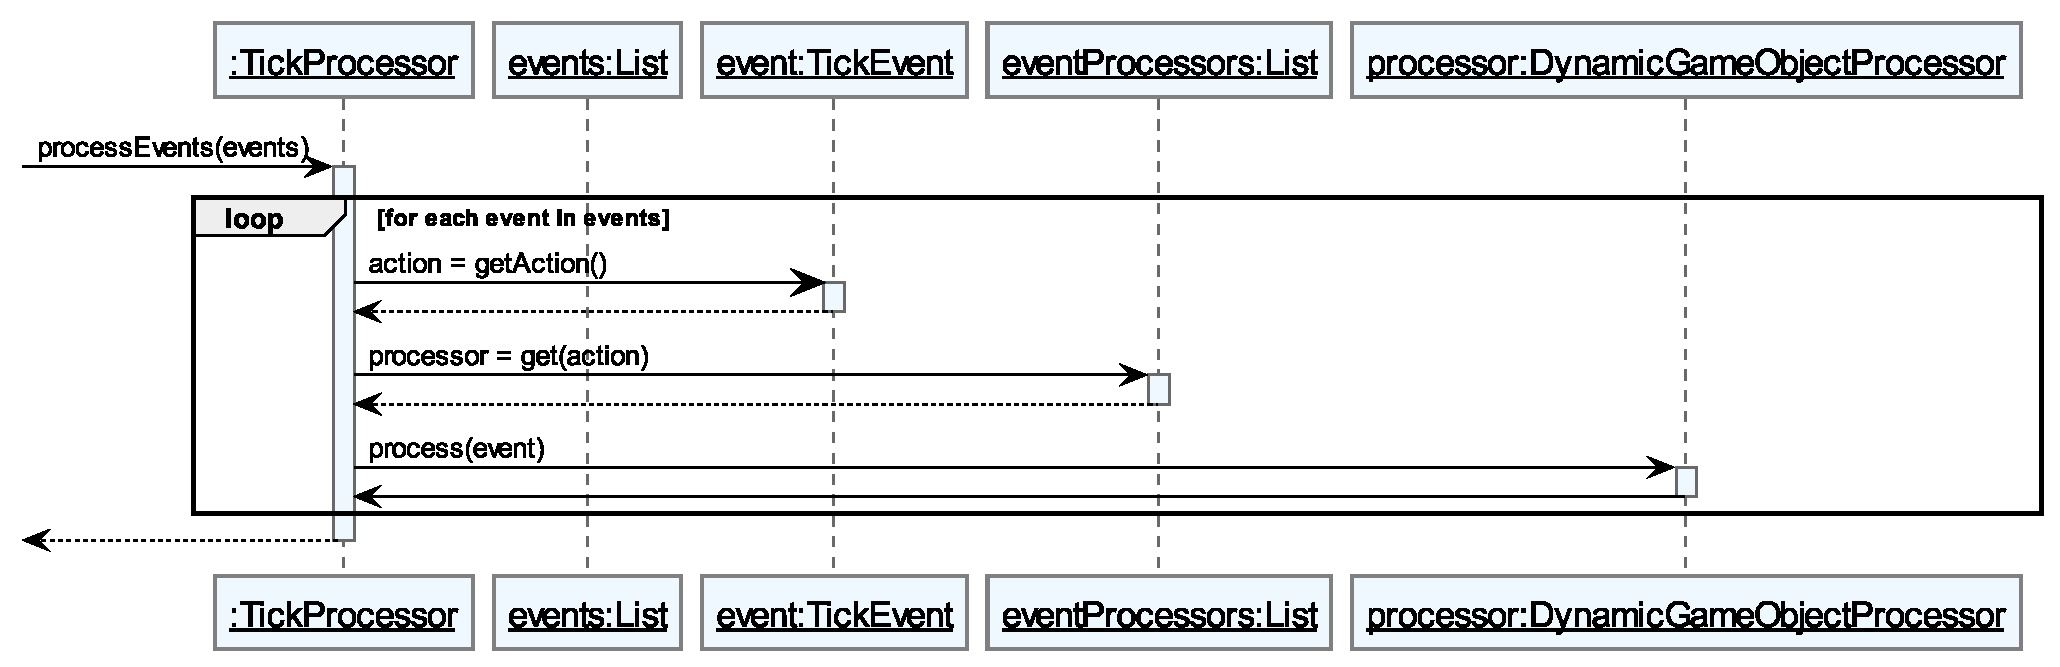
\includegraphics[width=\linewidth]{Interface/TickProcessor_processEvents.eps}
    \captionof{figure}{TickProcessor.processEvents()}
\end{center}

\begin{center}
    \centering
    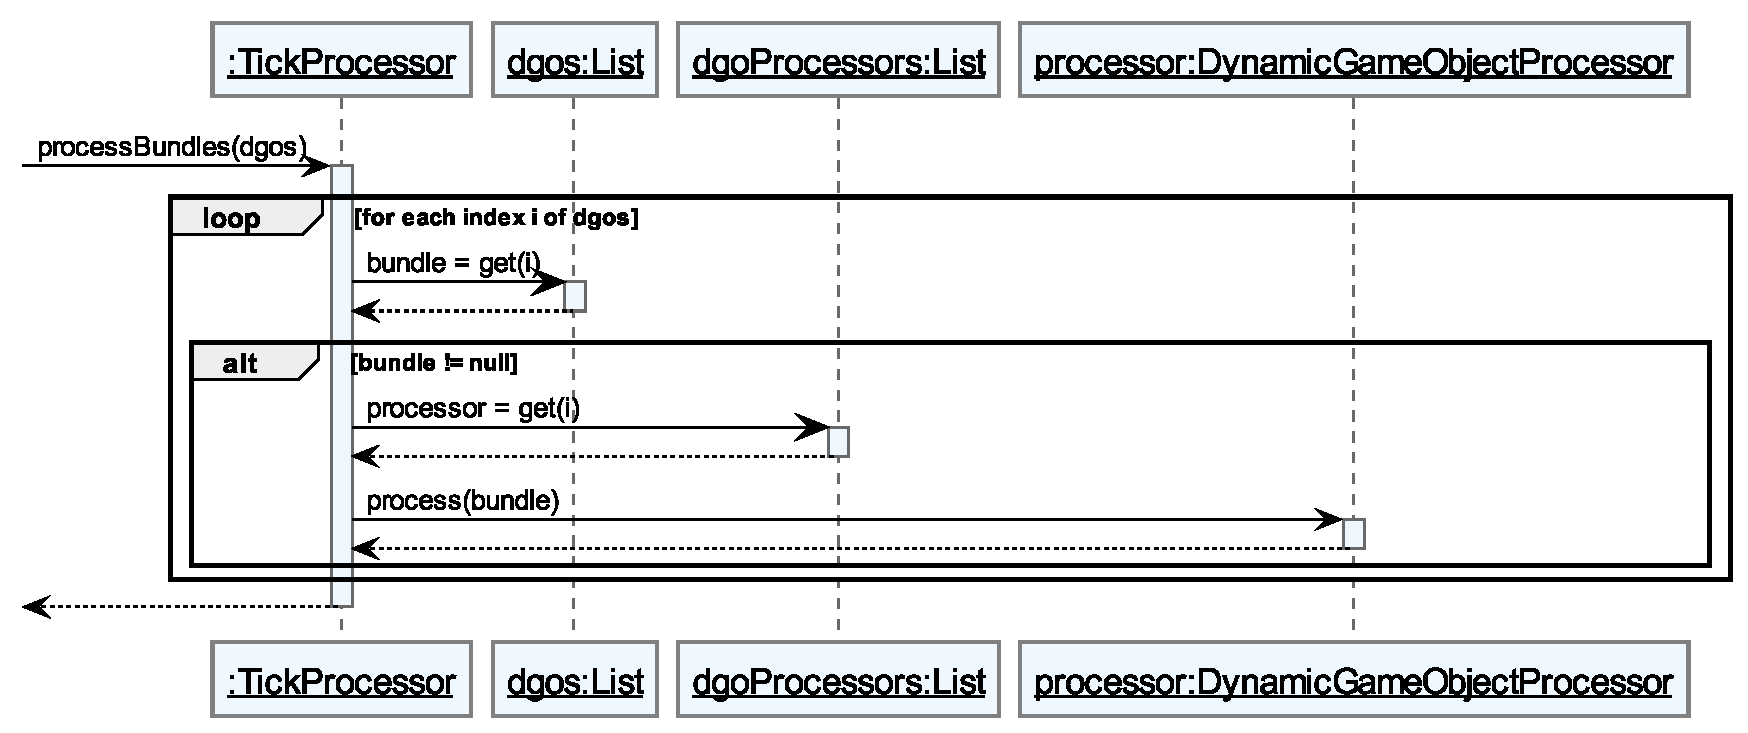
\includegraphics[width=\linewidth]{Interface/TickProcessor_processBundles.eps}
    \captionof{figure}{TickProcessor.processDynamicGameObjects()}
\end{center}

\subsubsection{rendering.tick.DynamicGameObjectProcessor}
Die Funktionen sind analog zu den funktionen in \textit{rendering.tick.TickProcessor}
		\pagebreak
		\subsection{Assets}

\subsubsection{assets.JsonModelProvider}
\begin{center}
    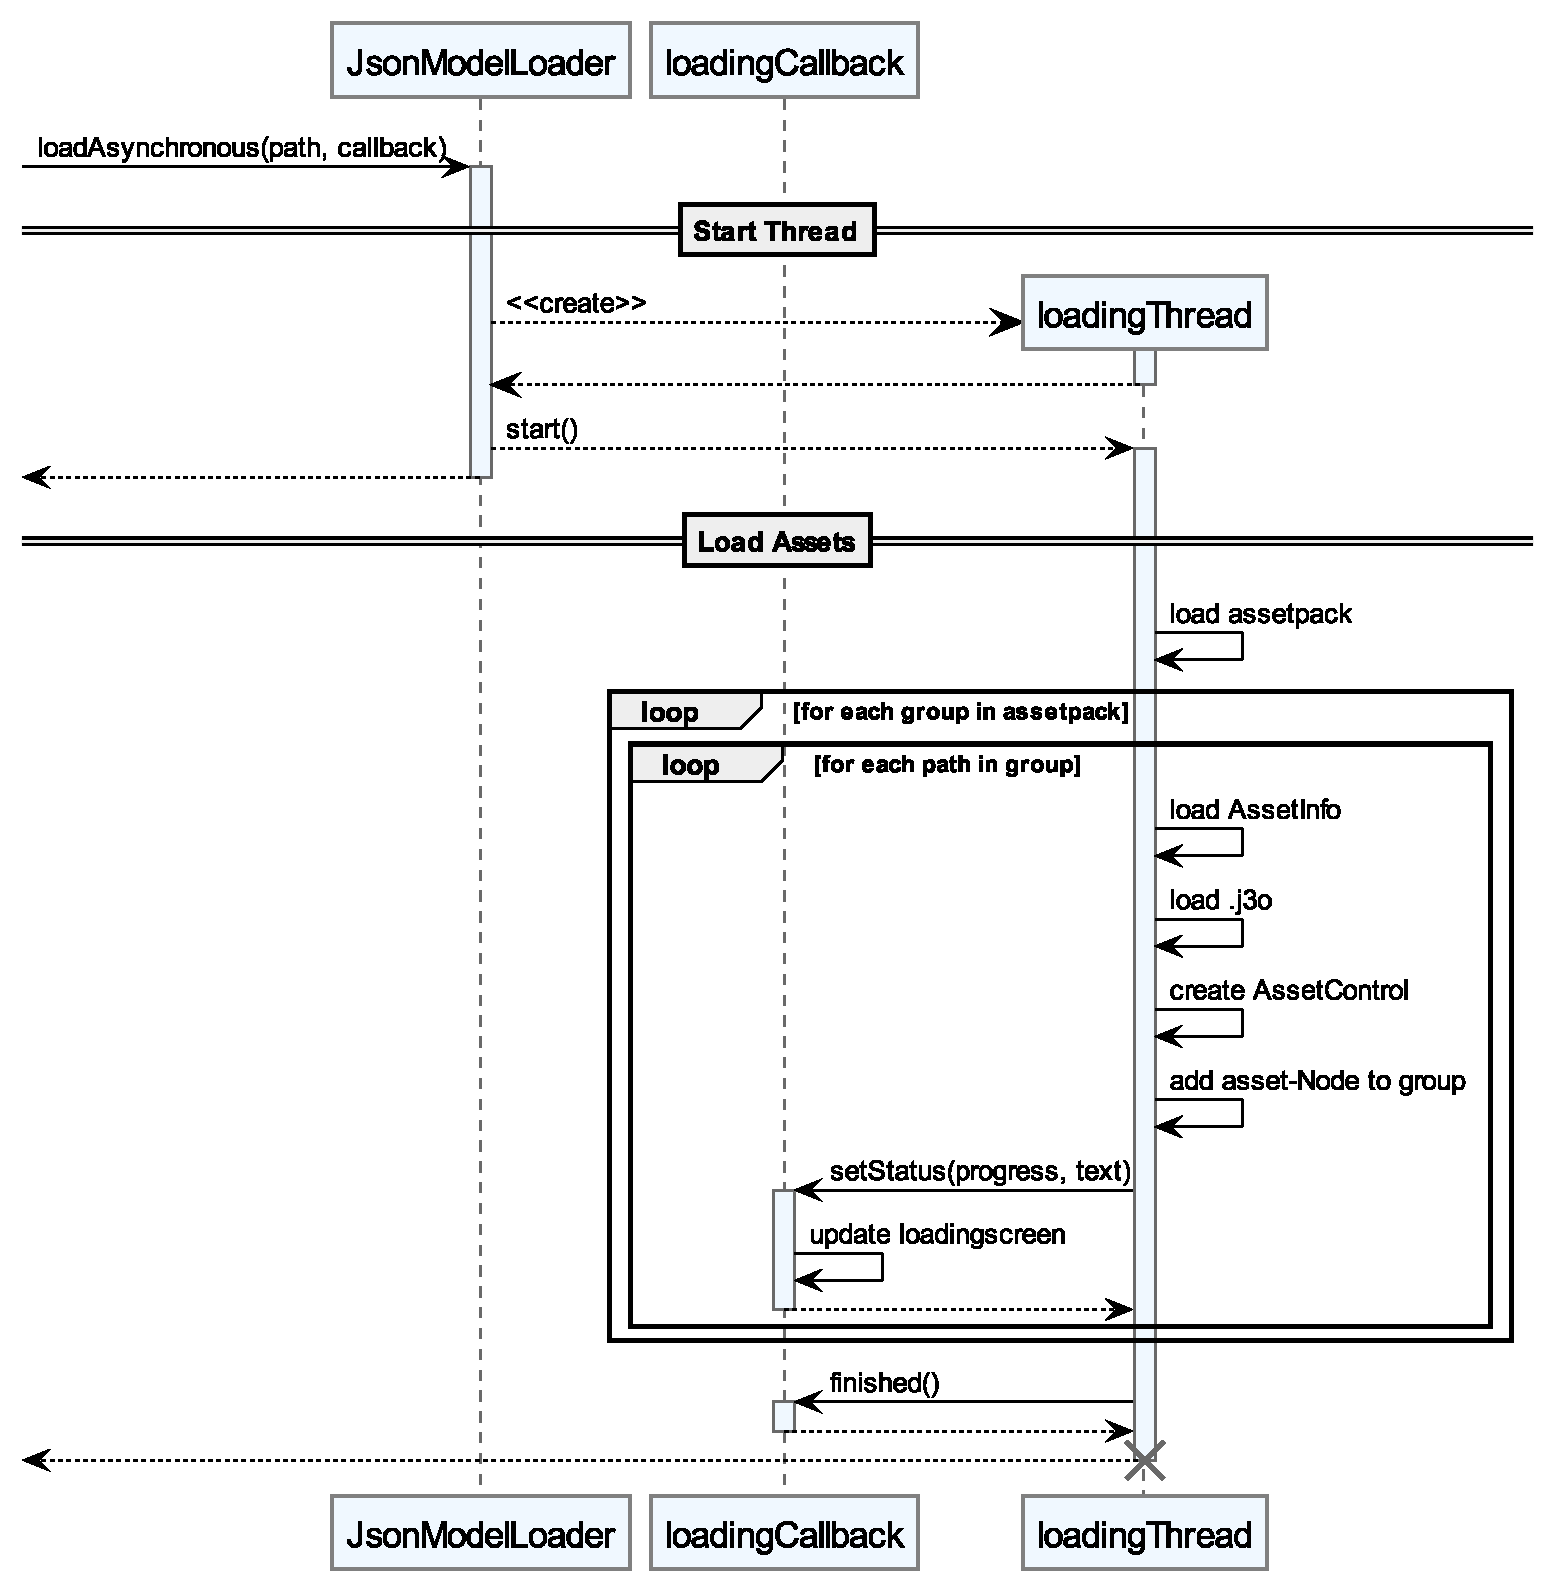
\includegraphics[width=\linewidth]{Assets/Assets_loadAsynchronous.eps}
    \captionof{figure}{JsonModelProvider.loadAsynchronous()}
\end{center}
		\pagebreak
		\subsection{Generierung}

\begin{figure} [htbp]
    \centering
    \centering
    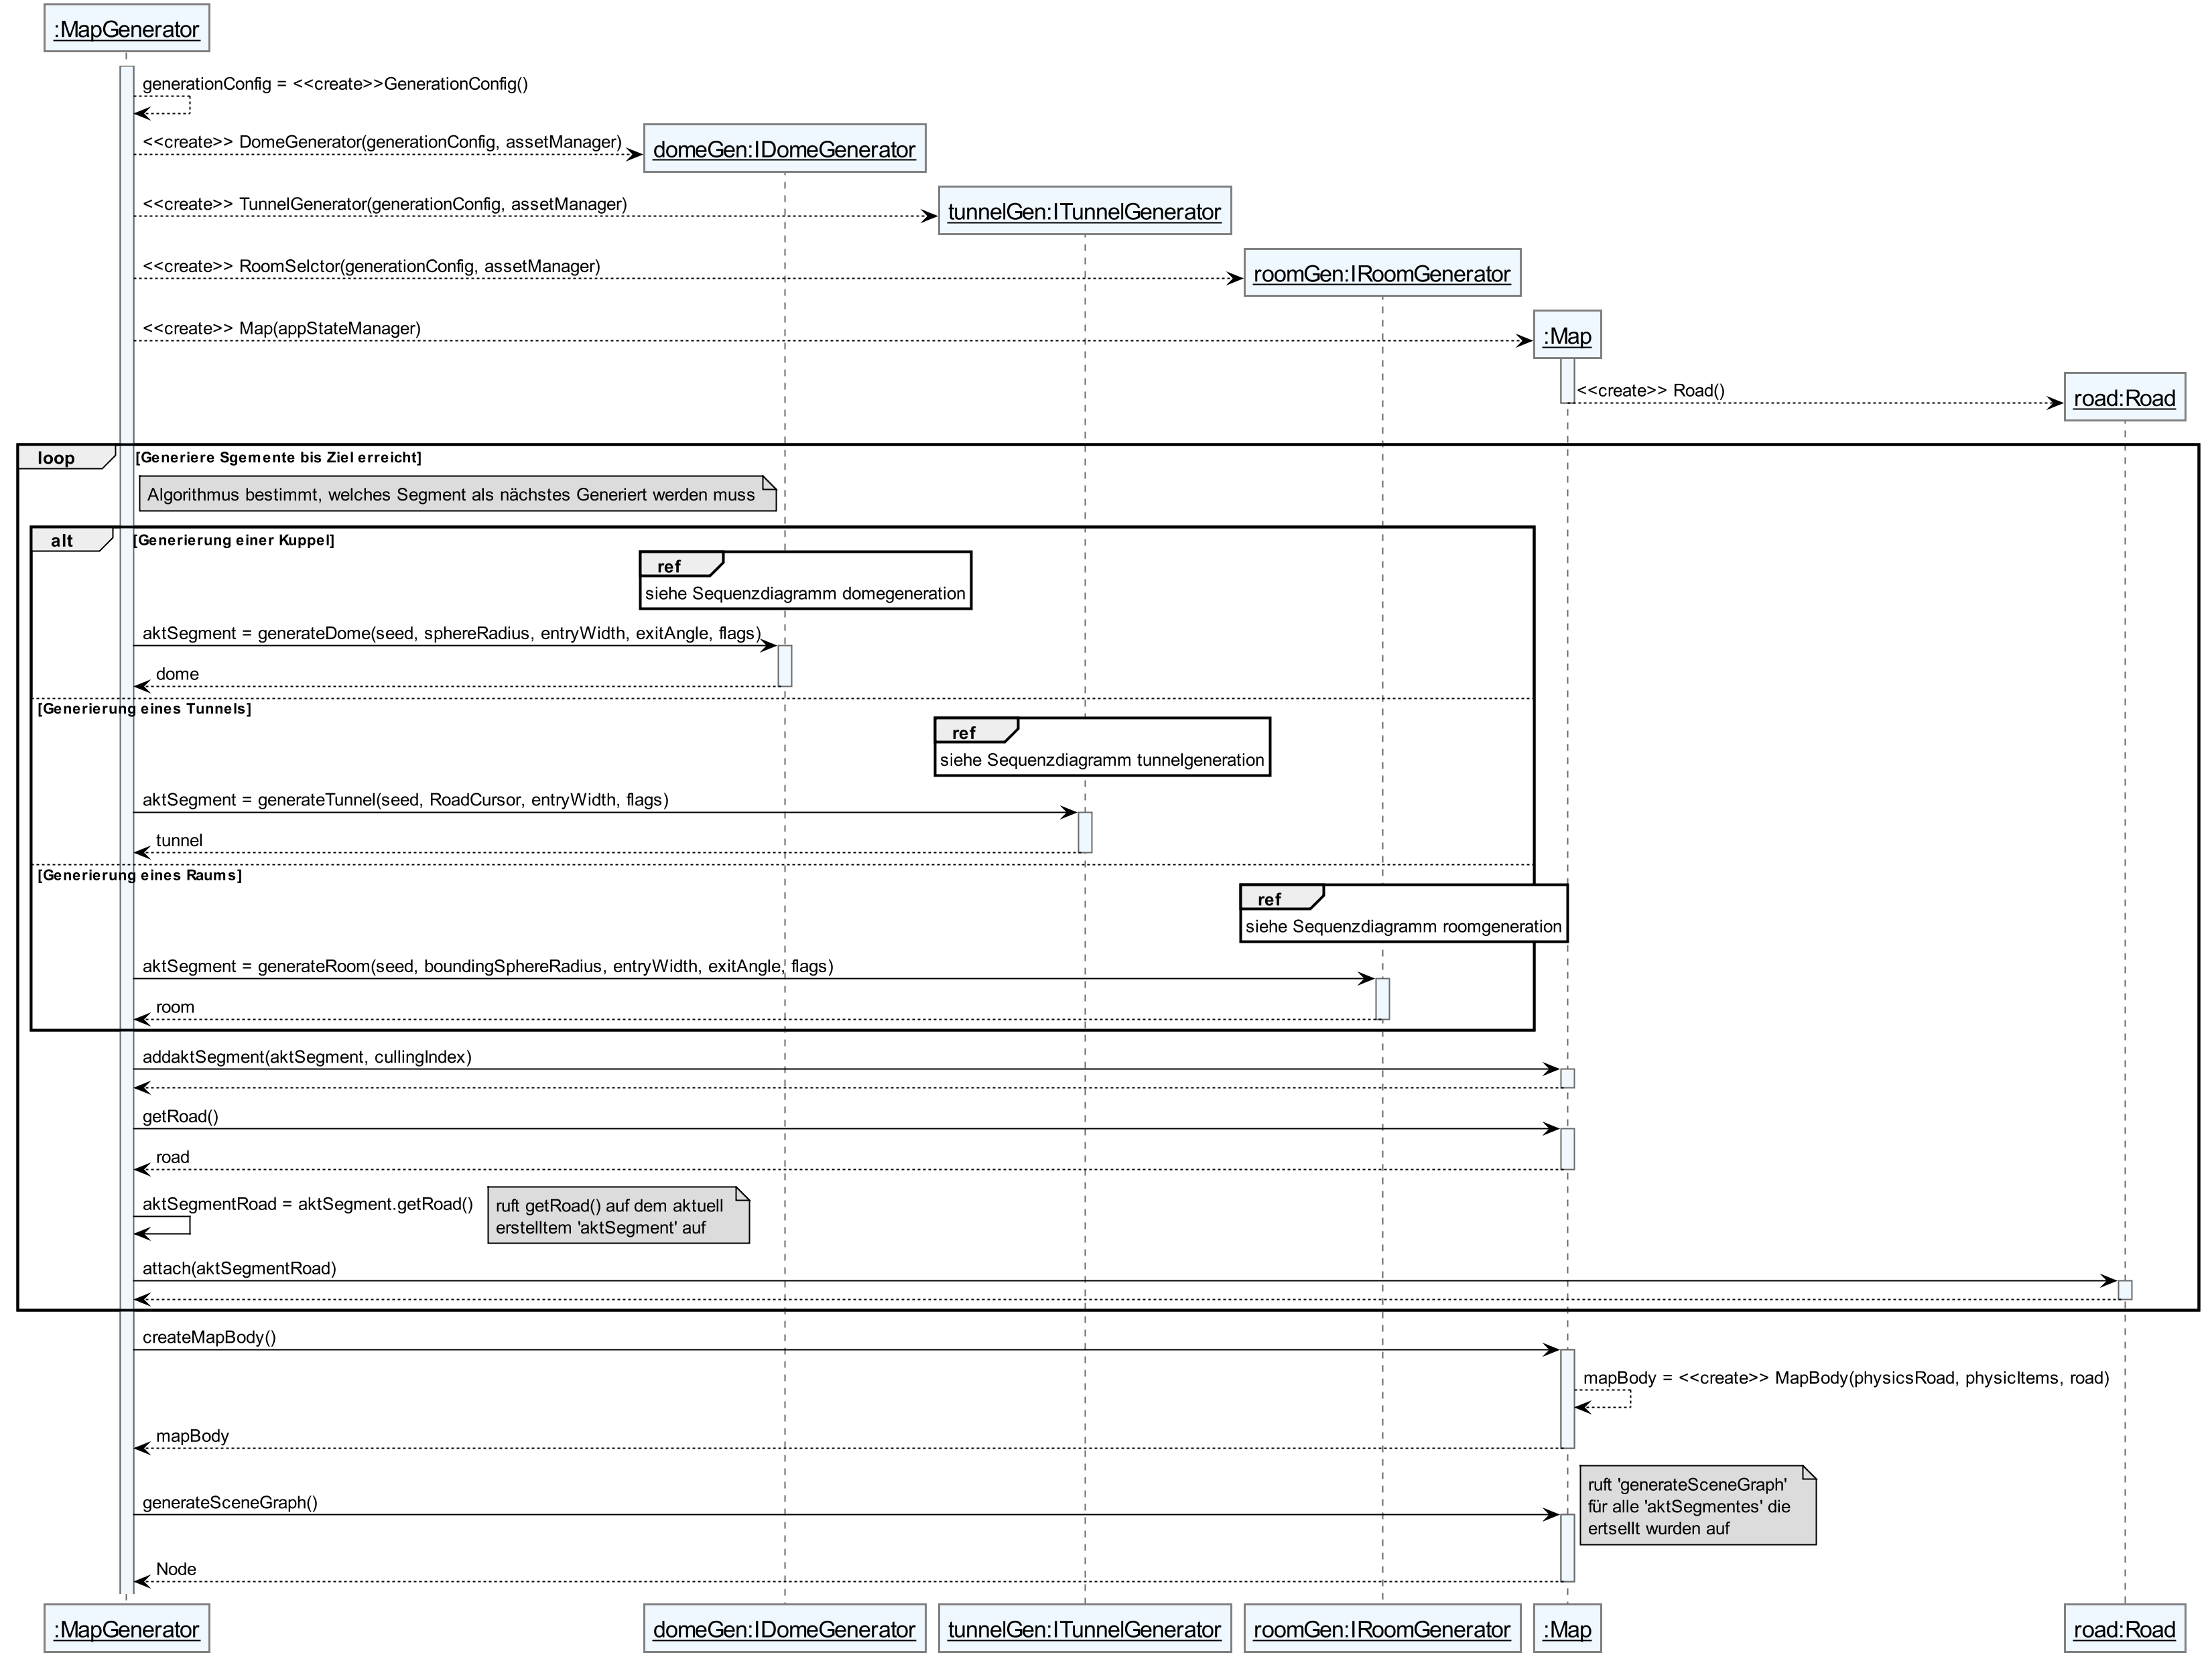
\includegraphics[width=\linewidth]{./Generierung/Bilder/mapgenerationSequenz.png}
    \caption{Sequenzdiagramm mapgeneration}
\end{figure}

\begin{figure} [htbp]
    \centering
    \centering
    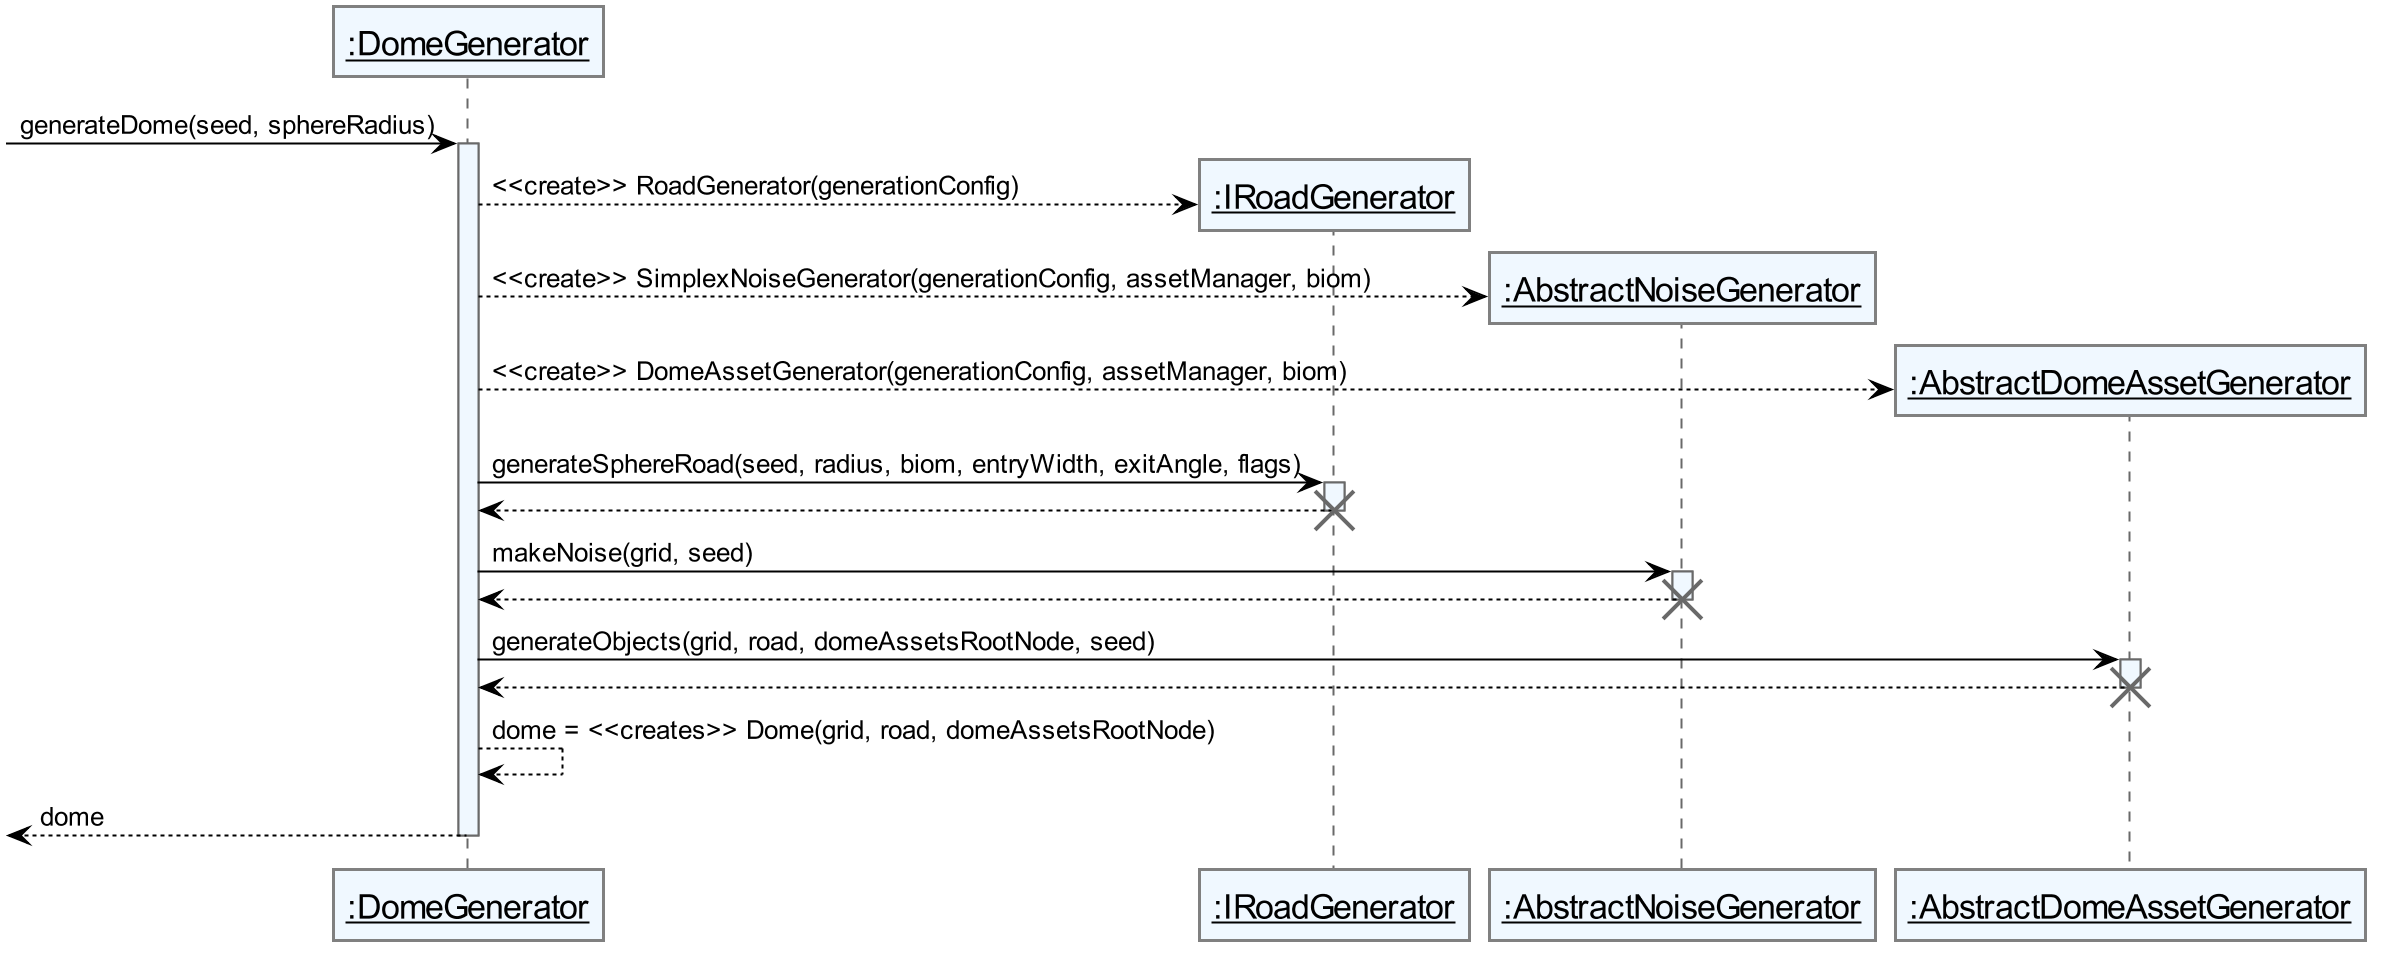
\includegraphics[width=\linewidth]{./Generierung/Bilder/domeGenerationSequenz.png}
    \caption{Sequenzdiagramm domegeneration}
\end{figure}

\begin{figure} [htbp]
    \centering
    \centering
    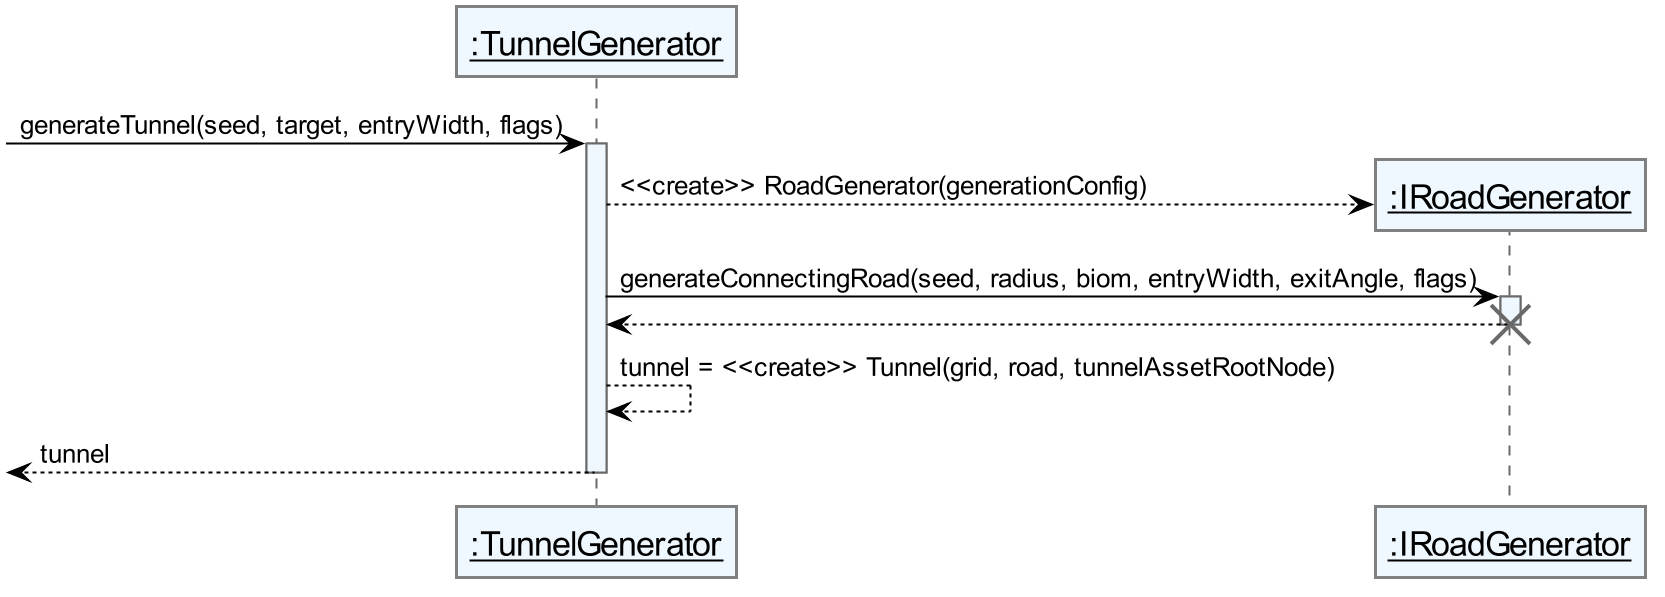
\includegraphics[width=\linewidth]{./Generierung/Bilder/tunnelGenerationSequenz.png}
    \caption{Sequenzdiagramm tunnelgeneration}
\end{figure}

\begin{figure} [htbp]
    \centering
    \centering
    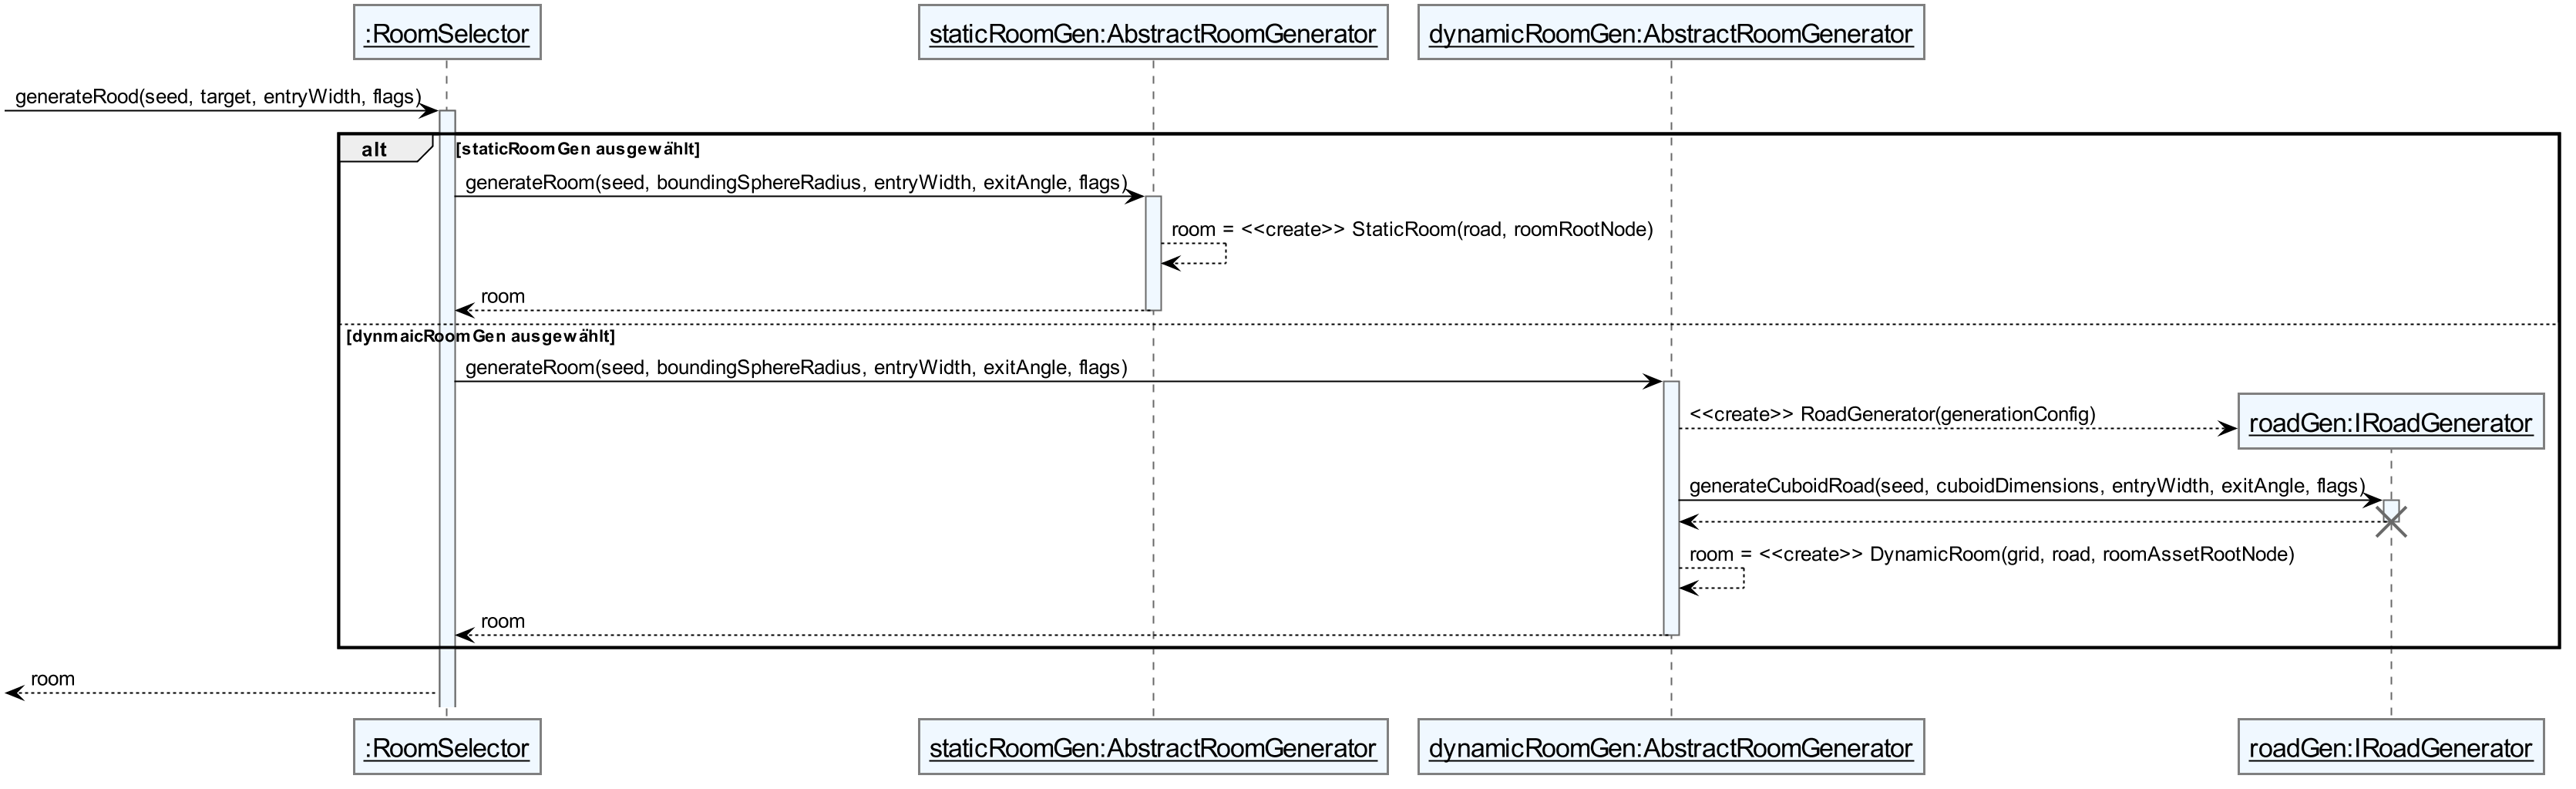
\includegraphics[width=\linewidth]{./Generierung/Bilder/roomGenerationSequenz.png}
    \caption{Sequenzdiagramm roomgeneration}
\end{figure}


		\pagebreak
		\subsection{GUI}

\begin{center}

    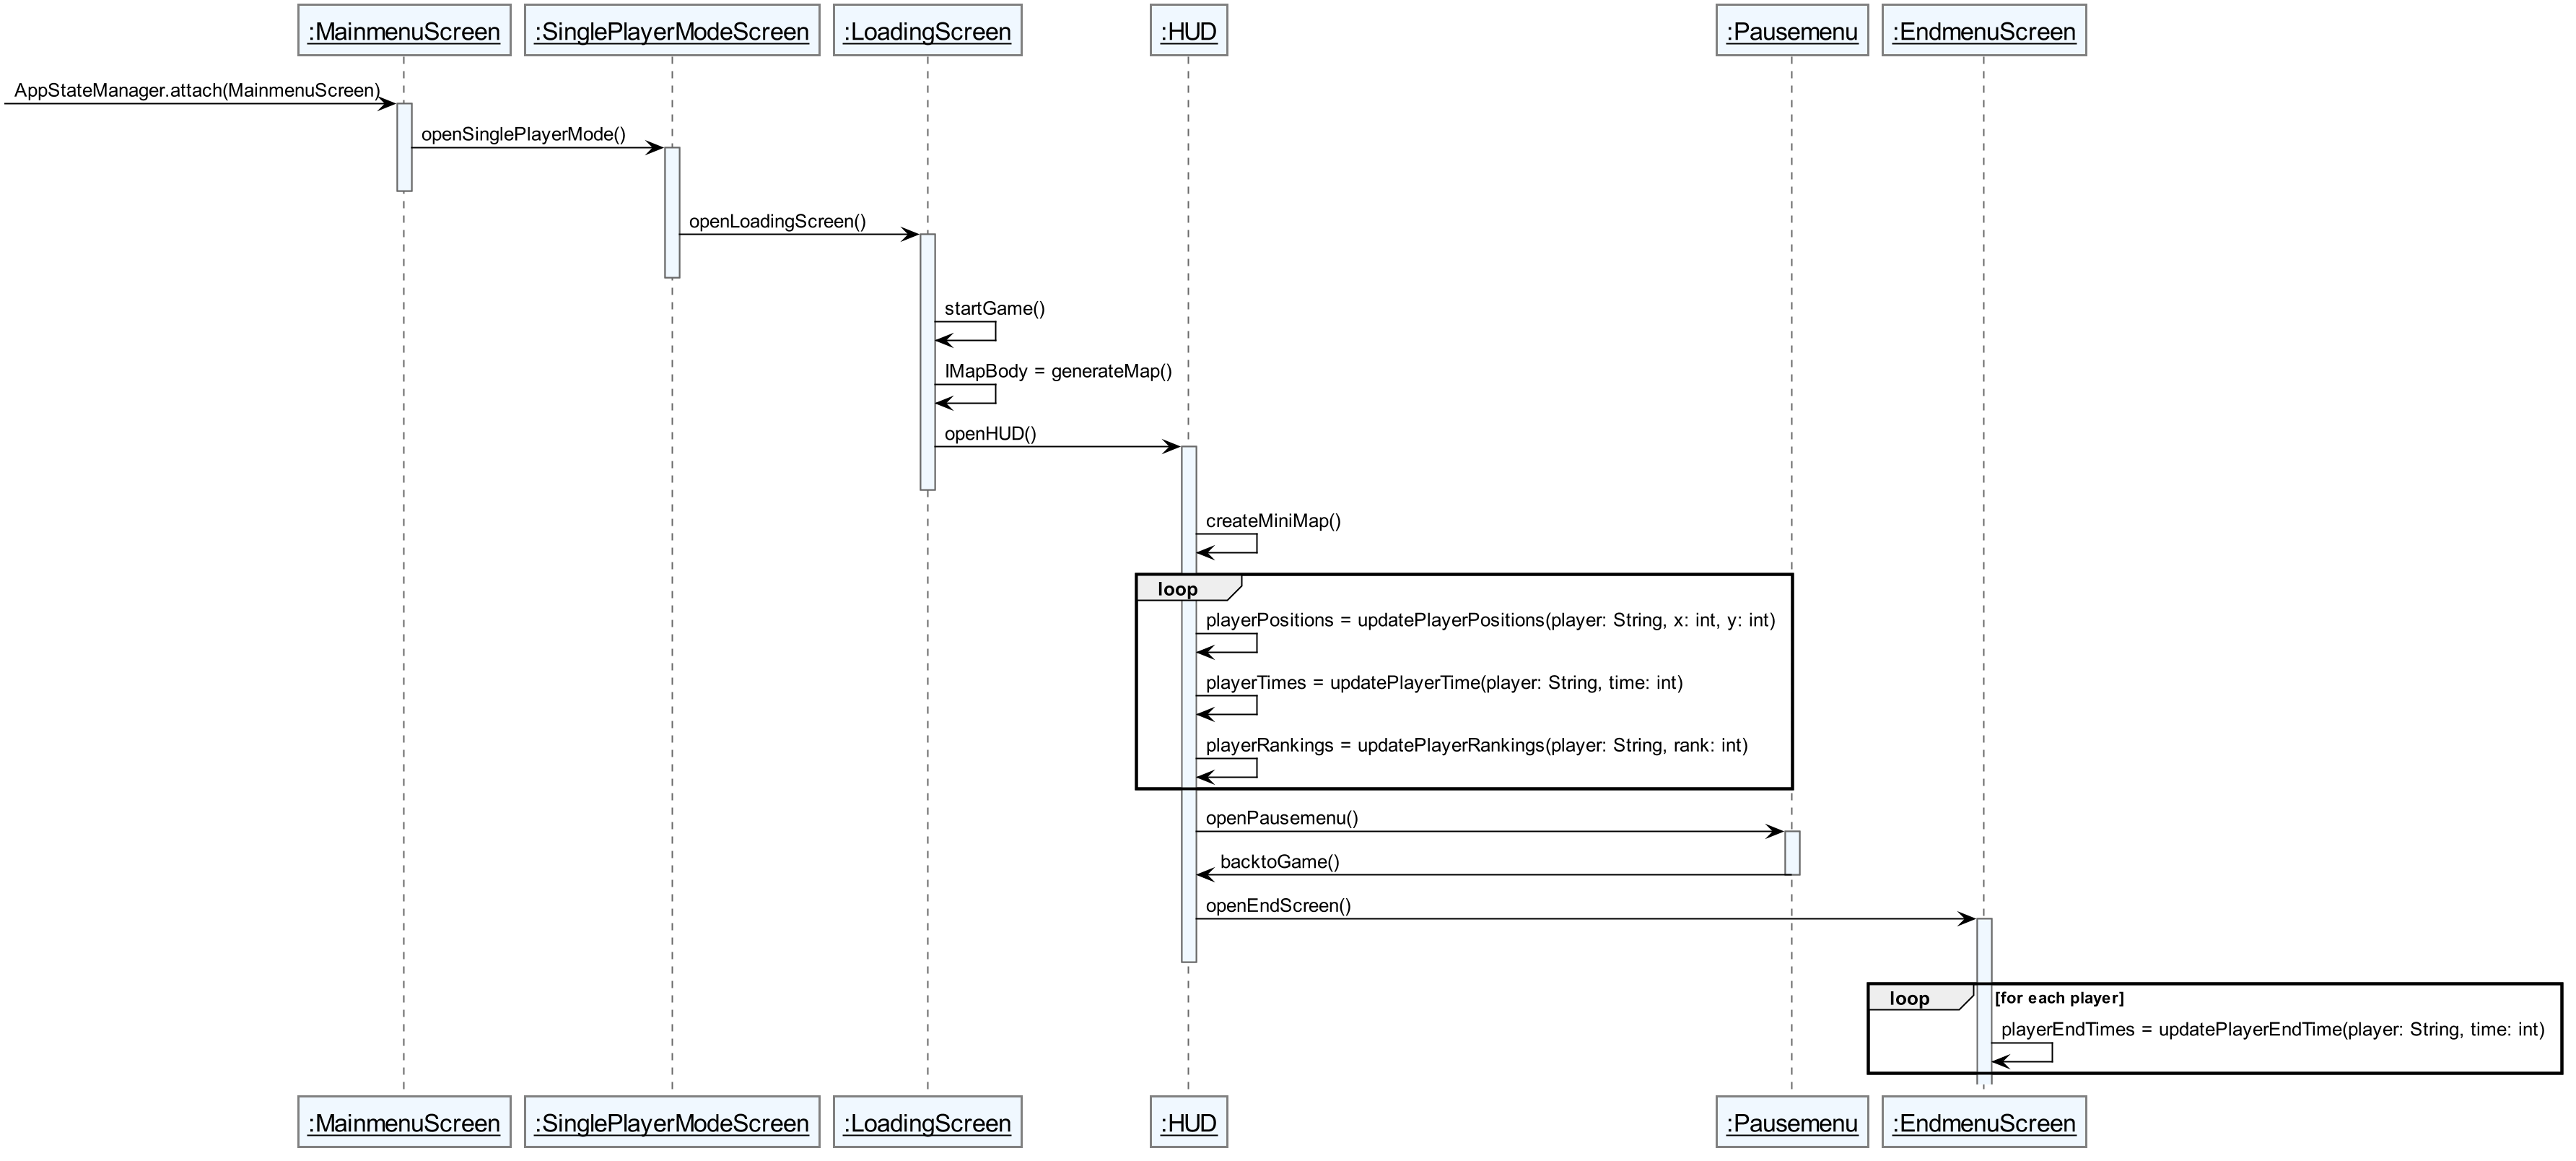
\includegraphics[width=\linewidth]{./GUI/GUI_Bilder/AllScreens.png}
    \captionof{figure}{Alle Menü-Bildschirme besuchen}
    \label{fig:AllScreens}

    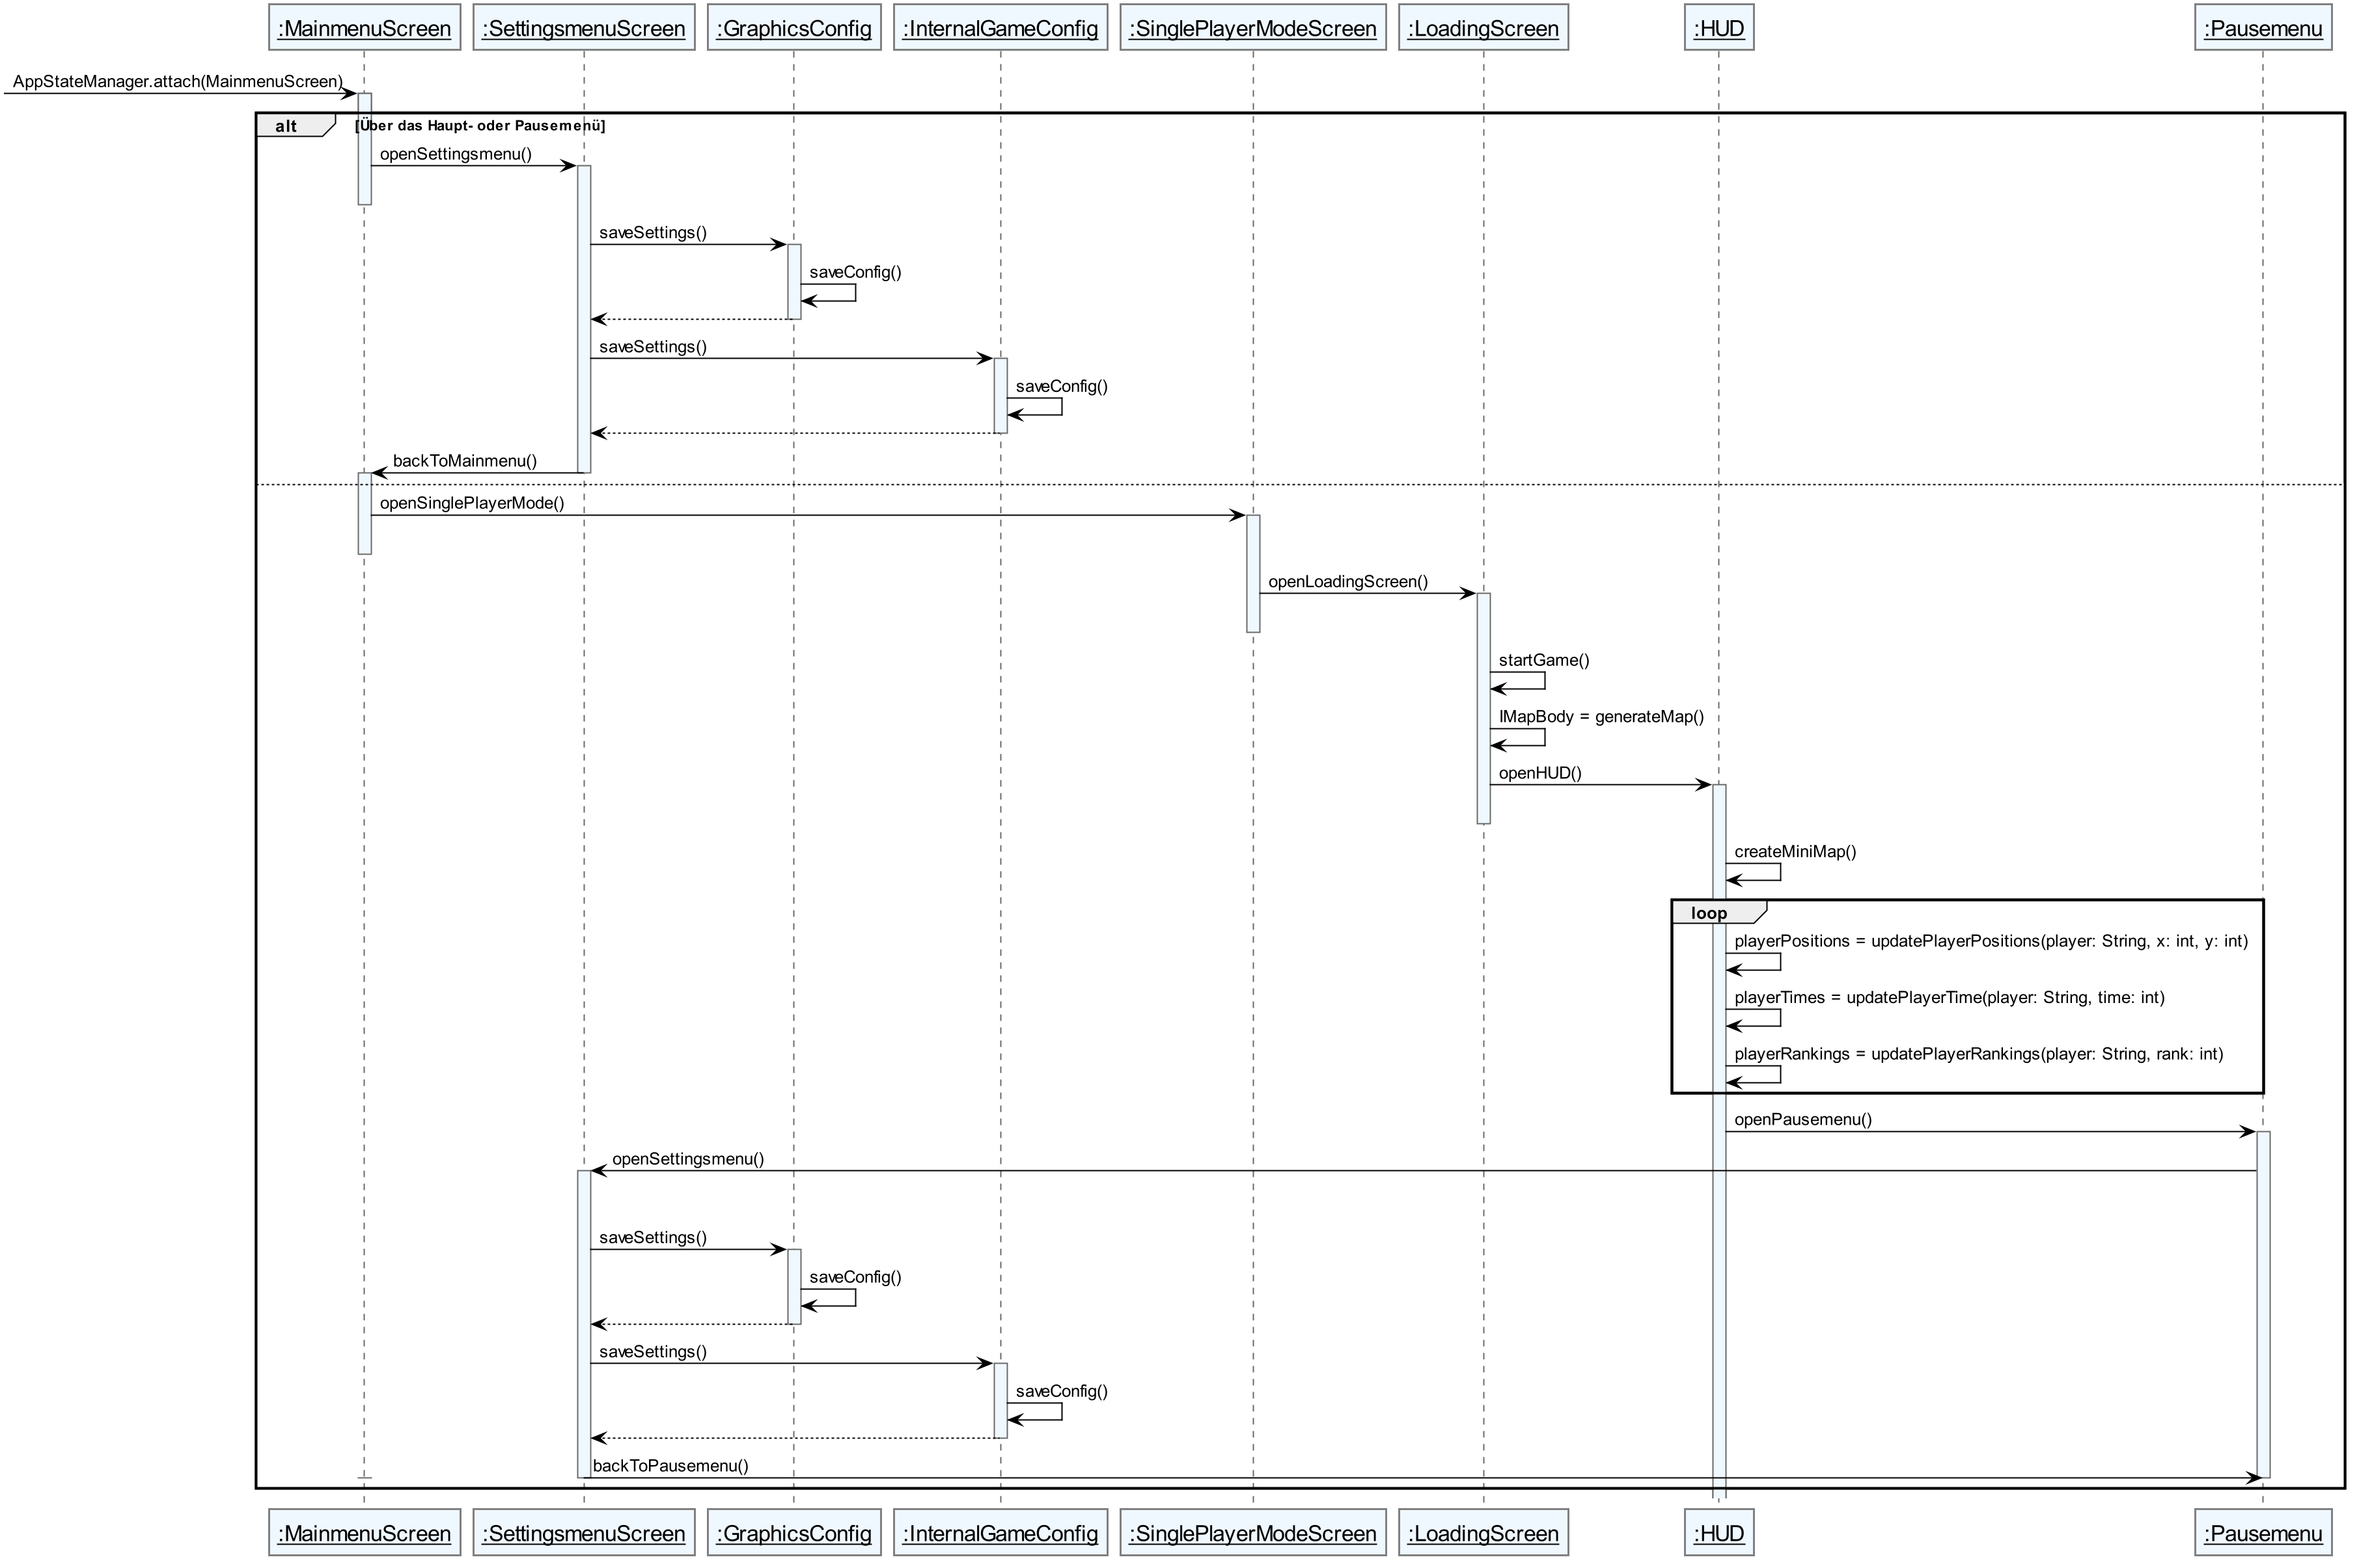
\includegraphics[width=\linewidth]{./GUI/GUI_Bilder/EditSettings.png}
    \captionof{figure}{Menü-Einstellungen bearbeiten und speichern}
    \label{fig:EditSettings}

    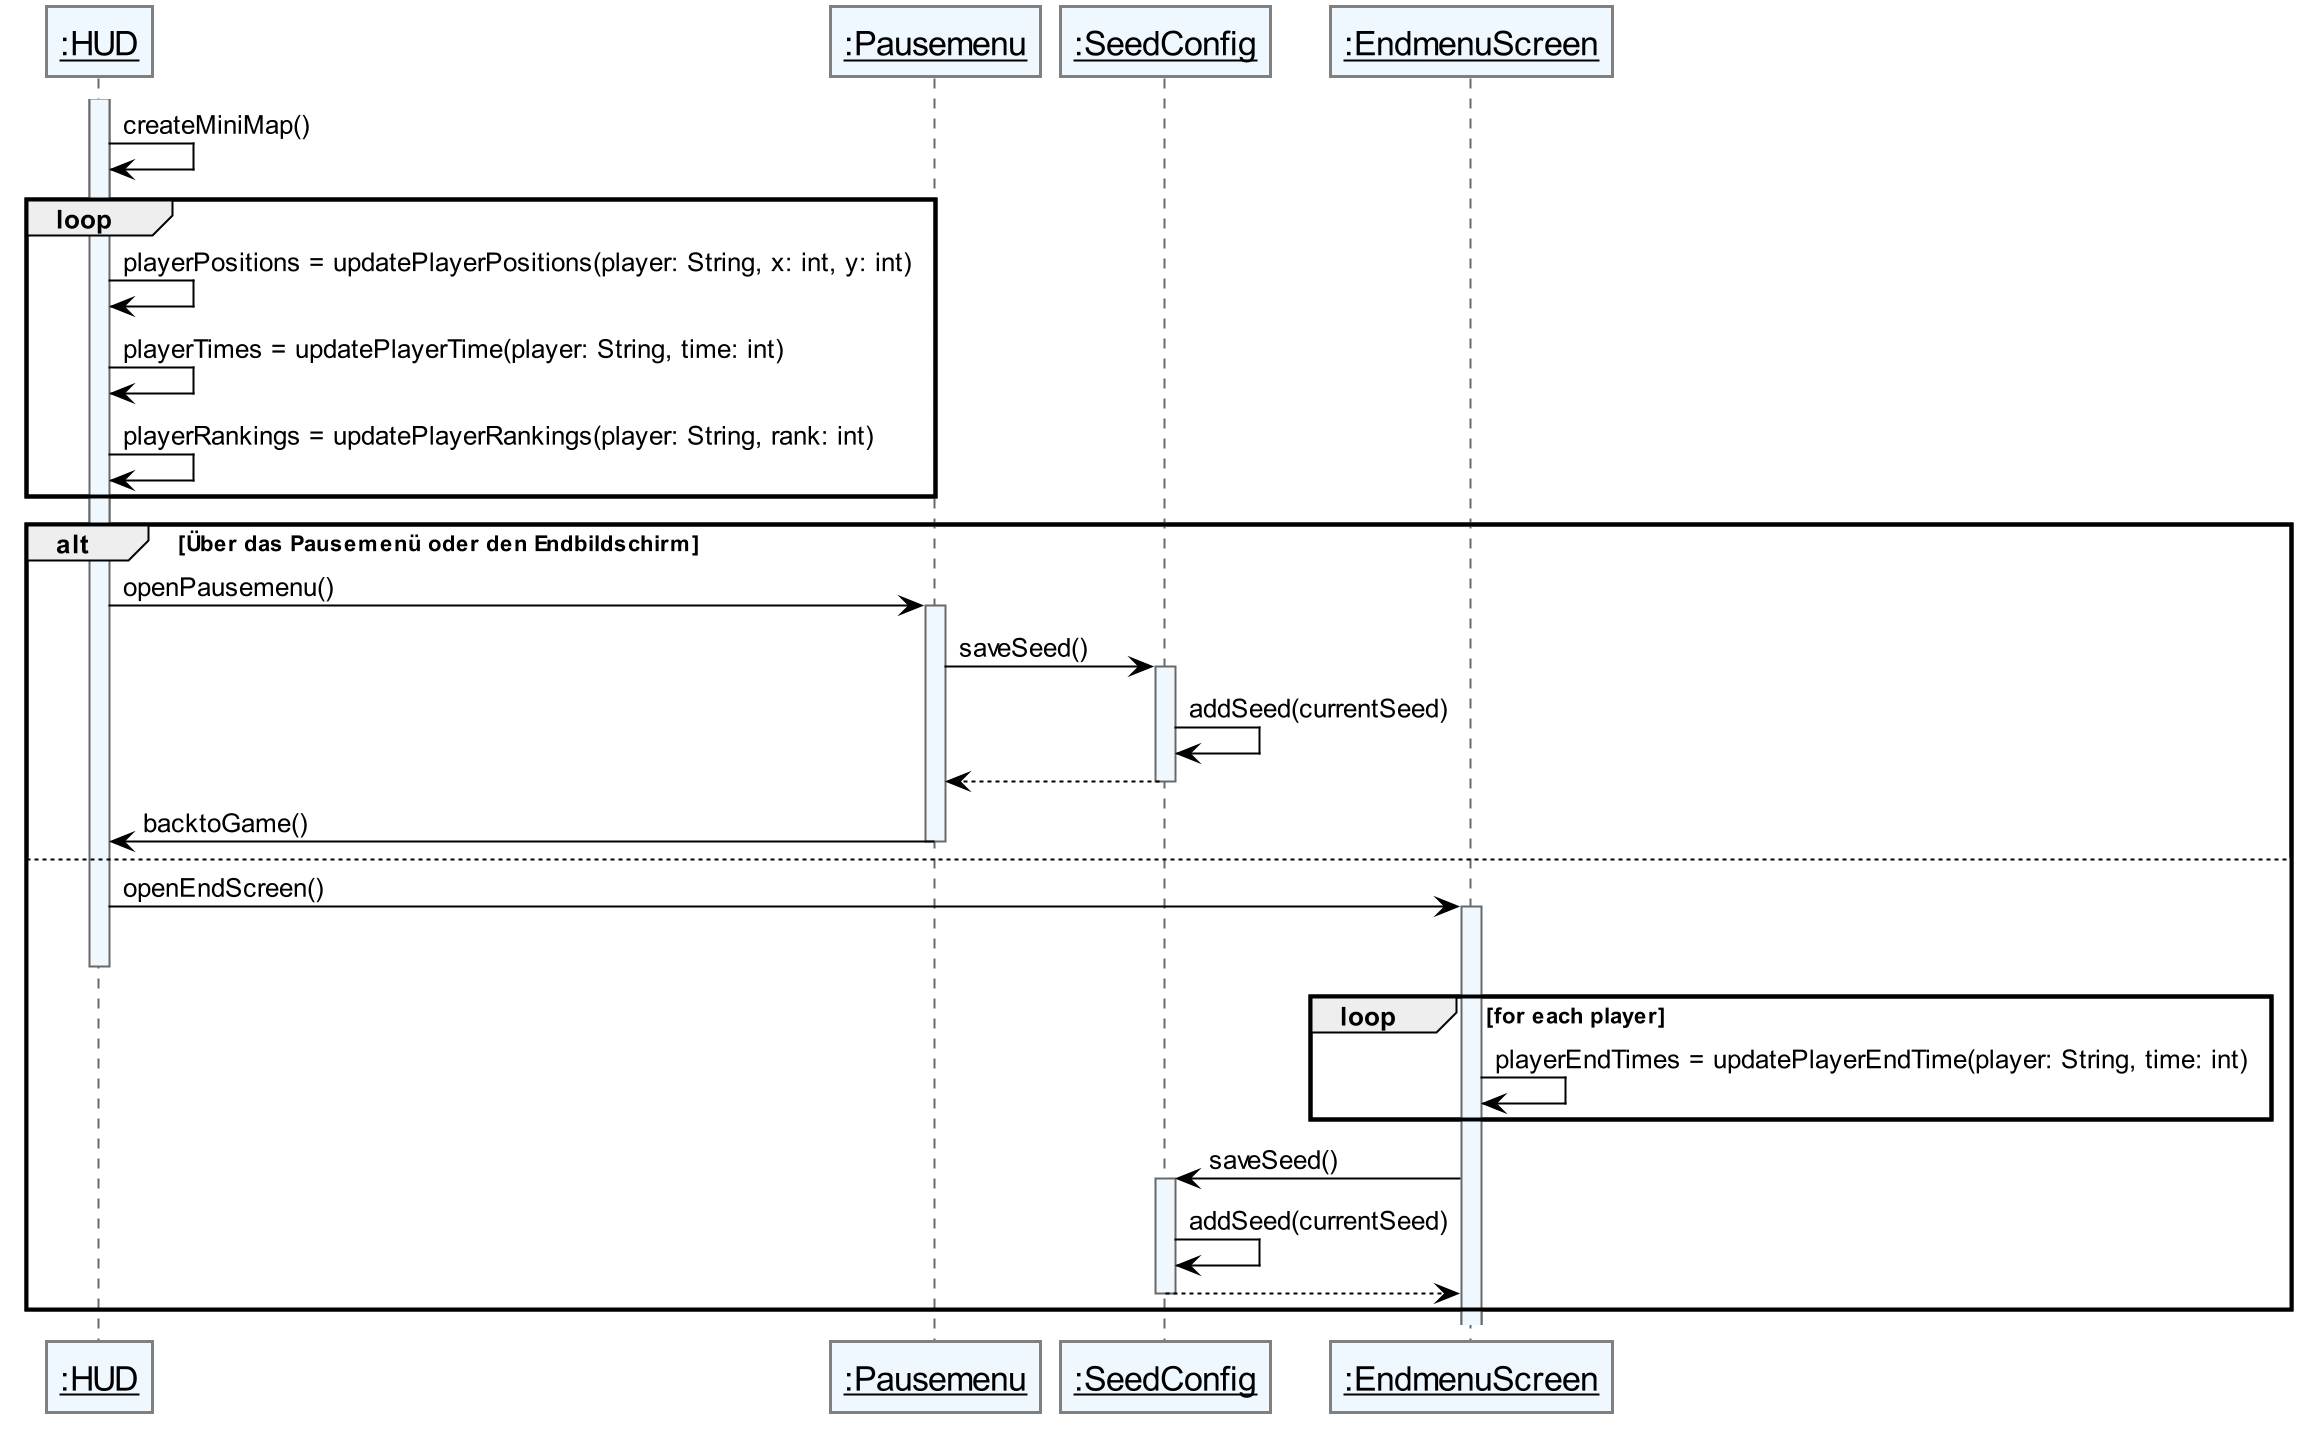
\includegraphics[width=\linewidth]{./GUI/GUI_Bilder/SaveSeed.png}
    \captionof{figure}{Den aktuell gespielten Seed speichern}
    \label{fig:SaveSeed}

\end{center}



		\pagebreak
		
	\section{Gantt - Diagramm}
		
	\begin{figure}[htbp]
		\centering
		\includegraphics[width=\linewidth]{./Bilder/PSE_Gantt.pdf}
		\caption{Gantt - Diagramm}
	\end{figure}
		
	\invisiblesection{Umfassendes Klassendiagramm}
	
	%OberMegaAllufassendesKlassendiagrammVomPumelChaosDesTodes hier einfügen
	\storeareas\myvaluesER
	\clearpage
	\KOMAoptions{paper=A0,pagesize,paper=landscape}
	\recalctypearea
	\thispagestyle{empty}
	\areaset{\dimexpr \textwidth+.6\paperwidth}{\dimexpr \textheight+.6\paperheight}
	
		\begin{figure}[htbp]
			\centering
			\includegraphics[scale=0.9,angle=0]{./Bilder/UML_Komplett.pdf}
			\caption{Klassendiagramm(komplett)}
		\end{figure}
	
	\clearpage
	\KOMAoptions{paper=A4,pagesize,paper=portrait}
	\recalctypearea
	\myvaluesER
	
	
	
\end{document}